\clearpage
\bookpart{概率极限}{Probability Limits}
\label{part:probability-limits}

\BookPartGuide{%
反复掷一枚均匀硬币，正面的比例会越来越接近二分之一；把许多独立的小误差加起来，总误差的直方图会呈现钟形。这两种现象分别回答“平均是否稳定”和“波动服从什么规律”，它们都需要先说清随机量“趋近”的含义。

第~\ref{chap:random-variable-convergence}章在同一概率空间上比较几乎必然、依概率和平均意义下的收敛，并研究期望与极限何时可以交换。第~\ref{chap:laws-of-large-numbers}章由此研究独立随机量的部分和，给出随机级数的收敛判据和大数律。

第~\ref{chap:weak-convergence-of-distributions}章换一个角度，只看分布本身怎样逼近，建立弱收敛、紧性以及特征函数等识别工具。第~\ref{chap:central-limit-theorem}章用这些工具证明中心极限定理，并估计有限样本时正态近似的误差。}

\chapter{随机变量列的收敛}
\label{chap:random-variable-convergence}

反复从$[0,1)$中均匀地随机取数，记下前$n$个数中的最大值$M_n$。取的数越多，最大值越接近$1$，这一点很少有人怀疑。可是“$M_n$趋于$1$”到底说的是什么？$M_n$不是一个数，而是随抽取结果变化的随机变量；说它“趋于”某个值，必须先说清楚在什么意义下比较它与目标的差。

至少有三种自然的读法。第一种盯住一次完整的抽取记录：记录固定以后，$M_1,M_2,\dots$是一列普通的数，问这列数是否收敛。第二种固定样本量$n$，问误差超过某个阈值的机会有多大，再看这个机会是否随$n$消失。第三种也固定$n$，但问误差的平均大小，例如平均绝对误差或均方误差是否趋于零。

对$M_n$来说三种读法给出相同的回答，但它们一般并不等价。有的随机变量列误差超标的机会越来越小，却在每一条抽取记录上都反复超标；有的随机变量列在每条记录上最终都归于零，平均误差却始终不变。前者缺的是对整条记录的控制，后者缺的是对稀有大取值的控制。

本章先在同一个概率空间上给出三种收敛方式：几乎必然收敛、依概率收敛和$L^{p}$收敛，并用几个可以手算的例子逐一检验它们之间的蕴含关系与反例。随后研究怎样判断几乎必然收敛：把“误差最终变小”改写为“超差事件只发生有限次”，由此得到Borel–Cantelli引理和子列刻画。最后研究期望能否与极限交换，依次讨论单调性、共同上界和一致可积性各自提供的保证，得到$L^{1}$收敛的判据。

\section{收敛方式}
\label{sec:rvconv-modes}

全章固定一个概率空间$(\Omega,\mathcal{F},\mathbb{P})$，在它上面讨论实随机变量$X_1,X_2,\dots$和一个候选极限$X$，它们都取有限实数值。要问的是$X_n$是否“趋于”$X$，所以把差
\[
 X_n-X
\]
当作共同的研究对象，称为第$n$项的误差。误差本身是$\Omega$上的函数，每个样本点$\omega$给出一个数$X_n(\omega)-X(\omega)$。

“误差趋于零”可以从三个角度提要求。逐样本：固定$\omega$，看数列$X_n(\omega)-X(\omega)$是否趋于零。逐事件：固定$n$和阈值$\varepsilon$，看误差超过$\varepsilon$这一事件的概率。逐平均：固定$n$，看误差绝对值的某次幂的期望。三个角度依次给出本节的三种收敛方式。

函数列的逐点、依测度与$L^{p}$收敛已经在一般测度空间上建立，可参考\BookChapterRef{chap:function-normed-spaces}{卷四第11章“赋范空间”}。本节不重复一般的定义和证明，而是在总质量为一的概率空间上解释每一种要求控制了什么、放过了什么。

\paragraph{贯穿全章的例子}
设$U_1,U_2,\dots$是相互独立的$\operatorname{Unif}(0,1)$随机变量，它们可以定义在同一个概率空间上（独立序列的构造见第~\ref{chap:probability-spaces}章），并记$U=U_1$。由它们构造下面几族随机变量，全章反复使用。第一族是累计最大值，第二族是独立示性变量，其中$p_n\in[0,1]$，$A_n=\{U_n<p_n\}$：
\[
 M_n=\max\{U_1,\dots,U_n\},\qquad \xi_n=\mathbf{1}_{A_n} .
\]
第三族是稀有大值：
\[
 Y_n=n\,\mathbf{1}_{\{U<1/n\}},\qquad Z_n=\sqrt{n}\,\mathbf{1}_{\{U<1/n\}} .
\]
第四族是移动区块$B_n$：第$k$层把$[0,1)$等分为$k$段，依次取各段的示性函数，具体写法见第~\ref{sec:rvconv-convergence-in-probability}小节。$M_n$的候选极限是常数$1$，其余几族的候选极限都是$0$。
$M_n$在三种意义下都收敛，其余几族各在某些意义下不收敛，用来检验各种收敛方式的边界。

\subsection{几乎必然收敛}
\label{sec:rvconv-almost-sure}

先把样本点$\omega$看成一次完整的观测记录。对累计最大值，$\omega$对应一串取值$U_1(\omega),U_2(\omega),\dots$，也就是无限次重复抽取的全部结果；记录一旦确定，$M_1(\omega),M_2(\omega),\dots$就是一列普通的数。图~\ref{fig:rvconv-max-paths}(a)画了五条这样的记录，每条记录上的误差$1-M_n(\omega)$都单调下降，并且迟早落到阈值$\varepsilon=0.1$以下。

\begin{BookInlineFigure}
 \centering
 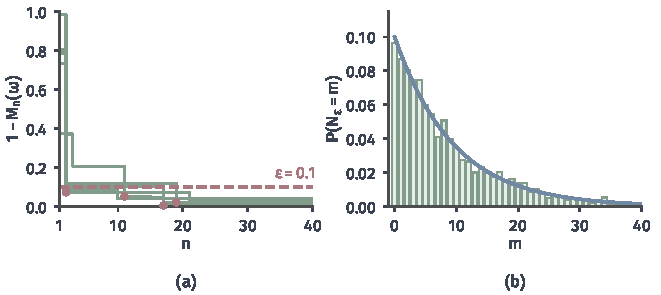
\includegraphics[width=112mm]{figures/07-probability/03-probability-limits/matplotlib/rvconv-max-paths/figure.pdf}
 \caption{累计最大值$M_n=\max\{U_1,\dots,U_n\}$的误差。(a)五条模拟记录上的$1-M_n(\omega)$（绿色台阶，种子$7$），红色虚线为阈值$\varepsilon=0.1$，红点标出误差最后一次降到阈值以下的位置。(b)最后一次超过阈值的序号$N_{\varepsilon}$：浅绿柱为$4000$条模拟记录的频率（种子$11$），蓝线为精确的质量$0.9^{m}\times0.1$。}
 \label{fig:rvconv-max-paths}
\end{BookInlineFigure}

\paragraph{例外的记录}
是不是每一条记录都如此？不是。若一条记录上所有$U_i(\omega)$都不超过$0.9$，比如每次都取到$0.5$，那么$M_n(\omega)\leq0.9$对一切$n$成立，误差永远不小于$0.1$。这样的记录是存在的，问题是它们一共有多大的概率。

$M_n(\omega)$随$n$递增且不超过$1$，所以它总收敛到$\sup_iU_i(\omega)$。它不收敛到$1$，当且仅当$\sup_iU_i(\omega)<1$，也就是存在正整数$k$，使所有$U_i(\omega)\leq1-1/k$。对固定的$k$和任意$n$，由独立性，
\[
 \mathbb{P}\bigl(U_i\leq1-\tfrac1k\text{ 对一切 }i\bigr)\leq\mathbb{P}\bigl(U_1\leq1-\tfrac1k,\dots,U_n\leq1-\tfrac1k\bigr)=\Bigl(1-\frac1k\Bigr)^{n}.
\]
右边随$n\to\infty$趋于零，左边与$n$无关，所以左边为零。再对$k=1,2,\dots$取并，可数个零概率事件的并仍是零概率事件，于是
\[
 \mathbb{P}\bigl(M_n\not\to1\bigr)=0 .
\]
例外的记录确实存在，但它们合在一起的概率为零。

\paragraph{定义}
这正是几乎必然收敛的含义：允许一个零概率的例外集合，在它之外，每条记录上的数列都收敛到目标。

\begin{definition}[几乎必然收敛]
\label{def:rvconv-almost-sure}
若
\begin{equation}
 \mathbb{P}\bigl(\{\omega:X_n(\omega)\to X(\omega)\}\bigr)=1 ,
 \label{eq:rvconv-almost-sure}
\end{equation}
称$X_n$\term{几乎必然收敛}（almost sure convergence）到$X$，记作$X_n\xrightarrow{\mathrm{a.s.}}X$。
\end{definition}

式~\eqref{eq:rvconv-almost-sure}里的集合是由可数次集合运算得到的事件，第~\ref{sec:rvconv-infinitely-often}小节会把它写出来。几乎必然收敛就是卷四所说的几乎处处收敛，只是测度换成了概率：例外集合$\{X_n\not\to X\}$是零概率事件。

\paragraph{同一个例外集}
定义里只有一个例外集合，它要容纳整列不收敛的所有记录。展开来说，存在零概率事件$N$，使得对每个$\omega\notin N$和每个$\varepsilon>0$，都有一个序号$N_{\varepsilon}(\omega)$，当$n>N_{\varepsilon}(\omega)$时
\[
 \lvert X_n(\omega)-X(\omega)\rvert\leq\varepsilon .
\]
这里$N_{\varepsilon}(\omega)$可以随记录改变，但一旦$\omega$在例外集之外，这一条记录从某项起就再也不会超差。

对累计最大值，$N_{\varepsilon}$可以取为误差最后一次超过$\varepsilon$的序号（从未超过时取$0$）。$1-M_n$随$n$递减，所以$N_{\varepsilon}\geq m$当且仅当$1-M_m>\varepsilon$，即前$m$次抽取都不超过$1-\varepsilon$。取$\varepsilon=0.1$，得到
\[
 \mathbb{P}(N_{\varepsilon}\geq m)=0.9^{m},\qquad
 \mathbb{P}(N_{\varepsilon}=m)=0.9^{m}\times0.1 .
\]
平均要等$\mathbb{E}[N_{\varepsilon}]=0.9/0.1=9$次以后误差才稳定在$0.1$以内，但个别记录要等几十次。图~\ref{fig:rvconv-max-paths}(b)的直方图和精确质量吻合：$N_{\varepsilon}$是一个处处有限的随机变量，而不是一个对所有记录都适用的常数。

\paragraph{与逐项保证的区别}
几乎必然收敛要和另一种看起来相近的说法分开。设对每个$n$，误差超标的概率都很小：
\[
 \mathbb{P}\bigl(\lvert X_n-X\rvert>\varepsilon\bigr)\leq\delta_n,\qquad \delta_n\to0 .
\]
这是对每一项分别作出的高概率保证，每一项都有自己的例外事件。这些例外事件随$n$改变，即使每一个都很小，它们也可能轮流覆盖整个$\Omega$，使得每条记录都无穷多次超标。下一小节的移动区块正是这种情形。

\paragraph{极限的唯一性}
几乎必然极限只能在零概率事件上有差别。若$X_n\xrightarrow{\mathrm{a.s.}}X$且$X_n\xrightarrow{\mathrm{a.s.}}X'$，两个收敛事件的概率都是$1$，它们的交的概率也是$1$。在交上，同一个数列的两个极限必须相等，所以
\[
 \mathbb{P}(X=X')=1 .
\]
反过来，把$X$在零概率事件上改值，几乎必然收敛不受影响。

\subsection{依概率收敛}
\label{sec:rvconv-convergence-in-probability}

几乎必然收敛要跟踪整条记录。很多时候我们只关心某个固定的样本量：抽了$n$次以后，误差大于$\varepsilon$的可能性有多大？这只涉及一个事件
\[
 \{\lvert X_n-X\rvert>\varepsilon\},
\]
称为第$n$项的超差事件。它是$\Omega$中的一个集合，大小用概率衡量。

对累计最大值，超差事件是
\[
 \{1-M_n>\varepsilon\}=\{U_1\leq1-\varepsilon,\dots,U_n\leq1-\varepsilon\},
\]
在$(U_1,\dots,U_n)$的单位立方体里是一个边长$1-\varepsilon$的小立方体。由独立性，它的概率是
\begin{equation}
 \mathbb{P}(1-M_n>\varepsilon)=(1-\varepsilon)^{n} .
 \label{eq:rvconv-max-tail}
\end{equation}
取$\varepsilon=0.1$，前三项是$0.9$、$0.81$、$0.729$，见图~\ref{fig:rvconv-error-event}；$n=10$时约为$0.3487$，$n=50$时约为$0.0052$。

\begin{BookInlineFigure}
 \centering
 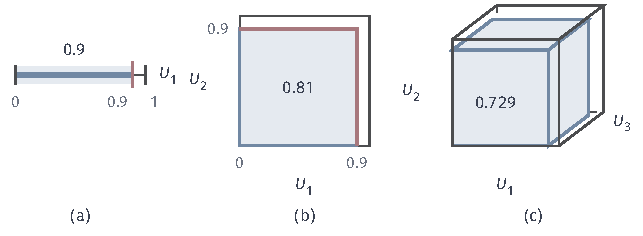
\includegraphics[width=109mm]{figures/07-probability/03-probability-limits/tikz/rvconv-error-event/figure.pdf}
 \caption{累计最大值的超差事件$\{1-M_n>0.1\}$。(a)$n=1$：线段$[0,0.9]$。(b)$n=2$：单位正方形中边长$0.9$的正方形，红线是事件的边界。(c)$n=3$：单位立方体中边长$0.9$的立方体。浅蓝区域的概率依次为$0.9$、$0.81$、$0.729$。}
 \label{fig:rvconv-error-event}
\end{BookInlineFigure}

\begin{definition}[依概率收敛]
\label{def:rvconv-in-probability}
若对每个$\varepsilon>0$，
\begin{equation}
 \lim_{n\to\infty}\mathbb{P}\bigl(\lvert X_n-X\rvert>\varepsilon\bigr)=0 ,
 \label{eq:rvconv-in-probability}
\end{equation}
称$X_n$\term{依概率收敛}（convergence in probability）到$X$，记作$X_n\xrightarrow{\mathbb{P}}X$。
\end{definition}

把“$>\varepsilon$”换成“$\geq\varepsilon$”得到同一个概念，因为两种事件互相夹住：
\[
 \{\lvert X_n-X\rvert>\varepsilon\}\subseteq\{\lvert X_n-X\rvert\geq\varepsilon\}\subseteq\{\lvert X_n-X\rvert>\varepsilon/2\} .
\]
由式~\eqref{eq:rvconv-max-tail}，$M_n\xrightarrow{\mathbb{P}}1$。依概率收敛就是卷四的依测度收敛，测度换成了概率。

\paragraph{移动区块}
依概率收敛只要求每一项的超差事件变小，并不要求它们停在同一个地方。下面的例子让超差事件在$\Omega$上来回移动。对$k=1,2,\dots$与$j=0,1,\dots,k-1$，令第$k$层第$j$段为$[j/k,(j+1)/k)$，按层从小到大、层内从左到右排成一列。第$n$项对应
\[
 n=\frac{k(k-1)}{2}+j+1,\qquad B_n=\mathbf{1}_{\{j/k\leq U<(j+1)/k\}} .
\]
前几项依次是$\mathbf{1}_{[0,1)}(U)$、$\mathbf{1}_{[0,1/2)}(U)$、$\mathbf{1}_{[1/2,1)}(U)$、$\mathbf{1}_{[0,1/3)}(U)$，等等。

对$0<\varepsilon<1$，第$n$项的超差事件就是$U$落在当前那一段，概率是段长$1/k$。$n$增大时层号$k$趋于无穷，所以
\[
 \mathbb{P}(\lvert B_n\rvert>\varepsilon)=\frac1k\to0,\qquad B_n\xrightarrow{\mathbb{P}}0 .
\]

但每一层的$k$段恰好铺满$[0,1)$，无论$U(\omega)$取什么值，每一层里都恰有一项等于$1$。所以对每一个$\omega$，数列$B_n(\omega)$中$1$出现无穷多次，$0$也出现无穷多次，它在任何一条记录上都不收敛。取$U(\omega)=0.37$，第$k$层里取值为$1$的是$j=\lfloor0.37k\rfloor$那一项，前几个序号是
\[
 n=1,\ 2,\ 5,\ 8,\ 12,\ 18,\ 24,\ 31,\ \dots
\]

\begin{BookInlineFigure}
 \centering
 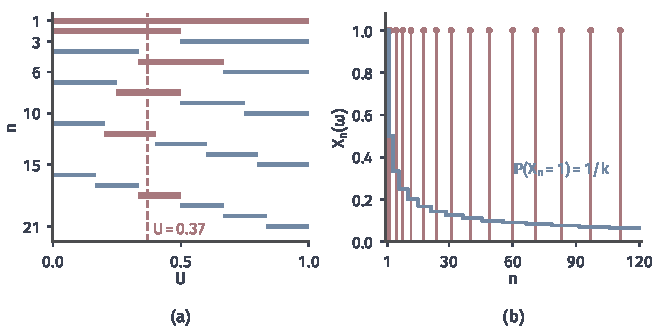
\includegraphics[width=112mm]{figures/07-probability/03-probability-limits/matplotlib/rvconv-blocks/figure.pdf}
 \caption{移动区块$B_n$。(a)前六层共$21$项：第$n$行的横条是$\{B_n=1\}$对应的$U$值区间，红色横条是被$U=0.37$穿过的那一项。(b)$U=0.37$这条记录上的$B_n(\omega)$，$n\leq120$：红色竖线标出取值为$1$的项；蓝色台阶是超差概率$\mathbb{P}(B_n=1)=1/k$。}
 \label{fig:rvconv-blocks}
\end{BookInlineFigure}

图~\ref{fig:rvconv-blocks}把两种读法放在一起。(a)中逐行看，每一行的横条越来越短，这是依概率收敛控制的量；沿红色虚线竖着看，就是一条记录，每一层都要碰到一个横条。(b)中蓝色台阶趋于零，红线却永不消失。大误差总会发生，只是发生在哪些记录上随$n$改变。

\paragraph{与几乎必然收敛对照}
两种收敛的差别在于控制的对象。依概率收敛逐次控制超差事件的大小，每个$n$单独检查；几乎必然收敛控制每条记录最终的行为，要求同一个$\omega$在某项之后再也不落入超差事件。前者是“在每一时刻，出问题的记录很少”，后者是“几乎每条记录，迟早不再出问题”。第~\ref{sec:rvconv-comparison}节证明后者推出前者，移动区块说明反过来不成立。

\paragraph{极限的唯一性与和的收敛}
依概率极限同样只在零概率事件上有差别。若$X_n\xrightarrow{\mathbb{P}}X$且$X_n\xrightarrow{\mathbb{P}}X'$，由三角不等式，$\lvert X-X'\rvert>2\varepsilon$时$\lvert X_n-X\rvert$与$\lvert X_n-X'\rvert$至少有一个大于$\varepsilon$，所以
\[
 \mathbb{P}\bigl(\lvert X-X'\rvert>2\varepsilon\bigr)\leq\mathbb{P}\bigl(\lvert X_n-X\rvert>\varepsilon\bigr)+\mathbb{P}\bigl(\lvert X_n-X'\rvert>\varepsilon\bigr).
\]
右边趋于零，左边与$n$无关，故为零。令$\varepsilon=1/k$并对$k$取可数并，得$\mathbb{P}(X\neq X')=0$。

同样的论证给出和的收敛：若$X_n\xrightarrow{\mathbb{P}}X$，$Y_n\xrightarrow{\mathbb{P}}Y$，则
\[
 \mathbb{P}\bigl(\lvert(X_n+Y_n)-(X+Y)\rvert>2\varepsilon\bigr)\leq\mathbb{P}\bigl(\lvert X_n-X\rvert>\varepsilon\bigr)+\mathbb{P}\bigl(\lvert Y_n-Y\rvert>\varepsilon\bigr)\to0 ,
\]
即$X_n+Y_n\xrightarrow{\mathbb{P}}X+Y$。两个超差事件各自很小，它们的并也很小，这种“并集上界”是处理依概率收敛的基本手段。

\subsection{\texorpdfstring{$L^{p}$}{Lp}收敛}
\label{sec:rvconv-lp}

超差概率只数大误差出现的机会，不管大误差有多大。另一种自然的要求是误差的平均大小趋于零。对$1\leq p<\infty$，误差绝对值的$p$次幂取期望，得到一个数$\mathbb{E}\bigl[\lvert X_n-X\rvert^{p}\bigr]$，大误差在其中按$p$次幂加权。

\begin{definition}[$L^{p}$收敛]
\label{def:rvconv-lp}
设$1\leq p<\infty$，$\mathbb{E}[\lvert X\rvert^{p}]<\infty$，且对每个$n$有$\mathbb{E}[\lvert X_n\rvert^{p}]<\infty$。若
\begin{equation}
 \lim_{n\to\infty}\mathbb{E}\bigl[\lvert X_n-X\rvert^{p}\bigr]=0 ,
 \label{eq:rvconv-lp}
\end{equation}
称$X_n$\term{$L^p$收敛}（convergence in $L^p$）到$X$，记作$X_n\xrightarrow{L^{p}}X$。
\end{definition}

矩有限的假设保证误差的$p$阶矩有意义。由$t\mapsto t^{p}$的凸性，对实数$a,b$有
\[
 \lvert a-b\rvert^{p}\leq2^{p-1}\bigl(\lvert a\rvert^{p}+\lvert b\rvert^{p}\bigr),
\]
所以$X_n$与$X$的$p$阶矩有限时，误差的$p$阶矩也有限。

把$p$阶矩开$p$次方，记
\[
 \lVert X\rVert_{p}=\bigl(\mathbb{E}[\lvert X\rvert^{p}]\bigr)^{1/p} ,
\]
它是卷四$L^{p}$范数在概率空间上的写法，$L^{p}$收敛就是$\lVert X_n-X\rVert_{p}\to0$。若同一列还$L^{p}$收敛到$X'$，由Minkowski不等式，
\[
 \lVert X-X'\rVert_{p}\leq\lVert X_n-X\rVert_{p}+\lVert X_n-X'\rVert_{p}\to0 ,
\]
左边与$n$无关，故为零，$X=X'$几乎必然。

\paragraph{平均绝对误差与均方误差}
$p=1$时，$\mathbb{E}[\lvert X_n-X\rvert]$是\emph{平均绝对误差}；$p=2$时，$\mathbb{E}[(X_n-X)^{2}]$是\emph{均方误差}，$L^{2}$收敛也称\term{均方收敛}（mean-square convergence）。目标是常数$c$时，均方误差可以拆成方差与偏差平方之和。在$X_n-c=(X_n-\mathbb{E}[X_n])+(\mathbb{E}[X_n]-c)$两边平方取期望，交叉项的期望为零，得到
\begin{equation}
 \mathbb{E}\bigl[(X_n-c)^{2}\bigr]=\operatorname{Var}(X_n)+\bigl(\mathbb{E}[X_n]-c\bigr)^{2} .
 \label{eq:rvconv-mse}
\end{equation}
所以$X_n\xrightarrow{L^{2}}c$当且仅当$\mathbb{E}[X_n]\to c$且$\operatorname{Var}(X_n)\to0$：均值要对准目标，波动要消失。

\paragraph{累计最大值的平均误差}
非负变量的矩可以由尾积分公式（第~\ref{chap:tail-probabilities}章）从生存函数算出：
\[
 \mathbb{E}[V^{p}]=\int_0^{\infty}p\,t^{p-1}\,\mathbb{P}(V>t)\,\mathrm{d}t .
\]
取$V=1-M_n$，它在$[0,1]$内取值，生存函数由式~\eqref{eq:rvconv-max-tail}给出。$p=1$时，
\[
 \mathbb{E}[1-M_n]=\int_0^{1}(1-t)^{n}\,\mathrm{d}t=\frac{1}{n+1} .
\]

$p=2$时，把$t=1-(1-t)$代入并分成两个积分，得到
\[
 \mathbb{E}\bigl[(1-M_n)^{2}\bigr]=2\int_0^{1}t(1-t)^{n}\,\mathrm{d}t=2\Bigl(\frac{1}{n+1}-\frac{1}{n+2}\Bigr)=\frac{2}{(n+1)(n+2)} .
\]
两者都趋于零，所以$M_n\xrightarrow{L^{1}}1$，$M_n\xrightarrow{L^{2}}1$。取$n=10$，平均绝对误差是$1/11\approx0.0909$，均方误差是$2/132\approx0.0152$。

用式~\eqref{eq:rvconv-mse}核对。偏差是$\mathbb{E}[M_{10}]-1=-1/11$，方差是均方误差减去偏差平方：
\[
 \operatorname{Var}(M_{10})=\frac{2}{132}-\frac{1}{121}\approx0.01515-0.00826=0.00689 .
\]
两部分大小相当：$M_n$总是低估$1$，平均低估$1/(n+1)$，同时围绕自己的均值波动。

\paragraph{稀有大值}
$L^{p}$收敛对大误差特别敏感。看$Z_n=\sqrt{n}\,\mathbf{1}_{\{U<1/n\}}$：它以概率$1/n$取$\sqrt n$，其余时候取$0$，所以
\begin{equation}
 \mathbb{E}\bigl[\lvert Z_n\rvert^{p}\bigr]=n^{p/2}\cdot\frac1n=n^{p/2-1} .
 \label{eq:rvconv-spike-moments}
\end{equation}
$p=1$时这是$n^{-1/2}\to0$，$p=2$时恒为$1$，$p=3$时是$n^{1/2}\to\infty$。同一列变量$L^{1}$收敛到$0$，却不$L^{2}$收敛。

把高度换成$n$，$Y_n=n\,\mathbf{1}_{\{U<1/n\}}$的平均绝对误差恒为$\mathbb{E}[Y_n]=1$，连$L^{1}$收敛也不成立。另一方面，$Y_n$与$Z_n$都在$U\geq1/n$时为零；对任何$U(\omega)>0$，$n>1/U(\omega)$以后两者都等于$0$，而$\mathbb{P}(U=0)=0$，所以它们都几乎必然收敛到$0$。超差概率是$1/n$，它们也依概率收敛到$0$。误差发生得越来越少，但每次发生时越来越大，平均误差能否消失取决于“少”与“大”谁占上风，而$p$越大，大误差的分量越重。

移动区块则相反：误差只取$0$和$1$，没有大值，$\mathbb{E}[\lvert B_n\rvert^{p}]=1/k\to0$，所以它在每个$L^{p}$中收敛到$0$，尽管在任何一条记录上都不收敛。

\paragraph{随机向量}
以上三种收敛对随机向量$\bm{X}_n,\bm{X}\in\mathbb{R}^{d}$同样适用，只需把$\lvert X_n-X\rvert$换成欧氏范数$\lVert\bm{X}_n-\bm{X}\rVert_2$。由于对每个分量$i$都有
\[
 \lvert x_i\rvert\leq\lVert\bm{x}\rVert_2\leq\lvert x_1\rvert+\dots+\lvert x_d\rvert ,
\]
向量的每一种收敛都等价于各个分量的同种收敛。维数固定时，只需研究实随机变量。


\section{收敛方式的比较}
\label{sec:rvconv-comparison}

三种收敛控制的对象不同：几乎必然收敛管每条记录的最终行为，依概率收敛管每一项超差事件的大小，$L^{p}$收敛管误差的平均大小。上一节的例子已经显示它们并不等价。哪些要求能推出另一些？推不出时，缺的是哪一种控制？

在一般测度空间上，几乎处处收敛推出依测度收敛需要总测度有限，$L^{r}$收敛推出较低阶的$L^{p}$收敛也需要总测度有限。概率空间的总质量为一，这两个条件自动满足，于是得到下面三条蕴含关系。

\begin{theorem}[收敛方式的蕴含关系]
\label{thm:rvconv-implications}
设$X_n,X$是同一概率空间上的实随机变量，$1\leq p<r<\infty$。
\begin{enumerate}
 \item 若$X_n\xrightarrow{\mathrm{a.s.}}X$，则$X_n\xrightarrow{\mathbb{P}}X$。
 \item 若$X_n\xrightarrow{L^{p}}X$，则$X_n\xrightarrow{\mathbb{P}}X$；更具体地，对每个$\varepsilon>0$，
 \begin{equation}
  \mathbb{P}\bigl(\lvert X_n-X\rvert>\varepsilon\bigr)\leq\frac{\mathbb{E}\bigl[\lvert X_n-X\rvert^{p}\bigr]}{\varepsilon^{p}} .
  \label{eq:rvconv-markov-lp}
 \end{equation}
 \item 若$X_n\xrightarrow{L^{r}}X$，则$X_n\xrightarrow{L^{p}}X$；更具体地，
 \begin{equation}
  \lVert X_n-X\rVert_{p}\leq\lVert X_n-X\rVert_{r} .
  \label{eq:rvconv-lp-monotone}
 \end{equation}
\end{enumerate}
\end{theorem}

\begin{proof}
第1条。固定$\varepsilon>0$，令
\[
 G_N=\bigcup_{n\geq N}\bigl\{\lvert X_n-X\rvert>\varepsilon\bigr\},
\]
即从第$N$项起至少超差一次的记录。$G_N$随$N$递减。若$\omega$属于每一个$G_N$，则$\omega$上超差发生无穷多次，$X_n(\omega)\not\to X(\omega)$；所以$\bigcap_NG_N\subseteq\{X_n\not\to X\}$，它的概率为零。

概率测度对递减事件列连续（第~\ref{chap:probability-spaces}章），这里用到总质量有限：
\[
 \mathbb{P}(G_N)\to\mathbb{P}\Bigl(\bigcap_NG_N\Bigr)=0 .
\]
而第$N$项的超差事件含于$G_N$，它的概率不超过$\mathbb{P}(G_N)$，也趋于零。

第2条。超差事件含于$p$次幂的超差事件：
\[
 \{\lvert X_n-X\rvert>\varepsilon\}\subseteq\{\lvert X_n-X\rvert^{p}\geq\varepsilon^{p}\} .
\]
对非负随机变量$\lvert X_n-X\rvert^{p}$和阈值$\varepsilon^{p}$用Markov不等式（第~\ref{chap:tail-probabilities}章），即得式~\eqref{eq:rvconv-markov-lp}。右边趋于零，左边也趋于零。

第3条。第~\ref{chap:random-variable-moments}章由Jensen不等式证明了绝对矩开相应次方后随阶数单调增加：对任意随机变量$V$，
\[
 \bigl(\mathbb{E}[\lvert V\rvert^{p}]\bigr)^{1/p}\leq\bigl(\mathbb{E}[\lvert V\rvert^{r}]\bigr)^{1/r} .
\]
取$V=X_n-X$即得式~\eqref{eq:rvconv-lp-monotone}。
\end{proof}

第1条证明中的$G_N$把整个尾段的超差合在一起。几乎必然收敛控制的正是这个尾段的并，依概率收敛只控制其中一项，前者自然更强；第~\ref{sec:rvconv-infinitely-often}小节会把这一观察写成等价条件。第3条在一般测度空间上要多出一个因子，即总测度的$1/p-1/r$次幂，概率空间中这个因子是$1$。

\paragraph{用累计最大值核对}
取$n=10$，$\varepsilon=0.1$。精确的超差概率是$0.9^{10}\approx0.349$。由式~\eqref{eq:rvconv-markov-lp}，用平均绝对误差$1/11$与均方误差$2/132$分别得到上界
\[
 \frac{1/11}{0.1}\approx0.909,\qquad \frac{2/132}{0.01}\approx1.52 .
\]
两个界都成立，后者大于$1$而没有信息。式~\eqref{eq:rvconv-lp-monotone}也可以直接核对：
\[
 \lVert1-M_{10}\rVert_{1}\approx0.0909\leq\lVert1-M_{10}\rVert_{2}=\sqrt{2/132}\approx0.123 .
\]

\paragraph{逆命题的反例}
三条蕴含关系都不能反过来。表~\ref{tab:rvconv-examples}汇总了贯穿例子的收敛情况，其中独立示性变量$\xi_n$取$p_n=1/n$，它不几乎必然收敛这一点要到第~\ref{sec:rvconv-borel-cantelli}小节才能证明。

\begin{BookInlineTable}
 \centering
 \begin{tabular}{@{}lcccc@{}}
  \toprule
  随机变量列 & 几乎必然 & 依概率 & $L^{1}$ & $L^{2}$ \\
  \midrule
  $M_n\to1$ & 是 & 是 & 是 & 是 \\
  移动区块$B_n\to0$ & 否 & 是 & 是 & 是 \\
  $\xi_n\to0$，$p_n=1/n$ & 否 & 是 & 是 & 是 \\
  $Z_n=\sqrt n\,\mathbf{1}_{\{U<1/n\}}\to0$ & 是 & 是 & 是 & 否 \\
  $Y_n=n\,\mathbf{1}_{\{U<1/n\}}\to0$ & 是 & 是 & 否 & 否 \\
  \bottomrule
 \end{tabular}
 \caption{贯穿例子在四种意义下是否收敛。}
 \label{tab:rvconv-examples}
\end{BookInlineTable}

表中的“否”来自两种不同的缺陷。第一种是缺少尾部控制：$Y_n$和$Z_n$的超差概率$1/n$趋于零，每条记录最终也归于零，但偶尔出现的误差越来越大，大到足以维持平均。依概率收敛与几乎必然收敛都只看误差是否超过$\varepsilon$，对超出多少一无所知，所以推不出$L^{p}$收敛。

第二种是缺少整列的逐样本控制：$B_n$和$\xi_n$的误差只取$0$或$1$，平均误差和超差概率一起趋于零，但超差事件在$\Omega$上不断移动或独立地重新出现，每条记录（或几乎每条记录）上都无穷多次超差。$L^{p}$收敛与依概率收敛都是逐项的要求，管不到同一条记录在不同时刻的表现，所以推不出几乎必然收敛。

\begin{BookInlineFigure}
 \centering
 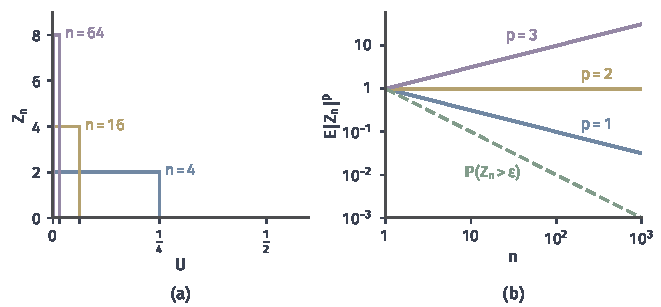
\includegraphics[width=112mm]{figures/07-probability/03-probability-limits/matplotlib/rvconv-power-spikes/figure.pdf}
 \caption{稀有大值$Z_n=\sqrt n\,\mathbf{1}_{\{U<1/n\}}$。(a)$Z_n$作为$U$的函数，$n=4,16,64$：高为$\sqrt n$、宽为$1/n$的矩形。(b)双对数坐标下的精确矩$\mathbb{E}[\lvert Z_n\rvert^{p}]=n^{p/2-1}$，$p=1,2,3$（蓝、黄、紫），绿色虚线是超差概率$1/n$（$0<\varepsilon<1$）。}
 \label{fig:rvconv-power-spikes}
\end{BookInlineFigure}

图~\ref{fig:rvconv-power-spikes}把第一种缺陷画出来。(a)中矩形越来越窄、越来越高；$p$阶矩是$\lvert Z_n\rvert^{p}$下方的面积，宽度按$1/n$缩小，高度的$p$次幂按$n^{p/2}$增长。(b)中各条直线的斜率$p/2-1$表明两者谁占上风：$p<2$时宽度胜出，$p=2$时恰好持平，$p>2$时高度胜出。超差概率的斜率是$-1$，它对高度完全不敏感。

\paragraph{较高阶与较低阶}
$Z_n$还说明第3条不能反过来：$L^{1}$收敛推不出$L^{2}$收敛。较低阶的平均把大误差压得较轻，较高阶的平均把它放得较重，所以控制高阶误差的要求更强。

\paragraph{两种收敛同时成立时}
若同一列变量既几乎必然收敛到$X$，又$L^{p}$收敛到$X'$，则由定理~\ref{thm:rvconv-implications}，两者都推出依概率收敛，再由依概率极限的唯一性，$X=X'$几乎必然。不同的收敛方式可能有的成立、有的不成立，但只要成立，极限就相同。

缺陷既然分成两种，就可以分别去补。超差事件如何才能只在每条记录上出现有限次？这是下一节的问题，答案依赖超差概率加起来是否有限，以及各事件是否独立。什么样的尾部条件能阻止稀有大值维持平均？这是第~\ref{sec:rvconv-expectation-limits}节的问题。


\section{几乎必然收敛的判别}
\label{sec:rvconv-as-criteria}

怎样判断一列随机变量是否几乎必然收敛？定义要求几乎每条记录上的数列收敛，直接检查每条记录通常做不到。本节把问题翻译成事件的语言：误差最终小于$\varepsilon$，就是超差事件从某项起不再发生，也就是它只发生有限次。于是问题变成：一列事件在几乎每条记录上是否只发生有限次？

\subsection{无穷多次发生的事件}
\label{sec:rvconv-infinitely-often}

给定事件列$A_1,A_2,\dots$。一条记录$\omega$可能落在其中无穷多个事件里，也可能只落在有限个里。图~\ref{fig:rvconv-limsup-grid}画了四条记录：$\omega_1$落在所有偶数号事件里，$\omega_3$落在平方数号事件里，都是无穷多次；$\omega_2$只落在四个事件里；$\omega_4$从不落入。

\begin{BookInlineFigure}
 \centering
 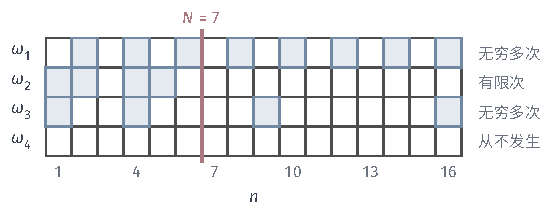
\includegraphics[width=94mm]{figures/07-probability/03-probability-limits/tikz/rvconv-limsup-grid/figure.pdf}
 \caption{事件的无穷次发生。每行是一条记录，第$n$列的浅蓝格表示该记录属于$A_n$。红线右侧是从$N=7$起的尾段：$\omega_1$与$\omega_3$在尾段中仍然出现，属于$\bigcup_{n\geq7}A_n$；$\omega_2$与$\omega_4$不属于。无论$N$取多大，$\omega_1$与$\omega_3$总留在尾段的并里。}
 \label{fig:rvconv-limsup-grid}
\end{BookInlineFigure}

“无穷多次”可以用可数次集合运算写出来。$\omega$落在无穷多个$A_n$中，等价于无论从哪一项$N$开始往后看，它都至少还落在一个$A_n$（$n\geq N$）中，即对每个$N$都有$\omega\in\bigcup_{n\geq N}A_n$。

\begin{definition}[事件的上极限与下极限]
\label{def:rvconv-limsup}
对事件列$(A_n)$，令
\begin{equation}
 \limsup_{n\to\infty}A_n=\bigcap_{N=1}^{\infty}\bigcup_{n\geq N}A_n,\qquad
 \liminf_{n\to\infty}A_n=\bigcup_{N=1}^{\infty}\bigcap_{n\geq N}A_n .
 \label{eq:rvconv-limsup}
\end{equation}
前者是$A_n$\term{无穷多次发生}（occurring infinitely often）的事件，也记作$\{A_n\ \text{i.o.}\}$；后者是从某项起$A_n$每次都发生的事件。
\end{definition}

两者都由可数次并与交得到，所以都是事件。取补集并交换并与交，得到
\[
 \Bigl(\limsup_{n\to\infty}A_n\Bigr)^{\mathrm{c}}=\bigcup_{N=1}^{\infty}\bigcap_{n\geq N}A_n^{\mathrm{c}}=\liminf_{n\to\infty}A_n^{\mathrm{c}} .
\]
右边说的是“存在$N$，从第$N$项起$A_n$不再发生”，也就是$A_n$只发生有限次。“无穷多次发生”与“最终不再发生”恰好互补。

尾段的并$\bigcup_{n\geq N}A_n$随$N$递减，由概率的连续性，
\begin{equation}
 \mathbb{P}\Bigl(\limsup_{n\to\infty}A_n\Bigr)=\lim_{N\to\infty}\mathbb{P}\Bigl(\bigcup_{n\geq N}A_n\Bigr) .
 \label{eq:rvconv-limsup-continuity}
\end{equation}
无穷多次发生的概率，就是“从第$N$项起至少再发生一次”的概率在$N\to\infty$时的极限。

\paragraph{应用于超差事件}
现在把$A_n$取为超差事件。对$\varepsilon>0$，记
\[
 A_n(\varepsilon)=\bigl\{\lvert X_n-X\rvert>\varepsilon\bigr\}.
\]
$\omega$上的数列$X_n(\omega)$收敛到$X(\omega)$，就是对每个$\varepsilon>0$，$\omega$只落在有限个$A_n(\varepsilon)$中。阈值有不可数多个，但$\varepsilon$越小超差事件越大，所以只需检查一列趋于零的阈值，例如$\varepsilon=1/k$。

\begin{theorem}[几乎必然收敛的事件判据]
\label{thm:rvconv-as-io}
以下三条等价：
\begin{enumerate}
 \item $X_n\xrightarrow{\mathrm{a.s.}}X$；
 \item 对每个$\varepsilon>0$，$\mathbb{P}\bigl(\limsup_nA_n(\varepsilon)\bigr)=0$；
 \item 对每个$\varepsilon>0$，
 \begin{equation}
  \lim_{N\to\infty}\mathbb{P}\Bigl(\sup_{n\geq N}\lvert X_n-X\rvert>\varepsilon\Bigr)=0 .
  \label{eq:rvconv-as-sup}
 \end{equation}
\end{enumerate}
并且在第2条中只需对$\varepsilon=1/k$（$k=1,2,\dots$）检查。
\end{theorem}

\begin{proof}
先写出不收敛的记录。$X_n(\omega)\not\to X(\omega)$当且仅当存在某个$k$，使$\lvert X_n(\omega)-X(\omega)\rvert>1/k$对无穷多个$n$成立。所以
\[
 \{X_n\not\to X\}=\bigcup_{k=1}^{\infty}\limsup_{n\to\infty}A_n(1/k) .
\]
右边是可数个事件的并，因此收敛集合是事件，这也补上了定义~\ref{def:rvconv-almost-sure}中可测性的说明。

1推2。对任意$\varepsilon>0$，取$k$使$1/k<\varepsilon$，则$A_n(\varepsilon)\subseteq A_n(1/k)$，于是$\limsup_nA_n(\varepsilon)$含于$\{X_n\not\to X\}$，概率为零。

2推1。只用$\varepsilon=1/k$：由上面的等式与可数次可加性，
\[
 \mathbb{P}(X_n\not\to X)\leq\sum_{k=1}^{\infty}\mathbb{P}\Bigl(\limsup_{n\to\infty}A_n(1/k)\Bigr)=0 .
\]

2与3等价。$\sup_{n\geq N}\lvert X_n-X\rvert>\varepsilon$当且仅当某个$n\geq N$使$\lvert X_n-X\rvert>\varepsilon$，所以
\[
 \Bigl\{\sup_{n\geq N}\lvert X_n-X\rvert>\varepsilon\Bigr\}=\bigcup_{n\geq N}A_n(\varepsilon) .
\]
由式~\eqref{eq:rvconv-limsup-continuity}，这个概率的极限就是$\mathbb{P}(\limsup_nA_n(\varepsilon))$。
\end{proof}

如果直接对所有$\varepsilon>0$取并，会得到不可数个事件的并，概率论不允许对它用可加性。单调性让我们只取可数个阈值，这是“阈值只需取一列趋于零的正有理数”的原因。

\paragraph{对照依概率收敛}
式~\eqref{eq:rvconv-as-sup}与依概率收敛的式~\eqref{eq:rvconv-in-probability}只差一个上确界：依概率收敛要求第$N$项的误差超标的概率趋于零，几乎必然收敛要求从第$N$项起的最大误差超标的概率趋于零。后者控制整个尾段，这再次说明它更强。

当误差的绝对值随$n$单调不增时，尾段的最大误差就是第$N$项的误差，两种收敛等价。累计最大值正是如此：$1-M_n$递减，超差事件随$n$缩小，尾段的并就是$A_N(\varepsilon)$。由式~\eqref{eq:rvconv-max-tail}，
\[
 \mathbb{P}\Bigl(\sup_{n\geq N}(1-M_n)>\varepsilon\Bigr)=(1-\varepsilon)^{N}\to0 ,
\]
这与第~\ref{sec:rvconv-almost-sure}小节的直接论证一致。移动区块则相反：每一层都铺满$[0,1)$，对$0<\varepsilon<1$和每个$N$，$\bigcup_{n\geq N}A_n(\varepsilon)=\Omega$，尾段并的概率恒为$1$。

\subsection{Borel–Cantelli引理}
\label{sec:rvconv-borel-cantelli}

上一小节把几乎必然收敛归结为$\mathbb{P}(\limsup_nA_n)=0$。尾段的并通常没有简单公式，但每个$A_n$的概率往往容易算。能否只用这些单项概率作出判断？答案取决于$\sum_n\mathbb{P}(A_n)$是否有限：有限时，用并集上界即可；无限时，还需要独立性。

\paragraph{概率可和的情形}
若各事件的概率之和有限，尾段的概率之和趋于零，尾段的并也就越来越不可能发生。

\begin{lemma}[Borel–Cantelli引理]
\label{lem:rvconv-borel-cantelli}
若事件列$(A_n)$满足$\sum_{n=1}^{\infty}\mathbb{P}(A_n)<\infty$，则
\begin{equation}
 \mathbb{P}\Bigl(\limsup_{n\to\infty}A_n\Bigr)=0 .
 \label{eq:rvconv-bc1}
\end{equation}
\end{lemma}

\begin{proof}
对每个$N$，$\limsup_nA_n\subseteq\bigcup_{n\geq N}A_n$。由可数次可加性给出的并集上界，
\[
 \mathbb{P}\Bigl(\limsup_{n\to\infty}A_n\Bigr)\leq\mathbb{P}\Bigl(\bigcup_{n\geq N}A_n\Bigr)\leq\sum_{n\geq N}\mathbb{P}(A_n) .
\]
右边是收敛级数的尾和，$N\to\infty$时趋于零，左边与$N$无关，所以为零。
\end{proof}

这个结论称为\term{Borel–Cantelli引理}（Borel–Cantelli lemma）。证明只用了并集上界，没有用到事件之间的任何关系，所以它不要求独立。级数收敛的直观含义是事件发生的平均次数有限：第~\ref{sec:rvconv-monotone}小节会证明发生次数$\sum_n\mathbf{1}_{A_n}$的期望等于$\sum_n\mathbb{P}(A_n)$，平均次数有限的计数几乎必然有限。

\paragraph{独立示性变量：概率可和}
回到独立示性变量$\xi_n=\mathbf{1}_{\{U_n<p_n\}}$，取$p_n=1/n^{2}$。级数
\[
 \sum_{n=1}^{\infty}\frac{1}{n^{2}}=\frac{\pi^{2}}{6}\approx1.645
\]
收敛，由引理~\ref{lem:rvconv-borel-cantelli}，几乎每条记录上只有有限个$\xi_n=1$。对这样的记录，从某项起$\xi_n=0$，所以$\xi_n\xrightarrow{\mathrm{a.s.}}0$。

这里的事件恰好独立，尾段并的概率也能精确算出。由独立性和补事件，对$N\geq2$，
\[
 \mathbb{P}\Bigl(\bigcup_{n=N}^{M}A_n\Bigr)=1-\prod_{n=N}^{M}\Bigl(1-\frac{1}{n^{2}}\Bigr)=1-\prod_{n=N}^{M}\frac{(n-1)(n+1)}{n\cdot n} .
\]

乘积是裂项的：分子中的$n-1$与前一项分母的$n$相消，$n+1$与后一项分母的$n$相消，只剩下首尾两个因子，
\[
 \prod_{n=N}^{M}\frac{(n-1)(n+1)}{n\cdot n}=\frac{N-1}{N}\cdot\frac{M+1}{M} .
\]
令$M\to\infty$，得到$\mathbb{P}\bigl(\bigcup_{n\geq N}A_n\bigr)=1/N$。$N=10$时它等于$0.1$，并集上界$\sum_{n\geq10}n^{-2}\approx0.105$，两者相当接近，见图~\ref{fig:rvconv-bc-unions}(a)。

\paragraph{概率不可和的情形}
级数发散时，并集上界失效。此时事件是否无穷多次发生取决于事件之间的关系。若各事件独立，发散的级数迫使它们无穷多次发生。

\begin{lemma}[独立事件的Borel–Cantelli引理]
\label{lem:rvconv-borel-cantelli-2}
若事件$A_1,A_2,\dots$相互独立，且$\sum_{n=1}^{\infty}\mathbb{P}(A_n)=\infty$，则
\begin{equation}
 \mathbb{P}\Bigl(\limsup_{n\to\infty}A_n\Bigr)=1 .
 \label{eq:rvconv-bc2}
\end{equation}
\end{lemma}

\begin{proof}
只需证明补事件的概率为零。由上一小节，补事件是
\[
 \Bigl(\limsup_{n\to\infty}A_n\Bigr)^{\mathrm{c}}=\bigcup_{N=1}^{\infty}\bigcap_{n\geq N}A_n^{\mathrm{c}} ,
\]
它是可数个事件的并，所以只需证明对每个$N$，
\[
 \mathbb{P}\Bigl(\bigcap_{n\geq N}A_n^{\mathrm{c}}\Bigr)=0 .
\]

相互独立事件的补事件仍相互独立。对$M\geq N$，记$p_n=\mathbb{P}(A_n)$，再用$1-x\leq\mathrm{e}^{-x}$（$x\in\mathbb{R}$），得到
\[
 \mathbb{P}\Bigl(\bigcap_{n=N}^{M}A_n^{\mathrm{c}}\Bigr)=\prod_{n=N}^{M}(1-p_n)\leq\exp\Bigl(-\sum_{n=N}^{M}p_n\Bigr) .
\]
级数发散，所以对固定的$N$，$\sum_{n=N}^{M}p_n\to\infty$（$M\to\infty$），右边趋于零。

$\bigcap_{n=N}^{M}A_n^{\mathrm{c}}$随$M$递减到$\bigcap_{n\geq N}A_n^{\mathrm{c}}$，由概率的连续性，后者的概率是左边的极限，等于零。
\end{proof}

不等式$1-x\leq\mathrm{e}^{-x}$把乘积化为和的指数：每个独立事件都有一份“不发生”的概率，它们相乘以后被发散的级数压到零。独立性用在第一个等号上，把交的概率写成乘积。

\paragraph{独立示性变量：概率不可和}
取$p_n=1/n$。$\sum_n1/n=\infty$，事件又相互独立，由引理~\ref{lem:rvconv-borel-cantelli-2}，几乎每条记录上都有无穷多个$\xi_n=1$，所以$\xi_n$几乎必然不收敛到$0$。另一方面，$\mathbb{P}(\xi_n=1)=1/n\to0$，$\mathbb{E}[\xi_n^{p}]=1/n\to0$，它依概率收敛、在每个$L^{p}$中收敛到$0$。这就补上了表~\ref{tab:rvconv-examples}中的第三行。

尾段并的概率同样可以精确计算。对$N\geq2$，乘积仍然裂项：
\[
 \mathbb{P}\Bigl(\bigcup_{n=N}^{M}A_n\Bigr)=1-\prod_{n=N}^{M}\frac{n-1}{n}=1-\frac{N-1}{M} .
\]
无论$N$多大，令$M\to\infty$它都趋于$1$。取$N=10$，$M=100$时已是$0.91$。图~\ref{fig:rvconv-bc-unions}(b)画出$N=10,100,1000$三条曲线：起点越晚，需要等得越久，但最终都要发生。

\begin{BookInlineFigure}
 \centering
 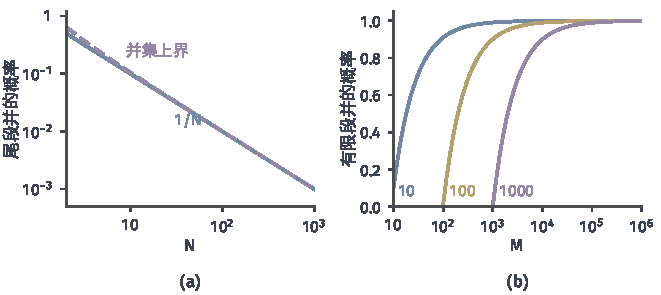
\includegraphics[width=112mm]{figures/07-probability/03-probability-limits/matplotlib/rvconv-bc-unions/figure.pdf}
 \caption{独立事件$A_n$尾段并的精确概率。(a)$\mathbb{P}(A_n)=1/n^{2}$：$\mathbb{P}(\bigcup_{n\geq N}A_n)=1/N$（蓝线）与并集上界$\sum_{n\geq N}n^{-2}$（紫色虚线），双对数坐标。(b)$\mathbb{P}(A_n)=1/n$：$\mathbb{P}(\bigcup_{n=N}^{M}A_n)=1-(N-1)/M$随$M$的变化，曲线旁的数字是起点$N$。}
 \label{fig:rvconv-bc-unions}
\end{BookInlineFigure}

图~\ref{fig:rvconv-bern-paths}从样本记录的角度看同一件事，画的是前$n$项中发生的次数$C_n=\sum_{k\leq n}\xi_k$。$p_n=1/n$时，计数在对数横轴上持续上升，期望是调和数$H_n\approx\ln n+0.577$，没有上限。$p_n=1/n^{2}$时，计数很早就停住，$10^{5}$项里只发生一两次。

\begin{BookInlineFigure}
 \centering
 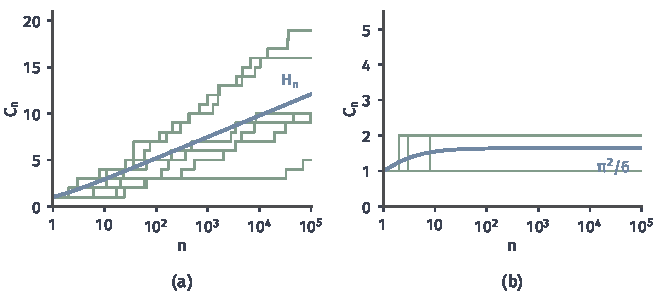
\includegraphics[width=112mm]{figures/07-probability/03-probability-limits/matplotlib/rvconv-bern-paths/figure.pdf}
 \caption{独立示性变量的累计发生次数$C_n=\sum_{k\leq n}\xi_k$，六条模拟记录（绿色，种子$2026$），横轴为对数刻度，$n\leq10^{5}$。蓝线是期望$\mathbb{E}[C_n]=\sum_{k\leq n}p_k$。(a)$p_n=1/n$，期望为调和数$H_n$，趋于无穷。(b)$p_n=1/n^{2}$，期望趋于$\pi^{2}/6\approx1.645$。}
 \label{fig:rvconv-bern-paths}
\end{BookInlineFigure}

两个引理合起来，对独立示性变量给出完整的回答：$\xi_n\xrightarrow{\mathrm{a.s.}}0$当且仅当$\sum_np_n<\infty$，而$\xi_n\xrightarrow{\mathbb{P}}0$当且仅当$p_n\to0$。$p_n\to0$但$\sum_np_n=\infty$的情形，例如$p_n=1/n$或$1/\sqrt{n}$，正好落在两者之间。它们还说明，独立事件的无穷多次发生只有两种可能：概率为$0$或为$1$。

\paragraph{去掉独立条件}
第二个引理的独立条件不能省略。取同一个事件重复：$A_n=A$对一切$n$成立，其中$0<\mathbb{P}(A)<1$。这时$\sum_n\mathbb{P}(A_n)=\infty$，但
\[
 \limsup_{n\to\infty}A_n=A,\qquad \mathbb{P}\Bigl(\limsup_{n\to\infty}A_n\Bigr)=\mathbb{P}(A)\in(0,1) .
\]
各项完全相关：在$A$上每次都发生，在$A$外从不发生。

依赖还可以把概率压到零。取$A_n=\{U<1/n\}$，$\sum_n1/n=\infty$，但这些事件递减，
\[
 \limsup_{n\to\infty}A_n=\bigcap_{n}\{U<1/n\}=\{U\leq0\},
\]
它的概率为零。所以概率发散时，没有独立性就什么也推不出：无穷多次发生的概率可以是$0$与$1$之间的任何值。第一个引理则对任何依赖结构都成立，这是两个方向在条件上的根本不对称。

\subsection{子列刻画}
\label{sec:rvconv-subsequence}

依概率收敛推不出几乎必然收敛，缺的是对整列的控制。但如果只看一部分项，跳过中间的项，超差概率就可能加起来有限。这是本小节的出发点：从依概率收敛的列中总能挑出几乎必然收敛的子列。

\begin{theorem}[几乎必然收敛的子列]
\label{thm:rvconv-subsequence}
若$X_n\xrightarrow{\mathbb{P}}X$，则存在子列$n_1<n_2<\cdots$，使$X_{n_k}\xrightarrow{\mathrm{a.s.}}X$。
\end{theorem}

\begin{proof}
由依概率收敛，对每个$k$，存在$N_k$使$n\geq N_k$时$\mathbb{P}(\lvert X_n-X\rvert>2^{-k})\leq2^{-k}$。递归地取$n_k\geq N_k$且$n_k>n_{k-1}$，令
\[
 E_k=\bigl\{\lvert X_{n_k}-X\rvert>2^{-k}\bigr\},\qquad \mathbb{P}(E_k)\leq2^{-k} .
\]

$\sum_k2^{-k}=1<\infty$，由引理~\ref{lem:rvconv-borel-cantelli}，$\mathbb{P}(\limsup_kE_k)=0$。对不在这个零概率事件中的$\omega$，存在$K(\omega)$，使$k\geq K(\omega)$时$\omega\notin E_k$，即
\[
 \lvert X_{n_k}(\omega)-X(\omega)\rvert\leq2^{-k},\qquad k\geq K(\omega) .
\]
右边趋于零，所以$X_{n_k}(\omega)\to X(\omega)$。
\end{proof}

阈值$2^{-k}$随$k$缩小，所以一个零概率例外集就同时照顾了所有精度，不需要再对$\varepsilon$取并。挑选子列的作用是让超差概率快速下降到可以求和，原列的超差概率可能下降得太慢。

\paragraph{移动区块的子列}
$B_n$依概率收敛到$0$，按定理应有几乎必然收敛的子列。每层取第一段即可：$n_k=k(k-1)/2+1$，
\[
 B_{n_k}=\mathbf{1}_{\{U<1/k\}} .
\]
对$U(\omega)>0$，$k>1/U(\omega)$以后$B_{n_k}(\omega)=0$，所以$B_{n_k}\xrightarrow{\mathrm{a.s.}}0$。图~\ref{fig:rvconv-subsequence}画出两条记录：原列在每层都碰到一次$1$，子列从某层起恒为零，而“某层”随记录改变。

\begin{BookInlineFigure}
 \centering
 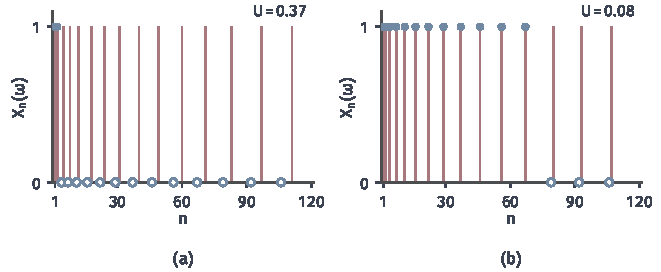
\includegraphics[width=112mm]{figures/07-probability/03-probability-limits/matplotlib/rvconv-subsequence/figure.pdf}
 \caption{移动区块的几乎必然收敛子列。红色竖线是原列$B_n(\omega)$取$1$的项，$n\leq120$；蓝点是子列$B_{n_k}=\mathbf{1}_{\{U<1/k\}}$（每层第一段）的取值，实心为$1$，空心为$0$。(a)$U=0.37$：子列只在$k=1,2$取$1$。(b)$U=0.08$：子列在$k\leq12$取$1$，此后恒为$0$。}
 \label{fig:rvconv-subsequence}
\end{BookInlineFigure}

这个子列的超差概率$1/k$加起来是发散的，它却几乎必然收敛：事件$\{U<1/k\}$递减，不独立。Borel–Cantelli引理是充分条件而不是必要条件。若按定理证明的办法挑选，会取到$k=2^{m}$那些层的第一段，超差概率$2^{-m}$可以求和。

\paragraph{独立示性变量的子列}
$p_n=1/n$时整列$\xi_n$不几乎必然收敛，但子列$n_k=k^{2}$的超差概率是$1/k^{2}$，可以求和。由引理~\ref{lem:rvconv-borel-cantelli}，$\xi_{k^{2}}\xrightarrow{\mathrm{a.s.}}0$。整列在几乎每条记录上无穷多次取$1$，但这些$1$几乎都落在跳过的项上。

\paragraph{完整的刻画}
一个几乎必然收敛的子列只是依概率收敛的一个推论，不足以反推整列依概率收敛。例如$X_{2m}=0$，$X_{2m-1}=\mathbf{1}_{\{U<1/2\}}$：偶数项的子列恒为零，而奇数项的超差概率恒为$1/2$，整列不依概率收敛到$0$。要刻画依概率收敛，必须对每一个子列都提出要求。

\begin{theorem}[依概率收敛的子列刻画]
\label{thm:rvconv-subsequence-criterion}
$X_n\xrightarrow{\mathbb{P}}X$当且仅当：对$(X_n)$的每个子列$(X_{n_k})$，都存在进一步的子列$(X_{n_{k_j}})$，使$X_{n_{k_j}}\xrightarrow{\mathrm{a.s.}}X$。
\end{theorem}

\begin{proof}
必要性。依概率收敛列的每个子列仍依概率收敛到$X$，对这个子列用定理~\ref{thm:rvconv-subsequence}即可。

充分性用反证法。若$X_n$不依概率收敛到$X$，则存在$\varepsilon>0$、$\delta>0$和子列$(n_k)$，使
\[
 \mathbb{P}\bigl(\lvert X_{n_k}-X\rvert>\varepsilon\bigr)\geq\delta,\qquad k=1,2,\dots
\]
按假设，它有进一步的子列几乎必然收敛到$X$，由定理~\ref{thm:rvconv-implications}也依概率收敛到$X$，其超差概率趋于零，与上式矛盾。
\end{proof}

前一个例子中，奇数项组成的子列没有任何进一步的子列收敛到$0$，所以条件不满足，这与整列不收敛一致。

\paragraph{几乎必然收敛没有这样的刻画}
移动区块满足定理~\ref{thm:rvconv-subsequence-criterion}中的条件：每个子列仍依概率收敛到$0$，因而有几乎必然收敛的进一步子列。但整列不几乎必然收敛。所以“每个子列都有收敛到$X$的进一步子列”这一条件，对几乎必然收敛不是充分的。

对由拓扑或距离定义的收敛，这一条件总是充分的：若$x_n\not\to x$，就有$x$的一个邻域和一个整个落在邻域外的子列，这个子列的任何进一步子列都不收敛到$x$。因此不存在一种距离，使随机变量按这种距离收敛恰好是几乎必然收敛。

依概率收敛则可以用一个平均量描述。对$0<\varepsilon\leq1$，把误差在$\varepsilon$处分开，并分别用$\min\{\lvert x\rvert,1\}\leq\varepsilon$（当$\lvert x\rvert\leq\varepsilon$）与$\min\{\lvert x\rvert,1\}\leq1$估计，再对超差事件用Markov不等式，得到
\[
 \varepsilon\,\mathbb{P}\bigl(\lvert X_n-X\rvert>\varepsilon\bigr)\leq\mathbb{E}\bigl[\min\{\lvert X_n-X\rvert,1\}\bigr]\leq\varepsilon+\mathbb{P}\bigl(\lvert X_n-X\rvert>\varepsilon\bigr) .
\]
所以$X_n\xrightarrow{\mathbb{P}}X$当且仅当$\mathbb{E}[\min\{\lvert X_n-X\rvert,1\}]\to0$。截去大于$1$的部分，是为了让稀有大值不影响这个平均，它衡量的只是“超差的机会”。

\paragraph{连续映射}
子列刻画的一个直接用途是传递依概率收敛。设$g:\mathbb{R}\to\mathbb{R}$连续，$X_n\xrightarrow{\mathbb{P}}X$，要证$g(X_n)\xrightarrow{\mathbb{P}}g(X)$。直接估计$\mathbb{P}(\lvert g(X_n)-g(X)\rvert>\varepsilon)$需要$g$的一致连续性，而$g$在整条实轴上未必一致连续。

用子列刻画则只需逐点的连续性。任取一个子列，它有进一步的子列几乎必然收敛到$X$；在这个子列上，对收敛的记录$\omega$，由$g$的连续性，$g(X_{n_{k_j}}(\omega))\to g(X(\omega))$，即$g(X_{n_{k_j}})\xrightarrow{\mathrm{a.s.}}g(X)$。由定理~\ref{thm:rvconv-subsequence-criterion}，$g(X_n)\xrightarrow{\mathbb{P}}g(X)$。例如$X_n\xrightarrow{\mathbb{P}}X$推出$X_n^{2}\xrightarrow{\mathbb{P}}X^{2}$。


\section{期望与极限}
\label{sec:rvconv-expectation-limits}

$Y_n=n\,\mathbf{1}_{\{U<1/n\}}$几乎必然收敛到$0$，期望却恒为$1$：
\[
 \lim_{n\to\infty}\mathbb{E}[Y_n]=1\neq0=\mathbb{E}\Bigl[\lim_{n\to\infty}Y_n\Bigr] .
\]
随机变量趋近目标，少量的大取值仍然可以左右期望。期望与极限什么时候可以交换？本节依次研究三类条件给出的保证：单调的符号结构、一个共同的可积上界，以及对整族变量尾部的统一控制。

积分的单调收敛定理、Fatou引理与支配收敛定理已经在一般测度空间上证明，可参考\BookChapterRef{chap:integration}{卷四第6章“积分”}。期望就是概率测度下的积分，这些定理可以直接使用。本节的重点是解释每个条件在随机误差中起什么作用，以及去掉它时期望会怎样出错。

\subsection{单调收敛}
\label{sec:rvconv-monotone}

最容易的情形是变量单调增加。非负的量只增不减，取极限时不会丢掉已经累积的部分。

\begin{theorem}[单调收敛定理]
\label{thm:rvconv-monotone}
设随机变量$0\leq X_1\leq X_2\leq\cdots$几乎必然成立，且$X_n\xrightarrow{\mathrm{a.s.}}X$。则
\begin{equation}
 \lim_{n\to\infty}\mathbb{E}[X_n]=\mathbb{E}[X] ,
 \label{eq:rvconv-monotone}
\end{equation}
两边可以同时为$+\infty$。
\end{theorem}

这是卷四单调收敛定理在概率空间上的写法：在一个零概率事件之外，$X_n$逐点递增到$X$，把这个事件上的值改为零不改变任何期望。结论不要求$X$可积，极限期望允许是$+\infty$。

\paragraph{计数与Borel–Cantelli引理}
单调收敛最常见的来源是非负项的累计。设$A_1,A_2,\dots$是事件，前$n$个事件中发生的个数与总发生次数分别是
\[
 N_n=\sum_{k=1}^{n}\mathbf{1}_{A_k},\qquad N=\sum_{k=1}^{\infty}\mathbf{1}_{A_k} .
\]
$N_n$在每条记录上递增到$N$，$N$可以取$+\infty$。由期望的线性性，$\mathbb{E}[N_n]=\sum_{k\leq n}\mathbb{P}(A_k)$；再由定理~\ref{thm:rvconv-monotone}，
\begin{equation}
 \mathbb{E}\Bigl[\sum_{k=1}^{\infty}\mathbf{1}_{A_k}\Bigr]=\sum_{k=1}^{\infty}\mathbb{P}(A_k) .
 \label{eq:rvconv-count-mean}
\end{equation}

这给出Borel–Cantelli引理的另一个证明。若$\sum_k\mathbb{P}(A_k)<\infty$，则$\mathbb{E}[N]<\infty$；期望有限的非负随机变量几乎必然有限（否则在正概率事件上取$+\infty$，期望也是$+\infty$），所以几乎每条记录上只有有限个事件发生。“概率可和”就是“平均发生次数有限”。

\paragraph{极限期望可以是无穷}
反方向不成立：平均次数无穷，次数本身仍可能处处有限。取$A_k=\{U<1/k\}$。对给定的$U(\omega)>0$，$U<1/k$当且仅当$k<1/U$，所以
\[
 N_n=\min\Bigl\{n,\ \Bigl\lceil\frac1U\Bigr\rceil-1\Bigr\},\qquad N=\Bigl\lceil\frac1U\Bigr\rceil-1 .
\]
$N$在$U>0$时有限，即几乎必然有限。它的期望却是
\[
 \mathbb{E}[N]=\lim_{n\to\infty}\mathbb{E}[N_n]=\lim_{n\to\infty}\sum_{k=1}^{n}\frac1k=+\infty .
\]

\begin{BookInlineFigure}
 \centering
 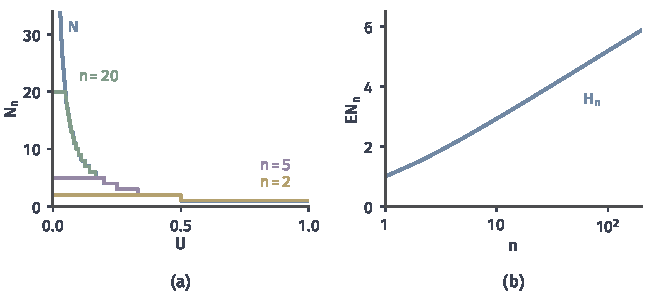
\includegraphics[width=112mm]{figures/07-probability/03-probability-limits/matplotlib/rvconv-monotone-count/figure.pdf}
 \caption{递增的计数变量$N_n=\sum_{k\leq n}\mathbf{1}_{\{U<1/k\}}$。(a)$N_n$作为$U$的函数，$n=2,5,20$（黄、紫、绿），蓝色台阶是极限$N=\lceil1/U\rceil-1$；各条台阶在$N\leq n$处与极限重合，只在$U$接近$0$处被截平。(b)$\mathbb{E}[N_n]=H_n=\sum_{k\leq n}1/k$，横轴为对数刻度。}
 \label{fig:rvconv-monotone-count}
\end{BookInlineFigure}

图~\ref{fig:rvconv-monotone-count}(a)中，$N_n$是极限$N$在高度$n$处的截平，截平的部分只在$U<1/n$这一小段上。随着$n$增大，截平的位置抬高，$N_n$下方的面积$H_n$一点一点地逼近$N$下方的面积。$N$在$U\to0$时像$1/U$那样增长，面积发散，(b)中$H_n\approx\ln n+0.577$随之无界增长。单调收敛定理正确地给出$\mathbb{E}[N]=+\infty$，它不需要极限可积。

\paragraph{单调性为何保留全部质量}
递增列不会丢掉期望的原因可以这样理解：每个$X_n$都在极限$X$的下方，且越来越贴近它。$X$的期望由它在各处的取值累积而成，任何一块有贡献的区域，迟早都会被$X_n$从下方填满，不存在“先出现、后消失”的贡献。

仅有非负性不够。$Y_n$非负且几乎必然趋于$0$，但不单调：$Y_n$在$\{U<1/n\}$上取$n$，在$Y_{n+1}$时这一块的大部分归零，又在更窄的$\{U<1/(n+1)\}$上取更大的值。图~\ref{fig:rvconv-spike-mass}在取值的数轴上画出它的分布：$Y_n$把质量$1/n$放在远处的$n$上，这一小块质量对均值的贡献恒为$n\cdot1/n=1$。随着$n$增大，这块质量越来越小、越来越远，极限中它消失了，它对均值的贡献却始终在。

\begin{BookInlineFigure}
 \centering
 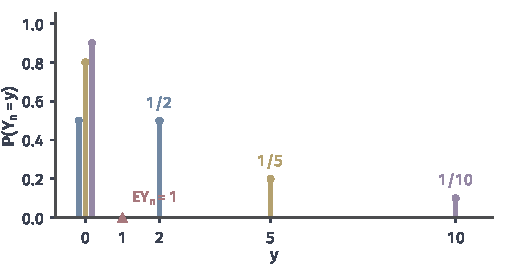
\includegraphics[width=86mm]{figures/07-probability/03-probability-limits/matplotlib/rvconv-spike-mass/figure.pdf}
 \caption{$Y_n=n\,\mathbf{1}_{\{U<1/n\}}$的分布，$n=2,5,10$（蓝、黄、紫）：质量$1-1/n$在$0$，质量$1/n$在$n$（$0$处的柱略微错开）。红三角是均值$\mathbb{E}[Y_n]=1$，对每个$n$都相同。}
 \label{fig:rvconv-spike-mass}
\end{BookInlineFigure}

\paragraph{递减的情形}
对递减列，单调性还需要配合可积性。若$X_n\geq0$递减到$X$且$\mathbb{E}[X_1]<\infty$，则$X_1-X_n$非负递增到$X_1-X$，对它用定理~\ref{thm:rvconv-monotone}，再从两边减去有限的$\mathbb{E}[X_1]$，得到$\mathbb{E}[X_n]\downarrow\mathbb{E}[X]$。

$\mathbb{E}[X_1]<\infty$不能省。取$X_n=U^{-1}\mathbf{1}_{\{U<1/n\}}$，它在$U>0$时递减到$0$，但对每个$n$，
\[
 \mathbb{E}[X_n]=\int_0^{1/n}\frac{\mathrm{d}u}{u}=+\infty .
\]
极限的期望是$0$，各项的期望都是$+\infty$。无穷减无穷没有意义，单调收敛定理只能用于递增的方向。

\subsection{Fatou引理}
\label{sec:rvconv-fatou}

不单调的非负列中，期望可以在极限里丢失，$Y_n$就是例子。但丢失只有一个方向：非负变量的质量可以逃到远处而消失，不能凭空产生。Fatou引理把这个单向的控制写成不等式。

\begin{theorem}[Fatou引理]
\label{thm:rvconv-fatou}
设随机变量$X_n\geq0$几乎必然成立，则
\begin{equation}
 \mathbb{E}\Bigl[\liminf_{n\to\infty}X_n\Bigr]\leq\liminf_{n\to\infty}\mathbb{E}[X_n] .
 \label{eq:rvconv-fatou}
\end{equation}
\end{theorem}

\begin{proof}
令$G_n=\inf_{k\geq n}X_k$。它非负，随$n$递增，极限是$\liminf_nX_n$。由定理~\ref{thm:rvconv-monotone}，
\[
 \mathbb{E}[G_n]\to\mathbb{E}\Bigl[\liminf_{n\to\infty}X_n\Bigr] .
\]

另一方面，对每个$k\geq n$都有$G_n\leq X_k$，所以$\mathbb{E}[G_n]\leq\mathbb{E}[X_k]$，对$k\geq n$取下确界，得到
\[
 \mathbb{E}[G_n]\leq\inf_{k\geq n}\mathbb{E}[X_k] .
\]
令$n\to\infty$，左边趋于式~\eqref{eq:rvconv-fatou}的左边，右边趋于它的右边。
\end{proof}

证明把一般的列换成它的尾部下确界，后者是递增的，于是可以用单调收敛。下确界只会比每一项都小，这就是不等式只有一个方向的来源。

\paragraph{严格不等号}
对$Y_n$，每条$U>0$的记录上$Y_n\to0$，所以式~\eqref{eq:rvconv-fatou}的两边是
\[
 \mathbb{E}\Bigl[\liminf_{n\to\infty}Y_n\Bigr]=0,\qquad \liminf_{n\to\infty}\mathbb{E}[Y_n]=1 .
\]
不等号严格成立，差额$1$正是逃到远处的那一块质量的贡献。概率越来越小、幅值越来越大的变量，总可以这样让极限的期望小于期望的极限。

\paragraph{非负性的作用}
把$Y_n$换成$-Y_n$，变量非正，几乎必然趋于$0$，而$\mathbb{E}[-Y_n]=-1$。这时
\[
 \mathbb{E}\Bigl[\liminf_{n\to\infty}(-Y_n)\Bigr]=0>-1=\liminf_{n\to\infty}\mathbb{E}[-Y_n] ,
\]
不等式反向。负的大值逃到远处时，带走的是负的贡献，极限的期望反而变大。所以Fatou引理需要下方的控制：非负，或者更一般地$X_n\geq-G$且$\mathbb{E}[G]<\infty$（对$X_n+G$用引理）。

\paragraph{极限的可积性}
Fatou引理最常用的形式是给极限的期望一个上界。若$X_n\xrightarrow{\mathrm{a.s.}}X$且$\sup_n\mathbb{E}[\lvert X_n\rvert]\leq C$，对$\lvert X_n\rvert$用式~\eqref{eq:rvconv-fatou}，得到
\begin{equation}
 \mathbb{E}[\lvert X\rvert]\leq\liminf_{n\to\infty}\mathbb{E}[\lvert X_n\rvert]\leq C .
 \label{eq:rvconv-fatou-bound}
\end{equation}
各项的平均绝对值一致有界时，极限必然可积。它只给出不等式，并不说明$\mathbb{E}[X_n]$收敛到$\mathbb{E}[X]$：$Y_n$满足$C=1$，极限的期望$0$严格小于$1$。

\subsection{支配收敛}
\label{sec:rvconv-dominated}

要得到等式，需要阻止质量逃逸。最直接的办法是给整列找一个共同的上界，并要求这个上界本身可积：所有变量都被关在同一个“有限面积”的笼子里。

\begin{theorem}[支配收敛定理]
\label{thm:rvconv-dominated}
设$X_n\xrightarrow{\mathrm{a.s.}}X$，并存在随机变量$G$，使$\mathbb{E}[G]<\infty$且对每个$n$都有$\lvert X_n\rvert\leq G$几乎必然成立。则$X$可积，且
\begin{equation}
 \lim_{n\to\infty}\mathbb{E}\bigl[\lvert X_n-X\rvert\bigr]=0,\qquad \lim_{n\to\infty}\mathbb{E}[X_n]=\mathbb{E}[X] .
 \label{eq:rvconv-dominated}
\end{equation}
\end{theorem}

\begin{proof}
取极限得$\lvert X\rvert\leq G$几乎必然，所以$X$可积，并且$\lvert X_n-X\rvert\leq2G$。于是$2G-\lvert X_n-X\rvert$非负，几乎必然趋于$2G$。由Fatou引理，
\[
 \mathbb{E}[2G]\leq\liminf_{n\to\infty}\mathbb{E}\bigl[2G-\lvert X_n-X\rvert\bigr]=\mathbb{E}[2G]-\limsup_{n\to\infty}\mathbb{E}\bigl[\lvert X_n-X\rvert\bigr] .
\]

$\mathbb{E}[2G]$有限，可以从两边消去，得到$\limsup_n\mathbb{E}[\lvert X_n-X\rvert]\leq0$，即平均绝对误差趋于零。最后，
\[
 \bigl\lvert\mathbb{E}[X_n]-\mathbb{E}[X]\bigr\rvert\leq\mathbb{E}\bigl[\lvert X_n-X\rvert\bigr]\to0 .
\]
\end{proof}

证明的关键是把误差$\lvert X_n-X\rvert$翻成$2G$减去它，后者非负，Fatou引理就从“只能变小”的单向控制变成了对误差的控制。可积性$\mathbb{E}[G]<\infty$用在消去$\mathbb{E}[2G]$这一步。

\paragraph{有界收敛}
概率空间的总质量为一，常数是可积的。所以若$\lvert X_n\rvert\leq c$对某个常数$c$成立，支配条件自动满足，这称为\term{有界收敛定理}（bounded convergence theorem）。累计最大值满足$0\leq M_n\leq1$，于是
\[
 \mathbb{E}[M_n]=\frac{n}{n+1}\to1=\mathbb{E}[1] .
\]
在一般测度空间上，常数在总测度无限时不可积，有界收敛不能这样直接得到。

\paragraph{依概率收敛下的支配收敛}
定理中的几乎必然收敛可以减弱为依概率收敛。设$X_n\xrightarrow{\mathbb{P}}X$，$\lvert X_n\rvert\leq G$，$\mathbb{E}[G]<\infty$，记$a_n=\mathbb{E}[\lvert X_n-X\rvert]$。由定理~\ref{thm:rvconv-subsequence}，有子列几乎必然收敛到$X$，取极限得$\lvert X\rvert\leq G$，$X$可积。

再看数列$(a_n)$的任意子列。由定理~\ref{thm:rvconv-subsequence-criterion}，它有进一步的子列使$X_n$几乎必然收敛到$X$，对这个子列用定理~\ref{thm:rvconv-dominated}，相应的$a_n$趋于零。一个实数列的每个子列都有趋于零的进一步子列，整个数列就趋于零，所以$a_n\to0$。

\paragraph{共同上界与包络}
$Y_n$为什么不满足定理？任何共同上界$G$都不小于包络$\sup_nY_n$。对$U(\omega)>0$，$Y_n(\omega)=n$当且仅当$n<1/U(\omega)$，所以包络就是第~\ref{sec:rvconv-monotone}小节的计数变量：
\[
 \sup_nY_n=\Bigl\lceil\frac1U\Bigr\rceil-1=N,\qquad \mathbb{E}[N]=+\infty .
\]
包络不可积，任何共同上界也不可积，支配收敛定理不适用，结论也确实不成立。

$Z_n=\sqrt n\,\mathbf{1}_{\{U<1/n\}}$的包络是$\sqrt N$。$N=n$当且仅当$1/(n+1)\leq U<1/n$，概率为$1/(n(n+1))$，所以
\[
 \mathbb{E}\bigl[\sqrt N\bigr]=\sum_{n=1}^{\infty}\frac{\sqrt n}{n(n+1)}=\sum_{n=1}^{\infty}\frac{1}{\sqrt n\,(n+1)}\approx1.860 .
\]
包络可积，支配收敛定理给出$\mathbb{E}[Z_n]\to0$，与直接计算的$n^{-1/2}$一致。

\begin{BookInlineFigure}
 \centering
 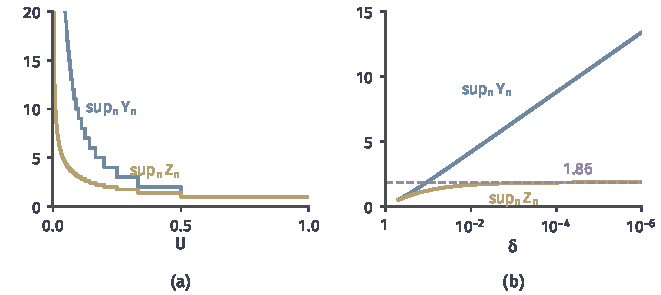
\includegraphics[width=112mm]{figures/07-probability/03-probability-limits/matplotlib/rvconv-envelope/figure.pdf}
 \caption{两族稀有大值的包络。(a)$\sup_nY_n=\lceil1/U\rceil-1$（蓝）与$\sup_nZ_n=\sqrt{\lceil1/U\rceil-1}$（黄）作为$U$的函数。(b)从$\delta$到$1$的积分随$\delta\to0$的变化，横轴为对数刻度且向右递减：蓝线按$\ln(1/\delta)$无界增长，黄线趋于$\mathbb{E}[\sqrt N]\approx1.86$（紫色虚线）。}
 \label{fig:rvconv-envelope}
\end{BookInlineFigure}

图~\ref{fig:rvconv-envelope}比较两个包络。两者在$U\to0$时都趋于无穷，差别在于增长的快慢：$\sup_nY_n$像$1/U$，下方面积发散；$\sup_nZ_n$像$U^{-1/2}$，下方面积有限。共同上界控制的不是单个变量，而是整族变量在稀有区域上能取到的最大值。

\paragraph{共同上界控制了什么}
共同可积上界的作用可以写成一个统一的尾部估计。若$\lvert X_n\rvert\leq G$，则$\{\lvert X_n\rvert>M\}\subseteq\{G>M\}$，在这个事件上$\lvert X_n\rvert\leq G$，所以
\begin{equation}
 \sup_n\mathbb{E}\bigl[\lvert X_n\rvert\,\mathbf{1}_{\{\lvert X_n\rvert>M\}}\bigr]\leq\mathbb{E}\bigl[G\,\mathbf{1}_{\{G>M\}}\bigr] .
 \label{eq:rvconv-envelope-tail}
\end{equation}
右边是单个可积变量的尾部贡献，$M\to\infty$时由支配收敛趋于零。共同上界真正做到的，是让整族变量在大取值处的贡献一起变小。下一小节把这一点单独拿出来作为条件。

\subsection{一致可积性}
\label{sec:rvconv-uniform-integrability}

$Y_n$的问题是平均被越来越稀有的大值维持着。要排除这种情形，应当要求大取值区域上的贡献对整族变量一致地小，而不必要求有一个共同的上界。

\begin{definition}[一致可积]
\label{def:rvconv-ui}
设$\{X_i:i\in I\}$是一族可积随机变量。若
\begin{equation}
 \lim_{M\to\infty}\ \sup_{i\in I}\ \mathbb{E}\bigl[\lvert X_i\rvert\,\mathbf{1}_{\{\lvert X_i\rvert>M\}}\bigr]=0 ,
 \label{eq:rvconv-ui}
\end{equation}
称这族变量\term{一致可积}（uniformly integrable）。
\end{definition}

单个可积变量$X$总满足这个条件：$\lvert X\rvert\mathbf{1}_{\{\lvert X\rvert>M\}}$被$\lvert X\rvert$控制，且在$\lvert X\rvert<\infty$处随$M\to\infty$趋于零，由支配收敛定理，它的期望趋于零。有限个可积变量也一致可积，对每个变量分别取$M$再取最大的那个即可。一致可积性的内容在于无穷多个变量同时满足，即同一个$M$对整族有效。

\paragraph{贯穿例子}
$Y_n$不一致可积。对任意$M$，当$n>M$时$\{Y_n>M\}=\{U<1/n\}$，所以
\[
 \mathbb{E}\bigl[Y_n\mathbf{1}_{\{Y_n>M\}}\bigr]=n\cdot\frac1n=1,\qquad
 \sup_n\mathbb{E}\bigl[Y_n\mathbf{1}_{\{Y_n>M\}}\bigr]=1 .
\]
无论阈值抬多高，总有某个$Y_n$把全部平均放在阈值之上。

$Z_n$一致可积。只有$\sqrt n>M$时$\{Z_n>M\}$才非空，此时它的贡献是$\sqrt n\cdot1/n=1/\sqrt n<1/M$，所以
\[
 \sup_n\mathbb{E}\bigl[Z_n\mathbf{1}_{\{Z_n>M\}}\bigr]\leq\frac1M\to0 .
\]
累计最大值在$[0,1]$中取值，$M\geq1$时贡献为零。图~\ref{fig:rvconv-ui-tails}画出三族的上确界随$M$的变化。

\begin{BookInlineFigure}
 \centering
 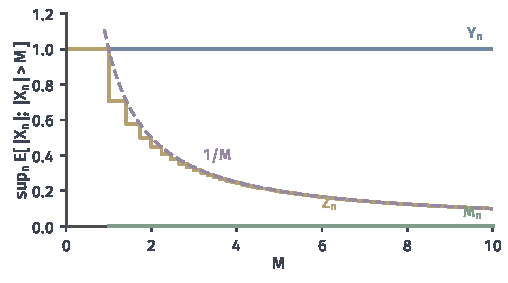
\includegraphics[width=86mm]{figures/07-probability/03-probability-limits/matplotlib/rvconv-ui-tails/figure.pdf}
 \caption{大取值区域上的一致贡献$\sup_n\mathbb{E}[\lvert X_n\rvert;\lvert X_n\rvert>M]$随阈值$M$的变化。蓝线：$Y_n$，恒为$1$，不一致可积。黄色台阶：$Z_n$，等于$1/\sqrt{\lfloor M^{2}\rfloor+1}$。紫色虚线：二阶矩给出的上界$\sup_n\mathbb{E}[Z_n^{2}]/M=1/M$。绿线：$M_n$，$M\geq1$时为零。}
 \label{fig:rvconv-ui-tails}
\end{BookInlineFigure}

\paragraph{判据}
直接验证式~\eqref{eq:rvconv-ui}往往不方便。下面三条比较常用的条件说明：共同可积上界和高于一阶的一致矩界都足够，而一阶矩一致有界本身不够。

\begin{theorem}[一致可积的充分条件]
\label{thm:rvconv-ui-criteria}
设$\{X_i:i\in I\}$是一族随机变量。
\begin{enumerate}
 \item 若存在$G$，$\mathbb{E}[G]<\infty$，使$\lvert X_i\rvert\leq G$对每个$i$几乎必然成立，则这族变量一致可积。
 \item 若存在$p>1$与$K<\infty$，使$\mathbb{E}[\lvert X_i\rvert^{p}]\leq K$对每个$i$成立，则这族变量一致可积，且
 \begin{equation}
  \sup_{i\in I}\mathbb{E}\bigl[\lvert X_i\rvert\,\mathbf{1}_{\{\lvert X_i\rvert>M\}}\bigr]\leq\frac{K}{M^{p-1}} .
  \label{eq:rvconv-ui-moment}
 \end{equation}
 \item 仅有$\sup_i\mathbb{E}[\lvert X_i\rvert]<\infty$不能推出一致可积。
\end{enumerate}
\end{theorem}

\begin{proof}
第1条即式~\eqref{eq:rvconv-envelope-tail}。

第2条。在$\{\lvert X_i\rvert>M\}$上，$\lvert X_i\rvert^{1-p}<M^{1-p}$，所以
\[
 \lvert X_i\rvert=\lvert X_i\rvert^{p}\cdot\lvert X_i\rvert^{1-p}\leq\frac{\lvert X_i\rvert^{p}}{M^{p-1}} .
\]
乘以$\mathbf{1}_{\{\lvert X_i\rvert>M\}}$再取期望，右边的期望不超过$\mathbb{E}[\lvert X_i\rvert^{p}]\leq K$，即得式~\eqref{eq:rvconv-ui-moment}。$p>1$保证右边随$M\to\infty$趋于零。

第3条。$Y_n$满足$\mathbb{E}[Y_n]=1$，但上面已算出它不一致可积。
\end{proof}

第2条中$p>1$是关键。$p$阶矩有界意味着大取值必须付出更高的代价：取值为$y$的部分在$p$阶矩中按$y^{p}$计入，在平均中只按$y$计入，所以平均的尾部被$p$阶矩以$M^{1-p}$的速度压住。$p=1$时这个比例是$1$，没有压缩，$Y_n$就钻了这个空子。$Z_n$满足$\mathbb{E}[Z_n^{2}]=1$，第2条给出上界$1/M$，正是图~\ref{fig:rvconv-ui-tails}中的紫色虚线。

同样的论证适用于任何增长快于线性的函数。若$\varphi\geq0$满足$\varphi(t)/t\to\infty$（$t\to\infty$），且$\sup_i\mathbb{E}[\varphi(\lvert X_i\rvert)]\leq K$，则在$\{\lvert X_i\rvert>M\}$上
\[
 \lvert X_i\rvert=\varphi(\lvert X_i\rvert)\cdot\frac{\lvert X_i\rvert}{\varphi(\lvert X_i\rvert)}\leq\varphi(\lvert X_i\rvert)\,\sup_{t>M}\frac{t}{\varphi(t)} ,
\]
于是尾部贡献不超过$K\sup_{t>M}t/\varphi(t)$，它随$M\to\infty$趋于零。例如$\varphi(t)=t\ln(1+t)$，它只比一阶矩多一个对数因子。反过来，每个一致可积族都存在这样的$\varphi$，这一方向的证明需要构造$\varphi$，篇幅较长，读者可查阅~\scite{math-kallenberg2021probability}。

\paragraph{小事件上的一致控制}
一致可积还有一个等价的说法：平均有界，并且在概率很小的事件上，整族变量的贡献一致地小。它把“大取值”换成了“小事件”，在证明中更方便。

\begin{lemma}[一致可积的等价刻画]
\label{lem:rvconv-ui-small-sets}
一族随机变量$\{X_i:i\in I\}$一致可积，当且仅当以下两条同时成立：
\begin{enumerate}
 \item $\sup_{i\in I}\mathbb{E}[\lvert X_i\rvert]<\infty$；
 \item 对每个$\eta>0$，存在$\delta>0$，使对每个满足$\mathbb{P}(A)<\delta$的事件$A$，
 \begin{equation}
  \sup_{i\in I}\mathbb{E}\bigl[\lvert X_i\rvert\,\mathbf{1}_{A}\bigr]<\eta .
  \label{eq:rvconv-ui-small-sets}
 \end{equation}
\end{enumerate}
\end{lemma}

\begin{proof}
必要性。把事件$A$按$\lvert X_i\rvert$是否超过$M$分成两块，第二块上$\lvert X_i\rvert\leq M$，所以
\[
 \mathbb{E}\bigl[\lvert X_i\rvert\,\mathbf{1}_{A}\bigr]\leq\mathbb{E}\bigl[\lvert X_i\rvert\,\mathbf{1}_{\{\lvert X_i\rvert>M\}}\bigr]+M\,\mathbb{P}(A) .
\]
给定$\eta>0$，先取$M$使第一项对所有$i$都小于$\eta/2$，再取$\delta=\eta/(2M)$，则$\mathbb{P}(A)<\delta$时左边小于$\eta$。取$A=\Omega$，第一项小于$\eta/2$，第二项是$M$，得到第1条。

充分性。记$C=\sup_i\mathbb{E}[\lvert X_i\rvert]$。由Markov不等式，
\[
 \mathbb{P}\bigl(\lvert X_i\rvert>M\bigr)\leq\frac{C}{M}\qquad\text{对每个 }i .
\]
给定$\eta$，取第2条中的$\delta$，再取$M>C/\delta$，则每个事件$\{\lvert X_i\rvert>M\}$的概率都小于$\delta$，由式~\eqref{eq:rvconv-ui-small-sets}，其上的贡献小于$\eta$，且对所有$i$同时成立。
\end{proof}

充分性中第1条不可缺：它保证事件$\{\lvert X_i\rvert>M\}$对整族一致地小，第2条才能用上。这个刻画说明，一致可积排除的正是“把平均藏在越来越小的事件里”。$Y_n$在概率$1/n$的事件上放下整份平均$1$，第2条对它不成立。

\subsection{\texorpdfstring{$L^{1}$}{L1}收敛的判据}
\label{sec:rvconv-l1-criterion}

现在可以回答本节开头的问题。依概率收敛缺的是尾部控制，一致可积恰好补上它，而且补得不多不少：在依概率收敛的前提下，$L^{1}$收敛与一致可积等价。

\begin{theorem}[Vitali收敛定理]
\label{thm:rvconv-vitali}
设$X_n\xrightarrow{\mathbb{P}}X$，且$\{X_n\}$一致可积。则$X$可积，且
\begin{equation}
 \lim_{n\to\infty}\mathbb{E}\bigl[\lvert X_n-X\rvert\bigr]=0,\qquad \lim_{n\to\infty}\mathbb{E}[X_n]=\mathbb{E}[X] .
 \label{eq:rvconv-vitali}
\end{equation}
\end{theorem}

这一结论称为\term{Vitali收敛定理}（Vitali convergence theorem）。卷四对有限测度空间的依测度收敛给出了一个按小区域估计的证明。这里换一种在概率论中更常用的写法：把每个变量截断成有界变量，有界部分用有界收敛，截掉的尾部用一致可积。对$M>0$，令
\[
 \varphi_M(x)=\max\{-M,\min\{x,M\}\} ,
\]
即把$x$限制在$[-M,M]$内。它满足两条性质：截断不会拉大两点的距离，截断误差只出现在阈值之外，
\[
 \lvert\varphi_M(x)-\varphi_M(y)\rvert\leq\lvert x-y\rvert,\qquad
 \lvert x-\varphi_M(x)\rvert\leq\lvert x\rvert\,\mathbf{1}_{\{\lvert x\rvert>M\}} .
\]
后一式左边等于$\max\{\lvert x\rvert-M,0\}$。

\begin{BookInlineFigure}
 \centering
 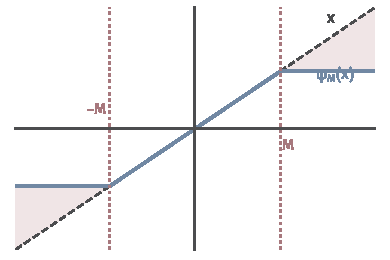
\includegraphics[width=66mm]{figures/07-probability/03-probability-limits/matplotlib/rvconv-truncation/figure.pdf}
 \caption{截断函数$\varphi_M$（蓝线，$M=2$）与恒等函数（灰色虚线）。两者只在$\lvert x\rvert>M$处不同，浅红区域的竖直高度就是截断误差$\lvert x-\varphi_M(x)\rvert=(\lvert x\rvert-M)^{+}$。}
 \label{fig:rvconv-truncation}
\end{BookInlineFigure}

图~\ref{fig:rvconv-truncation}画出截断误差的位置：它只出现在阈值之外，而一致可积说的正是阈值之外的贡献一致地小。

\begin{proof}
先证$X$可积。由引理~\ref{lem:rvconv-ui-small-sets}，$C=\sup_n\mathbb{E}[\lvert X_n\rvert]<\infty$。由定理~\ref{thm:rvconv-subsequence}，有子列$X_{n_k}\xrightarrow{\mathrm{a.s.}}X$，再由式~\eqref{eq:rvconv-fatou-bound}，$\mathbb{E}[\lvert X\rvert]\leq C$。

再估计误差。固定$M>0$，在$X_n$与$X$之间插入截断，由三角不等式，
\[
 \lvert X_n-X\rvert\leq\lvert X_n-\varphi_M(X_n)\rvert+\lvert\varphi_M(X_n)-\varphi_M(X)\rvert+\lvert\varphi_M(X)-X\rvert .
\]
取期望，逐项处理。

第一项是截掉的尾部，由截断误差的估计，
\[
 \mathbb{E}\bigl[\lvert X_n-\varphi_M(X_n)\rvert\bigr]\leq\tau(M),\qquad \tau(M)=\sup_k\mathbb{E}\bigl[\lvert X_k\rvert\,\mathbf{1}_{\{\lvert X_k\rvert>M\}}\bigr] .
\]
第三项同理不超过$\mathbb{E}[\lvert X\rvert\mathbf{1}_{\{\lvert X\rvert>M\}}]$。

第二项是有界部分。由$\varphi_M$的第一条性质，截断后的误差不超过原误差，所以$\varphi_M(X_n)\xrightarrow{\mathbb{P}}\varphi_M(X)$；同时它不超过$2M$。由依概率收敛下的有界收敛（第~\ref{sec:rvconv-dominated}小节），第二项的期望趋于零。于是
\[
 \limsup_{n\to\infty}\mathbb{E}\bigl[\lvert X_n-X\rvert\bigr]\leq\tau(M)+\mathbb{E}\bigl[\lvert X\rvert\,\mathbf{1}_{\{\lvert X\rvert>M\}}\bigr] .
\]

左边与$M$无关。令$M\to\infty$，第一项由一致可积趋于零，第二项因$X$可积而趋于零，所以平均绝对误差趋于零。期望的收敛与支配收敛定理的证明末尾相同。
\end{proof}

三个部分各有分工：依概率收敛只管有界的中间部分，一致可积管住所有$X_n$的尾部，$X$的可积性管住极限的尾部。缺了一致可积，第一项不能对所有$n$同时变小，$Y_n$就是这种情形：$\tau(M)=1$，误差停在$1$。

用贯穿例子核对。$Z_n\xrightarrow{\mathbb{P}}0$且一致可积，定理给出$\mathbb{E}[Z_n]\to0$，与直接计算的$n^{-1/2}$一致。移动区块与$\xi_n$都只取$0$和$1$，由第1条判据（$G=1$）一致可积，它们依概率收敛到$0$，所以也$L^{1}$收敛到$0$，与第~\ref{sec:rvconv-lp}小节的计算一致。

\paragraph{反方向}
$L^{1}$收敛的列一定一致可积，所以一致可积不只是充分条件。

\begin{theorem}[$L^{1}$收敛蕴含一致可积]
\label{thm:rvconv-l1-ui}
若$X_n\xrightarrow{L^{1}}X$，则$\{X_n\}$一致可积，且$X_n\xrightarrow{\mathbb{P}}X$。
\end{theorem}

\begin{proof}
依概率收敛是定理~\ref{thm:rvconv-implications}的第2条。一致可积用引理~\ref{lem:rvconv-ui-small-sets}验证。

平均有界。由三角不等式，
\[
 \mathbb{E}[\lvert X_n\rvert]\leq\mathbb{E}[\lvert X\rvert]+\mathbb{E}[\lvert X_n-X\rvert] ,
\]
右边第二项趋于零，所以左边有界。

小事件上的控制：对任意事件$A$，
\[
 \mathbb{E}\bigl[\lvert X_n\rvert\,\mathbf{1}_{A}\bigr]\leq\mathbb{E}\bigl[\lvert X\rvert\,\mathbf{1}_{A}\bigr]+\mathbb{E}\bigl[\lvert X_n-X\rvert\bigr] .
\]
给定$\eta>0$，取$N$使$n\geq N$时$\mathbb{E}[\lvert X_n-X\rvert]<\eta/2$。有限族$\{X,X_1,\dots,X_{N-1}\}$一致可积，由引理~\ref{lem:rvconv-ui-small-sets}，存在$\delta$，使$\mathbb{P}(A)<\delta$时其中每个变量在$A$上的贡献都小于$\eta/2$。

于是$\mathbb{P}(A)<\delta$时，$n<N$的项在$A$上的贡献小于$\eta/2$，$n\geq N$的项由上式小于$\eta/2+\eta/2=\eta$。
\end{proof}

两个定理合起来：在$X_n\xrightarrow{\mathbb{P}}X$的前提下，
\begin{equation}
 X_n\xrightarrow{L^{1}}X\quad\Longleftrightarrow\quad\{X_n\}\text{ 一致可积} .
 \label{eq:rvconv-l1-iff}
\end{equation}
依概率收敛与一致可积分别补上了第~\ref{sec:rvconv-comparison}节所说的两种缺陷中的一种：前者保证超差的机会消失，后者保证超差的大小不能维持平均。

\paragraph{\texorpdfstring{$L^{p}$}{Lp}收敛}
同样的判据适用于$p$阶矩。设$X_n\xrightarrow{\mathbb{P}}X$，$\{\lvert X_n\rvert^{p}\}$一致可积。由Fatou引理$X$的$p$阶矩有限，再由
\[
 \lvert X_n-X\rvert^{p}\leq2^{p-1}\bigl(\lvert X_n\rvert^{p}+\lvert X\rvert^{p}\bigr)
\]
和引理~\ref{lem:rvconv-ui-small-sets}，$\{\lvert X_n-X\rvert^{p}\}$也一致可积。它依概率收敛到$0$，由定理~\ref{thm:rvconv-vitali}，$\mathbb{E}[\lvert X_n-X\rvert^{p}]\to0$，即$X_n\xrightarrow{L^{p}}X$。

用$Z_n$核对$p=2$。$\{Z_n^{2}\}=\{n\,\mathbf{1}_{\{U<1/n\}}\}=\{Y_n\}$不一致可积，所以判据不能给出$L^{2}$收敛，而由式~\eqref{eq:rvconv-spike-moments}，$\mathbb{E}[Z_n^{2}]=1$，$Z_n$确实不$L^{2}$收敛。同一列变量$\{Z_n\}$一致可积而$\{Z_n^{2}\}$不一致可积，这正是第~\ref{sec:rvconv-comparison}节中$L^{1}$收敛与$L^{2}$收敛的分界。

\paragraph{期望收敛与平均误差}
最后要区分两件事：$\mathbb{E}[\lvert X_n-X\rvert]\to0$与$\mathbb{E}[X_n]\to\mathbb{E}[X]$。前者推出后者，后者推不出前者，因为期望是有符号的，正负误差可以互相抵消。取
\[
 W_n=n\,\mathbf{1}_{\{U<1/(2n)\}}-n\,\mathbf{1}_{\{1/(2n)\leq U<1/n\}} .
\]
它在$U>0$时最终为零，$W_n\xrightarrow{\mathrm{a.s.}}0$。正负两块各贡献$\pm1/2$，所以
\[
 \mathbb{E}[W_n]=\frac12-\frac12=0,\qquad \mathbb{E}\bigl[\lvert W_n\rvert\bigr]=\frac12+\frac12=1 .
\]

\begin{BookInlineFigure}
 \centering
 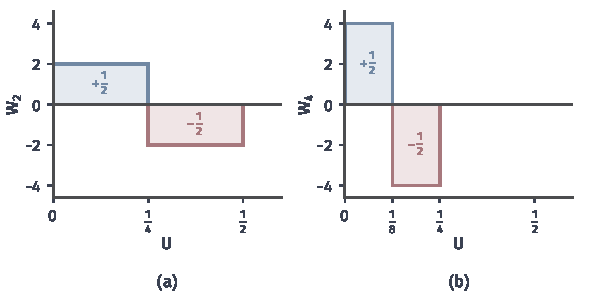
\includegraphics[width=100mm]{figures/07-probability/03-probability-limits/matplotlib/rvconv-signed-cancel/figure.pdf}
 \caption{正负抵消的变量$W_n$作为$U$的函数。浅蓝块是正的部分，面积$1/2$；浅红块是负的部分，面积$1/2$。(a)$n=2$。(b)$n=4$。期望恒为$0$，平均绝对误差恒为$1$。}
 \label{fig:rvconv-signed-cancel}
\end{BookInlineFigure}

图~\ref{fig:rvconv-signed-cancel}中正负两块面积相等，期望恰好是零，与极限$0$的期望相同；但两块的绝对面积加起来是$1$，平均绝对误差没有消失。$\{W_n\}$不一致可积，与$Y_n$同理。期望收敛只是一个数的收敛，平均绝对误差的消失才是误差本身在平均意义下的消失。

对非负变量，抵消不会发生，两者等价。

\begin{lemma}[Scheffé引理]
\label{lem:rvconv-scheffe}
设$X_n\geq0$，$X_n\xrightarrow{\mathbb{P}}X$，$\mathbb{E}[X]<\infty$，且$\mathbb{E}[X_n]\to\mathbb{E}[X]$。则$\mathbb{E}[\lvert X_n-X\rvert]\to0$。
\end{lemma}

\begin{proof}
依概率收敛的子列几乎必然收敛，所以$X\geq0$几乎必然。把绝对值拆成正部与负部，$\lvert a\rvert=a+2\max\{-a,0\}$，取$a=X_n-X$，得到
\[
 \mathbb{E}\bigl[\lvert X_n-X\rvert\bigr]=\bigl(\mathbb{E}[X_n]-\mathbb{E}[X]\bigr)+2\,\mathbb{E}\bigl[(X-X_n)^{+}\bigr] .
\]
第一项按假设趋于零。第二项中$0\leq(X-X_n)^{+}\leq X$，这里用到$X_n\geq0$；$(X-X_n)^{+}$依概率收敛到$0$，又被可积的$X$控制，由依概率收敛下的支配收敛，它的期望趋于零。
\end{proof}

这个结论称为\term{Scheffé引理}（Scheffé's lemma）。非负性让负部被极限$X$从上方压住，正部的大小又由期望之差决定，抵消无处藏身。$Y_n$也是非负的，但$\mathbb{E}[Y_n]=1$不趋于$\mathbb{E}[0]=0$，引理的条件不满足，这与它不$L^{1}$收敛一致。


\section{本章小结}
\label{sec:rvconv-summary}

本章在同一个概率空间上研究随机误差$X_n-X$怎样趋于零。三种收敛方式对应三种要求：几乎必然收敛看每条记录上的数列，允许一个零概率的例外集；依概率收敛看每一项超差事件的概率；$L^{p}$收敛看误差$p$次幂的平均。表~\ref{tab:rvconv-summary}列出它们各自控制和放过的东西。

\begin{BookInlineTable}
 \centering
 \begin{tabular}{@{}lll@{}}
  \toprule
  收敛方式 & 要求 & 不控制 \\
  \midrule
  几乎必然 & 几乎每条记录最终不再超差 & 超差的幅度 \\
  依概率 & 每项超差的概率趋于零 & 反复超差、超差的幅度 \\
  $L^{p}$ & 误差$p$次幂的期望趋于零 & 同一记录的反复超差 \\
  \bottomrule
 \end{tabular}
 \caption{三种收敛方式的要求与盲点。}
 \label{tab:rvconv-summary}
\end{BookInlineTable}

几乎必然收敛与$L^{p}$收敛都推出依概率收敛，较高阶的$L^{p}$收敛推出较低阶的。反方向的失败有两种来源。稀有大值$Y_n$、$Z_n$缺的是尾部控制：超差越来越少，但每次越来越大。移动区块$B_n$与独立示性变量$\xi_n$缺的是整列的逐样本控制：超差事件越来越小，却在每条记录上反复出现。图~\ref{fig:rvconv-implications}汇总了这些关系，以及补上缺陷后可以反向推出的结论。

\begin{BookInlineFigure}
 \centering
 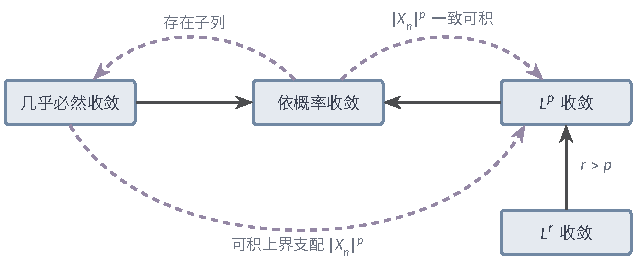
\includegraphics[width=108mm]{figures/07-probability/03-probability-limits/tikz/rvconv-implications/figure.pdf}
 \caption{同一概率空间上收敛方式之间的关系，$1\leq p<r<\infty$。深灰实线箭头总是成立；紫色虚线箭头在所标条件下成立：依概率收敛的列存在几乎必然收敛的子列，依概率收敛加上$\{\lvert X_n\rvert^{p}\}$一致可积推出$L^{p}$收敛，几乎必然收敛加上$\lvert X_n\rvert^{p}$有共同可积上界推出$L^{p}$收敛。}
 \label{fig:rvconv-implications}
\end{BookInlineFigure}

几乎必然行为由事件的重复来判断。误差最终小于$\varepsilon$，就是超差事件只发生有限次；只需对可数个阈值检查。超差概率可以求和时，Borel–Cantelli引理不需要任何独立性就保证有限次发生；概率不可求和时，只有在独立条件下才能断言无穷多次发生，没有独立性则什么都推不出。依概率收敛的列总有几乎必然收敛的子列，而依概率收敛恰好等价于“每个子列都有几乎必然收敛的进一步子列”。

期望与极限的交换由尾部控制决定。单调递增的非负列不会丢失期望，极限期望可以为无穷。不单调时，Fatou引理只给出单向的不等式，丢失的部分是逃到远处的质量。共同的可积上界阻止质量逃逸，给出支配收敛；它真正控制的是整族变量在大取值处的贡献，把这一点单独拿出来就是一致可积性。共同上界和高于一阶的一致矩界都推出一致可积，一阶矩一致有界则不够。在依概率收敛的前提下，$L^{1}$收敛与一致可积等价。平均绝对误差的消失还要和有符号期望的收敛区分开，对非负变量两者才等价。

下一章研究独立随机变量的部分和与样本平均，检验它们怎样满足本章的这些要求：有限方差给出均方误差的估计和依概率收敛，强大数律则要用到几乎必然收敛的判别工具。本章始终要求各变量定义在同一个概率空间上，误差$X_n-X$才有意义；只比较各自的分布、不要求共同实现的收敛由第~\ref{chap:weak-convergence-of-distributions}章研究。


\chapter{独立和与大数律}
\label{chap:laws-of-large-numbers}

掷一颗均匀骰子，点数的期望是$3.5$。掷$n$次后把点数平均，这个平均会不会越来越接近$3.5$？直觉说会，第~\ref{chap:random-variable-moments}章也正是用“多次重复的平均”来引出期望的。可是“接近”有两种不同的说法：对固定的$n$，平均偏离$3.5$超过$0.1$的概率很小；或者，几乎每一串实际掷出的点数，其平均最终都停在$3.5$附近。前一种只说每个时刻出错的机会，后一种说的是整条记录的最终走向。

另一个问题看起来不同。随机地给调和级数的每一项配上正负号，得到$\sum_k\varepsilon_k/k$，其中$\varepsilon_k$独立地以各$1/2$的概率取$\pm1$。不加符号时级数发散，加了随机符号以后，部分和会不会停下来？这里没有除以项数，问的是无限累计本身是否收敛。

两类问题有共同的对象：独立随机变量的部分和。平均是部分和除以$n$，级数是部分和本身。本章先计算部分和的均值与方差，并用Kolmogorov最大不等式控制部分和在一整段时间内的最大偏离；这一工具首先给出随机级数的收敛判据，再经截断推广为三系列定理。随后转向平均：弱大数律用方差或截断控制固定时刻的偏差概率，强大数律借Kronecker引理把加权级数的收敛翻译成平均的收敛。最后把频率、函数平均与样本矩写成独立同分布变量的平均，逐项核对条件。

全章使用第~\ref{chap:random-variable-convergence}章的几种收敛方式、Borel–Cantelli引理与支配收敛定理，独立性的一般含义取自第~\ref{chap:probability-spaces}章。

\section{独立部分和}
\label{sec:lln-partial-sums}

全章固定一个概率空间$(\Omega,\mathcal{F},\mathbb{P})$，在上面取一列随机变量$X_1,X_2,\dots$，并假设它们相互独立：其中任意有限个都相互独立。按第~\ref{chap:probability-spaces}章的结论，这些变量的函数，只要所用的下标组互不相交，也相互独立。例如$X_1+X_2$与$X_3X_4$独立，前$k$项的任何函数与第$k+1$项以后有限项的任何函数独立。

把前$n$项依次加起来，就得到一个随机的累计量。固定一个样本点$\omega$，$n\mapsto X_1(\omega)+\dots+X_n(\omega)$是一个普通的实数列，可以画成一条折线，每一步增加一个独立的增量。本章的所有问题都问这条折线的长期行为：它本身是否停在某处，或者除以步数以后是否停在某处。

\subsection{中心化与归一化}
\label{sec:lln-normalization}

同一列累计和可以按三种方式观察，它们回答的问题不同，先把记号定下来。

\begin{definition}[部分和、中心化部分和与样本平均]
\label{def:lln-partial-sums}
设$X_1,X_2,\dots$可积，记$\mu_k=\mathbb{E}[X_k]$。对$n\geq1$，令
\begin{equation}
 \begin{gathered}
 S_n=\sum_{k=1}^{n}X_k,\qquad \bar{X}_n=\frac{S_n}{n},\\
 \tilde{S}_n=\sum_{k=1}^{n}(X_k-\mu_k)=S_n-\mathbb{E}[S_n],
 \end{gathered}
 \label{eq:lln-partial-sums}
\end{equation}
并约定$S_0=\tilde{S}_0=0$。分别称$S_n$、$\tilde{S}_n$、$\bar{X}_n$为\term{部分和}（partial sum）、\term{中心化部分和}（centered partial sum）与\term{样本平均}（sample average）。
\end{definition}

$\mathbb{E}[S_n]=\sum_{k\leq n}\mu_k$用的是期望的线性性，下一小节再细看。部分和$S_n$收敛到有限极限，就是随机级数$\sum_kX_k$收敛，这是关于无限累计本身的问题。中心化部分和$\tilde{S}_n$去掉了各项的平均漂移，只剩随机波动；它是否收敛，问的是波动的累计能否停下来。样本平均$\bar{X}_n$把累计量按步数摊平，问的是每一步的平均贡献是否稳定。

\paragraph{同一列变量的不同答案}
取$X_k=\varepsilon_k$，其中$\varepsilon_1,\varepsilon_2,\dots$独立，各以$1/2$的概率取$+1$和$-1$。这样的$\varepsilon_k$称为随机符号，后文反复使用。这时$\mu_k=0$，三种部分和中前两种相同。$S_n$不可能收敛：相邻两项总相差$\lvert S_{n+1}-S_n\rvert=1$，对每个样本点都不是Cauchy列。平均$\bar{X}_n=S_n/n$却表现得很安稳。

图~\ref{fig:lln-three-normalizations}画出同一组五条路径的两种观察。图(a)中$S_n$在零的两侧来回游荡，偏离的典型大小与紫色虚线$\pm\sqrt{n}$同阶；图(b)中把同样的路径除以$n$，波动按$1/\sqrt{n}$收窄。下一小节会说明$\sqrt{n}$与$1/\sqrt{n}$分别是$S_n$与$\bar{X}_n$的标准差。

\begin{BookInlineFigure}
 \centering
 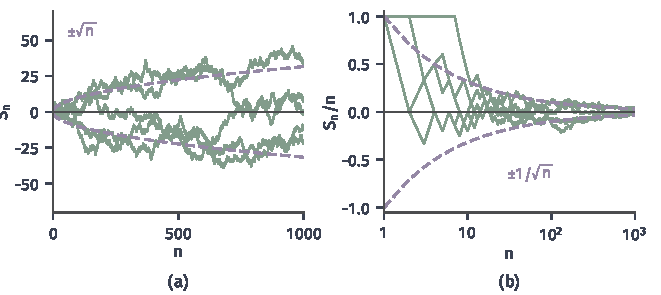
\includegraphics[width=112mm]{figures/07-probability/03-probability-limits/matplotlib/lln-three-normalizations/figure.pdf}
 \caption{随机符号的部分和与样本平均，五条路径（种子$7$）。(a)部分和$S_n$（绿线）与$\pm\sqrt{n}$（紫色虚线），横轴为线性刻度；(b)样本平均$S_n/n$（绿线）与$\pm1/\sqrt{n}$（紫色虚线），横轴为对数刻度。}
 \label{fig:lln-three-normalizations}
\end{BookInlineFigure}

反过来，给每一项加上递减的权重，累计也可能收敛。下一节将证明$\sum_k\varepsilon_k/k$几乎必然收敛，而$\sum_k\varepsilon_k/\sqrt{k}$几乎必然发散。级数问题与平均问题都由部分和出发，但所用的尺度不同，结论也就不同。

\paragraph{各项均值不同时}
当$X_k$不同分布时，各项均值$\mu_k$可以互不相同，中心化必须逐项减去自己的$\mu_k$。如果$\mu_k$的平均本身不收敛，就不存在一个共同的数可以作为$\bar{X}_n$的极限。

看一个具体的例子。令$X_k\sim\operatorname{Bern}(p_k)$相互独立，其中
\[
 p_k=\begin{cases}0.2, & 2^j\leq k<2^{j+1},\ j\ \text{为偶数},\\ 0.8, & 2^j\leq k<2^{j+1},\ j\ \text{为奇数}.\end{cases}
\]
第$j$段含$2^j$项，比前面所有段的项数之和还多一项，所以每走完一段，前$n$项均值的平均
\[
 m_n=\frac{1}{n}\sum_{k=1}^{n}p_k
\]
就被最后一段拉向它自己的取值。

具体算一下极限点。在第$J$段末尾$n=2^{J+1}-1$处，最后一段约占全部项数的$1/2$，倒数第二段约占$1/4$，依此类推。$J$为奇数时，取$0.8$的段占比约为$1/2+1/8+\dots=2/3$，于是
\[
 m_n\to0.8\cdot\tfrac23+0.2\cdot\tfrac13=0.6 ;
\]
$J$为偶数时两种取值的占比对调，$m_n\to0.4$。所以$m_n$在$0.4$与$0.6$之间往复，没有极限。

图~\ref{fig:lln-varying-means}(a)中蓝线是$m_n$，绿线是一条样本路径的$S_n/n$，后者紧跟前者摆动；图(b)画出两者之差$(S_n-\sum_{k\leq n}p_k)/n=\tilde{S}_n/n$，它趋于零。正确的问题因此是$\tilde{S}_n/n\to0$，而不是“$\bar{X}_n$趋于某个共同期望”。第~\ref{sec:lln-series-to-average}小节将证明，对这个例子$\tilde{S}_n/n$几乎必然趋于零。

\begin{BookInlineFigure}
 \centering
 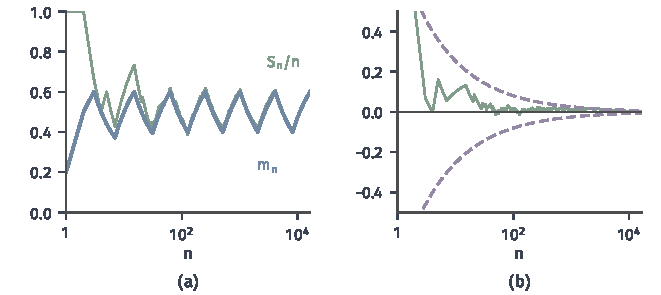
\includegraphics[width=112mm]{figures/07-probability/03-probability-limits/matplotlib/lln-varying-means/figure.pdf}
 \caption{分段取均值的独立Bernoulli变量，$p_k$在长度倍增的各段上交替取$0.2$与$0.8$，一条路径（种子$3$），横轴为对数刻度。(a)均值的平均$m_n$（蓝线）与样本平均$S_n/n$（绿线）；(b)差$(S_n-\sum_{k\leq n}p_k)/n$（绿线）与两倍标准差包络（紫色虚线）。}
 \label{fig:lln-varying-means}
\end{BookInlineFigure}

\subsection{均值与方差}
\label{sec:lln-mean-variance}

要判断累计量的走向，先看它在一个固定终点$n$处的中心和散布。中心由期望给出，不需要独立；散布由方差给出，独立性在这里第一次起作用。

\begin{theorem}[独立和的均值与方差]
\label{thm:lln-mean-variance}
设$X_1,\dots,X_n$可积，$\mu_k=\mathbb{E}[X_k]$。则
\begin{equation}
 \mathbb{E}[S_n]=\sum_{k=1}^{n}\mu_k .
 \label{eq:lln-sum-mean}
\end{equation}
若进一步$X_1,\dots,X_n$相互独立，且$\sigma_k^2=\operatorname{Var}(X_k)<\infty$，则
\begin{equation}
 \operatorname{Var}(S_n)=\mathbb{E}[\tilde{S}_n^2]=\sum_{k=1}^{n}\sigma_k^2 .
 \label{eq:lln-sum-variance}
\end{equation}
式~\eqref{eq:lln-sum-variance}只用到两两不相关，即$j\neq k$时$\operatorname{Cov}(X_j,X_k)=0$。
\end{theorem}

\begin{proof}
式~\eqref{eq:lln-sum-mean}是期望的线性性。对方差，记$D_k=X_k-\mu_k$，则$\tilde{S}_n=\sum_kD_k$。把平方展开成对角项与交叉项：
\[
 \tilde{S}_n^2=\sum_{k=1}^{n}D_k^2+\sum_{j\neq k}D_jD_k .
\]
由$\lvert D_jD_k\rvert\leq(D_j^2+D_k^2)/2$，每个交叉项都可积。$X_j$与$X_k$独立时，$D_j$与$D_k$也独立，乘积的期望等于期望的乘积，见第~\ref{chap:random-vectors}章，于是
\[
 \mathbb{E}[D_jD_k]=\mathbb{E}[D_j]\,\mathbb{E}[D_k]=0\cdot0=0 .
\]
对展开式取期望，交叉项全部消失，剩下$\sum_k\mathbb{E}[D_k^2]=\sum_k\sigma_k^2$。这一步只用了$\mathbb{E}[D_jD_k]=\operatorname{Cov}(X_j,X_k)=0$。
\end{proof}

\paragraph{波动为什么只按平方根增长}
把方差看作质量绕重心的转动惯量。独立的偏差有正有负，互相部分抵消，所以$n$项的总转动惯量只是各项之和，而不是像同向偏差那样按$n^2$增长。对比极端的相关情形：若$X_k=X_1$对所有$k$成立，则$S_n=nX_1$，方差为$n^2\sigma_1^2$。独立同分布、方差为$\sigma^2$时，式~\eqref{eq:lln-sum-variance}给出
\[
 \operatorname{Var}(S_n)=n\sigma^2,\qquad \operatorname{Var}(\bar{X}_n)=\frac{\sigma^2}{n} .
\]
部分和的标准差是$\sqrt{n}\,\sigma$，样本平均的标准差是$\sigma/\sqrt{n}$，这正是图~\ref{fig:lln-three-normalizations}中两条包络的来历。

\paragraph{固定终点的偏差}
对中心化部分和用第~\ref{chap:tail-probabilities}章的Chebyshev不等式，就得到终点处偏差的概率上界：对每个$a>0$，
\begin{equation}
 \mathbb{P}\bigl(\lvert\tilde{S}_n\rvert\geq a\bigr)\leq\frac{1}{a^2}\sum_{k=1}^{n}\sigma_k^2 .
 \label{eq:lln-endpoint-chebyshev}
\end{equation}

用骰子检验一下。掷$n=100$次均匀骰子，单次点数的方差为$35/12$，所以
\[
 \operatorname{Var}(S_{100})=100\cdot\frac{35}{12}=\frac{875}{3}\approx291.7 .
\]
取$a=30$，式~\eqref{eq:lln-endpoint-chebyshev}给出
\[
 \mathbb{P}\bigl(\lvert S_{100}-350\rvert\geq30\bigr)\leq\frac{291.7}{900}\approx0.324 .
\]
用$200000$条模拟路径（种子$12$）估计，左边约为$0.085$。界偏大，但它对任何方差为$35/12$的独立同分布序列都成立。

\paragraph{终点控制不住整段路径}
式~\eqref{eq:lln-endpoint-chebyshev}只管时刻$n$。部分和可以先越过$\pm a$，再回到区间内部。图~\ref{fig:lln-endpoint-vs-path}画出$30$条骰子路径（种子$11$），其中$4$条在$k\leq100$的某一步越过了$\pm30$，有$3$条到$k=100$时又回到了带内。模拟估计全程越过的概率约为$0.147$，比终点越过的$0.085$大不少。

\begin{BookInlineFigure}
 \centering
 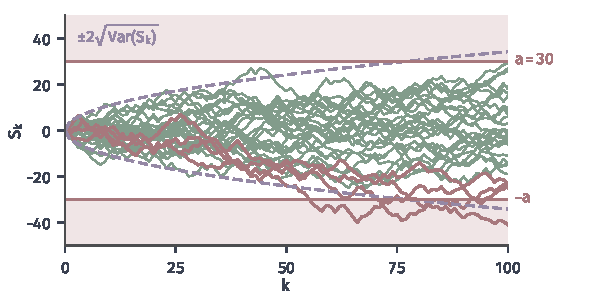
\includegraphics[width=100mm]{figures/07-probability/03-probability-limits/matplotlib/lln-endpoint-vs-path/figure.pdf}
 \caption{中心化骰子部分和$S_k=\sum_{i\leq k}(D_i-3.5)$的$30$条路径（种子$11$），$k\leq100$。红色水平线为阈值$\pm30$，浅红区域为越界区域；红线是在某一步越过阈值的路径，绿线是始终未越过的路径；紫色虚线为$\pm2\sqrt{\operatorname{Var}(S_k)}$。}
 \label{fig:lln-endpoint-vs-path}
\end{BookInlineFigure}

一个朴素的补救是对每个$k\leq n$分别用Chebyshev不等式再相加。独立同分布、方差为$\sigma^2$时，
\[
 \mathbb{P}\Bigl(\max_{k\leq n}\lvert\tilde{S}_k\rvert\geq a\Bigr)\leq\sum_{k=1}^{n}\frac{\operatorname{Var}(S_k)}{a^2}=\frac{\sigma^2}{a^2}\cdot\frac{n(n+1)}{2} .
\]
骰子例子中右边约为$16.4$，远大于$1$，毫无用处。各个时刻的越界事件高度重叠，相加把同一块概率计算了许多次。下一小节说明，对独立中心化的和，整段路径的最大偏离与终点偏差满足同一个上界。

\subsection{Kolmogorov最大不等式}
\label{sec:lln-maximal-inequality}

先猜一下最大偏离应当满足怎样的界。一条路径若在某一步$k$首次越过$a$，此后的增量既独立于过去，平均又为零，没有系统地把路径拉回来的倾向。所以终点平方的期望至少还保留着越界时的$S_k^2\geq a^2$。这就是说，越过阈值的路径不会因为“回头”而在终点的方差中消失。

\begin{theorem}[Kolmogorov最大不等式]
\label{thm:lln-kolmogorov-maximal}
设$X_1,\dots,X_n$相互独立，$\mathbb{E}[X_k]=0$，$\mathbb{E}[X_k^2]<\infty$。则对每个$a>0$，
\begin{equation}
 \mathbb{P}\Bigl(\max_{1\leq k\leq n}\lvert S_k\rvert\geq a\Bigr)\leq\frac{\operatorname{Var}(S_n)}{a^2}=\frac{1}{a^2}\sum_{k=1}^{n}\mathbb{E}[X_k^2] .
 \label{eq:lln-kolmogorov-maximal}
\end{equation}
\end{theorem}

这个不等式称为\term{Kolmogorov最大不等式}（Kolmogorov's maximal inequality）。它的右边与终点的Chebyshev界~\eqref{eq:lln-endpoint-chebyshev}完全相同，左边却换成了整段路径的最大值。

\begin{proof}
按首次越过阈值的时刻把事件拆开。对$k=1,\dots,n$，令
\[
 A_k=\bigl\{\lvert S_k\rvert\geq a,\ \lvert S_j\rvert<a\ \text{对所有}\ j<k\bigr\} .
\]
$A_k$表示“在第$k$步首次越过”。这些事件两两不交，它们的并恰为$A=\{\max_{k\leq n}\lvert S_k\rvert\geq a\}$。

由于$S_n^2\geq0$，且$A_1,\dots,A_n$不交，
\[
 \mathbb{E}[S_n^2]\geq\mathbb{E}[S_n^2\mathbf{1}_{A}]=\sum_{k=1}^{n}\mathbb{E}[S_n^2\mathbf{1}_{A_k}] .
\]
固定$k$，把终点写成首次越过时的位置加上之后的增量，$S_n=S_k+(S_n-S_k)$。展开平方并丢掉非负项$(S_n-S_k)^2$，得到
\[
 S_n^2\geq S_k^2+2S_k(S_n-S_k) .
\]

关键是交叉项的期望为零。$S_k\mathbf{1}_{A_k}$只依赖$X_1,\dots,X_k$，$S_n-S_k=X_{k+1}+\dots+X_n$只依赖后面的变量，两者独立，并且都平方可积。于是
\[
 \mathbb{E}\bigl[S_k\mathbf{1}_{A_k}(S_n-S_k)\bigr]=\mathbb{E}[S_k\mathbf{1}_{A_k}]\,\mathbb{E}[S_n-S_k]=0 .
\]

把上面的不等式乘以$\mathbf{1}_{A_k}$再取期望，交叉项消失。再利用$A_k$上$S_k^2\geq a^2$，得到
\[
 \mathbb{E}[S_n^2\mathbf{1}_{A_k}]\geq\mathbb{E}[S_k^2\mathbf{1}_{A_k}]\geq a^2\,\mathbb{P}(A_k) .
\]
对$k$求和，并利用$A_1,\dots,A_n$不交，得到
\[
 \mathbb{E}[S_n^2]\geq a^2\sum_{k=1}^{n}\mathbb{P}(A_k)=a^2\,\mathbb{P}(A) .
\]
最后由式~\eqref{eq:lln-sum-variance}，左边等于$\operatorname{Var}(S_n)=\sum_k\mathbb{E}[X_k^2]$，两边除以$a^2$即得。
\end{proof}

图~\ref{fig:lln-first-passage}把证明中的分解画了出来。首次越过时刻$k$之前的信息决定了$A_k$与$S_k$，之后的增量与它们独立且平均为零。路径越界后可能回到带内，但这种回头只是随机的，平均来说不抵消越界时已有的$S_k^2$。

\begin{BookInlineFigure}
 \centering
 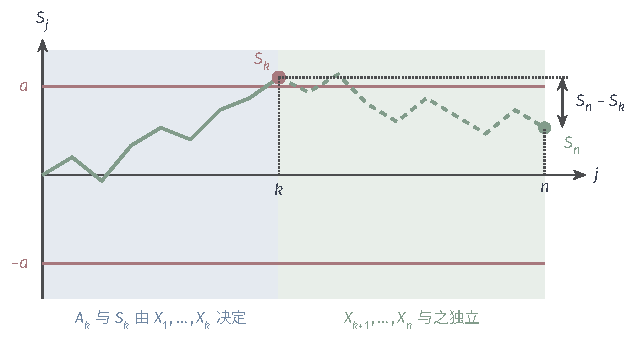
\includegraphics[width=107mm]{figures/07-probability/03-probability-limits/tikz/lln-first-passage/figure.pdf}
 \caption{Kolmogorov最大不等式的首次越过分解（示意）。绿色折线为部分和路径，在第$k$步首次达到$\lvert S_k\rvert\geq a$（红点）；浅蓝区域内的信息决定事件$A_k$，浅绿区域内的增量$X_{k+1},\dots,X_n$与之独立；终点$S_n=S_k+(S_n-S_k)$可以回到阈值以内。}
 \label{fig:lln-first-passage}
\end{BookInlineFigure}

\paragraph{一个能逐条数清的例子}
取四个随机符号，$S_k=\varepsilon_1+\dots+\varepsilon_k$，共有$2^4=16$条等可能的路径，阈值取$a=3$。图~\ref{fig:lln-rademacher-lattice}在每个节点标出经过它的路径条数。要在四步内达到$\lvert S_k\rvert\geq3$，必须前三步同号，到达$(3,\pm3)$；从那里第四步可上可下，所以共有$2\times2=4$条路径越界。终点满足$\lvert S_4\rvert\geq3$的只有终点为$\pm4$的$2$条。

\begin{BookInlineFigure}
 \centering
 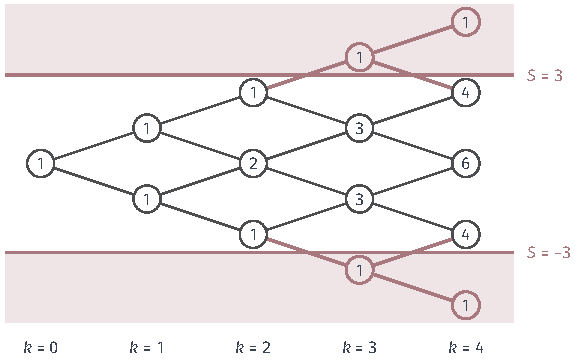
\includegraphics[width=98mm]{figures/07-probability/03-probability-limits/tikz/lln-rademacher-lattice/figure.pdf}
 \caption{四个随机符号的全部$16$条路径。节点中的数字是经过该节点的路径条数；红色水平线为$S=\pm3$，红色边与红框节点标出在某一步达到$\lvert S_k\rvert\geq3$的$4$条路径，其中$2$条在第四步回到$\pm2$。}
 \label{fig:lln-rademacher-lattice}
\end{BookInlineFigure}

于是三个量分别是
\[
 \begin{gathered}
 \mathbb{P}\Bigl(\max_{k\leq4}\lvert S_k\rvert\geq3\Bigr)=\frac{4}{16}=0.25,\qquad
 \mathbb{P}(\lvert S_4\rvert\geq3)=\frac{2}{16}=0.125,\\
 \frac{\operatorname{Var}(S_4)}{3^2}=\frac49\approx0.444 .
 \end{gathered}
\]
最大偏离的概率是终点概率的两倍，仍在Kolmogorov界之下。若取$a=2$，同样计数得到$0.75$、$0.625$与界$1$。

\paragraph{较长的路径}
图~\ref{fig:lln-maximal-compare}对$n=100$个随机符号精确计算两种概率：终点概率由二项分布求和，全程最大值越界的概率由逐步递推（越界即吸收）求得。$a=20$时终点概率为$0.057$，全程概率为$0.092$，Kolmogorov界为$0.25$，逐点相加的界却是$12.6$。Kolmogorov界与真实值的差距来自它只用了方差；真正的尾部还要轻得多，那是第~\ref{chap:central-limit-theorem}章的内容。

\begin{BookInlineFigure}
 \centering
 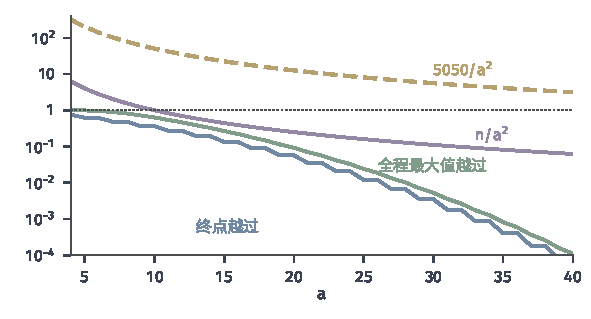
\includegraphics[width=100mm]{figures/07-probability/03-probability-limits/matplotlib/lln-maximal-compare/figure.pdf}
 \caption{$n=100$个随机符号，越界概率随阈值$a$的变化，纵轴为对数刻度。蓝线为终点概率$\mathbb{P}(\lvert S_n\rvert\geq a)$，绿线为全程最大值概率$\mathbb{P}(\max_{k\leq n}\lvert S_k\rvert\geq a)$，二者均为精确值；紫线为Kolmogorov界$n/a^2$，黄色虚线为逐点相加的界$\sum_{k\leq n}k/a^2=5050/a^2$，点线标出概率$1$。}
 \label{fig:lln-maximal-compare}
\end{BookInlineFigure}

\paragraph{条件各起什么作用}
中心化不可省略。若$X_k\equiv1$，方差为零，式~\eqref{eq:lln-kolmogorov-maximal}右边为$0$，而$\max_{k\leq n}\lvert S_k\rvert=n$。证明中用到的是$\mathbb{E}[S_n-S_k]=0$：有漂移时，越界之后的路径会被系统地推向一侧，平方的期望不再只由方差决定。

独立性也不可省略，它保证了交叉项的期望为零。取$X_1=\varepsilon_1$，$X_2=-\varepsilon_1$，两项都中心化且方差为$1$，但$S_2=0$，右边为$0$；左边在$a=1$时却等于$\mathbb{P}(\lvert S_1\rvert\geq1)=1$。这里第二步完全由第一步决定，越界后被确定地拉了回来。

这个不等式是本章的主要工具。下一节用它控制随机级数的尾段，第~\ref{sec:lln-strong-law}节再经由级数得到强大数律。


\section{独立随机级数}
\label{sec:lln-random-series}

回到章首的随机调和级数$\sum_k\varepsilon_k/k$。确定的调和级数$\sum_k1/k$发散，是因为每一项都向同一方向推；随机符号让各项方向随机，推力互相抵消。抵消到什么程度，部分和才会停下来？

一般地，设$X_1,X_2,\dots$独立，问部分和$S_n=\sum_{k\leq n}X_k$是否几乎必然收敛到一个有限的极限$S$。这样的$\sum_kX_k$称为\term{随机级数}（random series）。对每个样本点$\omega$，这是一个普通的数项级数，收敛与否由Cauchy准则判断：
\[
 S_n(\omega)\ \text{收敛}\iff \sup_{j,k>m}\lvert S_j(\omega)-S_k(\omega)\rvert\to0\quad(m\to\infty) .
\]
上确界只需在可数个下标上取，所以“级数收敛”是一个事件。我们要证明的是这个事件的概率为一。

图~\ref{fig:lln-random-harmonic}用同一组随机符号画出两个级数的部分和。图(a)中$\sum_k\varepsilon_k/k$的六条路径在$n=100$以后几乎不再移动，各自停在不同的高度；图(b)中$\sum_k\varepsilon_k/\sqrt{k}$的路径一直在游荡，摆幅与紫色包络$\pm2\sqrt{H_n}$同步扩大，其中$H_n=\sum_{k\leq n}1/k$。两者的区别正在于各项方差之和：前者$\sum_k1/k^2<\infty$，后者$\sum_k1/k=\infty$。

\begin{BookInlineFigure}
 \centering
 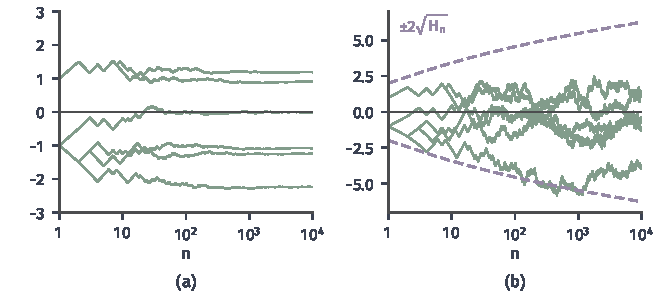
\includegraphics[width=112mm]{figures/07-probability/03-probability-limits/matplotlib/lln-random-harmonic/figure.pdf}
 \caption{同一组随机符号（种子$5$）下两个随机级数的部分和，六条路径，横轴为对数刻度。(a)$\sum_{k\leq n}\varepsilon_k/k$；(b)$\sum_{k\leq n}\varepsilon_k/\sqrt{k}$，紫色虚线为$\pm2\sqrt{H_n}$，$H_n=\sum_{k\leq n}1/k$。}
 \label{fig:lln-random-harmonic}
\end{BookInlineFigure}

\subsection{方差可和的情形}
\label{sec:lln-variance-series}

收敛需要控制部分和的整个尾段，而不仅是某一个时刻的增量。Kolmogorov最大不等式恰好控制一整段路径的最大偏离，把它用在从第$m+1$项开始的尾段上，偏离的概率由尾段方差之和决定。方差可和时，这个尾和趋于零。

\begin{theorem}[方差可和的随机级数]
\label{thm:lln-variance-series}
设$X_1,X_2,\dots$相互独立，$\mathbb{E}[X_k]=0$，并且
\begin{equation}
 \sum_{k=1}^{\infty}\mathbb{E}[X_k^2]<\infty .
 \label{eq:lln-variance-summable}
\end{equation}
则$\sum_kX_k$几乎必然收敛到一个有限的随机变量$S$。此外$S_n\xrightarrow{L^{2}}S$，并且$\mathbb{E}[S]=0$，$\mathbb{E}[S^2]=\sum_k\mathbb{E}[X_k^2]$。
\end{theorem}

\begin{proof}
记$\sigma_k^2=\mathbb{E}[X_k^2]$。对$m\geq0$，令
\[
 V_m=\sup_{j,k>m}\lvert S_j-S_k\rvert,\qquad W_m=\sup_{k>m}\lvert S_k-S_m\rvert ,
\]
二者取值于$[0,\infty]$。$V_m$随$m$不增，所以极限$V=\lim_mV_m$存在，并且部分和是Cauchy列当且仅当$V=0$。对$j,k>m$用三角不等式，
\[
 \lvert S_j-S_k\rvert\leq\lvert S_j-S_m\rvert+\lvert S_k-S_m\rvert\leq2W_m ,
\]
所以$V_m\leq2W_m$。

先估计$W_m$。固定$m$与$\varepsilon>0$，对$N>m$考虑事件
\[
 E_N=\Bigl\{\max_{m<k\leq N}\lvert S_k-S_m\rvert>\varepsilon\Bigr\} .
\]
$E_N$随$N$增大而增大，并上升到$\{W_m>\varepsilon\}$。尾段$S_k-S_m=X_{m+1}+\dots+X_k$是独立中心化变量的部分和，对它用定理~\ref{thm:lln-kolmogorov-maximal}，得到
\[
 \mathbb{P}(E_N)\leq\frac{1}{\varepsilon^2}\sum_{k=m+1}^{N}\sigma_k^2\leq\frac{1}{\varepsilon^2}\sum_{k>m}\sigma_k^2 .
\]
令$N\to\infty$，由概率的连续性，
\begin{equation}
 \mathbb{P}(W_m>\varepsilon)\leq\frac{1}{\varepsilon^2}\sum_{k>m}\sigma_k^2 .
 \label{eq:lln-tail-oscillation}
\end{equation}

再回到$V$。由于$V\leq V_m\leq2W_m$，对每个$m$，
\[
 \mathbb{P}(V>2\varepsilon)\leq\mathbb{P}(W_m>\varepsilon)\leq\frac{1}{\varepsilon^2}\sum_{k>m}\sigma_k^2 .
\]
左边与$m$无关，右边是收敛级数~\eqref{eq:lln-variance-summable}的尾和，令$m\to\infty$趋于零。所以对每个$\varepsilon>0$都有$\mathbb{P}(V>2\varepsilon)=0$。取$\varepsilon=1/j$并对$j$取可数并，得到$\mathbb{P}(V>0)=0$。于是几乎必然地，$S_n$是Cauchy列，收敛到有限极限$S$。

最后看$L^2$收敛。由式~\eqref{eq:lln-sum-variance}，$N>m$时
\[
 \mathbb{E}\bigl[(S_N-S_m)^2\bigr]=\sum_{k=m+1}^{N}\sigma_k^2\leq\sum_{k>m}\sigma_k^2\to0 .
\]
所以$S_n$在$L^2$中是Cauchy列，收敛到某个$S'\in L^2$。由第~\ref{chap:random-variable-convergence}章，$L^2$收敛的序列有几乎必然收敛的子列，其极限只能是$S$，故$S'=S$几乎必然成立。$L^2$收敛蕴含一阶矩与二阶矩收敛，于是
\[
 \mathbb{E}[S]=\lim_{n\to\infty}\mathbb{E}[S_n]=0,\qquad \mathbb{E}[S^2]=\lim_{n\to\infty}\mathbb{E}[S_n^2]=\sum_k\sigma_k^2 .
\]
\end{proof}

证明的结构值得记住：几乎必然收敛归结为“尾段的最大振荡依概率趋于零”，而最大振荡正是Kolmogorov不等式所控制的量。只控制单个增量$S_N-S_m$的方差，只能得到$L^2$收敛，不足以说明每条路径都停下来。

\paragraph{随机调和级数}
对$X_k=\varepsilon_k/k$，各项均值为零，方差可和：
\[
 \mathbb{E}[X_k]=0,\qquad \sum_{k=1}^{\infty}\mathbb{E}[X_k^2]=\sum_{k=1}^{\infty}\frac{1}{k^2}=\frac{\pi^2}{6} .
\]
定理~\ref{thm:lln-variance-series}给出$\sum_k\varepsilon_k/k$几乎必然收敛，极限$S$的均值为$0$，方差为$\pi^2/6\approx1.645$。尾和满足$\sum_{k>m}1/k^2<1/m$，取$\varepsilon=1/4$与$m=100$，式~\eqref{eq:lln-tail-oscillation}给出
\[
 \mathbb{P}\Bigl(\sup_{k>100}\lvert S_k-S_{100}\rvert>\tfrac14\Bigr)\leq16\sum_{k>100}\frac{1}{k^2}\approx16\times0.00995\approx0.159 .
\]

图~\ref{fig:lln-harmonic-limit}(b)把这个界与模拟频率放在一起比较（$4000$条路径，种子$8$，上确界在$k\leq20000$内计算）。$m=100$时模拟频率约为$0.028$。两条曲线都随$m$按$1/m$的阶下降，界比真实值宽松，但单凭方差就保证了尾段的振荡越来越罕见。

\begin{BookInlineFigure}
 \centering
 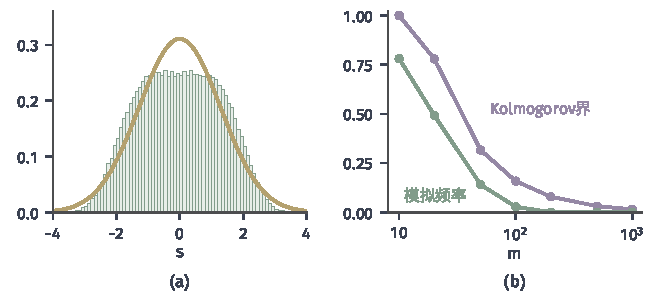
\includegraphics[width=112mm]{figures/07-probability/03-probability-limits/matplotlib/lln-harmonic-limit/figure.pdf}
 \caption{随机调和级数$\sum_k\varepsilon_k/k$的极限与尾段振荡。(a)$S_{1000}$的直方图（浅绿，$200000$个样本，种子$2$）与方差相同的高斯密度$\mathcal{N}(0,\pi^2/6)$（黄线）；(b)尾段最大振荡$\max_{m<k\leq20000}\lvert S_k-S_m\rvert\geq1/4$的模拟频率（绿线，$4000$条路径，种子$8$）与Kolmogorov界$16\sum_{m<k\leq20000}1/k^2$（紫线），横轴为$m$的对数刻度。}
 \label{fig:lln-harmonic-limit}
\end{BookInlineFigure}

极限$S$是一个真正的随机变量，它的分布由全部项共同决定。图~\ref{fig:lln-harmonic-limit}(a)用$S_{1000}$代替$S$，二者之差的方差$\sum_{k>1000}1/k^2$小于$10^{-3}$。直方图顶部平坦，与同方差的高斯密度明显不同。用独立性展开四次方可以核对这一点：对$S_n=\sum_{k\leq n}a_k\varepsilon_k$，奇次项的期望为零，只剩每个下标出现偶数次的项，
\[
 \mathbb{E}[S_n^4]=\sum_{k}a_k^4+3\sum_{j\neq k}a_j^2a_k^2=3\Bigl(\sum_ka_k^2\Bigr)^2-2\sum_ka_k^4 .
\]
取$a_k=1/k$并令$n\to\infty$，用$\sum_k1/k^4=\pi^4/90$，得到
\[
 \frac{\mathbb{E}[S^4]}{(\mathbb{E}[S^2])^2}-3=-\frac{2\pi^4/90}{(\pi^2/6)^2}=-0.8 ,
\]
而高斯分布的这个值为$0$。模拟值约为$-0.81$。

\paragraph{中心化不可省略}
定理要求各项均值为零。若$X_k=1/k$是确定的常数，方差全为零，条件~\eqref{eq:lln-variance-summable}成立，级数却发散。一般地，若$\sum_k\operatorname{Var}(X_k)<\infty$，对$X_k-\mu_k$用定理~\ref{thm:lln-variance-series}，得到$\sum_k(X_k-\mu_k)$几乎必然收敛。两个级数之差是数项级数$\sum_k\mu_k$，所以
\[
 \sum_kX_k\ \text{几乎必然收敛}\iff\sum_k\mu_k\ \text{收敛} ,
\]
并且$\sum_k\mu_k$发散时$\sum_kX_k$几乎必然发散。例如取$X_k=\xi_k/k$，$\xi_k\sim\operatorname{Bern}(1/2)$独立，方差$1/(4k^2)$可和，但均值$1/(2k)$的级数发散，于是$\sum_kX_k=+\infty$几乎必然成立。方差控制随机波动，均值控制系统漂移，两件事要分别检查。

\subsection{截断与大项控制}
\label{sec:lln-truncation}

方差可和是充分条件，但不是必要条件。各项可能偶尔取极大的值，使方差甚至均值都很大或无穷，而这些大值只出现有限次，对级数是否收敛没有影响。

\paragraph{一个方差与均值都失效的例子}
令$X_1=\varepsilon_1$。对$k\geq2$，取与$\varepsilon_k$独立的事件$B_k$，$\mathbb{P}(B_k)=1/k^2$，各$B_k$与各$\varepsilon_k$全体相互独立，定义
\[
 X_k=\begin{cases}k, & B_k\ \text{发生},\\ \varepsilon_k/k, & B_k\ \text{不发生}.\end{cases}
\]
大值$k$出现的机会很小，但幅度很大。逐项计算，$k\geq2$时
\[
 \mathbb{E}[X_k]=k\cdot\frac{1}{k^2}=\frac1k,\qquad
 \operatorname{Var}(X_k)=1+\frac{1}{k^2}-\frac{1}{k^4}-\frac{1}{k^2}=1-\frac{1}{k^4} .
\]
这里用了$\mathbb{E}[X_k^2]=k^2/k^2+(1-1/k^2)/k^2$。方差之和与均值之和都发散，上一小节的判据完全用不上。

然而大项出现的概率可和：
\[
 \sum_{k\geq2}\mathbb{P}(B_k)=\frac{\pi^2}{6}-1\approx0.645<\infty .
\]
由第~\ref{chap:random-variable-convergence}章的Borel–Cantelli引理，几乎必然只有有限个$B_k$发生。对这样的样本点，从某一项起$X_k=\varepsilon_k/k$，而$\sum_k\varepsilon_k/k$几乎必然收敛，改动有限项不影响收敛。所以$\sum_kX_k$几乎必然收敛。

图~\ref{fig:lln-big-terms}画出六条路径（种子$4$）。其中三条各出现一次大项（红点，分别在$k=2,10,2$处），路径随之跳起，此后与其余路径一样停住。黄色虚线是各项期望的累计$\sum_{k\leq n}\mathbb{E}[X_k]$，按$\ln n$无限增长：期望被极少发生的大值撑大，它描述的不是典型路径。

\begin{BookInlineFigure}
 \centering
 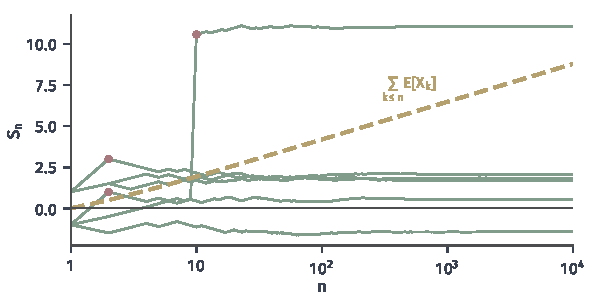
\includegraphics[width=100mm]{figures/07-probability/03-probability-limits/matplotlib/lln-big-terms/figure.pdf}
 \caption{含罕见大项的随机级数，六条路径（种子$4$），横轴为对数刻度。绿线为部分和$S_n$，红点标出大项$X_k=k$出现的位置；黄色虚线为期望的累计$\sum_{k\leq n}\mathbb{E}[X_k]=\sum_{2\leq k\leq n}1/k$。}
 \label{fig:lln-big-terms}
\end{BookInlineFigure}

\paragraph{一般的截断}
这个例子的做法可以一般化：先把大值切掉，再对剩下的有界部分分别处理均值与波动。固定$c>0$，令
\begin{equation}
 Y_k=X_k\mathbf{1}_{\{\lvert X_k\rvert\leq c\}} .
 \label{eq:lln-truncation}
\end{equation}
称$Y_k$为$X_k$在水平$c$处的\term{截断}（truncation）。每一项因此拆成三部分：
\[
 X_k=\bigl(X_k-Y_k\bigr)+\mathbb{E}[Y_k]+\bigl(Y_k-\mathbb{E}[Y_k]\bigr) .
\]
第一部分只在$\lvert X_k\rvert>c$时非零，是大项；第二部分是截断后的均值，一个普通的数；第三部分是有界的中心化波动。

三部分各需要一种控制，图~\ref{fig:lln-truncation-split}画出这种分工。

\begin{BookInlineFigure}
 \centering
 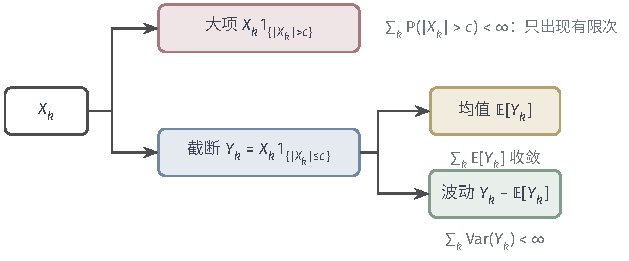
\includegraphics[width=106mm]{figures/07-probability/03-probability-limits/tikz/lln-truncation-split/figure.pdf}
 \caption{在固定水平$c$截断后的三部分及各自的控制条件。浅红框为大项，由超阈值概率之和控制；浅黄框为截断均值，由数项级数控制；浅绿框为中心化波动，由截断方差之和控制。}
 \label{fig:lln-truncation-split}
\end{BookInlineFigure}

\begin{enumerate}
 \item \emph{大项只出现有限次。}若$\sum_k\mathbb{P}(\lvert X_k\rvert>c)<\infty$，由Borel–Cantelli引理，几乎必然存在$N(\omega)$，使$k>N(\omega)$时$X_k(\omega)=Y_k(\omega)$。于是$n>N(\omega)$时$S_n(\omega)-\sum_{k\leq n}Y_k(\omega)$是一个不再变化的有限数，$\sum_kX_k$与$\sum_kY_k$同时收敛或同时发散。这一步不需要独立性，也不要求$X_k$有任何矩。
 \item \emph{截断均值的级数收敛。}$\lvert Y_k\rvert\leq c$，所以$\mathbb{E}[Y_k]$总存在。$\sum_k\mathbb{E}[Y_k]$是一个数项级数，它收敛与否与随机性无关，只能直接检查。
 \item \emph{截断波动的方差可和。}$Y_k-\mathbb{E}[Y_k]$是独立变量$X_k$的函数，彼此独立，均值为零，绝对值不超过$2c$。若$\sum_k\operatorname{Var}(Y_k)<\infty$，由定理~\ref{thm:lln-variance-series}，$\sum_k(Y_k-\mathbb{E}[Y_k])$几乎必然收敛。
\end{enumerate}

三种控制各管一件事。第一种处理方差无法描述的重尾大值；第二种处理系统性漂移；第三种处理有界的随机波动。截断水平$c$固定不变，有界性使第三步可以只用方差。回到上面的例子，取$c=1$：$k\geq2$时$\lvert X_k\rvert>1$恰好是$B_k$发生，$Y_k=\varepsilon_k\mathbf{1}_{B_k^{\mathrm{c}}}/k$，均值为$0$，方差$(1-1/k^2)/k^2$可和，三项都满足。

\subsection{三系列定理}
\label{sec:lln-three-series}

把上一小节的三种控制合在一起，就得到一个随机级数几乎必然收敛的充分条件。Kolmogorov证明了这三个条件也是必要的。

\begin{theorem}[三系列定理]
\label{thm:lln-three-series}
设$X_1,X_2,\dots$相互独立，$c>0$，$Y_k=X_k\mathbf{1}_{\{\lvert X_k\rvert\leq c\}}$。则$\sum_kX_k$几乎必然收敛，当且仅当下面三个级数都收敛：
\begin{equation}
 \sum_{k}\mathbb{P}(\lvert X_k\rvert>c),\qquad
 \sum_{k}\mathbb{E}[Y_k],\qquad
 \sum_{k}\operatorname{Var}(Y_k) .
 \label{eq:lln-three-series}
\end{equation}
\end{theorem}

这一结论称为\term{三系列定理}（three-series theorem）。注意第二个级数只要求收敛，不要求绝对收敛。例如确定的$X_k=(-1)^k/k$，取$c=1$时$Y_k=X_k$，第一、三个级数为零，第二个是条件收敛的交错级数，$\sum_kX_k$确实收敛。

\begin{proof}[充分性的证明]
设三个级数都收敛。由第三个级数与定理~\ref{thm:lln-variance-series}，$\sum_k(Y_k-\mathbb{E}[Y_k])$几乎必然收敛；加上收敛的数项级数$\sum_k\mathbb{E}[Y_k]$，$\sum_kY_k$几乎必然收敛。由第一个级数与Borel–Cantelli引理，几乎必然只有有限个$k$使$X_k\neq Y_k$，所以$\sum_kX_k$与$\sum_kY_k$同时收敛。两个几乎必然事件的交仍是几乎必然事件，结论成立。
\end{proof}

必要性中，第一个级数的必要性可以直接证明。若$\sum_kX_k$几乎必然收敛，则$X_k\to0$几乎必然，所以$\lvert X_k\rvert>c$几乎必然只发生有限次。事件$\{\lvert X_k\rvert>c\}$相互独立；如果$\sum_k\mathbb{P}(\lvert X_k\rvert>c)=\infty$，Borel–Cantelli引理的第二部分会给出它们几乎必然发生无穷多次，矛盾。

另两个级数的必要性需要更细的估计，篇幅较长，读者可查阅~\scite{math-kallenberg2021probability}。其机制是：若截断方差之和发散，有界独立波动的累计会像标准差$\sqrt{\sum_{k\leq n}\operatorname{Var}(Y_k)}$那样不断扩大，不可能停在一处，这与图~\ref{fig:lln-random-harmonic}(b)的情形相同；方差可和而均值级数发散时，前面已经说明级数几乎必然发散。同一参考书还说明，独立随机级数收敛的概率只能是$0$或$1$，所以三个级数中只要有一个发散，$\sum_kX_k$就几乎必然发散。

\paragraph{截断水平的选择}
定理对每个固定的$c>0$都成立。由必要性，若三个级数对某个$c$都收敛，则级数收敛，从而它们对所有$c>0$都收敛。实际使用时取最方便的$c$即可。

\paragraph{随机符号级数}
设$(a_k)$是有界实数列，考虑$\sum_ka_k\varepsilon_k$。取$c>\sup_k\lvert a_k\rvert$，截断不改变任何一项：第一个级数为零，$\mathbb{E}[Y_k]=0$，$\operatorname{Var}(Y_k)=a_k^2$。由三系列定理，
\begin{equation}
 \sum_ka_k\varepsilon_k\ \text{几乎必然收敛}\iff\sum_ka_k^2<\infty .
 \label{eq:lln-random-signs}
\end{equation}
取$a_k=k^{-p}$，随机符号的$p$级数几乎必然收敛当且仅当$p>1/2$。这是“抵消到什么程度”的确切答案：确定的$p$级数需要$p>1$，随机符号使门槛降到$p>1/2$，因为抵消后累计量按平方和的平方根增长。$p=1/2$正是图~\ref{fig:lln-random-harmonic}(b)的情形，那里的发散用到了这里引用的必要性部分。

后面的强大数律只用到方差可和的情形，即定理~\ref{thm:lln-variance-series}。三系列定理的作用是说明这个工具在独立级数问题中已经足够：截断之后，收敛与否就由方差和均值决定。


\section{弱大数律}
\label{sec:lln-weak-law}

现在把部分和除以$n$。设$X_1,X_2,\dots$独立同分布，共同的均值为$\mu$。在一个固定的样本量$n$下，样本平均$\bar{X}_n$偏离$\mu$超过给定精度的机会有多大，它是否随$n$增大而趋于零？用第~\ref{chap:random-variable-convergence}章的语言，问题是$\bar{X}_n$是否依概率收敛到$\mu$。

\begin{definition}[弱大数律]
\label{def:lln-weak-law}
设随机变量列$X_1,X_2,\dots$各项可积且有共同的均值$\mu$。若$\bar{X}_n\xrightarrow{\mathbb{P}}\mu$，即对每个$\varepsilon>0$，
\begin{equation}
 \lim_{n\to\infty}\mathbb{P}\bigl(\lvert\bar{X}_n-\mu\rvert\geq\varepsilon\bigr)=0 ,
 \label{eq:lln-weak-law}
\end{equation}
则称这列变量满足\term{弱大数律}（weak law of large numbers）。
\end{definition}

“平均把波动抹平”是这里的直观：每个观测的偏差有正有负，平均以后互相抵消，剩余的偏差随$n$缩小。两种情形用到的抹平机制不同。有限方差时，方差按$1/n$缩小，一步即得；只有一阶矩时，偶尔出现的大值不能用方差衡量，需要先截断。

\subsection{有限方差情形}
\label{sec:lln-wlln-variance}

方差有限时，式~\eqref{eq:lln-sum-variance}已经给出$\operatorname{Var}(\bar{X}_n)$，再用Chebyshev不等式就够了。下面的陈述把独立同分布放宽到实际用到的条件。

\begin{theorem}[有限方差的弱大数律]
\label{thm:lln-wlln-variance}
设$X_1,\dots,X_n$两两不相关，有共同的均值$\mu$，且$\operatorname{Var}(X_k)\leq\sigma^2<\infty$。则对每个$\varepsilon>0$，
\begin{equation}
 \mathbb{E}\bigl[(\bar{X}_n-\mu)^2\bigr]\leq\frac{\sigma^2}{n},\qquad
 \mathbb{P}\bigl(\lvert\bar{X}_n-\mu\rvert\geq\varepsilon\bigr)\leq\frac{\sigma^2}{n\varepsilon^2} .
 \label{eq:lln-wlln-chebyshev}
\end{equation}
特别地，独立同分布且方差有限的序列满足弱大数律，并且$\bar{X}_n\xrightarrow{L^{2}}\mu$。
\end{theorem}

\begin{proof}
$\mathbb{E}[\bar{X}_n]=\mu$。由式~\eqref{eq:lln-sum-variance}（它只用了两两不相关），
\[
 \mathbb{E}\bigl[(\bar{X}_n-\mu)^2\bigr]=\operatorname{Var}(\bar{X}_n)=\frac{1}{n^2}\sum_{k=1}^{n}\operatorname{Var}(X_k)\leq\frac{n\sigma^2}{n^2}=\frac{\sigma^2}{n} .
\]
对$\bar{X}_n$用第~\ref{chap:tail-probabilities}章的Chebyshev不等式，就得到第二个不等式。右边随$n\to\infty$趋于零。
\end{proof}

\paragraph{读懂这个上界}
式~\eqref{eq:lln-wlln-chebyshev}中三个量各有含义。$\sigma^2$是单个观测的分散程度，越分散需要越多观测；$n$出现在分母上，是平均带来的抹平；$\varepsilon^2$表示精度的代价，要求精度提高一倍，样本量就要增加到四倍。反过来，要使偏差概率不超过$\delta$，只要
\[
 n\geq\frac{\sigma^2}{\delta\varepsilon^2} .
\]
这是一个有限样本的保证：对每个具体的$n$都成立，不是只在极限中成立。

\paragraph{两个例子}
掷均匀硬币，$X_k\sim\operatorname{Bern}(1/2)$，$\sigma^2=1/4$。取$\varepsilon=0.05$，式~\eqref{eq:lln-wlln-chebyshev}给出
\[
 \mathbb{P}\bigl(\lvert\bar{X}_n-0.5\rvert\geq0.05\bigr)\leq\frac{1/4}{n\cdot0.0025}=\frac{100}{n} .
\]
$n=400$时界为$0.25$。由二项分布直接求和，精确值是$0.0510$。

掷均匀骰子，$\sigma^2=35/12$。取$\varepsilon=0.1$，界为
\[
 \mathbb{P}\bigl(\lvert\bar{X}_n-3.5\rvert\geq0.1\bigr)\leq\frac{35/12}{0.01\,n}\approx\frac{291.7}{n} ,
\]
$n=10^4$时不超过$0.0292$。

图~\ref{fig:lln-wlln-chebyshev}在对数坐标中比较硬币例子的精确概率与界。界按$1/n$下降，精确值在$n$大时下降得快得多：$n=1000$时精确值约为$0.0016$，界为$0.1$。差距的原因是Chebyshev不等式只用了方差。对有界变量，第~\ref{chap:tail-probabilities}章的指数矩方法能给出随$n$指数衰减的界；这里关心的是收敛本身，方差已经足够。

\begin{BookInlineFigure}
 \centering
 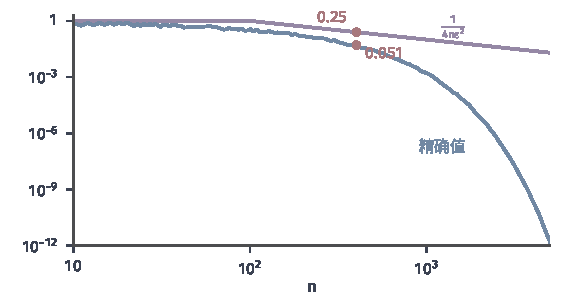
\includegraphics[width=96mm]{figures/07-probability/03-probability-limits/matplotlib/lln-wlln-chebyshev/figure.pdf}
 \caption{均匀硬币的频率偏离$1/2$至少$0.05$的概率，双对数坐标。蓝线为二项分布的精确值，紫线为Chebyshev界$\min\{1,1/(4n\varepsilon^2)\}$，$\varepsilon=0.05$；红点标出$n=400$处的两个值。}
 \label{fig:lln-wlln-chebyshev}
\end{BookInlineFigure}

\paragraph{速度依赖二阶矩}
式~\eqref{eq:lln-wlln-chebyshev}的$1/n$速度来自方差有限这一假设。只知道一阶矩有限时，Chebyshev不等式无法使用，一般也得不到这样的速度：下一小节的Pareto例子中，样本平均的路径时有大的跳跃，靠近均值的过程明显更慢。

\subsection{可积情形}
\label{sec:lln-wlln-integrable}

很多分布均值有限而方差无穷。第~\ref{chap:tail-probabilities}章的Pareto分布，密度为$\alpha x^{-\alpha-1}$（$x\geq1$），取$\alpha=1.5$时
\[
 \mathbb{E}[X]=\int_1^{\infty}x\cdot1.5x^{-2.5}\,\mathrm{d}x=3,\qquad \mathbb{E}[X^2]=\int_1^{\infty}1.5x^{-0.5}\,\mathrm{d}x=\infty .
\]
这时$\operatorname{Var}(\bar{X}_n)=\infty$，Chebyshev不等式无从下手。平均仍应抹平波动，困难在于偶尔出现的大值。办法是先截断：截断后的部分有界，可以用上一小节；被截掉的部分出现得少，用一阶矩控制。

\begin{theorem}[可积情形的弱大数律]
\label{thm:lln-wlln-integrable}
设$X_1,X_2,\dots$独立同分布，$\mathbb{E}[\lvert X_1\rvert]<\infty$，$\mu=\mathbb{E}[X_1]$。则$\bar{X}_n\xrightarrow{\mathbb{P}}\mu$。
\end{theorem}

\begin{proof}
固定$c>0$，把每项分成截断部分与被截掉的部分：
\[
 Y_k=X_k\mathbf{1}_{\{\lvert X_k\rvert\leq c\}},\qquad Z_k=X_k-Y_k=X_k\mathbf{1}_{\{\lvert X_k\rvert>c\}} ,
\]
并记
\[
 \mu_c=\mathbb{E}[Y_1],\qquad \tau(c)=\mathbb{E}\bigl[\lvert X_1\rvert\mathbf{1}_{\{\lvert X_1\rvert>c\}}\bigr]=\mathbb{E}[\lvert Z_1\rvert] .
\]
$\tau(c)$是截掉部分的平均大小。由$\mu=\mu_c+\mathbb{E}[Z_1]$，样本平均的偏差拆成三项：
\[
 \bar{X}_n-\mu=\bigl(\bar{Y}_n-\mu_c\bigr)+\bar{Z}_n-\mathbb{E}[Z_1] ,
\]
其中$\bar{Y}_n$、$\bar{Z}_n$是$Y_k$、$Z_k$的平均。最后一项满足$\lvert\mathbb{E}[Z_1]\rvert\leq\tau(c)$。

固定$\varepsilon>0$，并先假设$c$足够大，使$\tau(c)<\varepsilon/3$。若$\lvert\bar{X}_n-\mu\rvert\geq\varepsilon$，则前两项中至少有一项的绝对值不小于$\varepsilon/3$，所以
\[
 \mathbb{P}\bigl(\lvert\bar{X}_n-\mu\rvert\geq\varepsilon\bigr)\leq\mathbb{P}\bigl(\lvert\bar{Y}_n-\mu_c\rvert\geq\tfrac{\varepsilon}{3}\bigr)+\mathbb{P}\bigl(\lvert\bar{Z}_n\rvert\geq\tfrac{\varepsilon}{3}\bigr) .
\]

第一项是有界变量的平均。$Y_k$独立同分布，且$\lvert Y_1\rvert\leq c$，所以
\[
 \operatorname{Var}(Y_1)\leq\mathbb{E}[Y_1^2]\leq c\,\mathbb{E}[\lvert Y_1\rvert]\leq c\,\mathbb{E}[\lvert X_1\rvert] .
\]
由定理~\ref{thm:lln-wlln-variance}，第一项不超过$9c\,\mathbb{E}[\lvert X_1\rvert]/(n\varepsilon^2)$。第二项用Markov不等式。由三角不等式与同分布，
\[
 \mathbb{E}\bigl[\lvert\bar{Z}_n\rvert\bigr]\leq\frac1n\sum_{k=1}^{n}\mathbb{E}\bigl[\lvert Z_k\rvert\bigr]=\tau(c) ,
\]
所以第二项不超过$3\tau(c)/\varepsilon$。合起来，
\begin{equation}
 \mathbb{P}\bigl(\lvert\bar{X}_n-\mu\rvert\geq\varepsilon\bigr)\leq\frac{9c\,\mathbb{E}[\lvert X_1\rvert]}{n\varepsilon^2}+\frac{3\tau(c)}{\varepsilon} .
 \label{eq:lln-wlln-truncation-bound}
\end{equation}

现在按顺序取极限。先固定$c$令$n\to\infty$，第一项趋于零，得到
\[
 \limsup_{n\to\infty}\mathbb{P}\bigl(\lvert\bar{X}_n-\mu\rvert\geq\varepsilon\bigr)\leq\frac{3\tau(c)}{\varepsilon} .
\]
左边与$c$无关。再令$c\to\infty$：$\lvert X_1\rvert\mathbf{1}_{\{\lvert X_1\rvert>c\}}$逐点趋于零，且被可积的$\lvert X_1\rvert$控制，由支配收敛定理$\tau(c)\to0$。所以左边的上极限为零。
\end{proof}

\paragraph{两个极限的顺序}
式~\eqref{eq:lln-wlln-truncation-bound}的两项此消彼长。截断水平$c$越高，被截掉的部分越小，第二项越小；但留下的部分取值范围越宽，第一项越大。对固定的$n$，令$c\to\infty$会使第一项发散，所以必须先让$n$增大，再放大$c$。等价地说，有用的截断水平要随样本量一起增长，但增长得比$n$慢。

用$\alpha=1.5$的Pareto分布具体看这种权衡。截掉部分的平均大小为
\[
 \tau(c)=\int_c^{\infty}x\cdot1.5x^{-2.5}\,\mathrm{d}x=3c^{-1/2},\qquad c\geq1 ,
\]
截断变量的二阶矩也可以精确算出，
\[
 \mathbb{E}[Y_1^2]=\int_1^c x^2\cdot1.5x^{-2.5}\,\mathrm{d}x=3(\sqrt{c}-1) ,
\]
比证明中用的$c\,\mathbb{E}[X_1]=3c$小得多。取$\varepsilon=1$，用精确的二阶矩代替$c\,\mathbb{E}[\lvert X_1\rvert]$，上界成为
\[
 \frac{27(\sqrt{c}-1)}{n}+\frac{9}{\sqrt{c}},\qquad c>81 ,
\]
其中$c>81$保证$\tau(c)<1/3$。

图~\ref{fig:lln-truncation-tradeoff}(a)画出被截掉的部分：曲线$xf(x)$下$c$右侧的面积就是$\tau(c)$。图(b)画出不同$n$下的总上界。$n=10^4$时最佳截断约为$c\approx3.4\times10^3$，上界约为$0.31$；$n=10^6$时最佳截断移到$c\approx3.3\times10^5$，上界降到约$0.031$。最佳截断水平随$n$增长，上界随之下降。

\begin{BookInlineFigure}
 \centering
 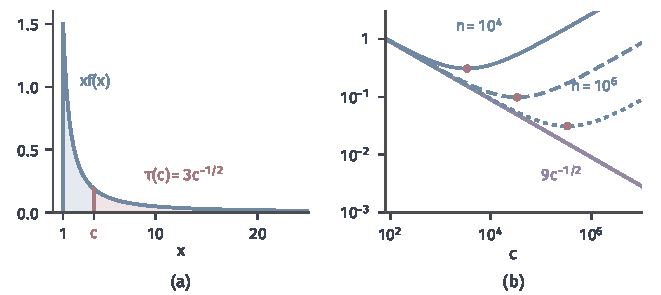
\includegraphics[width=112mm]{figures/07-probability/03-probability-limits/matplotlib/lln-truncation-tradeoff/figure.pdf}
 \caption{$\alpha=1.5$的Pareto分布在弱大数律证明中的截断权衡。(a)求均值的被积函数$xf(x)=1.5x^{-1.5}$（蓝线），截断水平$c=4$左侧为保留部分（浅蓝），右侧为截掉部分（浅红），右侧面积为$\tau(4)=1.5$；(b)$\varepsilon=1$时的上界$27(\sqrt{c}-1)/n+9c^{-1/2}$，蓝色实线、虚线、点线分别对应$n=10^4,10^5,10^6$，红点为各自的最小值，紫线为与$n$无关的第二项$9c^{-1/2}$，双对数坐标。}
 \label{fig:lln-truncation-tradeoff}
\end{BookInlineFigure}

\paragraph{平均意义下的收敛}
同一个截断论证还给出$L^1$收敛。由三角不等式，并对$W=\bar{Y}_n-\mu_c$用一阶绝对矩不超过二阶矩的平方根，
\[
 \mathbb{E}\bigl[\lvert\bar{X}_n-\mu\rvert\bigr]\leq\sqrt{\operatorname{Var}(\bar{Y}_n)}+\mathbb{E}[\lvert\bar{Z}_n\rvert]+\tau(c)\leq\sqrt{\frac{c\,\mathbb{E}[\lvert X_1\rvert]}{n}}+2\tau(c) .
\]
同样先令$n\to\infty$再令$c\to\infty$，得到$\bar{X}_n\xrightarrow{L^{1}}\mu$。

\paragraph{可积不是有限方差}
定理只要求$\mathbb{E}[\lvert X_1\rvert]<\infty$。图~\ref{fig:lln-pareto-cauchy}(a)是$\alpha=1.5$的Pareto样本平均：五条路径最终都靠近$\mu=3$，但不时被一个大观测猛地抬高，再慢慢回落。$n=10^5$时五个平均分别约为$3.00$、$2.98$、$2.97$、$2.97$、$2.92$，多数略低于$3$，因为把平均拉回$3$的正是那些尚未出现的稀有大值。

如果连一阶矩都没有，平均就不再稳定。图(b)是标准Cauchy分布的样本平均，路径不断被新的极端值拉到别处。第~\ref{chap:weak-convergence-of-distributions}章用特征函数可以证明，独立标准Cauchy变量的平均$\bar{X}_n$对每个$n$仍服从标准Cauchy分布，于是
\[
 \mathbb{P}\bigl(\lvert\bar{X}_n\rvert\geq1\bigr)=1-\frac{2}{\pi}\arctan1=\frac12\quad\text{对所有}\ n ,
\]
不趋于零。平均$n$个观测与只看一个观测效果相同，抹平机制完全失效。

\begin{BookInlineFigure}
 \centering
 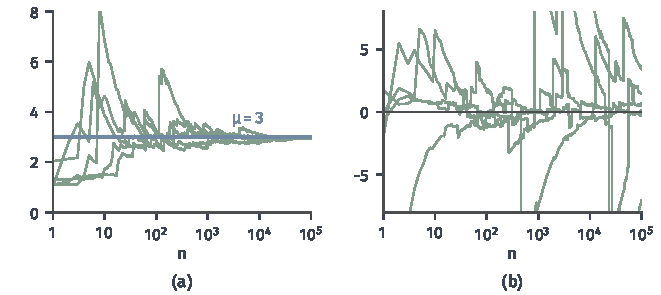
\includegraphics[width=112mm]{figures/07-probability/03-probability-limits/matplotlib/lln-pareto-cauchy/figure.pdf}
 \caption{重尾样本的平均，每图五条路径，横轴为对数刻度。(a)$\alpha=1.5$的Pareto分布（种子$13$），均值$\mu=3$（蓝线），方差无穷；(b)标准Cauchy分布（种子$14$），均值不存在，纵轴截在$[-8,8]$。}
 \label{fig:lln-pareto-cauchy}
\end{BookInlineFigure}


\section{强大数律}
\label{sec:lln-strong-law}

弱大数律对每个固定的$n$说：偏差超过$\varepsilon$的路径只占很小的比例。它没有说同一条路径以后不会再出界。图~\ref{fig:lln-weak-vs-strong}画出$40$条硬币频率路径（种子$21$）与带$0.5\pm0.05$。在$n=400$处只有$3$条在带外，这是弱大数律描述的事情。另一个问题是：沿着一条固定的路径往后看，它是否从某一步起永远留在带内？图中红点标出每条路径在$n\leq2000$内最后一次出带的时刻，最晚的在$n=727$。

\begin{BookInlineFigure}
 \centering
 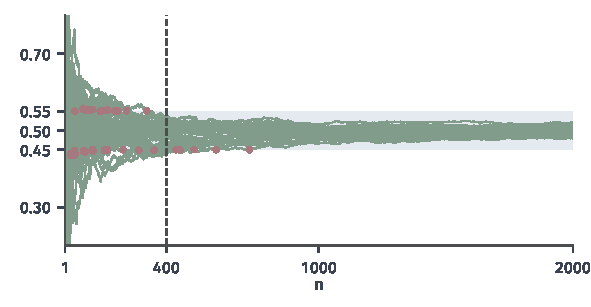
\includegraphics[width=100mm]{figures/07-probability/03-probability-limits/matplotlib/lln-weak-vs-strong/figure.pdf}
 \caption{$40$条均匀硬币的频率路径（绿线，种子$21$），$n\leq2000$。浅蓝带为$0.5\pm0.05$；红点为各路径在图示范围内最后一次位于带外的时刻；虚线标出$n=400$。}
 \label{fig:lln-weak-vs-strong}
\end{BookInlineFigure}

图只能显示有限的范围，“永远留在带内”是关于整条无限路径的断言。把它写成定义，就是几乎必然收敛。

\begin{definition}[强大数律]
\label{def:lln-strong-law}
设随机变量列$X_1,X_2,\dots$各项可积且有共同的均值$\mu$。若$\bar{X}_n\xrightarrow{\mathrm{a.s.}}\mu$，即
\begin{equation}
 \mathbb{P}\Bigl(\lim_{n\to\infty}\bar{X}_n=\mu\Bigr)=1 ,
 \label{eq:lln-strong-law}
\end{equation}
则称这列变量满足\term{强大数律}（strong law of large numbers）。
\end{definition}

由第~\ref{chap:random-variable-convergence}章，几乎必然收敛蕴含依概率收敛，所以强律推出弱律。反过来不能直接升级。Chebyshev界$\sigma^2/(n\varepsilon^2)$对$n$求和发散，Borel–Cantelli引理无从使用：每个时刻出界的概率虽小，加起来却是无穷，不能排除无穷多次出界。要证明强律，需要同时控制所有后续时刻，这正是前两节为随机级数建立的工具。思路是先证明加权级数$\sum_k(X_k-\mu)/k$收敛，再把级数的收敛翻译成平均的收敛。

\subsection{从级数收敛到平均收敛}
\label{sec:lln-series-to-average}

先看一个确定的问题。设实数$x_1,x_2,\dots$使$\sum_kx_k/k$收敛，能否推出$\frac1n\sum_{k\leq n}x_k\to0$？直觉是：级数收敛说明$x_k$按自身大小$k$折算后的累计有限，而前$n$项的总和除以更大的$n$时，早期各项被压小，后期各项又已经很小。

\begin{lemma}[Kronecker引理]
\label{lem:lln-kronecker}
设$0<b_1\leq b_2\leq\cdots$，$b_n\to\infty$，实数列$(x_k)$使$\sum_kx_k/b_k$收敛。则
\begin{equation}
 \lim_{n\to\infty}\frac{1}{b_n}\sum_{k=1}^{n}x_k=0 .
 \label{eq:lln-kronecker}
\end{equation}
\end{lemma}

这个结论称为\term{Kronecker引理}（Kronecker's lemma）。证明用\term{分部求和}（summation by parts），即离散形式的分部积分。

\begin{proof}
记$s_0=0$，$s_n=\sum_{k\leq n}x_k/b_k$，由假设$s_n\to s$。于是$x_k=b_k(s_k-s_{k-1})$。分部求和，把$b_k$与差分$s_k-s_{k-1}$交换位置：
\[
 \sum_{k=1}^{n}x_k=\sum_{k=1}^{n}b_k(s_k-s_{k-1})=b_ns_n-\sum_{k=1}^{n-1}(b_{k+1}-b_k)s_k .
\]
这个恒等式可以按$s_k$的系数逐项核对：$s_n$的系数是$b_n$，$k<n$时$s_k$的系数是$b_k-b_{k+1}$。两边除以$b_n$，
\begin{equation}
 \frac{1}{b_n}\sum_{k=1}^{n}x_k=s_n-\frac{1}{b_n}\sum_{k=1}^{n-1}(b_{k+1}-b_k)s_k .
 \label{eq:lln-abel-identity}
\end{equation}

右边第二项是$s_1,\dots,s_{n-1}$的加权平均，权重$w_{n,k}=(b_{k+1}-b_k)/b_n\geq0$，总和为$(b_n-b_1)/b_n\to1$。下面说明它趋于$s$。给定$\eta>0$，取$N$使$k\geq N$时$\lvert s_k-s\rvert<\eta$。则$n>N$时
\[
 \Bigl\lvert\sum_{k=1}^{n-1}w_{n,k}(s_k-s)\Bigr\rvert\leq\frac{1}{b_n}\sum_{k=1}^{N-1}(b_{k+1}-b_k)\lvert s_k-s\rvert+\eta .
\]
右边第一项的分子与$n$无关，$b_n\to\infty$时趋于零。所以上极限不超过$\eta$，而$\eta$任意。再由$\sum_kw_{n,k}s=s(b_n-b_1)/b_n\to s$，第二项趋于$s$。式~\eqref{eq:lln-abel-identity}的右边趋于$s-s=0$。
\end{proof}

$b_n=n$时，$b_{k+1}-b_k=1$，式~\eqref{eq:lln-abel-identity}的加权平均就是$\frac1n\sum_{k<n}s_k$，即部分和序列的\term{Cesàro平均}（Cesàro mean）。证明的核心是：收敛序列的Cesàro平均收敛到同一极限，而样本平均恰好是原序列与它的Cesàro平均之差。

\paragraph{一个确定的例子}
取$x_k=(-1)^{k+1}\sqrt{k}$。$\sum_kx_k/k=\sum_k(-1)^{k+1}/\sqrt{k}$是交错级数，项的绝对值单调趋于零，所以收敛，和约为$0.6049$。由Kronecker引理，
\[
 \frac1n\sum_{k=1}^{n}(-1)^{k+1}\sqrt{k}\to0 .
\]
直接计算，$n=100,1000,10000$时这个平均分别约为$-0.0463$、$-0.0154$、$-0.0050$，大致与$-1/(2\sqrt{n})$相当。注意$x_k$本身无界，$\lvert x_k\rvert=\sqrt{k}\to\infty$，平均趋于零完全来自正负抵消。

图~\ref{fig:lln-kronecker}画出式~\eqref{eq:lln-abel-identity}中的两项。图(a)中蓝线$s_n$来回振荡地收敛，黄线是它的Cesàro平均，平滑地趋于同一极限；图(b)是二者之差，即样本平均，它被夹在$\pm1/(2\sqrt{n})$之间趋于零。

\begin{BookInlineFigure}
 \centering
 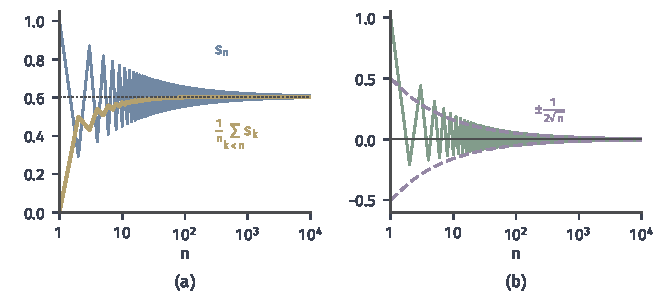
\includegraphics[width=112mm]{figures/07-probability/03-probability-limits/matplotlib/lln-kronecker/figure.pdf}
 \caption{Kronecker引理的恒等式~\eqref{eq:lln-abel-identity}，$b_n=n$，$x_k=(-1)^{k+1}\sqrt{k}$，横轴为对数刻度。(a)$s_n=\sum_{k\leq n}x_k/k$（蓝线）与其Cesàro平均$\frac1n\sum_{k<n}s_k$（黄线），点线为极限$0.6049$；(b)二者之差$\frac1n\sum_{k\leq n}x_k$（绿线）与$\pm1/(2\sqrt{n})$（紫色虚线）。}
 \label{fig:lln-kronecker}
\end{BookInlineFigure}

\paragraph{用到随机变量上}
Kronecker引理是关于实数列的确定性结论。用于随机变量时，先找一个概率为一的事件，在它上面级数收敛，再对其中每个样本点分别使用引理。下面的定理就是这样得到的。

\begin{theorem}[方差加权可和时的强大数律]
\label{thm:lln-kolmogorov-criterion}
设$X_1,X_2,\dots$相互独立，$\mu_k=\mathbb{E}[X_k]$，$\sigma_k^2=\operatorname{Var}(X_k)$，且
\begin{equation}
 \sum_{k=1}^{\infty}\frac{\sigma_k^2}{k^2}<\infty .
 \label{eq:lln-kolmogorov-criterion}
\end{equation}
则
\begin{equation}
 \frac{\tilde{S}_n}{n}=\frac1n\sum_{k=1}^{n}(X_k-\mu_k)\xrightarrow{\mathrm{a.s.}}0 .
 \label{eq:lln-kolmogorov-slln}
\end{equation}
\end{theorem}

\begin{proof}
变量$(X_k-\mu_k)/k$相互独立，均值为零，方差为$\sigma_k^2/k^2$。由条件~\eqref{eq:lln-kolmogorov-criterion}与定理~\ref{thm:lln-variance-series}，存在概率为一的事件$\Omega_0$，在其上级数$\sum_k(X_k-\mu_k)/k$收敛。对每个$\omega\in\Omega_0$，对实数列$x_k=X_k(\omega)-\mu_k$与$b_k=k$用引理~\ref{lem:lln-kronecker}，得到$\tilde{S}_n(\omega)/n\to0$。
\end{proof}

两个特例直接可用。第一，独立同分布且方差$\sigma^2$有限时，$\sum_k\sigma^2/k^2<\infty$，所以$\bar{X}_n\xrightarrow{\mathrm{a.s.}}\mu$：有限方差的强大数律成立。第二，第~\ref{sec:lln-normalization}小节的分段Bernoulli变量满足$\sigma_k^2=p_k(1-p_k)\leq1/4$，条件成立，所以$(S_n-\sum_{k\leq n}p_k)/n\to0$几乎必然成立，这正是图~\ref{fig:lln-varying-means}(b)显示的现象。各项分布不同，样本平均本身却不收敛，强律的正确形式是中心化平均趋于零。

\subsection{独立同分布可积情形}
\label{sec:lln-slln-integrable}

最后去掉有限方差的假设。与弱律一样，办法是截断；不同的是，截断水平这次随项数增长。

\begin{theorem}[强大数律]
\label{thm:lln-slln}
设$X_1,X_2,\dots$独立同分布，$\mathbb{E}[\lvert X_1\rvert]<\infty$，$\mu=\mathbb{E}[X_1]$。则$\bar{X}_n\xrightarrow{\mathrm{a.s.}}\mu$。
\end{theorem}

\begin{proof}
对每个$k$，在水平$k$处截断：
\[
 Y_k=X_k\mathbf{1}_{\{\lvert X_k\rvert\leq k\}} .
\]
$Y_k$是独立变量$X_k$的函数，所以$Y_1,Y_2,\dots$相互独立，但截断水平不同，它们不再同分布。把样本平均的偏差拆成三项：
\[
 \bar{X}_n-\mu=\frac1n\sum_{k=1}^{n}(X_k-Y_k)+\frac1n\sum_{k=1}^{n}\bigl(Y_k-\mathbb{E}[Y_k]\bigr)+\Bigl(\frac1n\sum_{k=1}^{n}\mathbb{E}[Y_k]-\mu\Bigr) .
\]
下面分三步证明每一项几乎必然趋于零。

\emph{第一步：大项只出现有限次。}$X_k$与$X_1$同分布，所以$X_k\neq Y_k$的概率是$\mathbb{P}(\lvert X_1\rvert>k)$。函数$t\mapsto\mathbb{P}(\lvert X_1\rvert>t)$不增，所以它在$t=k$处的值不超过它在区间$[k-1,k]$上的平均：
\[
 \mathbb{P}(\lvert X_1\rvert>k)\leq\int_{k-1}^{k}\mathbb{P}(\lvert X_1\rvert>t)\,\mathrm{d}t .
\]
对$k$求和，再由第~\ref{chap:tail-probabilities}章的尾积分公式，
\[
 \sum_{k=1}^{\infty}\mathbb{P}(\lvert X_1\rvert>k)\leq\int_0^{\infty}\mathbb{P}(\lvert X_1\rvert>t)\,\mathrm{d}t=\mathbb{E}[\lvert X_1\rvert]<\infty .
\]
由Borel–Cantelli引理，几乎必然只有有限个$k$使$X_k\neq Y_k$。在这样的样本点上，$\sum_{k\leq n}(X_k-Y_k)$从某项起不再变化，除以$n$后趋于零。

\emph{第二步：截断均值趋于$\mu$。}由同分布，$\mathbb{E}[Y_k]$等于$X_1\mathbf{1}_{\{\lvert X_1\rvert\leq k\}}$的期望。这个随机变量逐点趋于$X_1$，且被可积的$\lvert X_1\rvert$控制，由支配收敛定理$\mathbb{E}[Y_k]\to\mu$。收敛数列的Cesàro平均收敛到同一极限（这是Kronecker引理证明中的第二步，取$b_n=n$），所以第三项趋于零。

\emph{第三步：截断波动的加权方差可和。}要对$Y_k-\mathbb{E}[Y_k]$用定理~\ref{thm:lln-kolmogorov-criterion}，需检查$\sum_k\operatorname{Var}(Y_k)/k^2<\infty$。由$\operatorname{Var}(Y_k)\leq\mathbb{E}[Y_k^2]$，并交换非负项的求和与期望，
\[
 \sum_{k=1}^{\infty}\frac{\operatorname{Var}(Y_k)}{k^2}\leq\sum_{k=1}^{\infty}\frac{\mathbb{E}\bigl[X_1^2\mathbf{1}_{\{\lvert X_1\rvert\leq k\}}\bigr]}{k^2}=\mathbb{E}\Bigl[X_1^2\sum_{k\geq\lvert X_1\rvert,\,k\geq1}\frac{1}{k^2}\Bigr] .
\]
对实数$x\neq0$，记$m=\lceil\lvert x\rvert\rceil\geq1$，则$m\geq\lvert x\rvert$，并且
\[
 \sum_{k\geq m}\frac{1}{k^2}\leq\frac{1}{m^2}+\int_m^{\infty}\frac{\mathrm{d}t}{t^2}=\frac{1}{m^2}+\frac1m\leq\frac2m\leq\frac{2}{\lvert x\rvert} .
\]
所以期望内的量不超过$x^2\cdot2/\lvert x\rvert=2\lvert x\rvert$；$x=0$时它为零。于是
\[
 \sum_{k=1}^{\infty}\frac{\operatorname{Var}(Y_k)}{k^2}\leq2\,\mathbb{E}[\lvert X_1\rvert]<\infty .
\]
由定理~\ref{thm:lln-kolmogorov-criterion}，第二项几乎必然趋于零。

三项各在一个概率为一的事件上趋于零，三个事件的交概率仍为一，定理得证。
\end{proof}

\paragraph{为什么截断水平取$k$}
若在固定水平$c$截断，被截掉的大值以固定概率$\mathbb{P}(\lvert X_1\rvert>c)>0$反复出现，无穷多次，第一步失效。若截断水平增长得太快，截断变量的方差太大，第三步的级数可能发散。水平$k$恰好使两边都只用到一阶矩：第一步的级数$\sum_k\mathbb{P}(\lvert X_1\rvert>k)$与第三步的级数都被$\mathbb{E}[\lvert X_1\rvert]$控制。

用$\alpha=1.5$的Pareto分布核对两个级数。第一步，$\mathbb{P}(X_1>k)=k^{-1.5}$，
\[
 \sum_{k=1}^{\infty}k^{-1.5}\approx2.612\leq\mathbb{E}[X_1]=3 .
\]
第三步，$\mathbb{E}[Y_k^2]=3(\sqrt{k}-1)$，
\[
 \sum_{k=1}^{\infty}\frac{3(\sqrt{k}-1)}{k^2}\approx2.896\leq2\,\mathbb{E}[X_1]=6 .
\]
图~\ref{fig:lln-truncation-diagonal}画出一组$2000$个Pareto观测（种子$17$）与对角线$x=k$。落在对角线上方、被截断改动的只有$5$个点，位于$k=1,2,10,19,335$；按第一步的级数，期望个数约为$2.57$。$k$越大，越过$k$越难，这些点集中在开头。

\begin{BookInlineFigure}
 \centering
 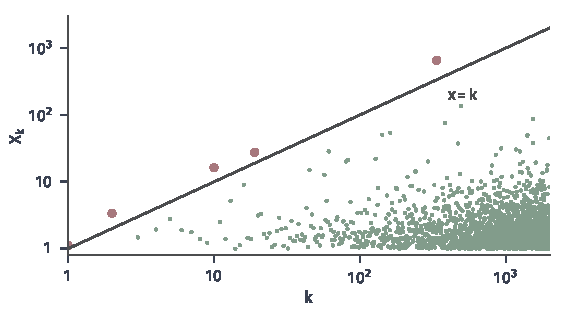
\includegraphics[width=96mm]{figures/07-probability/03-probability-limits/matplotlib/lln-truncation-diagonal/figure.pdf}
 \caption{$\alpha=1.5$的Pareto样本$X_1,\dots,X_{2000}$（种子$17$），双对数坐标。深灰直线为截断水平$x=k$；红点为$X_k>k$、被截断改动的观测，绿点为其余观测。}
 \label{fig:lln-truncation-diagonal}
\end{BookInlineFigure}

\paragraph{可积条件不能去掉}
对独立同分布序列，可积性不仅充分，而且必要。设$\mathbb{E}[\lvert X_1\rvert]=\infty$。与第一步反方向比较，$\mathbb{P}(\lvert X_1\rvert>k)$不小于生存函数在$[k,k+1]$上的平均，所以
\[
 \sum_{k=1}^{\infty}\mathbb{P}(\lvert X_k\rvert>k)\geq\int_1^{\infty}\mathbb{P}(\lvert X_1\rvert>t)\,\mathrm{d}t\geq\mathbb{E}[\lvert X_1\rvert]-1=\infty .
\]
事件$\{\lvert X_k\rvert>k\}$相互独立，由Borel–Cantelli引理的第二部分，几乎必然有无穷多个$k$使$\lvert X_k\rvert/k>1$。另一方面，若$\bar{X}_n$收敛到有限数$L$，则
\[
 \frac{X_n}{n}=\bar{X}_n-\frac{n-1}{n}\bar{X}_{n-1}\to L-L=0 .
\]
两者矛盾，所以$\bar{X}_n$收敛到有限极限的概率为零。图~\ref{fig:lln-pareto-cauchy}(b)的Cauchy路径就是这种情形。

\paragraph{弱律与强律的比较}
表~\ref{tab:lln-weak-strong}把两种大数律放在一起。对独立同分布序列，强律的条件恰好是可积；弱律的结论较弱，它在比可积稍弱的尾部条件下仍可能对适当的中心成立，读者可查阅~\scite{math-kallenberg2021probability}。

\begin{BookInlineTable}
 \centering
 \caption{弱大数律与强大数律（独立同分布，$\mu=\mathbb{E}[X_1]$）。}
 \label{tab:lln-weak-strong}
 \begin{tabular}{lll}
  \toprule
  & 弱大数律 & 强大数律\\
  \midrule
  结论 & 依概率收敛 & 几乎必然收敛\\
  控制对象 & 每个固定时刻 & 整条路径的尾部\\
  有限方差时 & Chebyshev不等式 & 加权级数与Kronecker引理\\
  只有一阶矩时 & 固定水平截断 & 水平随$k$增长的截断\\
  有限样本误差 & 有方差时为$\sigma^2/(n\varepsilon^2)$ & 本身不给速度\\
  \bottomrule
 \end{tabular}
\end{BookInlineTable}

强律回答的是“最终会不会稳定”，它本身不说明何时稳定，也不给出有限样本的误差。对固定的$n$，误差大小仍要靠Chebyshev不等式或更强的集中不等式估计；后者对有界变量给出指数衰减的界，可参考\BookChapterRef{chap:finite-sample-error-bounds}{卷八第4章“有限样本的误差上界”}。


\section{经验平均的应用}
\label{sec:lln-applications}

实际计算中出现的许多量都是平均：一个事件发生的频率、一个函数在观测上的平均、样本的各阶矩。要对它们用大数律，先把它们写成某列随机变量的样本平均，再逐项核对三件事：这列变量是否独立同分布，被平均的函数是否在看到数据之前就已固定，它的期望是否绝对可积。

设$X_1,X_2,\dots$独立同分布，取值于集合$\mathcal{X}$（例如$\mathbb{R}$或$\mathbb{R}^d$），共同分布为$P_X$。本节只讨论预先给定的事件和函数；在看到数据之后再挑选函数或事件，需要对一整族同时成立的保证，那是统计推断的问题。

\subsection{事件频率}
\label{sec:lln-frequency}

第~\ref{chap:classical-probability}章用重复试验中的相对频率解释概率，并在模拟中看到频率稳定在概率附近。现在可以说明它为什么稳定。

对固定的事件$A\subseteq\mathcal{X}$（要求$A$是可测集，即$\{X_1\in A\}$是事件），令
\begin{equation}
 f_n(A)=\frac{1}{n}\sum_{i=1}^{n}\mathbf{1}_{A}(X_i) ,
 \label{eq:lln-frequency}
\end{equation}
即前$n$次观测中落入$A$的比例。示性变量$\mathbf{1}_A(X_i)$独立同分布，服从$\operatorname{Bern}(p)$，其中$p=\mathbb{P}(X_1\in A)$。它们取值于$\{0,1\}$，均值为$p$，方差为$p(1-p)$。

\begin{theorem}[频率的大数律]
\label{thm:lln-frequency}
设$X_1,X_2,\dots$独立同分布，$A$是固定的可测集，$p=\mathbb{P}(X_1\in A)$。则$f_n(A)\xrightarrow{\mathrm{a.s.}}p$，并且对每个$\varepsilon>0$与每个$n$，
\begin{equation}
 \mathbb{P}\bigl(\lvert f_n(A)-p\rvert\geq\varepsilon\bigr)\leq\frac{p(1-p)}{n\varepsilon^2}\leq\frac{1}{4n\varepsilon^2} .
 \label{eq:lln-frequency-bound}
\end{equation}
\end{theorem}

\begin{proof}
示性变量有界，从而可积且方差有限。对它们用定理~\ref{thm:lln-slln}得到几乎必然收敛，用定理~\ref{thm:lln-wlln-variance}得到第一个不等式。第二个不等式来自$p(1-p)\leq1/4$。
\end{proof}

这个结论称为Borel强大数律，它是概率的频率解释的数学内容。以骰子为例，令$A$为“掷出$6$点”，则几乎每一串掷骰记录中$6$点的比例都趋于$1/6$。这里的“几乎每一串”有确切含义：例外的记录（例如永远掷出$6$点）当然可以写下来，但它们的全体概率为零。

\paragraph{随机投点估面积}
频率还可以用来计算面积。设$U,V$独立且都服从$\operatorname{Unif}(0,1)$，事件$A=\{U^2+V^2\leq1\}$是单位正方形中的四分之一圆盘，概率等于它的面积$\pi/4$。在正方形中独立投点，落入圆盘的比例几乎必然趋于$\pi/4$，所以$4f_n(A)\to\pi$。这种用随机样本的平均计算积分的方法称为Monte Carlo方法。

图~\ref{fig:lln-monte-carlo}(a)画出一次投点（种子$31$）的前$400$个点，其中$316$个落在圆内，给出估计$4\times316/400=3.16$。图(b)画出五次独立投点的估计路径，$n=10^4$时它们落在$3.130$到$3.156$之间。式~\eqref{eq:lln-frequency-bound}给出估计的标准差
\[
 4\sqrt{\frac{p(1-p)}{n}}=4\sqrt{\frac{0.7854\times0.2146}{10^4}}\approx0.016 ,
\]
与五个估计的散布相符。误差怎样随样本数缩小、怎样减小它，是第~\ref{chap:monte-carlo-integration-error}章与第~\ref{chap:variance-reduction}章的内容。

\begin{BookInlineFigure}
 \centering
 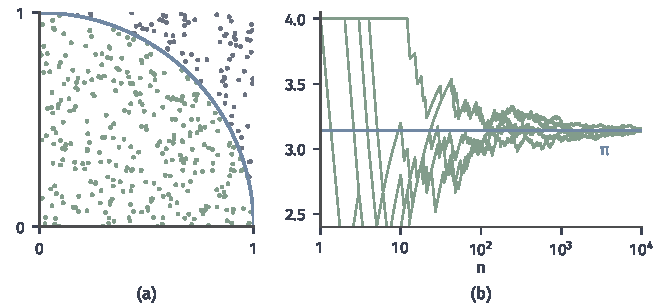
\includegraphics[width=112mm]{figures/07-probability/03-probability-limits/matplotlib/lln-monte-carlo/figure.pdf}
 \caption{用频率估计四分之一圆的面积。(a)单位正方形中的前$400$个均匀点（种子$31$），绿点落在四分之一圆内，灰点落在圆外，蓝线为圆弧；(b)五次独立投点（种子$31$至$35$）的估计$4f_n(A)$（绿线）与$\pi$（蓝线），横轴为对数刻度。}
 \label{fig:lln-monte-carlo}
\end{BookInlineFigure}

\paragraph{固定事件与事件族}
定理~\ref{thm:lln-frequency}对每个固定的$A$给出一个概率为一的事件$\Omega_A$，在其上$f_n(A)\to p$。不同的$A$对应的例外集不同。对可数个事件$A_1,A_2,\dots$，可数个零概率集的并仍是零概率集，所以几乎必然地，$f_n(A_j)\to\mathbb{P}(X_1\in A_j)$对所有$j$同时成立。例如所有端点为有理数的区间可以同时处理。

对所有事件同时成立却是错的。设$X_i$服从$\operatorname{Unif}(0,1)$，取事件$A=\{X_1,\dots,X_n\}$，即观测到的那些点组成的有限集。它的频率是$f_n(A)=1$，概率却是$\mathbb{P}(X_1\in A)=0$，因为连续分布不给单点任何质量。图~\ref{fig:lln-finite-event}画出了这种情形。于是对每个$n$和每个样本点，
\[
 \sup_{A}\bigl\lvert f_n(A)-\mathbb{P}(X_1\in A)\bigr\rvert=1 .
\]

\begin{BookInlineFigure}
 \centering
 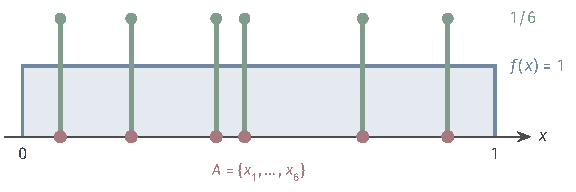
\includegraphics[width=98mm]{figures/07-probability/03-probability-limits/tikz/lln-finite-event/figure.pdf}
 \caption{均匀分布（蓝色，密度为$1$）与六个观测点的经验质量（绿色竖线，每点$1/6$）。由观测点组成的事件$A=\{x_1,\dots,x_6\}$（红点）频率为$1$，在均匀分布下的概率为$0$。}
 \label{fig:lln-finite-event}
\end{BookInlineFigure}

问题出在事件依赖于数据。定理中的$A$必须在观测之前固定。对半直线$(-\infty,t]$这样的特殊事件族，频率可以对整族一致收敛，但那需要额外的论证，属于统计推断的内容，见\BookChapterRef{chap:nonparametric-inference}{卷八第2章“非参数分布与函数推断”}。

\subsection{函数平均与样本矩}
\label{sec:lln-function-averages}

频率是函数平均的特例：被平均的函数是示性函数。一般地，取一个固定的函数$g\colon\mathcal{X}\to\mathbb{R}$（要求可测，使$g(X_1)$是随机变量），考虑$\frac1n\sum_{i\leq n}g(X_i)$。

\begin{theorem}[函数平均的大数律]
\label{thm:lln-function-average}
设$X_1,X_2,\dots$独立同分布，$g$可测，$\mathbb{E}[\lvert g(X_1)\rvert]<\infty$。则
\begin{equation}
 \frac{1}{n}\sum_{i=1}^{n}g(X_i)\xrightarrow{\mathrm{a.s.}}\mathbb{E}[g(X_1)] .
 \label{eq:lln-function-average}
\end{equation}
\end{theorem}

\begin{proof}
$g(X_1),g(X_2),\dots$是独立变量的函数，所以相互独立；它们的分布都是$g(X_1)$的分布，所以同分布。由假设它们可积，对它们用定理~\ref{thm:lln-slln}即可。
\end{proof}

条件$\mathbb{E}[\lvert g(X_1)\rvert]<\infty$必须针对$g(X_1)$检查，而不是针对$X_1$。例如$X_1\sim\operatorname{Unif}(0,1)$有界，但$g(x)=1/x$使
\[
 \mathbb{E}[g(X_1)]=\int_0^1\frac{\mathrm{d}x}{x}=\infty ,
\]
定理不能直接使用。这时平均$\frac1n\sum_i1/X_i$几乎必然趋于$+\infty$：对每个$M>0$，$1/X_i\geq\min\{1/X_i,M\}$，后者有界，由定理得
\[
 \liminf_{n\to\infty}\frac1n\sum_{i=1}^{n}\frac{1}{X_i}\geq\mathbb{E}\bigl[\min\{1/X_1,M\}\bigr]\quad\text{几乎必然},
\]
而右边随$M\to\infty$单调增至$\infty$。取$M=1,2,\dots$，可数个例外集的并仍是零概率集。

\paragraph{样本矩}
取$g(x)=x^r$，$r$为正整数，得到$r$阶\term{样本矩}（sample moment）
\[
 m_{n,r}=\frac{1}{n}\sum_{i=1}^{n}X_i^r .
\]
由定理~\ref{thm:lln-function-average}，只要$\mathbb{E}[\lvert X_1\rvert^r]<\infty$，就有$m_{n,r}\to\mathbb{E}[X_1^r]$几乎必然成立。一阶样本矩就是样本平均$\bar{X}_n$。

\paragraph{样本方差}
常用的\term{样本方差}（sample variance）是
\begin{equation}
 S_n^{2}=\frac{1}{n-1}\sum_{i=1}^{n}\bigl(X_i-\bar{X}_n\bigr)^2,\qquad n\geq2 .
 \label{eq:lln-sample-variance}
\end{equation}
这里$S_n^2$是一个新记号，与部分和$S_n$的平方无关；本小节只在这个意义下使用它。它不是单个函数的平均，因为每一项都含有$\bar{X}_n$。先把平方和展开，用$\sum_iX_i=n\bar{X}_n$，
\[
 \sum_{i=1}^{n}(X_i-\bar{X}_n)^2=\sum_{i=1}^{n}X_i^2-2\bar{X}_n\sum_{i=1}^{n}X_i+n\bar{X}_n^2=\sum_{i=1}^{n}X_i^2-n\bar{X}_n^2 .
\]
于是样本方差写成两个样本矩的组合：
\[
 S_n^{2}=\frac{n}{n-1}\bigl(m_{n,2}-\bar{X}_n^2\bigr) .
\]

现在只需$\mathbb{E}[X_1^2]<\infty$。这时$X_1$也可积，由定理~\ref{thm:lln-function-average}，$m_{n,2}\to\mathbb{E}[X_1^2]$与$\bar{X}_n\to\mu$各在一个概率为一的事件上成立。在两个事件的交上，平方与乘积都是连续运算，$n/(n-1)\to1$，所以
\begin{equation}
 S_n^{2}\xrightarrow{\mathrm{a.s.}}\mathbb{E}[X_1^2]-\mu^2=\sigma^2 .
 \label{eq:lln-sample-variance-limit}
\end{equation}

这个结论只用到有限的二阶矩，不需要假设四阶矩有限。四阶矩控制的是$S_n^2$本身的方差，也就是它在$\sigma^2$附近波动的大小；收敛本身不需要它。

用一组具体数据核对公式。掷五次骰子得到$2,5,3,6,1$，则
\[
 \bar{X}_5=\frac{17}{5}=3.4,\qquad m_{5,2}=\frac{4+25+9+36+1}{5}=15 ,
\]
所以
\[
 S_5^2=\frac54\bigl(15-3.4^2\bigr)=\frac54\times3.44=4.3 .
\]
五次观测太少，$4.3$离$\sigma^2=35/12\approx2.917$还很远。图~\ref{fig:lln-sample-variance}(a)是五条长路径（种子$41$），$n=10^5$时样本方差落在$2.903$到$2.924$之间。

图(b)换成自由度$\nu=3$的t分布（种子$42$）。它的方差为$\nu/(\nu-2)=3$，四阶矩却是无穷。样本方差仍然收敛到$3$，但路径不时被一个大观测猛地推高，再慢慢回落，收敛明显比骰子慢。这正说明四阶矩影响的是波动大小，而不是收敛与否。

\begin{BookInlineFigure}
 \centering
 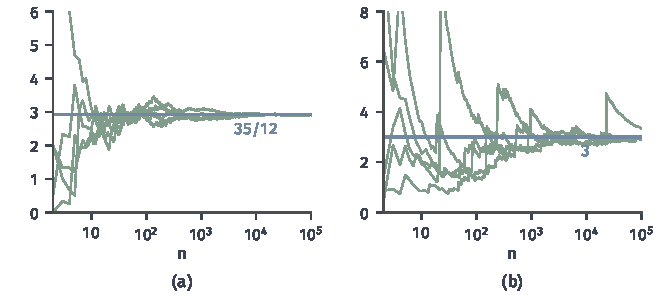
\includegraphics[width=112mm]{figures/07-probability/03-probability-limits/matplotlib/lln-sample-variance/figure.pdf}
 \caption{样本方差$S_n^2$的路径，每图五条（绿线），横轴为对数刻度，蓝线为总体方差。(a)均匀骰子（种子$41$），$\sigma^2=35/12$；(b)自由度$3$的t分布（种子$42$），$\sigma^2=3$，四阶矩无穷。}
 \label{fig:lln-sample-variance}
\end{BookInlineFigure}

\paragraph{适用边界}
本节的结论说明：给定分布与给定函数，经验平均几乎必然趋于相应的期望。它不回答平均以多快的速度接近期望，也不回答在平均附近放大后的误差服从什么分布；前者需要矩或尾部信息，后者是中心极限定理的内容。用样本平均去估计未知的期望、给出可信区间，则是统计推断的问题，由卷八承担。


\section{本章小结}
\label{sec:lln-summary}

本章研究独立随机变量的部分和$S_n$，并区分两个问题：未归一化的累计$\sum_kX_k$是否收敛，以及平均$\bar{X}_n$是否稳定在期望附近。两者用的是同一组工具，各工具解决的环节不同。

\paragraph{部分和的两个基本估计}
独立性使中心化交叉项的期望为零，方差可加，$\operatorname{Var}(S_n)=\sum_k\sigma_k^2$；部分和的散布因此按$\sqrt{n}$增长，样本平均按$1/\sqrt{n}$收窄。Chebyshev不等式只控制固定终点。Kolmogorov最大不等式按首次越过阈值的时刻拆分事件，利用之后增量的独立性与零均值，用同一个终点方差控制整段路径的最大偏离。它需要独立与中心化，两者缺一不可。

\paragraph{随机级数}
最大不等式控制尾段的振荡，于是独立中心化、方差可和的级数几乎必然收敛，同时在$L^2$中收敛。有非零均值时还要单独检查均值级数。方差或均值被罕见大值破坏时，在固定水平截断：大项由超阈值概率可和与Borel–Cantelli引理排除，截断均值由数项级数控制，截断波动由方差可和控制。三系列定理说明这三个条件也是必要的；随机符号级数$\sum_ka_k\varepsilon_k$几乎必然收敛当且仅当$\sum_ka_k^2<\infty$。

\paragraph{两种大数律}
弱大数律回答每个固定时刻偏差的概率。有限方差时Chebyshev不等式给出有限样本的界$\sigma^2/(n\varepsilon^2)$；只有一阶矩时，先固定截断水平、令样本量增大，再放大截断水平。强大数律回答几乎每条路径的最终行为。Kronecker引理把加权级数$\sum_k(X_k-\mu_k)/k$的收敛逐样本地翻译成平均的收敛；对可积的独立同分布序列，按项数$k$截断，使大项只出现有限次、截断方差的加权和被一阶矩控制。可积对强律既充分又必要，Cauchy分布是反例。

\paragraph{使用时核对的条件}
频率、函数平均与样本矩都是独立同分布变量的平均。使用前确认被平均的事件或函数在观测之前固定、相应的期望绝对可积；样本方差的几乎必然收敛只需有限二阶矩。对依赖数据挑选的事件族，单个事件的结论不能直接推广。

大数律确定了平均的极限位置，却没有说明平均在极限附近怎样波动。把偏差$\bar{X}_n-\mu$放大$\sqrt{n}$倍以后，其分布趋于什么形状，需要先建立只比较分布的收敛概念，这是第~\ref{chap:weak-convergence-of-distributions}章与第~\ref{chap:central-limit-theorem}章的内容。


\chapter{概率分布的弱收敛}
\label{chap:weak-convergence-of-distributions}

第~\ref{chap:common-distributions}章把一块钢板分成$n$格，每格以概率$2/n$出现划痕，划痕数$X_n\sim\operatorname{Bin}(n,2/n)$。格子越分越细，$X_n$的质量表越来越像$\operatorname{Poisson}(2)$的质量表。这里“越来越像”的对象是什么？每个$n$对应一次不同的试验，$X_n$与一个Poisson计数$N$并没有放在同一个样本空间里，差$X_n-N$无从谈起。第~\ref{chap:random-variable-convergence}章的几种收敛都要求共同的样本点，在这里都用不上。能比较的只有分布本身。

再看一个例子。$U_n$在$\{1/n,2/n,\dots,1\}$上等可能取值，每个点的质量都是$1/n$。$n$增大时，每个点的质量趋于零，而$\operatorname{Unif}(0,1)$在每个点的质量本来就是零，逐点比较质量得不出任何信息。可是把$U_n$的直方图画出来，它越来越平，形状逼近$[0,1]$上的均匀密度。可见分布的接近不能简单地定义为质量表逐点接近，需要一种既能处理离散到连续、又只看分布的比较方式。

本章围绕三个问题展开。第一，分布“趋近”应当怎样定义：用有界连续函数的平均作比较，并由此得到事件概率与分布函数的判据。第二，怎样判断一列分布有极限、极限是谁：用紧性防止概率质量逃到无穷远，从而取得收敛子列；再用特征函数识别极限，把独立和化成乘积。矩母函数在附加条件下提供另一种表示。第三，已有的极限怎样传递：经过连续映射、拼成联合分布、代入无界函数的期望时，哪些结论保留，各要什么条件。下一章的中心极限定理将用到这里的全部工具。

\section{弱收敛的定义}
\label{sec:weak-definition}

设$P_1,P_2,\dots$与$P$都是$\mathbb{R}^{d}$上的概率分布，即Borel集族$\mathcal{B}(\mathbb{R}^{d})$上的概率测度。我们要给“$P_n$趋近$P$”一个确切的含义，它只用到这些分布，与产生它们的样本空间无关。先用观测函数的平均作比较，得到定义；再把它与第~\ref{chap:random-variable-convergence}章在共同样本空间上的依概率收敛作对照。

\subsection{分布与测试函数}
\label{sec:weak-test-functions}

比较两个分布，一个直接的办法是选定一个观测函数$f$，看两个分布下$f$的平均
\[
 \int f\,\mathrm{d}P_n\quad\text{与}\quad\int f\,\mathrm{d}P .
\]
把分布看成总量为一的质量，$\int f\,\mathrm{d}P$就是用$f$加权后的总质量。若$f$是某个区间的示性函数，读数就是落在区间里的质量，直方图的每一根柱正是这样一次读数。如果对足够多的$f$读数都接近，就可以说两个分布接近。

问题在于选哪些$f$。第一个要求是有界。对有界的$f$，任何概率分布下的平均都有定义，并且读数的绝对值不超过$\sup\lvert f\rvert$。若允许无界的$f$，例如$f(x)=x$，有的分布（如第~\ref{chap:common-distributions}章的Cauchy分布）根本没有这个平均；第~\ref{sec:weak-integral-limits}节还会看到，极少的质量跑到远处，就能让无界函数的读数变化很大。

第二个要求是连续。设$P_n$是集中在$1/n$的单点分布，$P$集中在$0$。两个质点的位置只差$1/n$，我们希望说$P_n$趋近$P$。若用$f=\mathbf{1}_{(0,\infty)}$读数，$P_n$下的平均恒为$1$，$P$下却是$0$。示性函数在$0$处跳跃，把“稍偏右”与“恰在$0$”截然分开。连续函数对位置的微小变动只给出微小变化：
\[
 \int f\,\mathrm{d}P_n=f(1/n)\longrightarrow f(0)=\int f\,\mathrm{d}P .
\]

把$\mathbb{R}^{d}$上全体有界连续实函数记作$C_b(\mathbb{R}^{d})$。按上面两条要求，用它们作为比较分布的读数。

\begin{definition}[弱收敛与依分布收敛]
\label{def:weak-convergence}
设$P_n$（$n\geq1$）与$P$是$\mathbb{R}^{d}$上的概率分布。若对每个$f\in C_b(\mathbb{R}^{d})$，
\begin{equation}
 \lim_{n\to\infty}\int f\,\mathrm{d}P_n=\int f\,\mathrm{d}P ,
 \label{eq:weak-definition}
\end{equation}
则称$P_n$\term{弱收敛}（weak convergence）到$P$，记作$P_n\xrightarrow{\mathrm{w}}P$。设随机向量$\bm{X}_n$定义在概率空间$(\Omega_n,\mathcal{F}_n,\mathbb{P}_n)$上，$\bm{X}$定义在$(\Omega,\mathcal{F},\mathbb{P})$上。若$P_{\bm{X}_n}\xrightarrow{\mathrm{w}}P_{\bm{X}}$，即对每个$f\in C_b(\mathbb{R}^{d})$都有
\begin{equation}
 \lim_{n\to\infty}\mathbb{E}\bigl[f(\bm{X}_n)\bigr]=\mathbb{E}\bigl[f(\bm{X})\bigr] ,
 \label{eq:weak-convergence-in-distribution}
\end{equation}
则称$\bm{X}_n$\term{依分布收敛}（convergence in distribution）到$\bm{X}$，记作$\bm{X}_n\xrightarrow{\mathrm{d}}\bm{X}$，也写作$\bm{X}_n\xrightarrow{\mathrm{d}}P_{\bm{X}}$。
\end{definition}

式~\eqref{eq:weak-convergence-in-distribution}左边的期望在$\Omega_n$上计算，为简洁不写下标。$f$叫作\term{测试函数}（test function）。这个定义的要点是：$\bm{X}_n$与$\bm{X}$可以定义在不同的样本空间上，比较只通过它们的分布进行。“随机变量依分布收敛”只是“分布弱收敛”的另一种说法，它不断言$\bm{X}_n$的取值与$\bm{X}$的取值越来越近，因为$\bm{X}_n-\bm{X}$可能根本没有定义。

\paragraph{格点上的均匀分布}
回到章首的$U_n$。对$f\in C_b(\mathbb{R})$，
\[
 \mathbb{E}\bigl[f(U_n)\bigr]=\frac1n\sum_{k=1}^{n}f\Bigl(\frac kn\Bigr) .
\]
这正是$f$在$[0,1]$上取右端点的Riemann和。$f$在$[0,1]$上连续，因而可积，Riemann和收敛到积分（可参考\BookChapterRef{chap:univariate-integration}{卷一第7章“一元函数的积分”}）。设$U\sim\operatorname{Unif}(0,1)$，于是
\[
 \lim_{n\to\infty}\mathbb{E}\bigl[f(U_n)\bigr]=\int_0^1f(x)\,\mathrm{d}x=\mathbb{E}\bigl[f(U)\bigr] ,
\]
即$U_n\xrightarrow{\mathrm{d}}\operatorname{Unif}(0,1)$。

取一个具体的测试函数$f(x)=\min(x^2,1)$，它在$[0,1]$上就是$x^2$。由平方和公式，
\[
 \mathbb{E}\bigl[f(U_n)\bigr]=\frac{1}{n^{3}}\sum_{k=1}^{n}k^{2}=\frac{(n+1)(2n+1)}{6n^{2}} .
\]
$n=5,10,50$时依次为
\[
 0.4400,\qquad 0.3850,\qquad 0.3434,
\]
逐渐接近$\int_0^1x^2\,\mathrm{d}x=1/3$。图~\ref{fig:weak-lattice-uniform}(a)中，柱的面积之和就是这个读数；(b)画出读数随$n$的变化。每个格点的质量$1/n$趋于零，读数却收敛：弱收敛比较的是质量的整体摆放，而不是单点的质量。

\begin{BookInlineFigure}
 \centering
 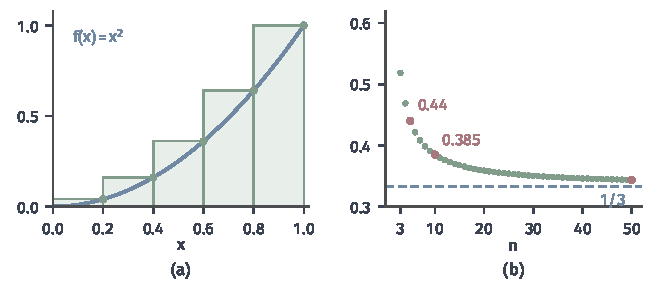
\includegraphics[width=112mm]{figures/07-probability/03-probability-limits/matplotlib/weak-lattice-uniform/figure.pdf}
 \caption{格点均匀分布的弱收敛。(a)$n=5$，浅绿柱宽$1/5$、高$f(k/5)$（绿点），面积之和为$\mathbb{E}[f(U_5)]=0.44$；蓝线为测试函数$f(x)=x^2$，其下面积为$1/3$。(b)$\mathbb{E}[f(U_n)]$随$n$的变化（绿点），蓝色虚线为极限$1/3$。}
 \label{fig:weak-lattice-uniform}
\end{BookInlineFigure}

\paragraph{极限的唯一性}
一列数的极限唯一。对分布也应如此，否则“极限分布”就不是一个确定的对象。这归结为：有界连续函数的读数能否区分两个分布。下面构造一族连续函数，从上方逼近闭集的示性函数。

对闭集$F\subset\mathbb{R}^{d}$，记点$\bm{x}$到$F$的距离为
\[
 \operatorname{dist}(\bm{x},F)=\inf_{\bm{y}\in F}\lVert\bm{x}-\bm{y}\rVert_2 ,
\]
并令
\begin{equation}
 f_k(\bm{x})=\max\bigl(0,\,1-k\operatorname{dist}(\bm{x},F)\bigr),\qquad k=1,2,\dots .
 \label{eq:weak-closed-approx}
\end{equation}
由三角不等式，距离函数满足
\[
 \lvert\operatorname{dist}(\bm{x},F)-\operatorname{dist}(\bm{y},F)\rvert\leq\lVert\bm{x}-\bm{y}\rVert_2 ,
\]
所以$f_k$连续，并且是Lipschitz常数为$k$的Lipschitz函数。它在$F$上等于$1$，在距$F$不小于$1/k$处等于$0$，取值在$[0,1]$中。

\begin{lemma}[有界连续函数确定分布]
\label{lem:weak-uniqueness}
设$P,Q$是$\mathbb{R}^{d}$上的概率分布。若对每个$f\in C_b(\mathbb{R}^{d})$都有$\int f\,\mathrm{d}P=\int f\,\mathrm{d}Q$，则$P=Q$。因此弱收敛的极限唯一：若$P_n\xrightarrow{\mathrm{w}}P$且$P_n\xrightarrow{\mathrm{w}}Q$，则$P=Q$。
\end{lemma}

\begin{proof}
取闭集$F$与式~\eqref{eq:weak-closed-approx}中的$f_k$。若$\bm{x}\in F$，则$f_k(\bm{x})=1$。若$\bm{x}\notin F$，因$F$闭，$\operatorname{dist}(\bm{x},F)>0$，当$k>1/\operatorname{dist}(\bm{x},F)$时$f_k(\bm{x})=0$。所以$f_k$逐点不增地趋于$\mathbf{1}_F$。

$0\leq f_k\leq1$，由支配收敛定理，
\[
 P(F)=\lim_{k\to\infty}\int f_k\,\mathrm{d}P=\lim_{k\to\infty}\int f_k\,\mathrm{d}Q=Q(F) .
\]
于是$P$与$Q$在全体闭集上相等。闭集族对有限交封闭，并且生成$\mathcal{B}(\mathbb{R}^{d})$。由第~\ref{chap:probability-spaces}章测度的唯一性定理，$P=Q$。

若$P_n$同时弱收敛到$P$和$Q$，则对每个$f\in C_b(\mathbb{R}^{d})$，$\int f\,\mathrm{d}P$与$\int f\,\mathrm{d}Q$是同一数列的极限，二者相等，再由前半部分得$P=Q$。
\end{proof}

\paragraph{同分布而样本不接近}
依分布收敛不涉及样本，下面的例子把这一点推到极端。取$\Omega=[0,1]$，$\mathbb{P}$为长度，令
\[
 X(\omega)=\omega,\qquad Y(\omega)=1-\omega .
\]
对$0\leq x\leq1$，$\mathbb{P}(Y\leq x)=\mathbb{P}(\omega\geq1-x)=x$，所以$X$与$Y$都服从$\operatorname{Unif}(0,1)$。令$X_n=Y$对一切$n$成立，则$X_n$与$X$的分布完全相同，$X_n\xrightarrow{\mathrm{d}}X$平凡地成立。

可是在样本点$\omega$上，$X_n$与$X$相差$\lvert1-2\omega\rvert$，与$n$无关，并且
\[
 \mathbb{P}\bigl(\lvert X_n-X\rvert>1/2\bigr)=\mathbb{P}\bigl(\omega<1/4\text{ 或 }\omega>3/4\bigr)=\frac12 .
\]
图~\ref{fig:weak-same-law}(a)画出这两个$\Omega$上的函数，它们在大部分样本点上相距很远；(b)是它们的直方图，完全一样。这好比两个班的身高分布相同，并不意味着按学号配对的两人身高接近。依分布收敛只比较“分布”这一侧，不管它由哪个函数实现。

\begin{BookInlineFigure}
 \centering
 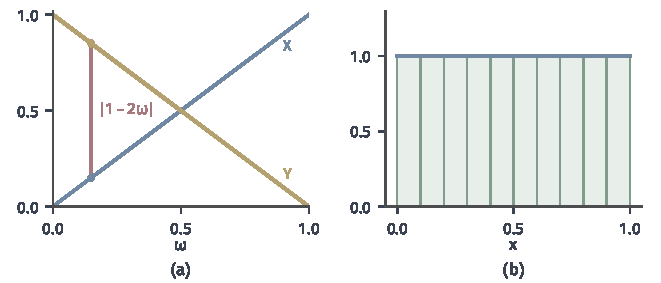
\includegraphics[width=112mm]{figures/07-probability/03-probability-limits/matplotlib/weak-same-law/figure.pdf}
 \caption{同分布而样本不接近。(a)$\Omega=[0,1]$上的$X(\omega)=\omega$（蓝）与$Y(\omega)=1-\omega$（黄），红色竖线段标出一个样本点上的差$\lvert1-2\omega\rvert$。(b)二者各用$\omega$的$2000$个等距点算出的直方图（浅绿），与$\operatorname{Unif}(0,1)$的密度（蓝）一致。}
 \label{fig:weak-same-law}
\end{BookInlineFigure}

\subsection{与依概率收敛的关系}
\label{sec:weak-probability-convergence}

当$\bm{X}_n$与$\bm{X}$定义在同一概率空间上时，第~\ref{chap:random-variable-convergence}章的依概率收敛$\bm{X}_n\xrightarrow{\mathbb{P}}\bm{X}$也有意义：对每个$\varepsilon>0$，事件$\lVert\bm{X}_n-\bm{X}\rVert_2\geq\varepsilon$的概率趋于零。上一个例子说明依分布收敛不能推出依概率收敛。反方向则成立：样本接近时，分布也接近。

\begin{theorem}[依概率收敛蕴含依分布收敛]
\label{thm:weak-prob-implies-dist}
设$\bm{X}_n$与$\bm{X}$是同一概率空间上取值于$\mathbb{R}^{d}$的随机向量。若$\bm{X}_n\xrightarrow{\mathbb{P}}\bm{X}$，则$\bm{X}_n\xrightarrow{\mathrm{d}}\bm{X}$。
\end{theorem}

\begin{proof}
取$f\in C_b(\mathbb{R}^{d})$，记$M=\sup\lvert f\rvert$，任取$\varepsilon>0$。困难在于$f$在整个空间上未必一致连续，所以先把$\bm{X}$限制在一个有界范围内。事件$\{\lVert\bm{X}\rVert_2>r\}$随$r$增大而下降到空集，由概率的连续性，存在$r$使$\mathbb{P}(\lVert\bm{X}\rVert_2>r)<\varepsilon$。

闭球$B=\{\lVert\bm{x}\rVert_2\leq r+1\}$是紧集，$f$在$B$上一致连续。于是存在$\delta\in(0,1)$，使得$\bm{x},\bm{y}\in B$且$\lVert\bm{x}-\bm{y}\rVert_2<\delta$时$\lvert f(\bm{x})-f(\bm{y})\rvert<\varepsilon$。

若$\lVert\bm{X}\rVert_2\leq r$且$\lVert\bm{X}_n-\bm{X}\rVert_2<\delta$，则$\bm{X}$与$\bm{X}_n$都在$B$中，$\lvert f(\bm{X}_n)-f(\bm{X})\rvert<\varepsilon$。其余情形用$\lvert f(\bm{X}_n)-f(\bm{X})\rvert\leq2M$。两部分合起来，
\[
 \bigl\lvert\mathbb{E}[f(\bm{X}_n)]-\mathbb{E}[f(\bm{X})]\bigr\rvert
 \leq\varepsilon+2M\,\mathbb{P}\bigl(\lVert\bm{X}\rVert_2>r\bigr)+2M\,\mathbb{P}\bigl(\lVert\bm{X}_n-\bm{X}\rVert_2\geq\delta\bigr) .
\]
令$n\to\infty$，最后一项趋于零，所以
\[
 \limsup_{n\to\infty}\bigl\lvert\mathbb{E}[f(\bm{X}_n)]-\mathbb{E}[f(\bm{X})]\bigr\rvert\leq\varepsilon+2M\varepsilon .
\]
$\varepsilon$任意，左边为零。
\end{proof}

反方向不成立，离散的例子更直接。设$X\sim\operatorname{Bern}(1/2)$，令$X_n=1-X$。$X_n$也服从$\operatorname{Bern}(1/2)$，所以$X_n\xrightarrow{\mathrm{d}}X$；但$\lvert X_n-X\rvert=1$恒成立，$\mathbb{P}(\lvert X_n-X\rvert\geq1/2)=1$。

\paragraph{极限为常量}
有一种情形反向结论成立：极限分布集中在一个点$\bm{c}$上。常量在任何概率空间上都可以定义，$\bm{X}_n\xrightarrow{\mathbb{P}}\bm{c}$只要求事件$\lVert\bm{X}_n-\bm{c}\rVert_2\geq\varepsilon$的概率趋于零，其中的概率在$\bm{X}_n$所在的空间上计算，所以即使各$\bm{X}_n$在不同的空间上，这个说法也有意义。

\begin{theorem}[依分布趋于常量]
\label{thm:weak-constant-limit}
设$\bm{c}\in\mathbb{R}^{d}$。若$\bm{X}_n\xrightarrow{\mathrm{d}}\bm{c}$，则对每个$\varepsilon>0$，
\begin{equation}
 \lim_{n\to\infty}\mathbb{P}\bigl(\lVert\bm{X}_n-\bm{c}\rVert_2\geq\varepsilon\bigr)=0 ,
 \label{eq:weak-constant-limit}
\end{equation}
即$\bm{X}_n\xrightarrow{\mathbb{P}}\bm{c}$。
\end{theorem}

\begin{proof}
令
\[
 h(\bm{x})=\min\bigl(1,\lVert\bm{x}-\bm{c}\rVert_2/\varepsilon\bigr) .
\]
它有界连续，$h(\bm{c})=0$，并且在$\lVert\bm{x}-\bm{c}\rVert_2\geq\varepsilon$处等于$1$，所以$h$处处不小于偏离事件$\{\lVert\bm{x}-\bm{c}\rVert_2\geq\varepsilon\}$的示性函数。取期望，
\[
 \mathbb{P}\bigl(\lVert\bm{X}_n-\bm{c}\rVert_2\geq\varepsilon\bigr)\leq\mathbb{E}\bigl[h(\bm{X}_n)\bigr]\longrightarrow h(\bm{c})=0 .
\]
\end{proof}

证明用一个连续函数从上方压住“偏离$\bm{c}$至少$\varepsilon$”的示性函数，见图~\ref{fig:weak-constant-limit}。常量之所以特殊，是因为它没有随机性需要与$\bm{X}_n$配对：知道$\bm{X}_n$的分布集中到$\bm{c}$附近，就知道$\bm{X}_n$本身以大概率在$\bm{c}$附近。第~\ref{sec:weak-slutsky}节的Slutsky定理要用到这一点。

\begin{BookInlineFigure}
 \centering
 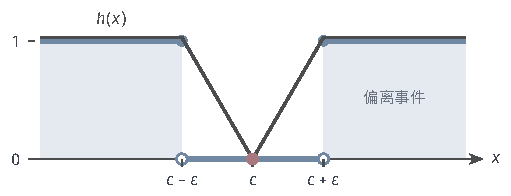
\includegraphics[width=86.6mm]{figures/07-probability/03-probability-limits/tikz/weak-constant-limit/figure.pdf}
 \caption{常量极限的证明。深灰折线为$h(x)=\min(1,\lvert x-c\rvert/\varepsilon)$，它连续且在$c$处为零；浅蓝区域为偏离事件$\{\lvert x-c\rvert\geq\varepsilon\}$，其示性函数（蓝色粗线）处处不超过$h$。}
 \label{fig:weak-constant-limit}
\end{BookInlineFigure}


\section{事件概率判据}
\label{sec:weak-event-criteria}

实际关心的往往是事件的概率：$X_n\leq x$的概率是否趋于$X\leq x$的概率，$\bm{X}_n$落在某个区域的概率是否收敛。事件的示性函数有界，却不连续，定义~\ref{def:weak-convergence}不能直接用于它。

两个例子说明困难确实存在。单点分布$\delta_{1/n}$趋于$\delta_0$，取$A=(0,\infty)$，则$\delta_{1/n}(A)=1$而$\delta_0(A)=0$；取$A=(-\infty,0]$，结果反过来。格点均匀分布$U_n\xrightarrow{\mathrm{d}}U\sim\operatorname{Unif}(0,1)$，取$A$为$[0,1]$中有理数的全体，则$\mathbb{P}(U_n\in A)=1$对一切$n$成立，而$\mathbb{P}(U\in A)=0$。

两个反例有共同的原因。记$\partial A$为$A$的边界，即闭包去掉内部。第一个例子中$\partial A=\{0\}$，极限分布在这里有质量$1$。第二个例子中，有理数的闭包是$[0,1]$，内部是空集，边界是整个$[0,1]$，极限分布在边界上的质量也是$1$。质量可以在极限过程中移到边界上，从$A$的一侧挪到另一侧，见图~\ref{fig:weak-boundary-mass}。本节证明：只有这种情形会出问题。

\begin{BookInlineFigure}
 \centering
 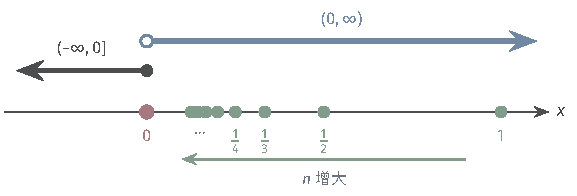
\includegraphics[width=97.6mm]{figures/07-probability/03-probability-limits/tikz/weak-boundary-mass/figure.pdf}
 \caption{质量移到边界上。绿点为$\delta_{1/n}$的质点位置$1,\,1/2,\,1/3,\dots$，红点为极限$\delta_0$的质点。蓝色为开集$(0,\infty)$，深灰为闭集$(-\infty,0]$，二者的公共边界是$0$：每个$\delta_{1/n}$都把全部质量放在开集里，极限却把它放在闭集里。}
 \label{fig:weak-boundary-mass}
\end{BookInlineFigure}

\subsection{Portmanteau定理}
\label{sec:weak-portmanteau}

图~\ref{fig:weak-boundary-mass}还显示了一个方向性：质量从开集一侧移到边界，闭集$(-\infty,0]$在极限中多得了质量，开集$(0,\infty)$在极限中失去了质量。一般地，极限过程中闭集的概率只能“突然增加”，开集的概率只能“突然减少”。用连续函数逼近示性函数，可以把这个直观变成不等式。

闭集$F$的示性函数由式~\eqref{eq:weak-closed-approx}的$f_k$从上方逼近。对开集$G$，补集$G^{\mathrm{c}}$闭，令
\begin{equation}
 g_k(\bm{x})=\min\bigl(1,\,k\operatorname{dist}(\bm{x},G^{\mathrm{c}})\bigr),\qquad k=1,2,\dots .
 \label{eq:weak-open-approx}
\end{equation}
$g_k$连续，取值在$[0,1]$中，在$G^{\mathrm{c}}$上为零，并且逐点不减地趋于$\mathbf{1}_G$：$\bm{x}\in G$时$\operatorname{dist}(\bm{x},G^{\mathrm{c}})>0$，$k$足够大后$g_k(\bm{x})=1$。图~\ref{fig:weak-portmanteau-approx}画出了区间上的这两族函数。

\begin{BookInlineFigure}
 \centering
 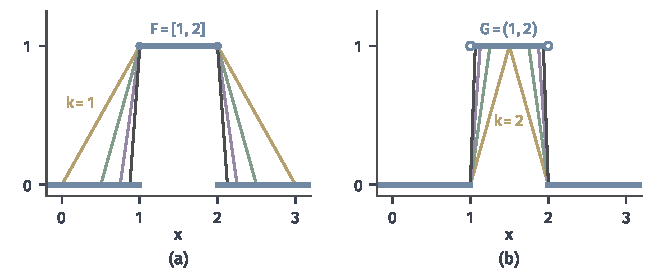
\includegraphics[width=112mm]{figures/07-probability/03-probability-limits/matplotlib/weak-portmanteau-approx/figure.pdf}
 \caption{用连续函数逼近示性函数。(a)闭区间$F=[1,2]$，$f_k$从上方逼近$\mathbf{1}_F$（蓝色粗线），黄、绿、紫、深灰依次为$k=1,2,4,8$。(b)开区间$G=(1,2)$，$g_k$从下方逼近$\mathbf{1}_G$，四种颜色依次为$k=2,4,8,16$。}
 \label{fig:weak-portmanteau-approx}
\end{BookInlineFigure}

\begin{theorem}[Portmanteau定理]
\label{thm:weak-portmanteau}
设$P_n$（$n\geq1$）与$P$是$\mathbb{R}^{d}$上的概率分布。以下五条等价：
\begin{enumerate}
 \item $P_n\xrightarrow{\mathrm{w}}P$；
 \item 对每个有界且Lipschitz连续的$f$，$\int f\,\mathrm{d}P_n\to\int f\,\mathrm{d}P$；
 \item 对每个闭集$F$，$\limsup_{n}P_n(F)\leq P(F)$；
 \item 对每个开集$G$，$\liminf_{n}P_n(G)\geq P(G)$；
 \item 对每个满足$P(\partial A)=0$的Borel集$A$，$P_n(A)\to P(A)$。
\end{enumerate}
\end{theorem}

\begin{proof}
(1)$\Rightarrow$(2)：有界Lipschitz函数是有界连续函数。

(2)$\Rightarrow$(3)：式~\eqref{eq:weak-closed-approx}的$f_k$有界且Lipschitz，并且$f_k\geq\mathbf{1}_F$。固定$k$，
\[
 \limsup_{n\to\infty}P_n(F)\leq\lim_{n\to\infty}\int f_k\,\mathrm{d}P_n=\int f_k\,\mathrm{d}P .
\]
引理~\ref{lem:weak-uniqueness}的证明已经说明$\int f_k\,\mathrm{d}P\to P(F)$。令$k\to\infty$即得(3)。

(3)$\Leftrightarrow$(4)：$G$为开集当且仅当$G^{\mathrm{c}}$为闭集，并且$P_n(G)=1-P_n(G^{\mathrm{c}})$，所以
\[
 \liminf_{n\to\infty}P_n(G)=1-\limsup_{n\to\infty}P_n(G^{\mathrm{c}})\geq1-P(G^{\mathrm{c}})=P(G) .
\]
反方向同理。

(3)与(4)$\Rightarrow$(5)：记$A^{\circ}$为$A$的内部，$\bar{A}$为闭包，则$A^{\circ}\subset A\subset\bar{A}$，且$\bar{A}\setminus A^{\circ}=\partial A$。由$P(\partial A)=0$得$P(A^{\circ})=P(A)=P(\bar{A})$。于是
\[
 \begin{aligned}
 \limsup_{n\to\infty}P_n(A)&\leq\limsup_{n\to\infty}P_n(\bar{A})\leq P(\bar{A})=P(A),\\
 \liminf_{n\to\infty}P_n(A)&\geq\liminf_{n\to\infty}P_n(A^{\circ})\geq P(A^{\circ})=P(A) .
 \end{aligned}
\]
上极限不超过下极限，所以$P_n(A)\to P(A)$。

(5)$\Rightarrow$(1)：取$f\in C_b(\mathbb{R}^{d})$。式~\eqref{eq:weak-definition}两边对$f$都是线性的，常数函数的读数恒为$1$，所以可以对$f$作正的伸缩与平移，不妨设$0<f<1$。由第~\ref{chap:tail-probabilities}章的尾积分公式，
\[
 \int f\,\mathrm{d}P=\int_0^1P(f>t)\,\mathrm{d}t ,
\]
对$P_n$同样成立。

集合$G_t=\{f>t\}$是开集，闭包含于$\{f\geq t\}$，所以$\partial G_t\subset\{f=t\}$。不同$t$对应的集合$\{f=t\}$互不相交，对每个正整数$m$，满足$P(f=t)\geq1/m$的$t$至多$m$个，所以$P(f=t)>0$的$t$至多可数。除去这些$t$，由(5)得$P_n(G_t)\to P(G_t)$。被积函数取值在$[0,1]$中，可数集长度为零，由支配收敛定理，
\[
 \int_0^1P_n(f>t)\,\mathrm{d}t\longrightarrow\int_0^1P(f>t)\,\mathrm{d}t ,
\]
即$\int f\,\mathrm{d}P_n\to\int f\,\mathrm{d}P$。
\end{proof}

\term{Portmanteau定理}（portmanteau theorem）的名字意为“手提箱”，指把几种等价说法装在一起。五条各有用途。(2)把测试函数缩小到有界Lipschitz函数，第~\ref{sec:weak-slutsky}节要用它。(3)和(4)说明极限中闭集可能多得质量、开集可能失去质量，图~\ref{fig:weak-boundary-mass}中两个不等号都是严格的：$\limsup\delta_{1/n}\bigl((-\infty,0]\bigr)=0<1$，$\liminf\delta_{1/n}\bigl((0,\infty)\bigr)=1>0$。(5)给出事件概率真正收敛的条件。

注意(5)中的条件只针对极限分布$P$，不针对$P_n$。格点均匀分布中，$A=[0,1/2]$的边界是$\{0,1/2\}$，$U_n$在$1/2$可能有质量（$n$为偶数时），但$\operatorname{Unif}(0,1)$在边界上没有质量，所以
\[
 \mathbb{P}(U_n\leq1/2)=\frac{\lfloor n/2\rfloor}{n}\longrightarrow\frac12 .
\]
$n=5$时为$0.4$，$n=11$时为$5/11\approx0.4545$，$n=101$时为$50/101\approx0.4950$。

边界有质量时，不能用示性函数代替连续测试函数。$\delta_{1/n}$与$A=(0,\infty)$就是这样：$P(\partial A)=\delta_0(\{0\})=1$，(5)的条件不满足，概率也确实不收敛。

\subsection{分布函数判据}
\label{sec:weak-cdf-criterion}

实轴上的分布由分布函数$F(x)=P\bigl((-\infty,x]\bigr)$确定。事件$(-\infty,x]$的边界是单点$\{x\}$，$P(\{x\})=0$恰好说明$F$在$x$处连续。于是Portmanteau定理的(5)直接给出：弱收敛时，分布函数在极限的连续点处收敛。下面的定理说明反过来也对。

\begin{theorem}[分布函数判据]
\label{thm:weak-cdf-criterion}
设$P_n$与$P$是$\mathbb{R}$上的概率分布，分布函数分别为$F_n$与$F$。则$P_n\xrightarrow{\mathrm{w}}P$，当且仅当
\begin{equation}
 \lim_{n\to\infty}F_n(x)=F(x)\qquad\text{对}F\text{的每个连续点}x .
 \label{eq:weak-cdf-criterion}
\end{equation}
\end{theorem}

\begin{proof}
必要性已由Portmanteau定理的(5)给出。下证充分性，验证(4)。

先说明$F$的连续点在$\mathbb{R}$中稠密。$F$的不连续点是$P$的原子，对每个正整数$m$，质量不小于$1/m$的原子至多$m$个，所以不连续点至多可数。可数集不含任何区间，因此每个区间中都有连续点。把连续点的全体记作$D$。

$\mathbb{R}$中的开集$G$是至多可数个互不相交的开区间之并，记作$G=\bigcup_jI_j$。任取$\varepsilon>0$。由可数可加性，可以取有限个$I_1,\dots,I_m$，使$\sum_{j\leq m}P(I_j)>P(G)-\varepsilon$。

设$I_j=(a_j,b_j)$，端点可以是$\pm\infty$。在$D$中取$a_j<a'_j<b'_j<b_j$，使$a'_j$充分接近$a_j$、$b'_j$充分接近$b_j$。由概率的连续性，可以做到
\[
 P\bigl((a'_j,b'_j]\bigr)>P(I_j)-\varepsilon/m .
\]

$(a'_j,b'_j]\subset I_j$，各$I_j$互不相交，所以
\[
 P_n(G)\geq\sum_{j=1}^{m}P_n\bigl((a'_j,b'_j]\bigr)=\sum_{j=1}^{m}\bigl(F_n(b'_j)-F_n(a'_j)\bigr) .
\]
右边是有限和，由式~\eqref{eq:weak-cdf-criterion}，它趋于
\[
 \sum_{j=1}^{m}\bigl(F(b'_j)-F(a'_j)\bigr)=\sum_{j=1}^{m}P\bigl((a'_j,b'_j]\bigr)>P(G)-2\varepsilon .
\]
于是$\liminf_nP_n(G)\geq P(G)-2\varepsilon$，$\varepsilon$任意，(4)成立。
\end{proof}

为什么必须排除跳点？$\delta_{1/n}$的分布函数是$F_n(x)=\mathbf{1}_{\{x\geq1/n\}}$，极限$\delta_0$的分布函数是$F(x)=\mathbf{1}_{\{x\geq0\}}$。逐点看：
\[
 \begin{aligned}
 &x<0: && F_n(x)=0=F(x);\\
 &x>0: && n>1/x\text{时}F_n(x)=1=F(x);\\
 &x=0: && F_n(0)=0\neq1=F(0) .
 \end{aligned}
\]
只有跳点$0$处不收敛。若质点从左边逼近，即$\delta_{-1/n}$，则$F_n(0)=1\to F(0)$。可见跳点处是否收敛取决于质量从哪一侧靠近，而弱收敛并不区分这两种靠近方式，图~\ref{fig:weak-cdf-criterion}(a)显示了这两种情形。

格点均匀分布的分布函数是阶梯$F_n(x)=\lfloor nx\rfloor/n$（$0\leq x\leq1$），极限$F(x)=x$处处连续。由$nx-1<\lfloor nx\rfloor\leq nx$，
\[
 \sup_{x\in\mathbb{R}}\lvert F_n(x)-F(x)\rvert\leq\frac1n .
\]
这里的收敛还是一致的，见图~\ref{fig:weak-cdf-criterion}(b)。

\begin{BookInlineFigure}
 \centering
 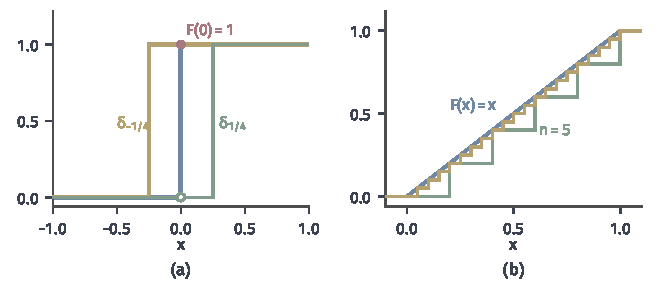
\includegraphics[width=112mm]{figures/07-probability/03-probability-limits/matplotlib/weak-cdf-criterion/figure.pdf}
 \caption{分布函数判据中的跳点。(a)蓝色为$\delta_0$的分布函数，绿色为$\delta_{1/4}$，黄色为$\delta_{-1/4}$；红点为$F(0)=1$，$\delta_{1/n}$在$0$处的值恒为$0$。(b)格点均匀分布$U_5$（绿色阶梯）与$U_{20}$（黄色阶梯）的分布函数，蓝线为$F(x)=x$。}
 \label{fig:weak-cdf-criterion}
\end{BookInlineFigure}

\paragraph{二项分布到Poisson分布}
现在可以把章首的现象写成定理。设$X_n\sim\operatorname{Bin}(n,2/n)$（$n\geq3$），$N\sim\operatorname{Poisson}(2)$。第~\ref{chap:common-distributions}章已经证明，对每个非负整数$k$，$\mathbb{P}(X_n=k)\to\mathbb{P}(N=k)$。分布函数在$x<0$时都为零；$x\geq0$时是有限和
\[
 F_n(x)=\sum_{k=0}^{\lfloor x\rfloor}\mathbb{P}(X_n=k)\longrightarrow\sum_{k=0}^{\lfloor x\rfloor}\mathbb{P}(N=k)=F(x) .
\]
所以$F_n(x)\to F(x)$对每个$x$成立，由定理~\ref{thm:weak-cdf-criterion}，$X_n\xrightarrow{\mathrm{d}}\operatorname{Poisson}(2)$。这里在跳点处也收敛；定理只是允许跳点处不收敛，并不要求它不收敛。

以$x=2$为例，$F(2)=5\mathrm{e}^{-2}\approx0.6767$，而
\[
 F_4(2)=0.6875,\qquad F_{10}(2)=0.6778,\qquad F_{40}(2)=0.6767 .
\]
图~\ref{fig:weak-binomial-poisson}(a)比较两个分布函数，(b)画出$\sup_x\lvert F_n(x)-F(x)\rvert$随$n$的变化，它大致按$1/n$缩小。弱收敛本身只断言极限，不给速度；这个速度是此例的具体计算结果。

\begin{BookInlineFigure}
 \centering
 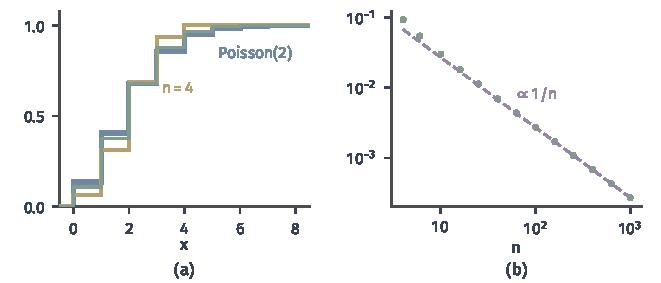
\includegraphics[width=112mm]{figures/07-probability/03-probability-limits/matplotlib/weak-binomial-poisson/figure.pdf}
 \caption{$\operatorname{Bin}(n,2/n)$向$\operatorname{Poisson}(2)$的弱收敛。(a)蓝色阶梯为$\operatorname{Poisson}(2)$的分布函数，黄色为$n=4$，绿色为$n=10$。(b)$\sup_x\lvert F_n(x)-F(x)\rvert$（绿点，对数坐标），紫色虚线是斜率为$-1$的参考线。}
 \label{fig:weak-binomial-poisson}
\end{BookInlineFigure}

分布函数判据还要求极限$F$本身是分布函数。若只知道$F_n$逐点收敛，极限可能不是分布函数：$\delta_n$的分布函数$\mathbf{1}_{\{x\geq n\}}$对每个$x$都趋于$0$。质量逃到了无穷远，下一节研究怎样防止这种情形。


\section{分布族的紧性}
\label{sec:weak-tightness}

前两节的判据都要先猜出极限分布，再去验证。很多时候极限并不知道，需要先判断一列分布有没有可能收敛到某个分布。实数列的情形可以作参照：有界数列不一定收敛，但总有收敛子列（Bolzano--Weierstrass定理）；无界数列可能连收敛子列都没有。分布列中扮演“无界”角色的，是概率质量逃向无穷远。

\paragraph{质量的逃逸}
$\delta_n$的全部质量跑到无穷远，分布函数对每个$x$都趋于$0$。逃逸也可以只是部分的。设$X_n\sim\mathcal{N}(0,n)$，则
\[
 F_n(x)=\Phi\bigl(x/\sqrt{n}\bigr)\longrightarrow\Phi(0)=\frac12,\qquad x\in\mathbb{R} .
\]
一半质量逃向$+\infty$，一半逃向$-\infty$，逐点极限是常数$1/2$，不是分布函数。再看$P_n=\frac12\delta_0+\frac12\delta_n$，它的分布函数趋于$\frac12\mathbf{1}_{\{x\geq0\}}$：留在原地的一半质量还在，跑远的一半消失了。图~\ref{fig:weak-mass-escape}画出这两种情形，它们都不可能弱收敛到任何概率分布。

\begin{BookInlineFigure}
 \centering
 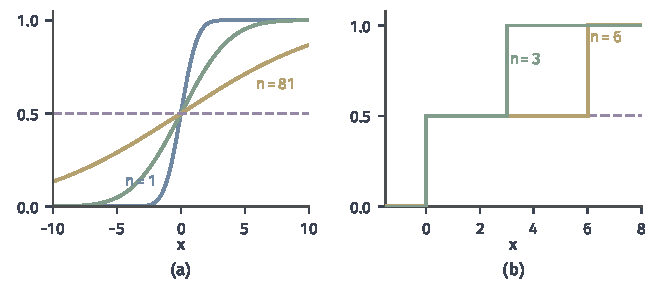
\includegraphics[width=112mm]{figures/07-probability/03-probability-limits/matplotlib/weak-mass-escape/figure.pdf}
 \caption{概率质量逃向无穷远。(a)$\mathcal{N}(0,n)$的分布函数，$n=1$（蓝）、$9$（绿）、$81$（黄），逐点趋于常数$1/2$（紫色虚线）。(b)$\frac12\delta_0+\frac12\delta_n$的分布函数，$n=3$（绿）与$n=6$（黄）；逐点极限$\frac12\mathbf{1}_{\{x\geq0\}}$（紫色虚线）的总质量只有$1/2$。}
 \label{fig:weak-mass-escape}
\end{BookInlineFigure}

\subsection{概率质量的控制}
\label{sec:weak-mass-control}

要防止逃逸，就要求所有分布在远处的质量能被同一个界控制。对单个分布这总能做到，因为$P(\lVert\bm{x}\rVert_2>r)$随$r\to\infty$趋于零；困难在于对一整族分布同时做到。

\begin{definition}[胎紧]
\label{def:weak-tight}
设$\{P_i\}_{i\in I}$是$\mathbb{R}^{d}$上的一族概率分布。若对每个$\varepsilon>0$，存在$r>0$使
\begin{equation}
 \sup_{i\in I}P_i\bigl(\{\bm{x}:\lVert\bm{x}\rVert_2>r\}\bigr)\leq\varepsilon ,
 \label{eq:weak-tight}
\end{equation}
则称这族分布\term{胎紧}（tight），也简称紧。一族随机向量称为胎紧，是指它们的分布胎紧。
\end{definition}

$\mathbb{R}^{d}$中有界闭集是紧集，所以式~\eqref{eq:weak-tight}也可以说成：存在紧集$K$，使每个$P_i$在$K$外的质量都不超过$\varepsilon$。单个分布胎紧；有限个胎紧族的并仍然胎紧，取各自的$r$中最大的一个即可。

直接验证式~\eqref{eq:weak-tight}往往不方便，矩的一致界给出常用的充分条件。

\begin{theorem}[矩的一致界蕴含胎紧]
\label{thm:weak-moment-tight}
设存在$p>0$与$M<\infty$，使$\mathbb{E}[\lVert\bm{X}_i\rVert_2^{p}]\leq M$对一切$i\in I$成立，则$\{\bm{X}_i\}_{i\in I}$胎紧，并且
\begin{equation}
 \sup_{i\in I}\mathbb{P}\bigl(\lVert\bm{X}_i\rVert_2>r\bigr)\leq\frac{M}{r^{p}},\qquad r>0 .
 \label{eq:weak-moment-tight}
\end{equation}
\end{theorem}

\begin{proof}
对非负变量$\lVert\bm{X}_i\rVert_2^{p}$用第~\ref{chap:tail-probabilities}章的Markov不等式，
\[
 \mathbb{P}\bigl(\lVert\bm{X}_i\rVert_2>r\bigr)\leq\mathbb{P}\bigl(\lVert\bm{X}_i\rVert_2^{p}\geq r^{p}\bigr)\leq\frac{M}{r^{p}} .
\]
取$r=(M/\varepsilon)^{1/p}$即得式~\eqref{eq:weak-tight}。
\end{proof}

对照前面的例子。$X_n\sim\operatorname{Bin}(n,2/n)$的期望恒为$2$，取$p=1$得$\mathbb{P}(X_n>r)\leq2/r$，胎紧。格点均匀分布都在$[0,1]$中，取$r=1$时式~\eqref{eq:weak-tight}左边为零。$\mathcal{N}(0,n)$的方差$n$没有一致界，它确实不胎紧：对任意固定的$r$，
\[
 \mathbb{P}(\lvert X_n\rvert>r)=2\bigl(1-\Phi(r/\sqrt{n})\bigr)\longrightarrow1 .
\]

\paragraph{胎紧与一致可积}
第~\ref{chap:random-variable-convergence}章的一致可积性也控制尾部，但控制的量不同。实随机变量族$\{X_i\}$一致可积，是指
\[
 \lim_{r\to\infty}\sup_{i\in I}\mathbb{E}\bigl[\lvert X_i\rvert\mathbf{1}_{\{\lvert X_i\rvert>r\}}\bigr]=0 .
\]
胎紧只数远处有多少质量；一致可积还要乘上质量所在的位置$\lvert x\rvert$，像力矩一样，远处的少量质量会被放大。在事件$\lvert X_i\rvert>r$上$\lvert X_i\rvert$至少是$r$，取期望得
\[
 \mathbb{P}\bigl(\lvert X_i\rvert>r\bigr)\leq\frac1r\,\mathbb{E}\bigl[\lvert X_i\rvert\mathbf{1}_{\{\lvert X_i\rvert>r\}}\bigr] ,
\]
所以一致可积蕴含胎紧。

反过来不成立。设$X_n$以概率$1/n$取$n$，以概率$1-1/n$取$0$。对$r\geq1$，只有$n>r$的那些$X_n$在$r$外有质量，质量为$1/n<1/r$，所以
\[
 \sup_{n}\mathbb{P}(X_n>r)\leq\frac1r,\qquad \sup_{n}\mathbb{E}\bigl[X_n\mathbf{1}_{\{X_n>r\}}\bigr]=\sup_{n>r}n\cdot\frac1n=1 .
\]
这族变量胎紧，却不一致可积。远处的质量$1/n$越来越少，而它与位置$n$的乘积始终是$1$。图~\ref{fig:weak-tight-vs-ui}对比了这两个量。第~\ref{sec:weak-integral-limits}节将看到，这个差别决定了期望能否随分布取极限。

\begin{BookInlineFigure}
 \centering
 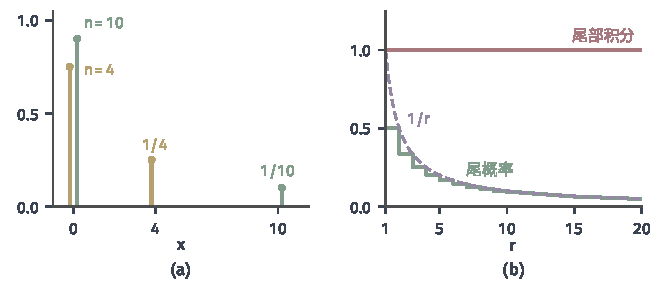
\includegraphics[width=112mm]{figures/07-probability/03-probability-limits/matplotlib/weak-tight-vs-ui/figure.pdf}
 \caption{胎紧与一致可积的差别，$X_n$以概率$1/n$取$n$，否则取$0$。(a)$n=4$（黄）与$n=10$（绿）的质量；远处质点很轻，乘以位置后都等于$1$。(b)作为$r$的函数，$\sup_n\mathbb{P}(X_n>r)$（绿）趋于零，紫色虚线为上界$1/r$；$\sup_n\mathbb{E}[X_n\mathbf{1}_{\{X_n>r\}}]$（红）恒为$1$。}
 \label{fig:weak-tight-vs-ui}
\end{BookInlineFigure}

\subsection{弱收敛子列}
\label{sec:weak-subsequences}

胎紧在分布列中的作用，正如有界性在实数列中的作用。下面的定理是Bolzano--Weierstrass定理的对应物。

\begin{theorem}[胎紧与弱收敛子列]
\label{thm:weak-prokhorov}
设$\{P_n\}$是$\mathbb{R}^{d}$上的概率分布列。
\begin{enumerate}
 \item 若$\{P_n\}$胎紧，则存在子列$P_{n_k}$与概率分布$P$，使$P_{n_k}\xrightarrow{\mathrm{w}}P$。
 \item 若一族分布中任取的序列都有弱收敛到概率分布的子列，则这族分布胎紧。
\end{enumerate}
\end{theorem}

后一条中的性质称为弱收敛意义下的相对紧。所以在$\mathbb{R}^{d}$中，胎紧与相对紧是同一回事。下面对$d=1$证明第一条，并对一般$d$证明第二条。

\begin{proof}
(1)，$d=1$。记$F_n$为$P_n$的分布函数，分四步。

第一步，用对角线方法在有理点上取收敛子列。把有理数排成$q_1,q_2,\dots$。数列$\bigl(F_n(q_1)\bigr)$在$[0,1]$中，有收敛子列；在这个子列中再取使$F_n(q_2)$收敛的子列，如此继续。取第$k$次所得子列的第$k$项，得到子列$(n_k)$，使对每个有理数$q$，$F_{n_k}(q)$收敛到某个$G(q)\in[0,1]$。$G$在有理数上不减。

第二步，构造右连续的极限。令
\[
 F(x)=\inf\{G(q):q\text{为有理数},\,q>x\} .
\]
$F$不减。若$x_m\downarrow x$，对每个有理数$q>x$，$m$足够大时$q>x_m$，于是$F(x_m)\leq G(q)$；对$q$取下确界得$\lim_mF(x_m)\leq F(x)$，而单调性给出反向不等式，所以$F$右连续。

第三步，在$F$的连续点$x$处证明$F_{n_k}(x)\to F(x)$。任取$\varepsilon>0$。由左连续性，取$y<x$使$F(y)>F(x)-\varepsilon$；由$F(x)$的定义，取有理数$s>x$使$G(s)<F(x)+\varepsilon$；再取有理数$r\in(y,x)$，由$F(y)$的定义有$F(y)\leq G(r)$。$F_{n_k}$不减，于是
\[
 \begin{aligned}
 \limsup_{k\to\infty}F_{n_k}(x)&\leq\lim_{k\to\infty}F_{n_k}(s)=G(s)<F(x)+\varepsilon,\\
 \liminf_{k\to\infty}F_{n_k}(x)&\geq\lim_{k\to\infty}F_{n_k}(r)=G(r)\geq F(y)>F(x)-\varepsilon .
 \end{aligned}
\]

第四步，用胎紧说明$F$是分布函数。对$\varepsilon>0$取式~\eqref{eq:weak-tight}中的$r$。对有理数$q>r$，$F_n(q)\geq1-\varepsilon$对一切$n$成立，所以$G(q)\geq1-\varepsilon$，从而$x\geq r$时$F(x)\geq1-\varepsilon$。对有理数$q<-r$，$F_n(q)\leq\varepsilon$，所以$x<q$时$F(x)\leq G(q)\leq\varepsilon$。因此$F(-\infty)=0$，$F(+\infty)=1$。不减、右连续且两端极限为$0$与$1$的函数是某个概率分布$P$的分布函数（第~\ref{chap:probability-spaces}章）。由定理~\ref{thm:weak-cdf-criterion}，$P_{n_k}\xrightarrow{\mathrm{w}}P$。

(2)，一般$d$。设这族分布不胎紧，则存在$\varepsilon>0$，对每个$m$都能在族中取到$P_m$，使$P_m(\lVert\bm{x}\rVert_2>m)>\varepsilon$。按假设，$(P_m)$有子列$P_{m_k}\xrightarrow{\mathrm{w}}P$。固定$r>0$，集合$\{\lVert\bm{x}\rVert_2\geq r\}$是闭集，当$m_k\geq r$时它包含$\{\lVert\bm{x}\rVert_2>m_k\}$。由Portmanteau定理的(3)，
\[
 P\bigl(\lVert\bm{x}\rVert_2\geq r\bigr)\geq\limsup_{k\to\infty}P_{m_k}\bigl(\lVert\bm{x}\rVert_2\geq r\bigr)\geq\varepsilon .
\]
这对每个$r$成立，与$P(\lVert\bm{x}\rVert_2\geq r)\to0$矛盾。
\end{proof}

第一步取出的极限$G$总存在，第四步之前的$F$也总能构造出来，胎紧只在第四步起作用。图~\ref{fig:weak-mass-escape}(b)就是缺了第四步的情形：前三步的构造给出$\frac12\mathbf{1}_{\{x\geq0\}}$，它右连续、不减，但$F(+\infty)=1/2$。$d>1$时第一条的证明思路相同，用多元分布函数在有理点上取对角线子列，细节较繁，可查阅~\scite{math-kallenberg2021probability}。

定理的第一条也称为\term{Helly选择定理}（Helly selection theorem）。在一般的完备可分度量空间上，胎紧（式~\eqref{eq:weak-tight}中的球换成紧集）与相对紧仍然等价，这就是\term{Prokhorov定理}（Prokhorov theorem）；空间的完备与可分保证单个分布胎紧，是相对紧推出胎紧所需的条件。本卷只在有限维空间中使用它。

\paragraph{子列极限的唯一性}
胎紧只保证有收敛子列，不保证整列收敛。$P_n$在$\delta_0$与$\delta_1$之间交替，所有质量都在$[0,1]$中，胎紧；偶数项与奇数项各自收敛，极限不同，整列不收敛。数列的情形也一样：有界数列收敛，当且仅当它所有收敛子列的极限相同。

\begin{lemma}[子列原则]
\label{lem:weak-subsequence}
设$\{P_n\}$胎紧，并且每个弱收敛的子列都收敛到同一个分布$P$，则$P_n\xrightarrow{\mathrm{w}}P$。
\end{lemma}

\begin{proof}
若不然，存在$f\in C_b(\mathbb{R}^{d})$、$\varepsilon>0$和子列$(n_k)$，使对一切$k$，
\[
 \Bigl\lvert\int f\,\mathrm{d}P_{n_k}-\int f\,\mathrm{d}P\Bigr\rvert\geq\varepsilon .
\]
子列仍胎紧，由定理~\ref{thm:weak-prokhorov}，它有进一步的子列弱收敛，按假设极限为$P$。沿这个进一步的子列，$\int f\,\mathrm{d}P_{n_k}\to\int f\,\mathrm{d}P$，与上式矛盾。
\end{proof}

这个引理把弱收敛的证明分成两件互相独立的事：用胎紧得到子列极限的存在，用别的办法证明子列极限只有一个。第~\ref{sec:weak-cf}节将用特征函数完成后一件事。


\section{特征函数}
\label{sec:weak-cf}

按定义验证弱收敛，要对每个有界连续函数检查读数，这在实际中无法做到。我们希望找一小族测试函数，它们由一个参数标记，同时满足三点：读数能确定分布；读数的收敛能推出弱收敛；独立变量相加时读数容易计算。复指数$\mathrm{e}^{\mathrm{i}tx}$正好满足这些要求。它的实部$\cos(tx)$与虚部$\sin(tx)$都有界连续；并且
\[
 \mathrm{e}^{\mathrm{i}t(x+y)}=\mathrm{e}^{\mathrm{i}tx}\,\mathrm{e}^{\mathrm{i}ty} ,
\]
加法变成了乘法。本节依次建立它的定义、运算、与矩的关系、对分布的识别，以及与弱收敛的联系。所需的Fourier分析都在概率对象上直接说明，不假定分布有密度。

\subsection{定义}
\label{sec:weak-cf-definition}

复值随机变量$Y_1+\mathrm{i}Y_2$的期望按实部、虚部分别取：
\[
 \mathbb{E}[Y_1+\mathrm{i}Y_2]=\mathbb{E}[Y_1]+\mathrm{i}\,\mathbb{E}[Y_2] .
\]
复值积分的性质可参考\BookChapterRef{chap:integration}{卷四第6章“积分”}，这里要用的是线性，以及期望的模不超过模的期望。

\begin{definition}[特征函数]
\label{def:weak-cf}
实随机变量$X$的\term{特征函数}（characteristic function）是
\begin{equation}
 \phi_X(t)=\mathbb{E}\bigl[\mathrm{e}^{\mathrm{i}tX}\bigr]=\mathbb{E}[\cos(tX)]+\mathrm{i}\,\mathbb{E}[\sin(tX)],\qquad t\in\mathbb{R} .
 \label{eq:weak-cf}
\end{equation}
取值于$\mathbb{R}^{d}$的随机向量$\bm{X}$的特征函数是
\begin{equation}
 \phi_{\bm{X}}(\bm{t})=\mathbb{E}\bigl[\mathrm{e}^{\mathrm{i}\langle\bm{t},\bm{X}\rangle}\bigr],\qquad \bm{t}\in\mathbb{R}^{d} .
 \label{eq:weak-cf-vector}
\end{equation}
\end{definition}

$\lvert\cos(tX)\rvert$与$\lvert\sin(tX)\rvert$都不超过$1$，所以特征函数对每个随机变量、每个$t$都存在，不需要任何矩条件。它只依赖$X$的分布，对分布$P$也写作$\phi_P$。

\paragraph{单位圆上的重心}
$\mathrm{e}^{\mathrm{i}tx}$是单位圆上辐角为$tx$的点。固定频率$t$，把取值$x$处的质量搬到单位圆上这个点，$\phi_X(t)$就是搬过去以后的重心。$t$很小时，各点挤在$1$附近，重心接近$1$；$t$变大，各点沿圆周散开，彼此抵消，重心向原点靠拢。所以$\lvert\phi_X(t)\rvert$描述分布在频率$t$下“转散”以后还剩多少一致性。

以均匀骰子为例，$X$在$\{1,\dots,6\}$上等可能取值，
\[
 \phi_X(t)=\frac16\sum_{k=1}^{6}\mathrm{e}^{\mathrm{i}tk} .
\]
$t=0.5$时，六个点散布在辐角$0.5$到$3$之间，重心约为$-0.120+0.661\mathrm{i}$，模约$0.672$。$t=\pi/3$时，六个点恰是正六边形的顶点，重心为$0$。图~\ref{fig:weak-cf-circle}画出这两个频率下的点与重心。

\begin{BookInlineFigure}
 \centering
 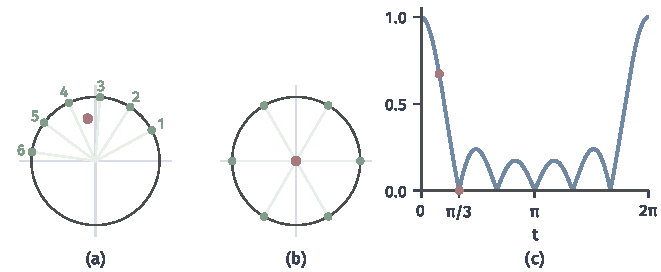
\includegraphics[width=112mm]{figures/07-probability/03-probability-limits/matplotlib/weak-cf-circle/figure.pdf}
 \caption{特征函数是单位圆上的重心。$X$为均匀骰子点数，绿点为$\mathrm{e}^{\mathrm{i}tk}$（$k=1,\dots,6$），每点质量$1/6$，红点为重心$\phi_X(t)$。(a)$t=0.5$；(b)$t=\pi/3$，六点构成正六边形，重心为$0$。(c)$\lvert\phi_X(t)\rvert$，$0\leq t\leq2\pi$，红点对应(a)(b)两个频率。}
 \label{fig:weak-cf-circle}
\end{BookInlineFigure}

\paragraph{基本性质}
由定义直接得到三条性质。第一，$\phi_X(0)=1$，且
\[
 \lvert\phi_X(t)\rvert\leq\mathbb{E}\bigl[\lvert\mathrm{e}^{\mathrm{i}tX}\rvert\bigr]=1 .
\]
第二，共轭对称：$\mathrm{e}^{-\mathrm{i}tX}$是$\mathrm{e}^{\mathrm{i}tX}$的共轭，所以$\phi_X(-t)=\overline{\phi_X(t)}$。若$X$与$-X$同分布，则$\phi_X(t)=\phi_{-X}(t)=\phi_X(-t)$，再由共轭对称，$\phi_X(t)$等于自己的共轭，特征函数是实的。

第三，一致连续。对任意$t$与$h$，
\[
 \lvert\phi_X(t+h)-\phi_X(t)\rvert=\bigl\lvert\mathbb{E}\bigl[\mathrm{e}^{\mathrm{i}tX}(\mathrm{e}^{\mathrm{i}hX}-1)\bigr]\bigr\rvert\leq\mathbb{E}\bigl[\lvert\mathrm{e}^{\mathrm{i}hX}-1\rvert\bigr] .
\]
右边不含$t$。$h\to0$时$\lvert\mathrm{e}^{\mathrm{i}hX}-1\rvert$逐点趋于零且不超过$2$，由支配收敛定理，右边趋于零。随机向量的情形完全相同。

\paragraph{常见分布}
离散分布按定义求和。$X\sim\operatorname{Bern}(p)$时，$\phi_X(t)=1-p+p\,\mathrm{e}^{\mathrm{i}t}$。$N\sim\operatorname{Poisson}(\lambda)$时，用指数函数的幂级数，
\[
 \phi_N(t)=\sum_{k\geq0}\mathrm{e}^{-\lambda}\frac{(\lambda\mathrm{e}^{\mathrm{i}t})^{k}}{k!}=\exp\bigl(\lambda(\mathrm{e}^{\mathrm{i}t}-1)\bigr) .
\]

有密度的分布按定义积分。$X\sim\operatorname{Unif}(-1,1)$时，虚部的被积函数是奇函数，积分为零，
\[
 \phi_X(t)=\frac12\int_{-1}^{1}\cos(tx)\,\mathrm{d}x=\frac{\sin t}{t},\qquad t\neq0 ,
\]
$\phi_X(0)=1$。

标准高斯$Z\sim\mathcal{N}(0,1)$的特征函数用一个微分方程求出。先说明可以在积分号下对$t$求导。对实数$a$，
\[
 \lvert\mathrm{e}^{\mathrm{i}a}-1\rvert=\Bigl\lvert\int_0^a\mathrm{i}\,\mathrm{e}^{\mathrm{i}s}\,\mathrm{d}s\Bigr\rvert\leq\lvert a\rvert .
\]
于是差商满足
\[
 \Bigl\lvert\mathrm{e}^{\mathrm{i}tx}\,\frac{\mathrm{e}^{\mathrm{i}hx}-1}{h}\,\varphi(x)\Bigr\rvert\leq\lvert x\rvert\varphi(x) .
\]
右边可积，由支配收敛定理，
\[
 \phi_Z'(t)=\int_{-\infty}^{\infty}\mathrm{i}x\,\mathrm{e}^{\mathrm{i}tx}\varphi(x)\,\mathrm{d}x .
\]

再用$x\varphi(x)=-\varphi'(x)$分部积分。边界项$\mathrm{e}^{\mathrm{i}tx}\varphi(x)$在$\pm\infty$处为零，于是
\[
 \phi_Z'(t)=-\mathrm{i}\int_{-\infty}^{\infty}\mathrm{e}^{\mathrm{i}tx}\varphi'(x)\,\mathrm{d}x=\mathrm{i}\int_{-\infty}^{\infty}\mathrm{i}t\,\mathrm{e}^{\mathrm{i}tx}\varphi(x)\,\mathrm{d}x=-t\,\phi_Z(t) .
\]
由此$\bigl(\mathrm{e}^{t^2/2}\phi_Z(t)\bigr)'=0$，结合$\phi_Z(0)=1$，得
\begin{equation}
 \phi_Z(t)=\mathrm{e}^{-t^2/2} .
 \label{eq:weak-gaussian-cf}
\end{equation}
标准高斯的特征函数与密度只差一个常数因子，这是后面高斯平滑论证的关键。

\subsection{变换与独立和}
\label{sec:weak-cf-operations}

先看确定的线性变换。对实数$a,b$，把$\mathrm{e}^{\mathrm{i}t(aX+b)}$拆成$\mathrm{e}^{\mathrm{i}tb}$与$\mathrm{e}^{\mathrm{i}(at)X}$之积，取期望得
\begin{equation}
 \phi_{aX+b}(t)=\mathrm{e}^{\mathrm{i}tb}\,\phi_X(at) .
 \label{eq:weak-cf-affine}
\end{equation}
平移只乘一个模为一的因子，不改变$\lvert\phi\rvert$；数乘$a$把频率轴伸缩$a$倍。对随机向量，设$\bm{A}$是$k\times d$矩阵，$\bm{b}\in\mathbb{R}^{k}$。由
\[
 \langle\bm{t},\bm{A}\bm{X}\rangle=\langle\bm{A}^{\top}\bm{t},\bm{X}\rangle ,
\]
得到
\begin{equation}
 \phi_{\bm{A}\bm{X}+\bm{b}}(\bm{t})=\mathrm{e}^{\mathrm{i}\langle\bm{t},\bm{b}\rangle}\,\phi_{\bm{X}}(\bm{A}^{\top}\bm{t}),\qquad\bm{t}\in\mathbb{R}^{k} .
 \label{eq:weak-cf-linear}
\end{equation}

例如$X\sim\mathcal{N}(\mu,\sigma^2)$可以写成$\mu+\sigma Z$，由式~\eqref{eq:weak-gaussian-cf}与式~\eqref{eq:weak-cf-affine}，
\[
 \phi_X(t)=\exp\Bigl(\mathrm{i}\mu t-\frac{\sigma^2t^2}{2}\Bigr) .
\]

\paragraph{独立和}
独立性把乘积的期望拆成期望的乘积，这正是复指数的加法性质需要的。

\begin{theorem}[独立和的特征函数]
\label{thm:weak-cf-independent}
设$\bm{X}$与$\bm{Y}$是相互独立、分别取值于$\mathbb{R}^{d}$与$\mathbb{R}^{k}$的随机向量。则联合特征函数可以分解为
\begin{equation}
 \phi_{(\bm{X},\bm{Y})}(\bm{s},\bm{t})=\phi_{\bm{X}}(\bm{s})\,\phi_{\bm{Y}}(\bm{t}),\qquad\bm{s}\in\mathbb{R}^{d},\ \bm{t}\in\mathbb{R}^{k} .
 \label{eq:weak-cf-joint-independent}
\end{equation}
特别地，$k=d$时，
\begin{equation}
 \phi_{\bm{X}+\bm{Y}}(\bm{t})=\phi_{\bm{X}}(\bm{t})\,\phi_{\bm{Y}}(\bm{t}) .
 \label{eq:weak-cf-sum}
\end{equation}
对相互独立的$\bm{X}_1,\dots,\bm{X}_n$，和的特征函数是$\prod_{j}\phi_{\bm{X}_j}$。
\end{theorem}

\begin{proof}
对有界可测的实函数$g,h$，独立性给出（第~\ref{chap:random-vectors}章）
\[
 \mathbb{E}[g(\bm{X})h(\bm{Y})]=\mathbb{E}[g(\bm{X})]\,\mathbb{E}[h(\bm{Y})] .
\]
把$\mathrm{e}^{\mathrm{i}\langle\bm{s},\bm{X}\rangle}$与$\mathrm{e}^{\mathrm{i}\langle\bm{t},\bm{Y}\rangle}$各自拆成实部与虚部，它们都是有界可测函数，乘开后有四项，每项都按上式分解，再合并，即得式~\eqref{eq:weak-cf-joint-independent}。取$\bm{s}=\bm{t}$，由内积的线性得式~\eqref{eq:weak-cf-sum}。$n$项的情形对$n$归纳。
\end{proof}

用已知分布检验这个公式。$\operatorname{Bin}(n,p)$是$n$个独立$\operatorname{Bern}(p)$之和，按式~\eqref{eq:weak-cf-sum}，
\[
 \phi(t)=\bigl(1-p+p\,\mathrm{e}^{\mathrm{i}t}\bigr)^{n} .
\]
按定义直接求和，由二项式定理，
\[
 \sum_{k=0}^{n}\binom nkp^{k}(1-p)^{n-k}\mathrm{e}^{\mathrm{i}tk}=\bigl(1-p+p\,\mathrm{e}^{\mathrm{i}t}\bigr)^{n} ,
\]
两者一致。独立的$\operatorname{Poisson}(\lambda_1)$与$\operatorname{Poisson}(\lambda_2)$之和，特征函数是$\exp\bigl((\lambda_1+\lambda_2)(\mathrm{e}^{\mathrm{i}t}-1)\bigr)$，正是$\operatorname{Poisson}(\lambda_1+\lambda_2)$的特征函数；下一小节的唯一性定理说明，和就服从这个分布。

多元高斯也可以这样算。设$\bm{Z}=(Z_1,\dots,Z_m)$的分量是独立的标准高斯变量，由式~\eqref{eq:weak-cf-joint-independent}，
\[
 \phi_{\bm{Z}}(\bm{s})=\prod_{j=1}^{m}\mathrm{e}^{-s_j^2/2}=\mathrm{e}^{-\lVert\bm{s}\rVert_2^2/2} .
\]
第~\ref{chap:multivariate-distributions}章把与$\bm{\mu}+\bm{A}\bm{Z}$同分布的随机向量$\bm{X}$定义为服从$\mathcal{N}(\bm{\mu},\bm{\Sigma})$，其中$\bm{\Sigma}=\bm{A}\bm{A}^{\top}$。由式~\eqref{eq:weak-cf-linear}，
\begin{equation}
 \phi_{\bm{X}}(\bm{t})=\exp\Bigl(\mathrm{i}\langle\bm{t},\bm{\mu}\rangle-\frac12\lVert\bm{A}^{\top}\bm{t}\rVert_2^2\Bigr)=\exp\Bigl(\mathrm{i}\langle\bm{t},\bm{\mu}\rangle-\frac12\bm{t}^{\top}\bm{\Sigma}\bm{t}\Bigr) .
 \label{eq:weak-mvn-cf}
\end{equation}
结果只通过$\bm{\Sigma}$依赖$\bm{A}$，与那一章的结论一致；$\bm{\Sigma}$奇异时公式照样成立。

\paragraph{没有独立时}
式~\eqref{eq:weak-cf-sum}离不开独立性。设$X\sim\operatorname{Unif}(-1,1)$，若$Y$是与$X$独立的同分布变量，$X+Y$的密度是$[-2,2]$上的三角形（第~\ref{chap:random-variable-transformations}章的卷积），特征函数是$(\sin t/t)^2$。若取$Y=X$，和是$2X$，由式~\eqref{eq:weak-cf-affine}，特征函数是$\sin(2t)/(2t)$。在$t=\pi/2$处，
\[
 \frac{\sin\pi}{\pi}=0,\qquad\Bigl(\frac{\sin(\pi/2)}{\pi/2}\Bigr)^{2}=\frac{4}{\pi^{2}}\approx0.405 ,
\]
两者不同。图~\ref{fig:weak-cf-sum}把两种和的密度与特征函数并排画出：边缘相同，配对方式不同，和的分布就不同。

\begin{BookInlineFigure}
 \centering
 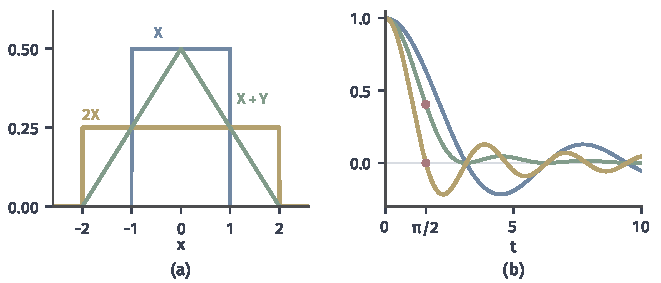
\includegraphics[width=112mm]{figures/07-probability/03-probability-limits/matplotlib/weak-cf-sum/figure.pdf}
 \caption{独立和与非独立和。(a)$\operatorname{Unif}(-1,1)$的密度（蓝），两个独立副本之和的三角形密度（绿），$2X$的均匀密度（黄）。(b)对应的特征函数$\sin t/t$、$(\sin t/t)^2$与$\sin(2t)/(2t)$，红点标出$t=\pi/2$处的两个值$4/\pi^2$与$0$。}
 \label{fig:weak-cf-sum}
\end{BookInlineFigure}

\subsection{矩与局部展开}
\label{sec:weak-cf-moments}

特征函数在原点附近的形状记录了矩。$\mathrm{e}^{\mathrm{i}tx}$对$t$求一次导数多出因子$\mathrm{i}x$，所以对期望求导，若能与期望交换，就得到$\mathbb{E}[\mathrm{i}X\mathrm{e}^{\mathrm{i}tX}]$。交换的条件是相应的绝对矩有限。为了控制余项，先给出复指数Taylor展开的误差界。

\begin{lemma}[复指数的展开误差]
\label{lem:weak-exp-remainder}
对实数$x$与整数$m\geq0$，
\begin{equation}
 \Bigl\lvert\mathrm{e}^{\mathrm{i}x}-\sum_{j=0}^{m}\frac{(\mathrm{i}x)^{j}}{j!}\Bigr\rvert\leq\min\Bigl(\frac{\lvert x\rvert^{m+1}}{(m+1)!},\ \frac{2\lvert x\rvert^{m}}{m!}\Bigr) .
 \label{eq:weak-exp-remainder}
\end{equation}
\end{lemma}

\begin{proof}
记左边绝对值内的量为$R_m(x)$。对$x$求导，
\[
 R_m'(x)=\mathrm{i}\,\mathrm{e}^{\mathrm{i}x}-\sum_{j=1}^{m}\frac{\mathrm{i}(\mathrm{i}x)^{j-1}}{(j-1)!}=\mathrm{i}R_{m-1}(x) ,
\]
又$R_m(0)=0$，所以$R_m(x)=\mathrm{i}\int_0^xR_{m-1}(s)\,\mathrm{d}s$。

对$m$归纳。$m=0$时，$R_0(x)=\mathrm{e}^{\mathrm{i}x}-1$，前面计算高斯特征函数时已经说明它的模不超过$\lvert x\rvert$；又由三角不等式，$\lvert R_0(x)\rvert\leq2$。设结论对$m-1$成立，则
\[
 \lvert R_m(x)\rvert\leq\int_0^{\lvert x\rvert}\min\Bigl(\frac{s^{m}}{m!},\frac{2s^{m-1}}{(m-1)!}\Bigr)\mathrm{d}s .
\]
分别只用最小值中的一项积分，得到$\lvert x\rvert^{m+1}/(m+1)!$与$2\lvert x\rvert^{m}/m!$两个上界。
\end{proof}

两个上界各有用处：$\lvert x\rvert$小时第一个更小，$\lvert x\rvert$大时第二个只增长到$m$次幂。下面的论证会同时用到这两种情形。

\begin{theorem}[矩与导数]
\label{thm:weak-cf-derivatives}
设$k\geq1$为整数，$\mathbb{E}[\lvert X\rvert^{k}]<\infty$。则$\phi_X$有直到$k$阶的连续导数，
\begin{equation}
 \phi_X^{(j)}(t)=\mathbb{E}\bigl[(\mathrm{i}X)^{j}\mathrm{e}^{\mathrm{i}tX}\bigr],\qquad
 \phi_X^{(j)}(0)=\mathrm{i}^{j}\,\mathbb{E}[X^{j}],\qquad j=0,1,\dots,k .
 \label{eq:weak-cf-derivatives}
\end{equation}
\end{theorem}

\begin{proof}
对$j$归纳，$j=0$即定义。设$j<k$时公式成立，考虑差商
\[
 \frac{\phi_X^{(j)}(t+h)-\phi_X^{(j)}(t)}{h}=\mathbb{E}\Bigl[(\mathrm{i}X)^{j}\mathrm{e}^{\mathrm{i}tX}\,\frac{\mathrm{e}^{\mathrm{i}hX}-1}{h}\Bigr] .
\]
由引理~\ref{lem:weak-exp-remainder}（$m=0$），期望内的量的模不超过$\lvert X\rvert^{j+1}$。$j+1\leq k$，且$\lvert X\rvert^{j+1}\leq1+\lvert X\rvert^{k}$，所以它可积。$h\to0$时期望内的量逐点趋于$(\mathrm{i}X)^{j+1}\mathrm{e}^{\mathrm{i}tX}$，由支配收敛定理得到$j+1$阶的公式。导数的连续性同样由支配收敛定理得到，控制函数是$\lvert X\rvert^{j}$。取$t=0$即得原点处的值。
\end{proof}

例如$N\sim\operatorname{Poisson}(2)$，它的特征函数已在第~\ref{sec:weak-cf-definition}节求出。逐次求导，
\[
 \begin{aligned}
 \phi_N'(t)&=2\mathrm{i}\,\mathrm{e}^{\mathrm{i}t}\phi_N(t),\\
 \phi_N''(t)&=\bigl((2\mathrm{i}\,\mathrm{e}^{\mathrm{i}t})^{2}-2\,\mathrm{e}^{\mathrm{i}t}\bigr)\phi_N(t) .
 \end{aligned}
\]
在原点，$\phi_N'(0)=2\mathrm{i}$，$\phi_N''(0)=-4-2=-6$。由式~\eqref{eq:weak-cf-derivatives}，
\[
 \mathbb{E}[N]=2,\qquad\mathbb{E}[N^{2}]=6,\qquad\operatorname{Var}(N)=6-4=2 ,
\]
与第~\ref{chap:common-distributions}章的结果相同。这里先由Poisson分布的各阶矩有限（其尾部比任何幂次都轻）保证求导合法，再读出矩。

\paragraph{二阶展开}
中心极限定理只需要原点附近到二阶的展开，而且只假定二阶矩有限。下面的定理给出展开和余项的控制。

\begin{theorem}[特征函数的二阶展开]
\label{thm:weak-cf-second-order}
设$\mathbb{E}[X^{2}]<\infty$。则
\begin{equation}
 \begin{gathered}
 \phi_X(t)=1+\mathrm{i}t\,\mathbb{E}[X]-\frac{t^{2}}{2}\mathbb{E}[X^{2}]+r(t),\\
 \lvert r(t)\rvert\leq t^{2}\,\mathbb{E}\Bigl[\min\Bigl(\frac{\lvert t\rvert\lvert X\rvert^{3}}{6},\,X^{2}\Bigr)\Bigr] ,
 \end{gathered}
 \label{eq:weak-cf-second-order}
\end{equation}
并且$r(t)/t^{2}\to0$（$t\to0$）。特别地，若$\mathbb{E}[X]=0$，$\operatorname{Var}(X)=\sigma^{2}$，则$\phi_X(t)=1-\sigma^{2}t^{2}/2+r(t)$。
\end{theorem}

\begin{proof}
在引理~\ref{lem:weak-exp-remainder}中取$m=2$，$x=tX$，
\[
 \Bigl\lvert\mathrm{e}^{\mathrm{i}tX}-1-\mathrm{i}tX+\frac{t^{2}X^{2}}{2}\Bigr\rvert\leq\min\Bigl(\frac{\lvert tX\rvert^{3}}{6},\,\lvert tX\rvert^{2}\Bigr)=t^{2}\min\Bigl(\frac{\lvert t\rvert\lvert X\rvert^{3}}{6},\,X^{2}\Bigr) .
\]
取期望，左边期望的模不小于$\lvert r(t)\rvert$，得到式~\eqref{eq:weak-cf-second-order}中的余项界。

$t\to0$时，对每个样本点，余项界中期望内的量不超过$\lvert t\rvert\lvert X\rvert^{3}/6$，因而趋于零；它又被可积的$X^{2}$控制。由支配收敛定理，余项界中的期望趋于零，即$r(t)/t^{2}\to0$。
\end{proof}

这里同时用了引理的两个上界。若只用$\lvert tX\rvert^{3}/6$，就需要三阶矩有限；$X^{2}$这一项让定理只依赖二阶矩，代价是只知道$r(t)=o(t^{2})$，不知道它以什么速度趋于零。

图~\ref{fig:weak-cf-local}比较三个均值为$0$、方差为$1$的分布：以$\pm1$各半取值的变量，特征函数为$\cos t$；$\operatorname{Unif}(-\sqrt3,\sqrt3)$，特征函数为$\sin(\sqrt3t)/(\sqrt3t)$；标准高斯$\mathrm{e}^{-t^{2}/2}$。三条曲线在原点附近都贴着抛物线$1-t^{2}/2$，离开原点后才分开。它们的四阶Taylor系数分别是$1/24$、$3/40$与$1/8$，正是四阶矩除以$4!$的不同。

\begin{BookInlineFigure}
 \centering
 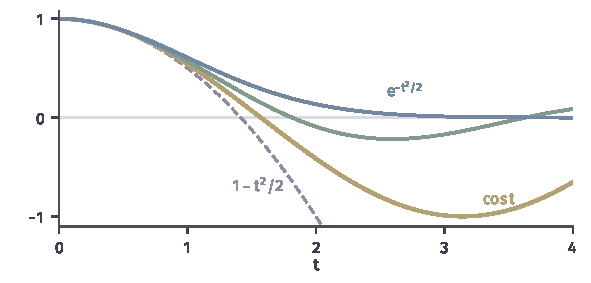
\includegraphics[width=100mm]{figures/07-probability/03-probability-limits/matplotlib/weak-cf-local/figure.pdf}
 \caption{特征函数的二阶展开。均值为$0$、方差为$1$的三个分布：$\pm1$各半（黄，$\cos t$），$\operatorname{Unif}(-\sqrt3,\sqrt3)$（绿），$\mathcal{N}(0,1)$（蓝）；紫色虚线为抛物线$1-t^{2}/2$。}
 \label{fig:weak-cf-local}
\end{BookInlineFigure}

\paragraph{不能反推的部分}
定理~\ref{thm:weak-cf-derivatives}从矩推出导数，反方向只部分成立。若$\phi_X$在原点有二阶导数，可以证明$\mathbb{E}[X^{2}]<\infty$；一般地，原点处存在$2k$阶导数蕴含$2k$阶矩有限。奇数阶则不然：存在对称分布，其特征函数在原点可导，期望$\mathbb{E}[\lvert X\rvert]$却是无穷大，例如尾部$\mathbb{P}(\lvert X\rvert>x)$像$1/(x\ln x)$那样衰减的分布。这些结论的证明可查阅~\scite{math-kallenberg2021probability}。因此，看到特征函数有若干阶导数，不能直接断言对应各阶矩都存在，更不能断言所有矩存在。

\subsection{分布唯一性}
\label{sec:weak-cf-uniqueness}

特征函数要作识别工具，首先必须做到：不同分布的特征函数不同。若分布有可积的密度，这是Fourier变换的单射性；但一般分布可能有原子，也可能既无原子又无密度。办法是先给分布加一点高斯噪声，把它抹成有光滑密度的分布，再让噪声趋于零。

\paragraph{高斯平滑}
平滑要用到高斯密度与其特征函数的对偶。取$\sigma>0$，考虑高斯分布$\mathcal{N}(\bm{0},\sigma^{-2}\bm{I}_d)$，它的密度是
\[
 \Bigl(\frac{\sigma^{2}}{2\pi}\Bigr)^{d/2}\mathrm{e}^{-\sigma^{2}\lVert\bm{s}\rVert_2^{2}/2},\qquad\bm{s}\in\mathbb{R}^{d} .
\]
由式~\eqref{eq:weak-mvn-cf}，它在$\bm{u}$处的特征函数是$\mathrm{e}^{-\lVert\bm{u}\rVert_2^{2}/(2\sigma^{2})}$。把特征函数写成积分，两边乘以常数$(2\pi\sigma^{2})^{-d/2}$，得到
\begin{equation}
 \begin{aligned}
 \frac{1}{(2\pi\sigma^{2})^{d/2}}\mathrm{e}^{-\lVert\bm{u}\rVert_2^{2}/(2\sigma^{2})}
 &=\frac{1}{(2\pi)^{d}}\int_{\mathbb{R}^{d}}\mathrm{e}^{\mathrm{i}\langle\bm{s},\bm{u}\rangle}\mathrm{e}^{-\sigma^{2}\lVert\bm{s}\rVert_2^{2}/2}\,\mathrm{d}\bm{s} .
 \end{aligned}
 \label{eq:weak-gauss-identity}
\end{equation}
左边是$\mathcal{N}(\bm{0},\sigma^{2}\bm{I}_d)$的密度，记作$g_{\sigma}(\bm{u})$。式~\eqref{eq:weak-gauss-identity}把它写成了复指数的叠加。

设$\bm{Z}\sim\mathcal{N}(\bm{0},\bm{I}_d)$与$\bm{X}$独立（必要时在乘积空间上构造）。给定$\bm{X}=\bm{x}_0$，$\bm{X}+\sigma\bm{Z}$服从以$\bm{x}_0$为中心的$\mathcal{N}(\bm{x}_0,\sigma^{2}\bm{I}_d)$。由独立性与Tonelli定理，对每个Borel集$A$，
\[
 \mathbb{P}(\bm{X}+\sigma\bm{Z}\in A)=\mathbb{E}\Bigl[\int_Ag_{\sigma}(\bm{x}-\bm{X})\,\mathrm{d}\bm{x}\Bigr]=\int_A\mathbb{E}\bigl[g_{\sigma}(\bm{x}-\bm{X})\bigr]\,\mathrm{d}\bm{x} .
\]
所以$\bm{X}+\sigma\bm{Z}$有密度
\[
 f_{\sigma}(\bm{x})=\mathbb{E}\bigl[g_{\sigma}(\bm{x}-\bm{X})\bigr] ,
\]
这就是把$\bm{X}$的每一份质量用一个小高斯“抹开”后的结果。

把式~\eqref{eq:weak-gauss-identity}代入$f_{\sigma}$，并交换期望与积分。被积函数的模不超过$\mathrm{e}^{-\sigma^{2}\lVert\bm{s}\rVert_2^{2}/2}$，它在乘积空间上可积，Fubini定理适用。于是
\begin{equation}
 f_{\sigma}(\bm{x})=\frac{1}{(2\pi)^{d}}\int_{\mathbb{R}^{d}}\mathrm{e}^{\mathrm{i}\langle\bm{s},\bm{x}\rangle}\,\phi_{\bm{X}}(-\bm{s})\,\mathrm{e}^{-\sigma^{2}\lVert\bm{s}\rVert_2^{2}/2}\,\mathrm{d}\bm{s} .
 \label{eq:weak-smoothed-density}
\end{equation}
平滑后的密度完全由特征函数算出。

\begin{theorem}[特征函数确定分布]
\label{thm:weak-cf-uniqueness}
设$\bm{X}$与$\bm{Y}$是取值于$\mathbb{R}^{d}$的随机向量。若$\phi_{\bm{X}}(\bm{t})=\phi_{\bm{Y}}(\bm{t})$对一切$\bm{t}\in\mathbb{R}^{d}$成立，则$P_{\bm{X}}=P_{\bm{Y}}$。
\end{theorem}

\begin{proof}
取$\bm{Z}$与$\bm{X}$独立，$\bm{Z}'$与$\bm{Y}$独立，都服从$\mathcal{N}(\bm{0},\bm{I}_d)$。由式~\eqref{eq:weak-smoothed-density}，对每个$\sigma>0$，$\bm{X}+\sigma\bm{Z}$与$\bm{Y}+\sigma\bm{Z}'$的密度相同，因而分布相同。

取$\sigma=1/m$。对每个样本点，$\bm{X}+\bm{Z}/m\to\bm{X}$，所以依概率收敛，由定理~\ref{thm:weak-prob-implies-dist}也依分布收敛；同样$\bm{Y}+\bm{Z}'/m\xrightarrow{\mathrm{d}}\bm{Y}$。两列随机向量的分布逐项相同，是同一个分布列，它同时弱收敛到$P_{\bm{X}}$与$P_{\bm{Y}}$。由引理~\ref{lem:weak-uniqueness}，$P_{\bm{X}}=P_{\bm{Y}}$。
\end{proof}

证明只用了弱收敛的定义、依概率收敛与依分布收敛的关系，以及极限唯一性，没有用到联合分布的极限判据。图~\ref{fig:weak-gaussian-smoothing}显示了平滑与还原：$\operatorname{Poisson}(2)$只有原子，没有密度；式~\eqref{eq:weak-smoothed-density}算出的$f_\sigma$在每个原子处鼓起一个小包，$\sigma$越小，小包越窄越高，质量越来越集中到原子上。

\begin{BookInlineFigure}
 \centering
 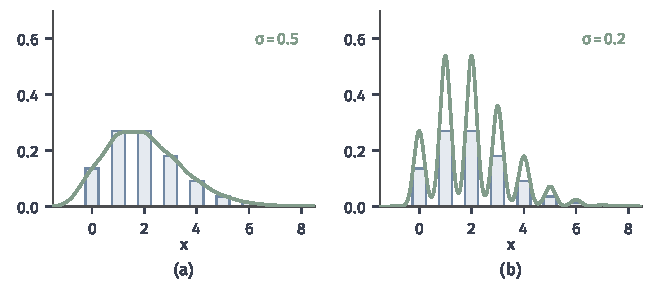
\includegraphics[width=112mm]{figures/07-probability/03-probability-limits/matplotlib/weak-gaussian-smoothing/figure.pdf}
 \caption{高斯平滑。浅蓝柱为$\operatorname{Poisson}(2)$在$k=0,\dots,7$的质量。曲线是由式~\eqref{eq:weak-smoothed-density}对特征函数数值积分得到的平滑密度$f_\sigma$：(a)$\sigma=0.5$（绿）；(b)$\sigma=0.2$（绿）。脚本同时按“各原子处放一个高斯小包”直接计算并核对两种结果相同。}
 \label{fig:weak-gaussian-smoothing}
\end{BookInlineFigure}

\paragraph{反演公式}
若$\phi_{\bm{X}}$本身在$\mathbb{R}^{d}$上可积，可以在式~\eqref{eq:weak-smoothed-density}中直接令$\sigma\to0$：被积函数被可积的$\lvert\phi_{\bm{X}}\rvert$控制，由支配收敛定理，$f_\sigma$一致收敛到
\begin{equation}
 f(\bm{x})=\frac{1}{(2\pi)^{d}}\int_{\mathbb{R}^{d}}\mathrm{e}^{-\mathrm{i}\langle\bm{t},\bm{x}\rangle}\,\phi_{\bm{X}}(\bm{t})\,\mathrm{d}\bm{t}
 \label{eq:weak-inversion}
\end{equation}
（积分变量换成了$\bm{t}=-\bm{s}$），这就是\term{反演公式}（inversion formula）。对连续且支撑有界的函数$h$，一方面$\mathbb{E}[h(\bm{X}+\sigma\bm{Z})]$等于$\int hf_\sigma$，趋于$\int hf$；另一方面由定理~\ref{thm:weak-prob-implies-dist}，它趋于$\mathbb{E}[h(\bm{X})]$。用这样的$h$从上方逼近闭长方体的示性函数，与引理~\ref{lem:weak-uniqueness}同样的单调极限说明，$\bm{X}$有连续密度$f$。这与\BookChapterRef{chap:fourier-transform}{卷四第14章“Fourier变换”}的$L^{1}$反演定理是同一件事，那里的约定在指数中带有$2\pi$，常数因而不同。

用反演公式可以求出一个不易直接积分的特征函数。$\operatorname{Laplace}(0,1)$的密度为$\frac12\mathrm{e}^{-\lvert x\rvert}$，它对称，特征函数为
\[
 \int_0^{\infty}\mathrm{e}^{-x}\cos(tx)\,\mathrm{d}x=\frac{1}{1+t^{2}} .
\]
它可积，由式~\eqref{eq:weak-inversion}，
\[
 \frac12\mathrm{e}^{-\lvert x\rvert}=\frac{1}{2\pi}\int_{-\infty}^{\infty}\frac{\mathrm{e}^{-\mathrm{i}tx}}{1+t^{2}}\,\mathrm{d}t .
\]
交换$x$与$t$的名字，两边乘以$2$。右边的被积函数中，Cauchy密度对称，$\mathrm{e}^{-\mathrm{i}tx}$可以换成$\mathrm{e}^{\mathrm{i}tx}$，于是右边就是标准Cauchy分布（密度$1/(\pi(1+x^{2}))$）在$t$处的特征函数，它等于$\mathrm{e}^{-\lvert t\rvert}$。

Cauchy分布的特征函数在原点不可导，与它没有期望相符。它还说明式~\eqref{eq:weak-cf-sum}的逆命题不成立：设$X$服从标准Cauchy分布，取$Y=X$，则
\[
 \phi_{X+Y}(t)=\phi_X(2t)=\mathrm{e}^{-2\lvert t\rvert}=\phi_X(t)\,\phi_Y(t) ,
\]
乘积公式成立，而$X$与$Y$并不独立。

\paragraph{有界变量的矩}
第~\ref{chap:random-variable-moments}章提到，取值有界时全部矩决定分布。现在可以证明这一点。设$\lvert X\rvert\leq M$，在引理~\ref{lem:weak-exp-remainder}中取$x=tX$并取期望，
\[
 \Bigl\lvert\phi_X(t)-\sum_{j=0}^{m}\frac{(\mathrm{i}t)^{j}}{j!}\mathbb{E}[X^{j}]\Bigr\rvert\leq\frac{(\lvert t\rvert M)^{m+1}}{(m+1)!}\longrightarrow0\qquad(m\to\infty) .
\]
所以对每个$t$，
\[
 \phi_X(t)=\sum_{j\geq0}\frac{(\mathrm{i}t)^{j}}{j!}\mathbb{E}[X^{j}] .
\]
两个有界变量若各阶矩相同，特征函数就相同，由定理~\ref{thm:weak-cf-uniqueness}，分布也相同。第~\ref{sec:weak-mgf}节将把有界的条件放宽为指数矩有限，并看到不加条件时结论可能失败。

\subsection{连续性定理}
\label{sec:weak-cf-continuity}

现在回到弱收敛。$\cos\langle\bm{t},\bm{x}\rangle$与$\sin\langle\bm{t},\bm{x}\rangle$是有界连续函数，所以弱收敛时特征函数逐点收敛。反过来，若特征函数逐点收敛，分布是否弱收敛？还要排除质量逃逸。

先看反例。$X_n\sim\mathcal{N}(0,n)$的特征函数是$\mathrm{e}^{-nt^{2}/2}$，它在$t=0$处恒为$1$，在$t\neq0$处趋于$0$。逐点极限
\[
 \psi(t)=\begin{cases}1,&t=0,\\0,&t\neq0\end{cases}
\]
存在，但在原点不连续；而第~\ref{sec:weak-tightness}节已经看到，这列分布的质量逃向无穷远，没有弱极限。原点附近的特征函数对应低频，也就是大尺度的形状；质量跑远，正表现为低频部分的塌缩。下面的引理把这个直观写成不等式。

\begin{lemma}[由特征函数控制尾概率]
\label{lem:weak-cf-tail}
设$X$是实随机变量，$u>0$，则
\begin{equation}
 \mathbb{P}\bigl(\lvert X\rvert\geq2/u\bigr)\leq\frac1u\int_{-u}^{u}\bigl(1-\phi_X(t)\bigr)\,\mathrm{d}t .
 \label{eq:weak-cf-tail}
\end{equation}
右边是实数，因为$\phi_X$的虚部是奇函数，积分为零。
\end{lemma}

\begin{proof}
对固定的$x\neq0$，
\[
 \frac1u\int_{-u}^{u}\bigl(1-\mathrm{e}^{\mathrm{i}tx}\bigr)\,\mathrm{d}t=2-\frac{2\sin(ux)}{ux}=2\Bigl(1-\frac{\sin(ux)}{ux}\Bigr) ,
\]
$x=0$时左边为$0$。被积函数有界，由Fubini定理交换期望与积分，
\[
 \frac1u\int_{-u}^{u}\bigl(1-\phi_X(t)\bigr)\,\mathrm{d}t=2\,\mathbb{E}\Bigl[1-\frac{\sin(uX)}{uX}\Bigr] ,
\]
其中$uX=0$时方括号内取$0$。

对一切实数$y\neq0$有$\lvert\sin y/y\rvert\leq1$，所以$1-\sin y/y\geq0$；当$\lvert y\rvert\geq2$时$\lvert\sin y/y\rvert\leq1/\lvert y\rvert\leq1/2$，所以$1-\sin y/y\geq1/2$。于是
\[
 2\,\mathbb{E}\Bigl[1-\frac{\sin(uX)}{uX}\Bigr]\geq2\cdot\frac12\,\mathbb{P}\bigl(\lvert uX\rvert\geq2\bigr)=\mathbb{P}\bigl(\lvert X\rvert\geq2/u\bigr) .
\]
\end{proof}

\begin{theorem}[连续性定理]
\label{thm:weak-continuity}
设$P_n$是$\mathbb{R}^{d}$上的概率分布，特征函数为$\phi_n$。
\begin{enumerate}
 \item 若$P_n\xrightarrow{\mathrm{w}}P$，则$\phi_n(\bm{t})\to\phi_P(\bm{t})$对每个$\bm{t}$成立。
 \item 若$\phi_n(\bm{t})$对每个$\bm{t}$收敛到某个$\psi(\bm{t})$，并且$\psi$在$\bm{0}$处连续，则存在概率分布$P$，使$\psi=\phi_P$且$P_n\xrightarrow{\mathrm{w}}P$。
\end{enumerate}
\end{theorem}

\begin{proof}
(1)：对固定的$\bm{t}$，$\phi_n(\bm{t})$的实部与虚部是有界连续函数$\cos\langle\bm{t},\bm{x}\rangle$与$\sin\langle\bm{t},\bm{x}\rangle$的读数，由定义~\ref{def:weak-convergence}收敛。

(2)：分两步。第一步证明$\{P_n\}$胎紧，先看$d=1$。$\psi(0)=\lim\phi_n(0)=1$。任取$\varepsilon>0$，由$\psi$在原点连续，取$u>0$使$\lvert1-\psi(t)\rvert\leq\varepsilon/2$对$\lvert t\rvert\leq u$成立，于是
\[
 \Bigl\lvert\frac1u\int_{-u}^{u}\bigl(1-\psi(t)\bigr)\,\mathrm{d}t\Bigr\rvert\leq\varepsilon .
\]
$\lvert1-\phi_n\rvert\leq2$，由支配收敛定理，
\[
 \frac1u\int_{-u}^{u}\bigl(1-\phi_n(t)\bigr)\,\mathrm{d}t\longrightarrow\frac1u\int_{-u}^{u}\bigl(1-\psi(t)\bigr)\,\mathrm{d}t .
\]
所以存在$N$，当$n\geq N$时左边小于$2\varepsilon$，由引理~\ref{lem:weak-cf-tail}，
\[
 P_n\bigl(\lvert x\rvert\geq2/u\bigr)<2\varepsilon,\qquad n\geq N .
\]
前$N-1$个分布各自胎紧，与之合并，整列胎紧。

$d>1$时，第$j$个坐标$x_j=\langle\bm{e}_j,\bm{x}\rangle$在$P_n$下的特征函数是$s\mapsto\phi_n(s\bm{e}_j)$，它逐点趋于$s\mapsto\psi(s\bm{e}_j)$，后者在$0$处连续。由一维的结论，每个坐标的分布胎紧。再由
\[
 P_n\bigl(\lVert\bm{x}\rVert_2>r\bigr)\leq\sum_{j=1}^{d}P_n\bigl(\lvert x_j\rvert>r/\sqrt{d}\bigr) ,
\]
$\{P_n\}$胎紧。

第二步识别极限。由定理~\ref{thm:weak-prokhorov}，$\{P_n\}$的每个子列都有进一步的子列弱收敛。设某个子列$P_{n_k}\xrightarrow{\mathrm{w}}Q$，由(1)，$\phi_Q=\lim\phi_{n_k}=\psi$。所以每个子列极限的特征函数都是$\psi$，由定理~\ref{thm:weak-cf-uniqueness}，它们是同一个分布，记作$P$。由引理~\ref{lem:weak-subsequence}，$P_n\xrightarrow{\mathrm{w}}P$，并且$\phi_P=\psi$。
\end{proof}

定理~\ref{thm:weak-continuity}常称为\term{Lévy连续性定理}（Lévy continuity theorem）。(2)的两步对应第~\ref{sec:weak-tightness}节末尾所说的两件事。原点连续性只用在第一步：它通过引理~\ref{lem:weak-cf-tail}保证质量不逃逸。识别极限则交给唯一性定理。结论中$\psi$是特征函数这一点也是证明的产物，并不需要事先知道。

\paragraph{再看二项分布到Poisson分布}
用连续性定理可以不经质量表重新证明$\operatorname{Bin}(n,2/n)\xrightarrow{\mathrm{w}}\operatorname{Poisson}(2)$。需要一个比较乘积的引理，它在下一章的中心极限定理中也要用到。

\begin{lemma}[乘积之差]
\label{lem:weak-product-difference}
设复数$a_1,\dots,a_n$与$b_1,\dots,b_n$的模都不超过$1$，则
\begin{equation}
 \Bigl\lvert\prod_{j=1}^{n}a_j-\prod_{j=1}^{n}b_j\Bigr\rvert\leq\sum_{j=1}^{n}\lvert a_j-b_j\rvert .
 \label{eq:weak-product-difference}
\end{equation}
\end{lemma}

\begin{proof}
$n=1$时是等式。设$n-1$时成立，把差拆成两部分：
\[
 \prod_{j=1}^{n}a_j-\prod_{j=1}^{n}b_j=a_n\Bigl(\prod_{j<n}a_j-\prod_{j<n}b_j\Bigr)+(a_n-b_n)\prod_{j<n}b_j .
\]
$\lvert a_n\rvert\leq1$，$\lvert\prod_{j<n}b_j\rvert\leq1$，由三角不等式与归纳假设即得。
\end{proof}

设$X_n\sim\operatorname{Bin}(n,2/n)$，记$z=2(\mathrm{e}^{\mathrm{i}t}-1)$，则
\[
 \phi_{X_n}(t)=\Bigl(1+\frac zn\Bigr)^{n},\qquad\exp\bigl(2(\mathrm{e}^{\mathrm{i}t}-1)\bigr)=\bigl(\mathrm{e}^{z/n}\bigr)^{n} .
\]
$n\geq2$时，$1+z/n=(1-2/n)+(2/n)\mathrm{e}^{\mathrm{i}t}$是单位圆盘中两点的凸组合，模不超过$1$；$z$的实部$2(\cos t-1)\leq0$，所以$\lvert\mathrm{e}^{z/n}\rvert\leq1$。

由引理~\ref{lem:weak-product-difference}，
\[
 \bigl\lvert\phi_{X_n}(t)-\mathrm{e}^{z}\bigr\rvert\leq n\,\Bigl\lvert1+\frac zn-\mathrm{e}^{z/n}\Bigr\rvert .
\]
对$\lvert w\rvert\leq1$，由幂级数，
\[
 \lvert\mathrm{e}^{w}-1-w\rvert\leq\sum_{k\geq2}\frac{\lvert w\rvert^{k}}{k!}\leq\lvert w\rvert^{2}(\mathrm{e}-2)\leq\lvert w\rvert^{2} .
\]
$\lvert z\rvert\leq4$，取$n\geq4$与$w=z/n$，得到
\[
 \bigl\lvert\phi_{X_n}(t)-\exp\bigl(2(\mathrm{e}^{\mathrm{i}t}-1)\bigr)\bigr\rvert\leq n\cdot\frac{\lvert z\rvert^{2}}{n^{2}}\leq\frac{16}{n} .
\]
所以特征函数收敛到$\operatorname{Poisson}(2)$的特征函数，后者连续，由连续性定理即得弱收敛。

以$t=\pi$为例，$z=-4$，$\phi_{X_n}(\pi)=(1-4/n)^{n}$。$n=10$与$n=40$时依次为
\[
 0.6^{10}\approx0.00605,\qquad0.9^{40}\approx0.0148 ,
\]
极限为$\mathrm{e}^{-4}\approx0.0183$。图~\ref{fig:weak-continuity}(a)画出特征函数实部的收敛；(b)是$\mathcal{N}(0,n)$的反例，极限在原点断开。

\begin{BookInlineFigure}
 \centering
 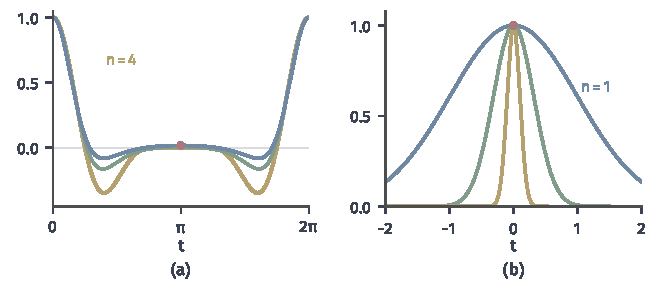
\includegraphics[width=112mm]{figures/07-probability/03-probability-limits/matplotlib/weak-continuity/figure.pdf}
 \caption{连续性定理的两种情形。(a)$\operatorname{Bin}(n,2/n)$特征函数的实部，$n=4$（黄）、$10$（绿），蓝线为$\operatorname{Poisson}(2)$的$\operatorname{Re}\exp(2(\mathrm{e}^{\mathrm{i}t}-1))$，红点为$t=\pi$处的极限$\mathrm{e}^{-4}$。(b)$\mathcal{N}(0,n)$的特征函数$\mathrm{e}^{-nt^2/2}$，$n=1$（蓝）、$10$（绿）、$100$（黄），逐点极限在原点为$1$（红点）、其余为$0$。}
 \label{fig:weak-continuity}
\end{BookInlineFigure}


\section{矩母函数}
\label{sec:weak-mgf}

第~\ref{chap:tail-probabilities}章用矩母函数$M_X(t)=\mathbb{E}[\mathrm{e}^{tX}]$给出尾概率的指数界，并提到它在一定条件下决定分布。它与特征函数只差一个$\mathrm{i}$：把$\mathrm{e}^{\mathrm{i}tX}$换成$\mathrm{e}^{tX}$。可是这一换，被积函数不再有界，$M_X(t)$可能是$+\infty$。本节研究它在哪里有限，有限时能做什么，以及它与特征函数的分工。

\paragraph{有限的范围}
记$D_X=\{t\in\mathbb{R}:M_X(t)<\infty\}$。总有$0\in D_X$。$D_X$是一个区间：若$t_1,t_2\in D_X$，$0<\theta<1$，由$t\mapsto\mathrm{e}^{tx}$的凸性，
\[
 \mathrm{e}^{(\theta t_1+(1-\theta)t_2)x}\leq\theta\,\mathrm{e}^{t_1x}+(1-\theta)\,\mathrm{e}^{t_2x} ,
\]
取期望知$\theta t_1+(1-\theta)t_2\in D_X$。这个区间可以是整条实轴、半直线、有界区间，也可以只有一个点。

几个例子。$\mathcal{N}(0,1)$与$\operatorname{Poisson}(\lambda)$的矩母函数分别是$\mathrm{e}^{t^{2}/2}$与$\exp(\lambda(\mathrm{e}^{t}-1))$，对一切$t$有限。$\operatorname{Exp}(1)$的矩母函数是$1/(1-t)$，$D_X=(-\infty,1)$。标准Cauchy分布的密度只按$x^{-2}$衰减，$t\neq0$时$\mathrm{e}^{tx}$在一侧指数增长，积分发散，$D_X=\{0\}$。$D_X$能否包含$0$的一个邻域，取决于两侧尾部是否都至少按指数衰减。

\paragraph{生成矩}
在$0$的邻域上有限时，矩母函数配得上它的名字。

\begin{theorem}[矩母函数与矩]
\label{thm:weak-mgf-moments}
设存在$t_0>0$，使$M_X(t)<\infty$对$\lvert t\rvert<t_0$成立。则
\begin{enumerate}
 \item 对每个整数$k\geq0$与$0<t<t_0$，
 \begin{equation}
 \mathbb{E}\bigl[\lvert X\rvert^{k}\bigr]\leq\frac{k!}{t^{k}}\bigl(M_X(t)+M_X(-t)\bigr)<\infty ;
 \label{eq:weak-mgf-moment-bound}
 \end{equation}
 \item 对$\lvert t\rvert<t_0$，$M_X(t)=\sum_{k\geq0}t^{k}\,\mathbb{E}[X^{k}]/k!$；
 \item $M_X$在$(-t_0,t_0)$上任意次可导，$M_X^{(k)}(0)=\mathbb{E}[X^{k}]$。
\end{enumerate}
\end{theorem}

\begin{proof}
(1)：对$t>0$，$\mathrm{e}^{t\lvert x\rvert}$的幂级数每一项非负，保留第$k$项，得
\[
 \frac{t^{k}\lvert x\rvert^{k}}{k!}\leq\mathrm{e}^{t\lvert x\rvert}\leq\mathrm{e}^{tx}+\mathrm{e}^{-tx} ,
\]
第二个不等号是因为$\mathrm{e}^{t\lvert x\rvert}$就是$\mathrm{e}^{tx}$与$\mathrm{e}^{-tx}$中较大的一个。代入$X$并取期望即得。

(2)：部分和满足
\[
 \Bigl\lvert\sum_{k=0}^{m}\frac{(tX)^{k}}{k!}\Bigr\rvert\leq\mathrm{e}^{\lvert t\rvert\lvert X\rvert}\leq\mathrm{e}^{tX}+\mathrm{e}^{-tX} ,
\]
右边可积，部分和逐点趋于$\mathrm{e}^{tX}$。由支配收敛定理，期望与求和可以交换。

(3)：由(2)，$M_X$在$(-t_0,t_0)$上是收敛的幂级数，可以逐项求导任意次（可参考\BookChapterRef{chap:univariate-differentiation}{卷一第6章“一元函数的微分”}），$t^{k}$的系数乘以$k!$就是$k$阶导数在$0$处的值。
\end{proof}

这回答了第~\ref{chap:tail-probabilities}章留下的问题：逐项取期望的依据是支配收敛定理，控制函数是$\mathrm{e}^{tX}+\mathrm{e}^{-tX}$，它的可积性正来自$0$两侧的有限性。例如$X\sim\operatorname{Exp}(1)$，$1/(1-t)=\sum_{k\geq0}t^{k}$对$\lvert t\rvert<1$成立，比较系数得
\[
 \mathbb{E}[X^{k}]=k!,\qquad k=0,1,2,\dots .
\]

\paragraph{识别分布}
矩母函数在$0$的邻域上相同，能否推出分布相同？借助特征函数可以证明。思路是：矩母函数相同推出各阶矩相同；指数矩有限又使特征函数在每一点附近都能用Taylor级数表示，于是可以从原点出发，一段一段地推出两个特征函数处处相同。

\begin{theorem}[矩母函数确定分布]
\label{thm:weak-mgf-uniqueness}
设存在$t_0>0$，使$M_X(t)=M_Y(t)<\infty$对$\lvert t\rvert<t_0$成立，则$P_X=P_Y$。
\end{theorem}

\begin{proof}
取$0<r<t_0$。先证明：对每个$s\in\mathbb{R}$与$\lvert h\rvert\leq r$，
\begin{equation}
 \phi_X(s+h)=\sum_{k\geq0}\frac{\phi_X^{(k)}(s)}{k!}h^{k} .
 \label{eq:weak-cf-taylor-series}
\end{equation}
由定理~\ref{thm:weak-mgf-moments}，各阶矩有限，式~\eqref{eq:weak-cf-derivatives}给出各阶导数$\phi_X^{(k)}(s)$的期望表示。在引理~\ref{lem:weak-exp-remainder}中取$x=hX$，乘以$\mathrm{e}^{\mathrm{i}sX}$并取期望，
\[
 \Bigl\lvert\phi_X(s+h)-\sum_{k=0}^{m}\frac{\phi_X^{(k)}(s)}{k!}h^{k}\Bigr\rvert\leq\frac{\mathbb{E}\bigl[\lvert hX\rvert^{m+1}\bigr]}{(m+1)!} .
\]
由单调收敛定理，
\[
 \sum_{m\geq0}\frac{\mathbb{E}[\lvert hX\rvert^{m}]}{m!}=\mathbb{E}\bigl[\mathrm{e}^{\lvert h\rvert\lvert X\rvert}\bigr]\leq M_X(r)+M_X(-r)<\infty ,
\]
级数收敛，通项趋于零，于是式~\eqref{eq:weak-cf-taylor-series}成立。对$Y$同样成立。

由定理~\ref{thm:weak-mgf-moments}(3)，$X$与$Y$的各阶矩相同，由式~\eqref{eq:weak-cf-derivatives}，$\phi_X$与$\phi_Y$在原点的各阶导数相同。在式~\eqref{eq:weak-cf-taylor-series}中取$s=0$，得$\phi_X=\phi_Y$在$[-r,r]$上成立。

再逐段推广。设已知$\phi_X=\phi_Y$在开区间$(-a,a)$上成立，$a\geq r$。取$s=a-r/2$，它在$(-a,a)$内部，两个函数在$s$的一个邻域上相同，所以各阶导数在$s$处相同。由式~\eqref{eq:weak-cf-taylor-series}，两个函数在$[s-r,s+r]$上相同，右端点$a+r/2$超过了$a$。对$-s$作同样的论证。于是$\phi_X=\phi_Y$在$(-a-r/2,a+r/2)$上成立，重复下去覆盖整条实轴。由定理~\ref{thm:weak-cf-uniqueness}，$P_X=P_Y$。
\end{proof}

特征函数在这里仍是识别的工具，矩母函数的作用是保证特征函数可以由原点处的各阶导数完全决定。类似地可以证明：若$M_{X_n}(t)\to M_X(t)$对$0$的某个邻域内的每个$t$成立，且右边有限，则$X_n\xrightarrow{\mathrm{d}}X$；证明要先由矩母函数的一致有界得到胎紧，再用第~\ref{sec:weak-integral-limits}节的方法识别极限，可查阅~\scite{math-kallenberg2021probability}。独立和的矩母函数也是各项矩母函数之积，只要各项在相应的$t$处有限，证明与定理~\ref{thm:weak-cf-independent}相同。

\paragraph{对数正态分布}
所有矩都有限，是否就保证矩母函数在$0$的邻域有限？对数正态分布给出否定的回答。设$Z\sim\mathcal{N}(0,1)$，$Y=\mathrm{e}^{Z}$。由高斯的矩母函数，各阶矩都有限：
\[
 \mathbb{E}[Y^{k}]=\mathbb{E}\bigl[\mathrm{e}^{kZ}\bigr]=\mathrm{e}^{k^{2}/2},\qquad k=0,1,2,\dots .
\]
可是对任意$t>0$，
\[
 M_Y(t)=\int_{-\infty}^{\infty}\frac{1}{\sqrt{2\pi}}\exp\Bigl(t\,\mathrm{e}^{z}-\frac{z^{2}}{2}\Bigr)\,\mathrm{d}z=+\infty ,
\]
因为$z\to\infty$时$t\,\mathrm{e}^{z}$比$z^{2}/2$增长得快，被积函数趋于无穷。$t\leq0$时$\mathrm{e}^{tY}\leq1$，$M_Y(t)$有限。所以$D_Y=(-\infty,0]$，不含$0$的邻域，定理~\ref{thm:weak-mgf-uniqueness}不能用。

这不只是证明方法的缺陷：确实存在另一个分布与$Y$有完全相同的各阶矩。记$f$为$Y$的密度，对$\lvert a\rvert\leq1$令
\[
 f_a(y)=f(y)\bigl(1+a\sin(2\pi\ln y)\bigr),\qquad y>0 .
\]
$f_a\geq0$。下面验证它的各阶矩与$f$相同，$k=0$时即得$f_a$是密度。

只需证明对每个$k\geq0$，
\[
 \int_0^{\infty}y^{k}f(y)\sin(2\pi\ln y)\,\mathrm{d}y=0 .
\]
用$y=\mathrm{e}^{z}$换元，左边等于$\mathbb{E}[\mathrm{e}^{kZ}\sin(2\pi Z)]$。对指数配方，$kz-z^{2}/2=k^{2}/2-(z-k)^{2}/2$，所以
\[
 \mathrm{e}^{kz}\varphi(z)=\mathrm{e}^{k^{2}/2}\varphi(z-k) ,
\]
于是
\[
 \mathbb{E}\bigl[\mathrm{e}^{kZ}\sin(2\pi Z)\bigr]=\mathrm{e}^{k^{2}/2}\,\mathbb{E}\bigl[\sin\bigl(2\pi(Z+k)\bigr)\bigr]=\mathrm{e}^{k^{2}/2}\,\mathbb{E}\bigl[\sin(2\pi Z)\bigr]=0 .
\]
第二个等号用了$k$是整数、正弦的周期是$2\pi$；最后一个等号是因为$\sin(2\pi z)\varphi(z)$是奇函数。

$a\neq0$时$f_a$与$f$是不同的密度，各阶矩却全部相同，图~\ref{fig:weak-lognormal}画出了$a=1/2$的情形。这就是第~\ref{chap:random-variable-moments}章提到的情形：尾部较重时，全部矩也不能确定分布。两者的特征函数当然不同，由定理~\ref{thm:weak-cf-uniqueness}，这是必然的。

\begin{BookInlineFigure}
 \centering
 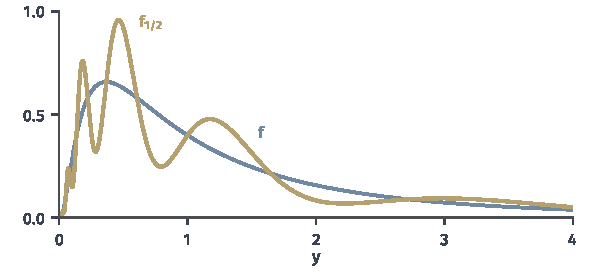
\includegraphics[width=100mm]{figures/07-probability/03-probability-limits/matplotlib/weak-lognormal/figure.pdf}
 \caption{各阶矩相同的两个密度。蓝线为对数正态密度$f$，黄线为$f_{1/2}(y)=f(y)(1+\frac12\sin(2\pi\ln y))$。脚本用数值积分核对了二者的前四阶矩都等于$\mathrm{e}^{k^2/2}$。}
 \label{fig:weak-lognormal}
\end{BookInlineFigure}

\paragraph{两种表示的分工}
下表比较两种变换。特征函数总存在，识别分布与刻画弱收敛都不需要附加条件；矩母函数是实值的，便于计算矩和尾部的指数界，但只有在$0$的邻域上有限时才能用于识别。下一章证明中心极限定理时只假定方差有限，矩母函数可能处处无穷（例如$t$分布），所以证明用特征函数，不以矩母函数存在作为前提。

\begin{BookInlineTable}
 \centering
 \caption{特征函数与矩母函数}
 \label{tab:weak-cf-mgf}
 \begin{tabular}{@{}lll@{}}
 \toprule
 & 特征函数$\phi_X(t)$ & 矩母函数$M_X(t)$\\
 \midrule
 存在范围 & 一切$t$，模不超过$1$ & 区间$D_X$，可能只有$\{0\}$\\
 读出矩 & $k$阶矩有限时求$k$次导 & $0$的邻域有限时全部矩\\
 识别分布 & 无条件 & 需$0$的邻域有限\\
 收敛判据 & 连续性定理 & 需$0$的邻域上收敛\\
 独立和 & 乘积 & 乘积（在有限处）\\
 \bottomrule
 \end{tabular}
\end{BookInlineTable}


\section{连续映射}
\label{sec:weak-continuous-mapping}

已知$X_n\xrightarrow{\mathrm{d}}X$，常常还要知道$X_n^{2}$、$\mathrm{e}^{X_n}$、$\mathbf{1}_{\{X_n>a\}}$或$1/X_n$的极限。对每个$X_n$作同一个确定的变换$g$，极限能否随之传递？若$g$连续，答案几乎写在定义里：对$f\in C_b$，复合$f\circ g$仍是有界连续函数，所以
\[
 \mathbb{E}\bigl[f(g(\bm{X}_n))\bigr]=\mathbb{E}\bigl[(f\circ g)(\bm{X}_n)\bigr]\longrightarrow\mathbb{E}\bigl[(f\circ g)(\bm{X})\bigr]=\mathbb{E}\bigl[f(g(\bm{X}))\bigr] .
\]

实际要用的$g$常有不连续点：阈值的示性函数在阈值处跳跃，倒数在$0$处没有定义。下面的定理允许$g$有不连续点，只要极限分布不把质量放在那里。

\begin{theorem}[连续映射定理]
\label{thm:weak-continuous-mapping}
设$\bm{X}_n\xrightarrow{\mathrm{d}}\bm{X}$，$\bm{X}_n,\bm{X}$取值于$\mathbb{R}^{d}$。设$g:\mathbb{R}^{d}\to\mathbb{R}^{k}$为Borel可测映射，$D_g$为它的不连续点集。若$\mathbb{P}(\bm{X}\in D_g)=0$，则$g(\bm{X}_n)\xrightarrow{\mathrm{d}}g(\bm{X})$。
\end{theorem}

\begin{proof}
可以证明$D_g$是Borel集，所以$\mathbb{P}(\bm{X}\in D_g)$有意义。用Portmanteau定理的(3)验证。取$\mathbb{R}^{k}$中的闭集$F$，记$\overline{g^{-1}(F)}$为原像的闭包。

先说明$\overline{g^{-1}(F)}\subset g^{-1}(F)\cup D_g$。设$\bm{x}$在闭包中，取$\bm{x}_m\in g^{-1}(F)$，$\bm{x}_m\to\bm{x}$。若$g$在$\bm{x}$处连续，则$g(\bm{x})=\lim g(\bm{x}_m)$，而$g(\bm{x}_m)\in F$，$F$闭，所以$g(\bm{x})\in F$，即$\bm{x}\in g^{-1}(F)$。否则$\bm{x}\in D_g$。

于是，由原像的闭包是闭集，以及$\bm{X}_n\xrightarrow{\mathrm{d}}\bm{X}$与Portmanteau定理的(3)，
\[
 \begin{aligned}
 \limsup_{n\to\infty}\mathbb{P}\bigl(g(\bm{X}_n)\in F\bigr)
 &\leq\limsup_{n\to\infty}\mathbb{P}\bigl(\bm{X}_n\in\overline{g^{-1}(F)}\bigr)
 \leq\mathbb{P}\bigl(\bm{X}\in\overline{g^{-1}(F)}\bigr)\\
 &\leq\mathbb{P}\bigl(\bm{X}\in g^{-1}(F)\bigr)+\mathbb{P}(\bm{X}\in D_g)=\mathbb{P}\bigl(g(\bm{X})\in F\bigr) .
 \end{aligned}
\]
再用一次Portmanteau定理即得结论。
\end{proof}

定理~\ref{thm:weak-continuous-mapping}通称\term{连续映射定理}（continuous mapping theorem）。条件$\mathbb{P}(\bm{X}\in D_g)=0$只涉及极限$\bm{X}$，与$\bm{X}_n$是否把质量放在$D_g$上无关。这与Portmanteau定理(5)的边界条件是同一种要求：示性函数$\mathbf{1}_A$的不连续点集正是$\partial A$。

\paragraph{阈值}
设$g(x)=\mathbf{1}_{\{x>1/2\}}$，$D_g=\{1/2\}$。对格点均匀分布，$U_n\xrightarrow{\mathrm{d}}U\sim\operatorname{Unif}(0,1)$，且$\mathbb{P}(U=1/2)=0$，所以$\mathbf{1}_{\{U_n>1/2\}}\xrightarrow{\mathrm{d}}\operatorname{Bern}(1/2)$。直接计算也是如此：$\mathbb{P}(U_n>1/2)=1-\lfloor n/2\rfloor/n\to1/2$。

换成$\delta_{1/n}\to\delta_0$与阈值$0$，$g(x)=\mathbf{1}_{\{x>0\}}$，则$g(1/n)=1$恒成立，而$g(0)=0$。极限分布的全部质量都在$D_g=\{0\}$上，条件不满足，结论确实失败。图~\ref{fig:weak-threshold-mapping}并列了这两种情形。

\begin{BookInlineFigure}
 \centering
 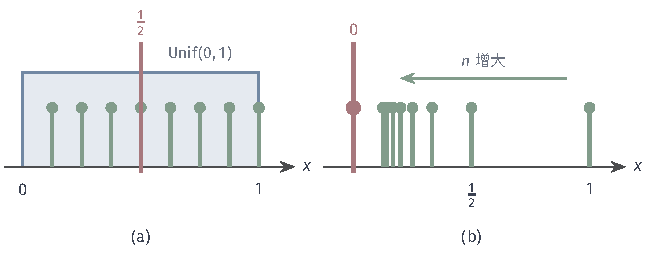
\includegraphics[width=110.6mm]{figures/07-probability/03-probability-limits/tikz/weak-threshold-mapping/figure.pdf}
 \caption{阈值映射与极限质量的位置。(a)格点均匀分布$U_8$的质点（绿）与极限$\operatorname{Unif}(0,1)$的密度（浅蓝），阈值$1/2$（红色竖线）处$U_8$有质量而极限没有，阈值右侧的概率收敛到$1/2$。(b)$\delta_{1/n}$的质点（绿）从右侧逼近阈值$0$，极限$\delta_0$（红点）恰好落在阈值上，$\mathbf{1}_{\{X_n>0\}}$恒为$1$，极限却是$0$。}
 \label{fig:weak-threshold-mapping}
\end{BookInlineFigure}

\paragraph{倒数}
令$g(x)=1/x$（$x\neq0$），$g(0)=0$，则$D_g=\{0\}$。若$X_n\xrightarrow{\mathrm{d}}X$且$\mathbb{P}(X=0)=0$，则$1/X_n\xrightarrow{\mathrm{d}}1/X$。$g(0)$取什么值无关紧要，它只影响$X_n=0$的样本，而极限分布不关心那里。

仍以格点均匀分布为例，$\mathbb{P}(U=0)=0$，所以$1/U_n\xrightarrow{\mathrm{d}}1/U$。极限的右尾为
\[
 \mathbb{P}(1/U>y)=\mathbb{P}(U<1/y)=\frac1y,\qquad y\geq1 ,
\]
这是第~\ref{chap:tail-probabilities}章参数为$1$的Pareto分布，没有期望。直接计算，$U_n<1/y$的格点是$k<n/y$，个数为$\lceil n/y\rceil-1$，于是
\[
 \mathbb{P}(1/U_n>y)=\frac{\lceil n/y\rceil-1}{n}\longrightarrow\frac1y .
\]
注意每个$1/U_n$都不超过$n$，有界；极限却是重尾分布。图~\ref{fig:weak-reciprocal}(a)画出这一收敛。

分母趋于零时条件就会失效。设$X_n=(-1)^{n}/n$，则$X_n\xrightarrow{\mathrm{d}}0$，极限把全部质量放在$D_g$上。$1/X_n=(-1)^{n}n$在$\pm\infty$之间来回跳，没有任何弱极限。即使取$X_n\sim\mathcal{N}(0,1/n^{2})$这样处处没有原子的分布，$1/X_n$的分布也是$1/X_1$的分布按$n$倍放大，质量逃向无穷远，见图~\ref{fig:weak-reciprocal}(b)。

\begin{BookInlineFigure}
 \centering
 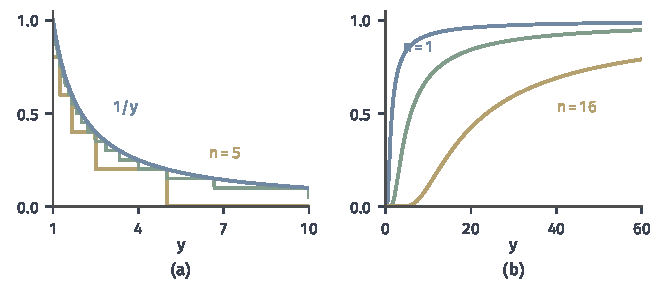
\includegraphics[width=112mm]{figures/07-probability/03-probability-limits/matplotlib/weak-reciprocal/figure.pdf}
 \caption{倒数映射。(a)$\mathbb{P}(1/U_n>y)$，$n=5$（黄）与$n=20$（绿），蓝线为极限$1/y$。(b)$X_n\sim\mathcal{N}(0,1/n^2)$时$\lvert1/X_n\rvert$的分布函数，$n=1$（蓝）、$4$（绿）、$16$（黄），曲线整体右移，质量逃向无穷远。}
 \label{fig:weak-reciprocal}
\end{BookInlineFigure}

连续映射定理处理的是同一个确定变换。若变换本身也随$n$变化，例如$g_n(x)=x+1/n$，则要另外论证；若变换涉及两个随机变量，例如$X_n+Y_n$，则需要$(X_n,Y_n)$作为一个随机向量的极限，这是下一节的问题。


\section{联合收敛}
\label{sec:weak-joint}

设$X_n\xrightarrow{\mathrm{d}}X$，$Y_n\xrightarrow{\mathrm{d}}Y$。$X_n+Y_n$的极限是什么？这个问题在只知道两个边缘极限时没有答案，因为$X+Y$的分布取决于$X$与$Y$怎样配对，而边缘分布不含配对的信息。本节先把联合收敛与边缘收敛分开，再给出两类常用的判据：方向投影，以及一个分量趋于常量的情形。有了联合极限，上一节的连续映射定理就可以处理和、积与比。

\subsection{边缘收敛与联合收敛}
\label{sec:weak-marginal-joint}

设$(\bm{X}_n,\bm{Y}_n)$是取值于$\mathbb{R}^{d}\times\mathbb{R}^{k}$的随机向量，即每个$n$下$\bm{X}_n$与$\bm{Y}_n$定义在同一个概率空间上。联合收敛$(\bm{X}_n,\bm{Y}_n)\xrightarrow{\mathrm{d}}(\bm{X},\bm{Y})$就是这个$(d+k)$维随机向量的依分布收敛。坐标投影$(\bm{x},\bm{y})\mapsto\bm{x}$连续，由连续映射定理，联合收敛推出$\bm{X}_n\xrightarrow{\mathrm{d}}\bm{X}$与$\bm{Y}_n\xrightarrow{\mathrm{d}}\bm{Y}$。

反过来不成立。设$Z\sim\mathcal{N}(0,1)$，令
\[
 X_n=Z,\qquad Y_n=(-1)^{n}Z .
\]
$-Z$也服从$\mathcal{N}(0,1)$，所以两个边缘分布对每个$n$都是$\mathcal{N}(0,1)$，边缘平凡地收敛。联合分布却在两种之间交替：偶数$n$时$(Z,Z)$落在直线$y=x$上，奇数$n$时$(Z,-Z)$落在$y=-x$上。取有界连续函数$f(x,y)=\min(1,\lvert x-y\rvert)$，偶数项的读数为$0$，奇数项为$\mathbb{E}[\min(1,2\lvert Z\rvert)]>0$，所以联合分布没有极限。图~\ref{fig:weak-pairings}画出这两种配对，以及同样边缘下的第三种配对：独立。

\begin{BookInlineFigure}
 \centering
 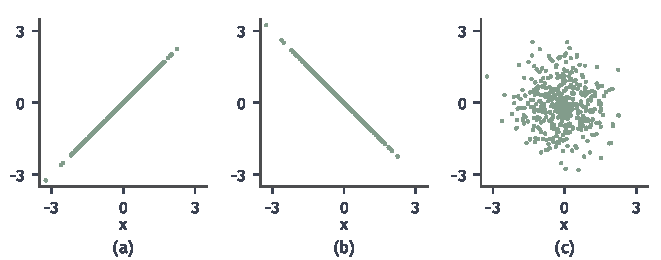
\includegraphics[width=112mm]{figures/07-probability/03-probability-limits/matplotlib/weak-pairings/figure.pdf}
 \caption{边缘相同、配对不同。三幅图各有$400$个样本点（种子$7$），两个坐标的边缘分布都是$\mathcal{N}(0,1)$。(a)$(Z,Z)$；(b)$(Z,-Z)$；(c)$(Z,Z')$，$Z'$与$Z$独立同分布。}
 \label{fig:weak-pairings}
\end{BookInlineFigure}

\paragraph{各分量独立的情形}
若对每个$n$，$\bm{X}_n$与$\bm{Y}_n$独立，配对方式就被固定下来，边缘收敛足以推出联合收敛。

\begin{theorem}[独立分量的联合极限]
\label{thm:weak-independent-joint}
设对每个$n$，$\bm{X}_n$与$\bm{Y}_n$定义在同一概率空间上且相互独立，$\bm{X}_n\xrightarrow{\mathrm{d}}\bm{X}$，$\bm{Y}_n\xrightarrow{\mathrm{d}}\bm{Y}$。则$(\bm{X}_n,\bm{Y}_n)\xrightarrow{\mathrm{d}}(\bm{X},\bm{Y})$，其中$\bm{X}$与$\bm{Y}$独立，即极限分布是$P_{\bm{X}}$与$P_{\bm{Y}}$的乘积。
\end{theorem}

\begin{proof}
由式~\eqref{eq:weak-cf-joint-independent}与连续性定理的(1)，
\[
 \phi_{(\bm{X}_n,\bm{Y}_n)}(\bm{s},\bm{t})=\phi_{\bm{X}_n}(\bm{s})\,\phi_{\bm{Y}_n}(\bm{t})\longrightarrow\phi_{\bm{X}}(\bm{s})\,\phi_{\bm{Y}}(\bm{t}) .
\]
取$\bm{X}$与$\bm{Y}$独立，右边正是$(\bm{X},\bm{Y})$的特征函数，它连续。由连续性定理的(2)，结论成立。
\end{proof}

定理只要求同一个$n$下的两个分量独立，不要求不同$n$之间有任何关系；各个$n$甚至可以在不同的概率空间上。例如每个$n$下独立地取$X_n\sim\operatorname{Bin}(n,2/n)$与格点均匀分布$U_n$，则$(X_n,U_n)$依分布收敛到$\operatorname{Poisson}(2)$与$\operatorname{Unif}(0,1)$的乘积分布。

\subsection{Cramér--Wold判据}
\label{sec:weak-cramer-wold}

一般的联合分布怎样检验？直接用多元特征函数可以，但常常更方便的是把向量投影到一个方向上，化为一维问题。投影$\langle\bm{a},\bm{X}\rangle$的特征函数在$1$处的值是
\[
 \phi_{\langle\bm{a},\bm{X}\rangle}(1)=\mathbb{E}\bigl[\mathrm{e}^{\mathrm{i}\langle\bm{a},\bm{X}\rangle}\bigr]=\phi_{\bm{X}}(\bm{a}) .
\]
所以多元特征函数在$\bm{a}$处的值，就是沿方向$\bm{a}$的一维投影的信息。知道所有方向的投影分布，就知道整个多元特征函数。

\begin{theorem}[Cramér--Wold判据]
\label{thm:weak-cramer-wold}
设$\bm{X}_n,\bm{X}$取值于$\mathbb{R}^{d}$。则$\bm{X}_n\xrightarrow{\mathrm{d}}\bm{X}$，当且仅当对每个$\bm{a}\in\mathbb{R}^{d}$，
\begin{equation}
 \langle\bm{a},\bm{X}_n\rangle\xrightarrow{\mathrm{d}}\langle\bm{a},\bm{X}\rangle .
 \label{eq:weak-cramer-wold}
\end{equation}
特别地，$\bm{X}$的分布由全部一维投影$\langle\bm{a},\bm{X}\rangle$的分布确定。
\end{theorem}

\begin{proof}
必要性：$\bm{x}\mapsto\langle\bm{a},\bm{x}\rangle$连续，由连续映射定理。充分性：由式~\eqref{eq:weak-cramer-wold}与连续性定理的(1)，对每个$\bm{a}$，
\[
 \phi_{\bm{X}_n}(\bm{a})=\phi_{\langle\bm{a},\bm{X}_n\rangle}(1)\longrightarrow\phi_{\langle\bm{a},\bm{X}\rangle}(1)=\phi_{\bm{X}}(\bm{a}) .
\]
极限$\phi_{\bm{X}}$连续，由连续性定理的(2)得$\bm{X}_n\xrightarrow{\mathrm{d}}\bm{X}$。最后一句：若$\bm{X}$与$\bm{Y}$的各个投影同分布，则$\phi_{\bm{X}}(\bm{a})=\phi_{\bm{Y}}(\bm{a})$对一切$\bm{a}$成立，由定理~\ref{thm:weak-cf-uniqueness}得$P_{\bm{X}}=P_{\bm{Y}}$。
\end{proof}

这个判据也称为\term{Cramér--Wold方法}（Cramér--Wold device）。判据要求所有方向，坐标方向只是$\bm{a}=\bm{e}_j$这$d$个特例，它们只给出边缘分布。上一小节的例子已经说明边缘不够；下面看一个固定的随机向量，它的坐标方向都是高斯，某个斜方向却不是。

\paragraph{联合高斯的判别}
第~\ref{chap:multivariate-distributions}章说过：若每个线性组合$\langle\bm{a},\bm{X}\rangle$都服从一元高斯分布（方差可以为$0$），则$\bm{X}$联合高斯。现在可以证明。每个坐标服从高斯分布，所以二阶矩有限，记$\bm{\mu}=\mathbb{E}[\bm{X}]$，$\bm{\Sigma}$为协方差矩阵。$\langle\bm{a},\bm{X}\rangle$的均值为$\langle\bm{a},\bm{\mu}\rangle$，方差为$\bm{a}^{\top}\bm{\Sigma}\bm{a}$，按假设它是高斯的，于是
\[
 \phi_{\bm{X}}(\bm{a})=\phi_{\langle\bm{a},\bm{X}\rangle}(1)=\exp\Bigl(\mathrm{i}\langle\bm{a},\bm{\mu}\rangle-\frac12\bm{a}^{\top}\bm{\Sigma}\bm{a}\Bigr) .
\]
这正是式~\eqref{eq:weak-mvn-cf}中$\mathcal{N}(\bm{\mu},\bm{\Sigma})$的特征函数，由定理~\ref{thm:weak-cf-uniqueness}，$\bm{X}\sim\mathcal{N}(\bm{\mu},\bm{\Sigma})$。

那一章还给出了只检查坐标方向不够的例子。$Z\sim\mathcal{N}(0,1)$，$S$以各$1/2$的概率取$\pm1$且与$Z$独立，$\bm{X}=(Z,SZ)$。两个坐标都服从$\mathcal{N}(0,1)$，由独立性，协方差$\mathbb{E}[SZ^{2}]$等于$\mathbb{E}[S]\,\mathbb{E}[Z^{2}]=0$。若$\bm{X}$联合高斯，它就是$\mathcal{N}(\bm{0},\bm{I}_2)$，方向$\bm{a}=(1,1)$上的投影应服从$\mathcal{N}(0,2)$。实际上
\[
 Z+SZ=(1+S)Z=\begin{cases}2Z,&S=1,\\0,&S=-1,\end{cases}
\]
它以概率$1/2$恰好等于$0$，不是高斯分布。图~\ref{fig:weak-cramer-wold}(a)是$\bm{X}$的样本，全部落在两条对角线上；(b)是这个斜方向投影的分布。

\begin{BookInlineFigure}
 \centering
 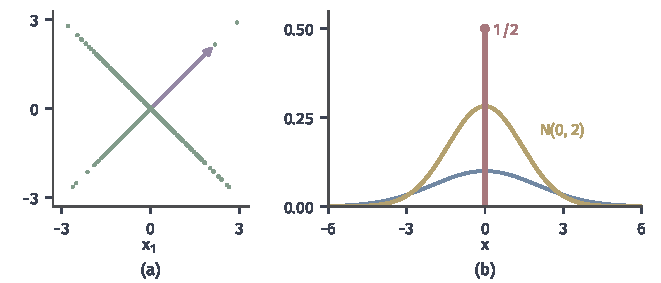
\includegraphics[width=112mm]{figures/07-probability/03-probability-limits/matplotlib/weak-cramer-wold/figure.pdf}
 \caption{坐标方向都是高斯，斜方向不是。(a)$\bm{X}=(Z,SZ)$的$600$个样本（种子$11$），两个边缘都是$\mathcal{N}(0,1)$，紫色箭头为方向$(1,1)$。(b)$Z+SZ$的分布：$0$处质量$1/2$的原子（红色竖线），其余质量的密度为$\frac12$乘$\mathcal{N}(0,4)$的密度（蓝）；黄线为假如联合高斯时应有的$\mathcal{N}(0,2)$密度。}
 \label{fig:weak-cramer-wold}
\end{BookInlineFigure}

Cramér--Wold判据适用于固定的有限维数$d$。下一章的多元中心极限定理正是用它把各个方向上的一维极限合成联合高斯极限。

\subsection{Slutsky定理}
\label{sec:weak-slutsky}

联合收敛有一个特别好用的情形：一个分量依分布收敛，另一个依概率趋于常量。常量没有随机性，不存在配对问题，所以边缘信息就够了。典型的场合是用一个依概率收敛的量替换未知的常数，例如第~\ref{chap:laws-of-large-numbers}章的大数律给出的样本平均。

\begin{theorem}[Slutsky定理]
\label{thm:weak-slutsky}
设对每个$n$，$\bm{X}_n$与$\bm{Y}_n$定义在同一概率空间上，分别取值于$\mathbb{R}^{d}$与$\mathbb{R}^{k}$。若$\bm{X}_n\xrightarrow{\mathrm{d}}\bm{X}$，且对常向量$\bm{c}\in\mathbb{R}^{k}$有$\bm{Y}_n\xrightarrow{\mathbb{P}}\bm{c}$，则
\begin{equation}
 (\bm{X}_n,\bm{Y}_n)\xrightarrow{\mathrm{d}}(\bm{X},\bm{c}) .
 \label{eq:weak-slutsky-joint}
\end{equation}
因此，对实随机变量$X_n\xrightarrow{\mathrm{d}}X$与$Y_n\xrightarrow{\mathbb{P}}c$，
\begin{equation}
 X_n+Y_n\xrightarrow{\mathrm{d}}X+c,\qquad Y_nX_n\xrightarrow{\mathrm{d}}cX,\qquad X_n/Y_n\xrightarrow{\mathrm{d}}X/c\quad(c\neq0) .
 \label{eq:weak-slutsky}
\end{equation}
\end{theorem}

\begin{proof}
由Portmanteau定理的(2)，只需对有界Lipschitz函数$f$验证。设$\lvert f\rvert\leq M$，Lipschitz常数为$L$。任取$\varepsilon>0$，把差拆成两部分：
\[
 \begin{aligned}
 \bigl\lvert\mathbb{E}[f(\bm{X}_n,\bm{Y}_n)]-\mathbb{E}[f(\bm{X},\bm{c})]\bigr\rvert
 &\leq\mathbb{E}\bigl[\lvert f(\bm{X}_n,\bm{Y}_n)-f(\bm{X}_n,\bm{c})\rvert\bigr]\\
 &\quad+\bigl\lvert\mathbb{E}[f(\bm{X}_n,\bm{c})]-\mathbb{E}[f(\bm{X},\bm{c})]\bigr\rvert .
 \end{aligned}
\]

第一部分在$\lVert\bm{Y}_n-\bm{c}\rVert_2<\varepsilon$时被$L\varepsilon$控制，其余情形被$2M$控制，所以不超过
\[
 L\varepsilon+2M\,\mathbb{P}\bigl(\lVert\bm{Y}_n-\bm{c}\rVert_2\geq\varepsilon\bigr) ,
\]
后一项趋于零。第二部分中，$\bm{x}\mapsto f(\bm{x},\bm{c})$有界连续，由$\bm{X}_n\xrightarrow{\mathrm{d}}\bm{X}$趋于零。于是左边的上极限不超过$L\varepsilon$，$\varepsilon$任意，式~\eqref{eq:weak-slutsky-joint}成立。

式~\eqref{eq:weak-slutsky}中，$(x,y)\mapsto x+y$与$(x,y)\mapsto xy$连续。$(x,y)\mapsto x/y$只在直线$y=0$上不连续，而$(X,c)$落在这条直线上的概率在$c\neq0$时为零。由连续映射定理即得。
\end{proof}

\term{Slutsky定理}（Slutsky's theorem）不要求$\bm{X}_n$与$\bm{Y}_n$独立，它们可以有任意的依赖关系；证明的第一部分只用了$\bm{Y}_n$靠近$\bm{c}$的概率，没有用到$\bm{Y}_n$与$\bm{X}_n$怎样配对。这里只需要每个$n$下二者在同一空间上，使$(\bm{X}_n,\bm{Y}_n)$有意义。

看一个强依赖的例子。设$X\sim\mathcal{N}(0,1)$，令$X_n=X$，$Y_n=1+X/\sqrt{n}$。则$Y_n-1=X/\sqrt n\to0$对每个样本点成立，$Y_n\xrightarrow{\mathbb{P}}1$，而$Y_n$完全由$X_n$决定。$\mathbb{P}(Y_n=0)=0$，比值有定义，由Slutsky定理，
\[
 \frac{X_n}{Y_n}=\frac{X}{1+X/\sqrt{n}}\xrightarrow{\mathrm{d}}\mathcal{N}(0,1) .
\]
有限的$n$下，分母可能很接近$0$，比值有很重的尾部；$n$增大，这种情形的概率越来越小。图~\ref{fig:weak-slutsky}用模拟显示了这个过程。

\begin{BookInlineFigure}
 \centering
 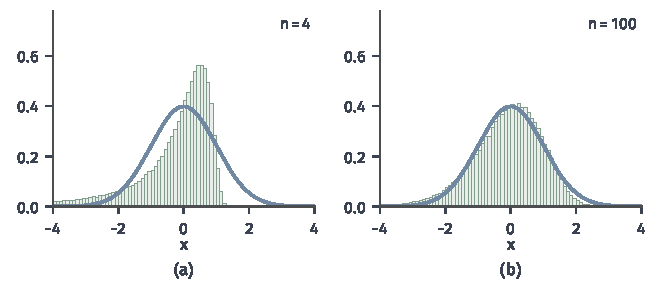
\includegraphics[width=112mm]{figures/07-probability/03-probability-limits/matplotlib/weak-slutsky/figure.pdf}
 \caption{Slutsky定理中的依赖分母。$X\sim\mathcal{N}(0,1)$，$X/(1+X/\sqrt n)$的直方图（浅绿，$2\times10^{5}$个样本，种子$3$，只画$[-4,4]$内的部分），蓝线为$\mathcal{N}(0,1)$的密度。(a)$n=4$，左侧的长尾来自分母接近零的样本；(b)$n=100$。}
 \label{fig:weak-slutsky}
\end{BookInlineFigure}

\paragraph{条件的作用}
常量分母必须非零。$X_n=Z\sim\mathcal{N}(0,1)$，$Y_n=1/n\xrightarrow{\mathbb{P}}0$，则$X_n/Y_n=nZ\sim\mathcal{N}(0,n^{2})$，质量逃向无穷远，没有弱极限。

常量也不能换成一般的随机极限。设$X_n=Z$，$Y_n=(-1)^{n}Z$，则$X_n\xrightarrow{\mathrm{d}}Z$，$Y_n\xrightarrow{\mathrm{d}}Z$，但
\[
 X_n+Y_n=\begin{cases}2Z,&n\text{为偶数},\\0,&n\text{为奇数}\end{cases}
\]
没有极限。两个分量各自依分布收敛到非退化的分布时，必须另外知道它们的联合收敛，例如由定理~\ref{thm:weak-independent-joint}的独立条件或由Cramér--Wold判据得到，才能谈论和的极限。


\section{分布积分的极限}
\label{sec:weak-integral-limits}

弱收敛控制的是有界连续函数的期望。可是最常用的量，均值、方差、高阶矩，都是无界函数的期望。设$X_n\xrightarrow{\mathrm{d}}X$，$g$连续而无界，$\mathbb{E}[g(X_n)]$是否趋于$\mathbb{E}[g(X)]$？

第~\ref{sec:weak-mass-control}节的例子给出否定的回答。$X_n$以概率$1/n$取$n$、否则取$0$。对$f\in C_b$，$\mathbb{E}[f(X_n)]=(1-1/n)f(0)+f(n)/n\to f(0)$，所以$X_n\xrightarrow{\mathrm{d}}0$。可是
\[
 \mathbb{E}[X_n]=n\cdot\frac1n=1\quad\text{对一切}n,\qquad\mathbb{E}[0]=0 .
\]
远处那份越来越轻的质量，乘以越来越大的位置，始终贡献$1$。弱收敛看不到它，因为有界函数在远处的读数被$\sup\lvert f\rvert/n$压住了；期望却要乘以位置本身。每个$X_n$的各阶矩都有限，$\mathbb{E}[X_n^{k}]=n^{k-1}$，但这对极限毫无帮助。

\paragraph{一致可积条件}
补上的条件正是第~\ref{sec:weak-mass-control}节对比过的一致可积：要求远处质量乘以位置之后，对所有$n$一致地小。

\begin{theorem}[期望的收敛]
\label{thm:weak-ui-expectation}
设$\bm{X}_n\xrightarrow{\mathrm{d}}\bm{X}$，$g:\mathbb{R}^{d}\to\mathbb{R}$可测，$\mathbb{P}(\bm{X}\in D_g)=0$，并且$\{g(\bm{X}_n)\}$一致可积：
\begin{equation}
 \lim_{r\to\infty}\sup_{n}\mathbb{E}\bigl[\lvert g(\bm{X}_n)\rvert\,\mathbf{1}_{\{\lvert g(\bm{X}_n)\rvert>r\}}\bigr]=0 .
 \label{eq:weak-ui}
\end{equation}
则$\mathbb{E}[\lvert g(\bm{X})\rvert]<\infty$，并且
\begin{equation}
 \lim_{n\to\infty}\mathbb{E}\bigl[g(\bm{X}_n)\bigr]=\mathbb{E}\bigl[g(\bm{X})\bigr] .
 \label{eq:weak-ui-expectation}
\end{equation}
\end{theorem}

\begin{proof}
记$Y_n=g(\bm{X}_n)$，$Y=g(\bm{X})$。由连续映射定理，$Y_n\xrightarrow{\mathrm{d}}Y$，于是问题化为实随机变量。对$r>0$，令截断函数
\[
 h_r(y)=\max\bigl(-r,\min(y,r)\bigr) ,
\]
它有界连续，与$y$只在$\lvert y\rvert>r$处不同，并且在那里与$y$之差的绝对值不超过$\lvert y\rvert$。

先证$Y$可积。$y\mapsto\min(\lvert y\rvert,r)$有界连续，所以
\[
 \mathbb{E}\bigl[\min(\lvert Y\rvert,r)\bigr]=\lim_{n\to\infty}\mathbb{E}\bigl[\min(\lvert Y_n\rvert,r)\bigr]\leq\sup_{n}\mathbb{E}\bigl[\lvert Y_n\rvert\bigr] .
\]
由式~\eqref{eq:weak-ui}，取$r_0$使尾部积分不超过$1$，则$\mathbb{E}[\lvert Y_n\rvert]\leq r_0+1$，右边有限。令$r\to\infty$，由单调收敛定理，$\mathbb{E}[\lvert Y\rvert]\leq r_0+1<\infty$。

再拆三项。对每个$r$，
\[
 \begin{aligned}
 \bigl\lvert\mathbb{E}[Y_n]-\mathbb{E}[Y]\bigr\rvert
 &\leq\mathbb{E}\bigl[\lvert Y_n\rvert\mathbf{1}_{\{\lvert Y_n\rvert>r\}}\bigr]+\bigl\lvert\mathbb{E}[h_r(Y_n)]-\mathbb{E}[h_r(Y)]\bigr\rvert\\
 &\quad+\mathbb{E}\bigl[\lvert Y\rvert\mathbf{1}_{\{\lvert Y\rvert>r\}}\bigr] .
 \end{aligned}
\]
任取$\varepsilon>0$。由式~\eqref{eq:weak-ui}，取$r$使第一项对一切$n$不超过$\varepsilon$；$Y$可积，由支配收敛定理，$r$足够大时第三项也不超过$\varepsilon$。固定这个$r$，令$n\to\infty$，第二项趋于零。于是左边的上极限不超过$2\varepsilon$。
\end{proof}

证明中“先证可积”这一步本身给出一个不需要一致可积的结论：只要$Y_n\xrightarrow{\mathrm{d}}Y$，就有
\begin{equation}
 \mathbb{E}\bigl[\lvert Y\rvert\bigr]\leq\liminf_{n\to\infty}\mathbb{E}\bigl[\lvert Y_n\rvert\bigr] .
 \label{eq:weak-fatou}
\end{equation}
推导时把$\sup_n$换成$\liminf_n$即可。它是Fatou引理在依分布收敛下的形式：极限只可能丢失期望，不会凭空增加。开头的例子中，$\mathbb{E}[X_n]=1$，极限的期望$0$严格变小，丢失的正是逃到远处的那一份。

一致可积常用矩条件验证。若存在$\delta>0$与常数$C$，使$\mathbb{E}[\lvert Y_n\rvert^{1+\delta}]\leq C$对一切$n$成立，则由于在$\lvert y\rvert>r$处$(\lvert y\rvert/r)^{\delta}>1$，
\[
 \sup_n\mathbb{E}\bigl[\lvert Y_n\rvert\mathbf{1}_{\{\lvert Y_n\rvert>r\}}\bigr]\leq\frac{C}{r^{\delta}}\longrightarrow0 .
\]
注意要的是比一阶稍高的矩的一致界；开头的例子中，每个$X_n$的高阶矩虽然有限，却没有一致界。

\paragraph{二项分布的矩}
$X_n\sim\operatorname{Bin}(n,2/n)\xrightarrow{\mathrm{d}}N\sim\operatorname{Poisson}(2)$。二阶矩是否收敛？可以直接计算：
\[
 \mathbb{E}[X_n^{2}]=\operatorname{Var}(X_n)+(\mathbb{E}[X_n])^{2}=2\Bigl(1-\frac2n\Bigr)+4=6-\frac4n\longrightarrow6=\mathbb{E}[N^{2}] .
\]
用定理~\ref{thm:weak-ui-expectation}也能得到，并且不需要精确的公式，只要一个三阶矩的界。

$X_n(X_n-1)(X_n-2)$等于从成功的试验中按顺序取出三个不同试验的方式数，每个有序三元组全部成功的概率为$p^{3}$，这里$p=2/n$，所以
\[
 \mathbb{E}[X_n(X_n-1)(X_n-2)]=n(n-1)(n-2)p^{3}\leq(np)^{3}=8 .
\]
同理$\mathbb{E}[X_n(X_n-1)]\leq(np)^{2}=4$。由$x^{3}=x(x-1)(x-2)+3x(x-1)+x$，
\[
 \mathbb{E}[X_n^{3}]\leq8+3\cdot4+2=22 .
\]
取$Y_n=X_n^{2}$，$\delta=1/2$，$\sup_n\mathbb{E}[\lvert Y_n\rvert^{3/2}]\leq22$，所以$\{X_n^{2}\}$一致可积，$\mathbb{E}[X_n^{2}]\to\mathbb{E}[N^{2}]$。同样的论证对任意阶矩都适用。图~\ref{fig:weak-ui-truncation}把这个例子与开头的反例并列。

\begin{BookInlineFigure}
 \centering
 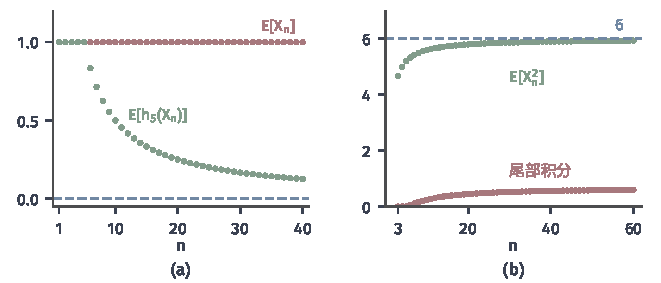
\includegraphics[width=112mm]{figures/07-probability/03-probability-limits/matplotlib/weak-ui-truncation/figure.pdf}
 \caption{期望能否随分布取极限。(a)$X_n$以概率$1/n$取$n$：$\mathbb{E}[X_n]$（红）恒为$1$，截断期望$\mathbb{E}[h_5(X_n)]$（绿）趋于极限的期望$0$（蓝色虚线），二者之差是$r=5$以外的尾部积分。(b)$X_n\sim\operatorname{Bin}(n,2/n)$：$\mathbb{E}[X_n^2]$（绿）趋于$6$（蓝色虚线），尾部积分$\mathbb{E}[X_n^2\mathbf{1}_{\{X_n^2>25\}}]$（红）对一切$n$都小于$0.7$，不随$n$增长。}
 \label{fig:weak-ui-truncation}
\end{BookInlineFigure}

\paragraph{与\texorpdfstring{$L^{1}$}{L1}收敛判据的区别}
第~\ref{chap:random-variable-convergence}章在同一概率空间上证明过：$X_n\xrightarrow{\mathbb{P}}X$且$\{X_n\}$一致可积，当且仅当$X_n\xrightarrow{L^{1}}X$，即$\mathbb{E}[\lvert X_n-X\rvert]\to0$。定理~\ref{thm:weak-ui-expectation}用的也是一致可积，但结论弱得多：它只说期望这一个数收敛，不涉及$\lvert X_n-X\rvert$，这个差可能根本没有定义。第~\ref{sec:weak-test-functions}节中$X(\omega)=\omega$、$X_n(\omega)=1-\omega$的例子里，期望恒等，而$\lvert1-2\omega\rvert$的平均$\mathbb{E}[\lvert X_n-X\rvert]=1/2$不趋于零。

\paragraph{不是期望的量}
定理处理的是固定函数$g$的期望。有些量由整个质量表或密度计算，不能写成某个固定$g$的期望，例如第~\ref{chap:information-measures}章的熵；弱收敛对它们没有一般的保证。格点均匀分布就是一例：$U_n$的质量表是$n$个$1/n$，任何只依赖各点质量大小的量都与$\operatorname{Unif}(0,1)$的密度无从比较，尽管$U_n\xrightarrow{\mathrm{d}}\operatorname{Unif}(0,1)$。这类量的极限要在相应的章节里另加条件讨论。


\section{本章小结}
\label{sec:weak-summary}

章首的两个例子，$\operatorname{Bin}(n,2/n)$趋于$\operatorname{Poisson}(2)$与格点均匀分布趋于$\operatorname{Unif}(0,1)$，现在都有了确切的含义：对每个有界连续函数，分布下的平均收敛。这个定义只比较分布，不要求随机变量在同一空间上，也不断言样本彼此接近；在共同空间上，依概率收敛推出依分布收敛，反之只在极限为常量时成立。有界保证读数存在，连续让质点位置的微小移动只引起读数的微小变化。

本章的工具按承担的任务可以分成几类，各有各的条件，见表~\ref{tab:weak-summary}。

\begin{BookInlineTable}
 \centering
 \caption{弱收敛的工具及其条件}
 \label{tab:weak-summary}
 \begin{tabular}{@{}lll@{}}
 \toprule
 任务 & 工具 & 关键条件\\
 \midrule
 事件概率 & Portmanteau定理 & 极限在事件边界上无质量\\
 实轴上的判据 & 分布函数判据 & 只在极限分布函数的连续点\\
 极限的存在 & 胎紧与弱收敛子列 & 远处质量一致地小\\
 极限的识别 & 特征函数唯一性 & 无\\
 收敛的判别 & 连续性定理 & 逐点极限在原点连续\\
 另一种表示 & 矩母函数 & 在$0$的邻域上有限\\
 映射的传递 & 连续映射定理 & 极限不在不连续点集上\\
 联合极限 & Cramér--Wold判据 & 检查所有方向的投影\\
 常量替换 & Slutsky定理 & 一个分量依概率趋于常量\\
 期望的极限 & 一致可积 & 远处质量乘位置一致地小\\
 \bottomrule
 \end{tabular}
\end{BookInlineTable}

几组容易混淆的区别值得再强调。胎紧控制远处有多少质量，一致可积还要乘上位置：前者决定极限分布是否存在，后者决定期望是否随之收敛。特征函数总存在，识别分布不需要任何条件；矩母函数只在零点邻域有限时才能识别，对数正态分布说明所有矩有限也不够。边缘收敛不推出联合收敛，坐标方向的投影也不能代替所有方向；只有一个分量的极限是常量时，配对问题才自动消失。

这些工具中，弱收敛的证明常常分两步完成：用胎紧或特征函数在原点的连续性保证质量不逃逸，再用特征函数的唯一性识别极限。下一章的中心极限定理正是这样证明的：把标准化和的特征函数写成乘积，用二阶展开和乘积之差的引理求出高斯极限，再由连续性定理得到依分布收敛；多元情形则用Cramér--Wold判据化为各个方向。之后各章比较分布的距离时，也直接沿用本章的弱收敛，不再重新建立。


\chapter{中心极限定理}
\label{chap:central-limit-theorem}

把一枚均匀硬币掷$100$次，正面次数$S$的平均是$50$。大数律告诉我们，正面比例$S/100$会随掷的次数增多而靠近$1/2$；可是在$100$次这个具体的规模上，$S$不超过$55$的机会有多大？二项分布是已知的，把$56$个质量加起来，得到约$0.8644$。换一种算法：$S$的标准差是$5$，$55$比均值高出一个标准差，标准高斯分布在$1$处的分布函数值是$0.8413$；若把阈值取在$55.5$，得到$0.8643$，几乎与精确值重合。

钟形曲线为什么会出现在这里？硬币的每一次结果只取$0$和$1$，没有一点钟形的样子。原因在于$S$是$100$个独立小项之和：每一项单独都很粗糙，加起来以后，它们的细节互相抵消，留下的只有均值和方差。这就是\term{中心极限定理}（central limit theorem）所描述的现象：许多独立小扰动之和，中心化并按标准差缩放以后，分布逼近标准高斯分布。

这一章回答三个问题。第一，应当在什么尺度上观察波动：大数律说平均的偏差趋于零，偏差本身要放大多少倍才有稳定的形状。第二，什么条件保证放大后的形状是高斯的：独立同分布、各项分布不同、取值为向量，条件各有不同。第三，有限的样本量下，用高斯分布代替真实分布的误差有多大，又在哪些问题上不能这样代替。

全章以掷硬币的正面次数为主要例子，以指数分布的等待时间作为偏斜的对照。先确定标准化的中心和尺度，再在独立同分布情形用特征函数证明定理，然后放宽到三角阵和随机向量，最后用Berry--Esseen界估计正态近似的误差，并说明这个界管不到的地方。所用的弱收敛、特征函数及其连续性定理、Cramér--Wold判据都来自第~\ref{chap:weak-convergence-of-distributions}章。

\section{标准化波动}
\label{sec:clt-standardized}

掷$n$次硬币，我们可以看正面次数$S_n$，也可以看正面比例$\bar{X}_n=S_n/n$。两者只差一个因子$n$，可是随着$n$增大，一个越来越分散，一个越来越集中。要谈“波动的形状”，先得说清楚三件事：以什么为中心，看哪一个误差量，把误差放大多少倍。

第~\ref{chap:laws-of-large-numbers}章的大数律回答了中心的问题：样本平均趋于总体均值$\mu$，平均的偏差$\bar{X}_n-\mu$趋于零。它没有回答偏差以多快的速度缩小，也没有说明把偏差放大到合适的倍数以后是什么样子。本节先用方差确定合适的放大倍数，再说明标准化能做到什么、做不到什么。

\subsection{部分和与平均的尺度}
\label{sec:clt-scales}

设$X_1,X_2,\dots$独立同分布，均值为$\mu$，方差$\sigma^2$有限且大于零。记部分和与样本平均为
\[
 S_n=X_1+\dots+X_n,\qquad \bar{X}_n=\frac{S_n}{n} .
\]
两种误差量分别是部分和偏离$n\mu$的量$S_n-n\mu$，以及平均偏离$\mu$的量$\bar{X}_n-\mu$。

\paragraph{两种误差的方差}
独立随机变量之和的方差等于方差之和，常数平移不改变方差，所以
\[
 \operatorname{Var}(S_n-n\mu)=\sum_{i=1}^{n}\operatorname{Var}(X_i)=n\sigma^2 .
\]
再利用$\operatorname{Var}(aY)=a^2\operatorname{Var}(Y)$，取$a=1/n$，得到
\[
 \operatorname{Var}(\bar{X}_n-\mu)=\frac{1}{n^2}\cdot n\sigma^2=\frac{\sigma^2}{n} .
\]
两个结果合起来，标准差分别是
\begin{equation}
 \sqrt{\operatorname{Var}(S_n-n\mu)}=\sigma\sqrt{n},\qquad
 \sqrt{\operatorname{Var}(\bar{X}_n-\mu)}=\frac{\sigma}{\sqrt{n}} .
 \label{eq:clt-scales}
\end{equation}

部分和的典型偏差随$\sqrt{n}$增长，比$n$慢；平均的典型偏差随$1/\sqrt{n}$缩小，比$1/n$慢。前者慢于$n$，是因为独立的正负偏差互相抵消了一部分；后者慢于$1/n$，原因相同。把$n$项完全同向的偏差相加，标准差才会是$n\sigma$。

\paragraph{掷硬币}
设$X_i\sim\operatorname{Bern}(1/2)$，则$\mu=1/2$，$\sigma^2=1/4$，$S_n\sim\operatorname{Bin}(n,1/2)$。由式~\eqref{eq:clt-scales}，次数与比例的标准差分别为$\sqrt{n}/2$与$1/(2\sqrt{n})$。取$n=10,40,160$，
\[
 \frac{\sqrt{n}}{2}\approx1.58,\ 3.16,\ 6.32;\qquad \frac{1}{2\sqrt{n}}\approx0.158,\ 0.079,\ 0.040 .
\]
$n$每变成四倍，次数的标准差加倍，比例的标准差减半。

图~\ref{fig:clt-binomial-scales}画出这三个$n$下的精确质量表。左图以$n/2$为中心看次数，质量表随$n$摊开，峰值下降；右图以$1/2$为中心看比例，质量表向中心收拢。为了让不同$n$可比，右图的纵轴是质量除以格点间距$1/n$，这样曲线下的面积都是一。

\begin{BookInlineFigure}
 \centering
 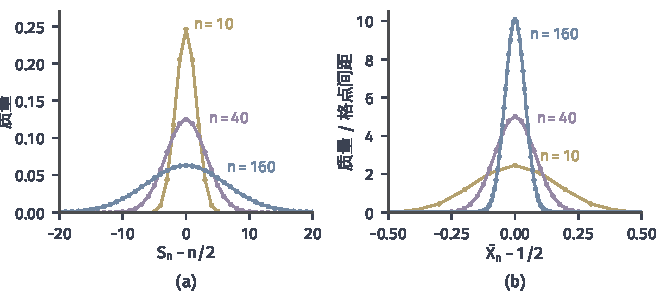
\includegraphics[width=112mm]{figures/07-probability/03-probability-limits/matplotlib/clt-binomial-scales/figure.pdf}
 \caption{均匀硬币掷$n$次的正面次数$S_n\sim\operatorname{Bin}(n,1/2)$，$n=10$（黄）、$40$（紫）、$160$（蓝），折线连接各格点上的精确质量。(a)中心化次数$S_n-n/2$的质量，宽度按$\sqrt{n}/2$增长；(b)中心化比例$\bar{X}_n-1/2$的质量除以格点间距$1/n$，宽度按$1/(2\sqrt{n})$缩小。}
 \label{fig:clt-binomial-scales}
\end{BookInlineFigure}

\paragraph{两种尺度不能混用}
这两个量回答不同的问题。问“正面次数偏离$n/2$不超过$5$次的概率”，随着$n$增大，这个概率趋于零，因为次数的典型偏差$\sqrt{n}/2$终将远超$5$。问“正面比例偏离$1/2$不超过$0.05$的概率”，它趋于一，这是大数律。两句话都对，只是固定的容许量$5$与$0.05$放在了不同的尺度上。

\paragraph{放大的倍数}
要得到不随$n$消失、也不随$n$发散的波动，可以把平均的偏差乘以$n^{a}$，看哪个$a$合适。由$\operatorname{Var}(cY)=c^2\operatorname{Var}(Y)$，
\[
 \operatorname{Var}\bigl(n^{a}(\bar{X}_n-\mu)\bigr)=n^{2a}\cdot\frac{\sigma^2}{n}=n^{2a-1}\sigma^2 .
\]
$a<1/2$时方差趋于零，由Chebyshev不等式，对每个$t>0$，
\[
 \mathbb{P}\bigl(\lvert n^{a}(\bar{X}_n-\mu)\rvert\geq t\bigr)\leq\frac{n^{2a-1}\sigma^2}{t^2}\to0 ,
\]
放大后的偏差依概率趋于零，形状缩成一点。$a>1/2$时方差趋于无穷，偏差越放越大。只有$a=1/2$时方差恒为$\sigma^2$。

图~\ref{fig:clt-three-scalings}用掷硬币的精确分布画出$a=0.3,0.5,0.7$三种放大下，中间$90\%$质量所在的区间随$n$的变化。三幅图的区间分别收窄、保持、扩张，紫色虚线是按方差预测的$\pm1.645\cdot\frac12 n^{a-1/2}$，其中$1.645$是标准高斯分布的$95\%$分位数。$a=1/2$时区间端点稳定在$\pm0.82$附近，与这条虚线吻合，这已经在提示极限分布是高斯的。

\begin{BookInlineFigure}
 \centering
 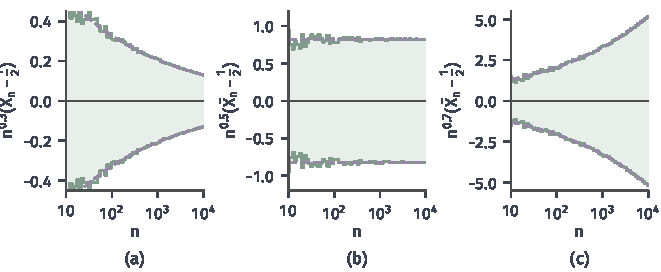
\includegraphics[width=112mm]{figures/07-probability/03-probability-limits/matplotlib/clt-three-scalings/figure.pdf}
 \caption{掷硬币时$n^{a}(\bar{X}_n-1/2)$的$5\%$与$95\%$分位数（绿色阶梯，由$\operatorname{Bin}(n,1/2)$精确计算），$n$从$10$到$10^{4}$，横轴为对数刻度。(a)$a=0.3$；(b)$a=0.5$；(c)$a=0.7$。紫色虚线为$\pm1.645\cdot\frac12n^{a-1/2}$。}
 \label{fig:clt-three-scalings}
\end{BookInlineFigure}

\paragraph{大数律与中心极限的分工}
大数律相当于取$a=0$：平均的偏差本身趋于零，它确定了极限的位置。中心极限定理研究$a=1/2$时放大后偏差的分布。前者不能推出后者：知道偏差趋于零，并不知道它以$1/\sqrt{n}$的速度趋于零，更不知道放大以后呈什么形状。下一小节会看到，平均同样趋于中心，放大后的形状却可以不是钟形。

方差无穷时，式~\eqref{eq:clt-scales}失去意义。例如第~\ref{chap:tail-probabilities}章参数为$3/2$的Pareto分布，均值有限，样本平均仍满足大数律，方差却是无穷，$\sqrt{n}$不再是合适的放大倍数。本章始终假设方差有限，这类重尾的极限需要别的尺度，不在本卷讨论。

\subsection{标准化的选择}
\label{sec:clt-standardization}

确定了放大倍数$\sqrt{n}$，再除以单项的标准差，就把波动的单位也去掉了。由式~\eqref{eq:clt-scales}，中心化部分和除以它自己的标准差，与平均的偏差乘$\sqrt{n}$再除以$\sigma$，是同一个量。

\begin{definition}[标准化部分和]
\label{def:clt-standardized-sum}
设$X_1,\dots,X_n$独立同分布，均值为$\mu$，方差$\sigma^2\in(0,\infty)$。称
\begin{equation}
 Z_n=\frac{S_n-n\mu}{\sigma\sqrt{n}}=\frac{\sqrt{n}\,(\bar{X}_n-\mu)}{\sigma}
 \label{eq:clt-zn}
\end{equation}
为标准化部分和。
\end{definition}

$Z_n$正是第~\ref{chap:random-variable-moments}章意义下$S_n$的标准化，也是$\bar{X}_n$的标准化：两者只差一个正的倍数，标准化后相同。由式~\eqref{eq:clt-scales}，对每个$n$都有
\[
 \mathbb{E}[Z_n]=0,\qquad \operatorname{Var}(Z_n)=1 .
\]
掷硬币时$\mu=1/2$，$\sigma=1/2$，于是$Z_n=(2S_n-n)/\sqrt{n}$。$n=100$时$Z_{100}=(S_{100}-50)/5$，章首的阈值$55$对应$Z_{100}=1$。

\paragraph{方差为一不等于钟形}
标准化只做平移和正的缩放，不改变分布的形状。$n=1$时$Z_1$就是$X_1$的标准化，硬币的$Z_1$只取$\pm1$两个值，与钟形毫无关系。$Z_n$接近钟形，是因为$S_n$是许多独立项之和，不是因为除以了标准差。

即使项数很多，标准化也不能保证钟形。设第$n$次试验掷$n$枚特制的硬币，每枚正面的概率是$1/n$，正面总数$S_n\sim\operatorname{Bin}(n,1/n)$。它的均值和方差是
\[
 \mathbb{E}[S_n]=1,\qquad \operatorname{Var}(S_n)=n\cdot\frac1n\Bigl(1-\frac1n\Bigr)=1-\frac1n .
\]
平均$S_n/n$同样趋于零，标准化以后均值为零、方差为一。可是$S_n$只取非负整数，它的前几个质量趋于
\[
 \mathbb{P}(S_n=0)=\Bigl(1-\frac1n\Bigr)^{n}\to\mathrm{e}^{-1}\approx0.368,\qquad
 \mathbb{P}(S_n=1)=\Bigl(1-\frac1n\Bigr)^{n-1}\to\mathrm{e}^{-1} .
\]
一般地，第~\ref{chap:common-distributions}章已经说明$\operatorname{Bin}(n,\lambda/n)$的质量趋于$\operatorname{Poisson}(\lambda)$的质量，这里$\lambda=1$，所以$S_n-1$的分布逼近$\operatorname{Poisson}(1)$平移$-1$后的分布。

图~\ref{fig:clt-poisson-counter}把这两种标准化计数放在一起。左边是$\operatorname{Bin}(100,1/2)$，格点间距$1/5$，质量除以间距后贴着标准高斯密度$\varphi$；右边是$\operatorname{Bin}(100,1/100)$，标准化以后只有几根竖线，集中在$z=-1,0,1,2$附近，没有平滑的钟形。

\begin{BookInlineFigure}
 \centering
 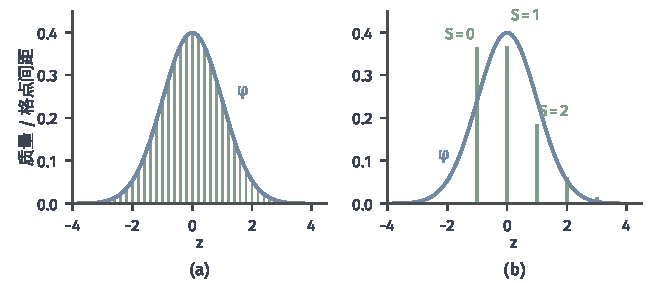
\includegraphics[width=112mm]{figures/07-probability/03-probability-limits/matplotlib/clt-poisson-counter/figure.pdf}
 \caption{两个$n=100$的标准化二项计数，均值都为$0$、方差都为$1$。绿色竖线是精确质量除以格点间距$1/\sigma_n$，蓝线是标准高斯密度$\varphi$。(a)$\operatorname{Bin}(100,1/2)$，$\sigma_n=5$；(b)$\operatorname{Bin}(100,1/100)$，$\sigma_n\approx0.995$，质量集中在$S=0,1,2$等少数格点。}
 \label{fig:clt-poisson-counter}
\end{BookInlineFigure}

两种计数的差别在于每一项对总和的影响。正面概率为$1/2$时，每枚硬币只贡献总方差的$1/n$，没有哪一枚举足轻重；正面概率为$1/n$时，总和几乎由“偶尔出现的一次正面”决定，这样一次正面就让$S_n$跳动一个标准差。第~\ref{sec:clt-non-identical}节会把“没有一项举足轻重”写成可以核验的条件。

\paragraph{零方差}
定义~\ref{def:clt-standardized-sum}要求$\sigma^2>0$。若$\sigma^2=0$，则$X_i$以概率一等于$\mu$，部分和$S_n-n\mu$以概率一为零，没有波动可言，也不能除以$\sigma$。此时不作标准化，直接说$\sqrt{n}(\bar{X}_n-\mu)$以概率一等于零，它的分布是$0$处的单点分布。把方差为零的高斯分布$\mathcal{N}(0,0)$理解为这个单点分布，零方差情形也可以纳入第~\ref{sec:clt-multivariate}节的统一陈述。


\section{独立同分布情形}
\label{sec:clt-iid}

标准化部分和$Z_n$的均值和方差已经固定为$0$和$1$，上一节也看到，形状要靠“许多独立的小项”才会变成钟形。最简单的情形是各项来自同一个分布：每一项对总和的贡献都是总方差的$1/n$，没有哪一项占优。本节在这个情形下陈述并证明中心极限定理，只要求方差有限。

\subsection{定理与条件}
\label{sec:clt-iid-theorem}

先看一个偏斜得很厉害的例子。设$X_i\sim\operatorname{Exp}(1)$独立，表示一串相互独立的等待时间，$\mu=\sigma=1$。由第~\ref{chap:random-variable-transformations}章的卷积计算，$S_n\sim\operatorname{Gamma}(n,1)$，所以$Z_n=(S_n-n)/\sqrt{n}$的密度可以精确写出：
\[
 f_{Z_n}(z)=\sqrt{n}\,f_{S_n}(n+z\sqrt{n}),\qquad f_{S_n}(s)=\frac{s^{n-1}\mathrm{e}^{-s}}{(n-1)!}\ (s>0) .
\]
这里用了第~\ref{chap:random-variable-transformations}章的一元换元：$Z_n$是$S_n$的仿射函数，密度要乘以斜率的倒数$\sqrt{n}$。

图~\ref{fig:clt-gamma-densities}画出$n=1,4,16$时的$f_{Z_n}$。$n=1$时它是平移后的指数密度，在$z=-1$处突然跳起，右侧拖着长尾；$n=4$时已经有了圆顶，但峰偏在左边；$n=16$时与标准高斯密度只差一点偏斜。偏斜的程度可以用偏度衡量，$\operatorname{Gamma}(n,1)$的偏度是$2/\sqrt{n}$，按$1/\sqrt{n}$消失。

\begin{BookInlineFigure}
 \centering
 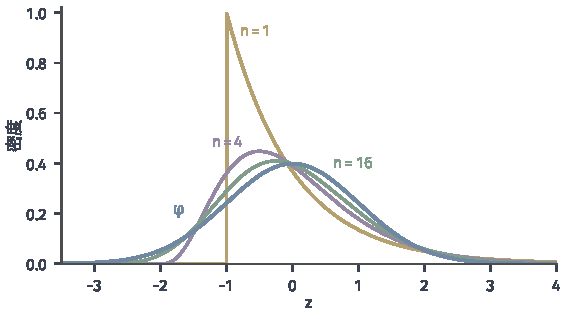
\includegraphics[width=96mm]{figures/07-probability/03-probability-limits/matplotlib/clt-gamma-densities/figure.pdf}
 \caption{$n$个独立$\operatorname{Exp}(1)$之和的标准化$Z_n=(S_n-n)/\sqrt{n}$的精确密度，$n=1$（黄）、$4$（紫）、$16$（绿），蓝线为标准高斯密度$\varphi$。$n=1$时密度在$z=-1$处从$0$跳到$1$。}
 \label{fig:clt-gamma-densities}
\end{BookInlineFigure}

硬币与等待时间的单项分布截然不同，一个只取两个值，一个是连续的偏斜密度，标准化和却都趋于同一个形状。下面的定理说，只要独立、同分布、方差有限且为正，这个现象总会发生。

\begin{theorem}[独立同分布的中心极限定理]
\label{thm:clt-iid}
设$X_1,X_2,\dots$独立同分布，$\mathbb{E}[X_1]=\mu$，$\operatorname{Var}(X_1)=\sigma^2\in(0,\infty)$，$Z_n$如式~\eqref{eq:clt-zn}。则
\begin{equation}
 Z_n=\frac{S_n-n\mu}{\sigma\sqrt{n}}\xrightarrow{\mathrm{d}}\mathcal{N}(0,1) .
 \label{eq:clt-iid}
\end{equation}
\end{theorem}

\paragraph{用分布函数表述}
标准高斯分布函数$\Phi$处处连续，没有需要排除的跳点。由第~\ref{chap:weak-convergence-of-distributions}章的分布函数判据，式~\eqref{eq:clt-iid}等价于对每个实数$x$，
\begin{equation}
 \mathbb{P}(Z_n\leq x)\to\Phi(x) .
 \label{eq:clt-iid-cdf}
\end{equation}
于是对任意$a<b$，$\mathbb{P}(a<Z_n\leq b)\to\Phi(b)-\Phi(a)$。端点是否取等号不影响极限：$\mathbb{P}(Z_n=x)\leq\mathbb{P}(x-\eta<Z_n\leq x)$对每个$\eta>0$成立，右边趋于$\Phi(x)-\Phi(x-\eta)$，可以任意小。

把定理用于$X_i\sim\operatorname{Bern}(p)$，$0<p<1$，就得到二项计数的正态逼近：
\[
 \frac{S_n-np}{\sqrt{np(1-p)}}\xrightarrow{\mathrm{d}}\mathcal{N}(0,1),\qquad S_n\sim\operatorname{Bin}(n,p) .
\]
这个特例称为\term{de Moivre--Laplace定理}（de Moivre--Laplace theorem），它是中心极限定理最早的形式。

\paragraph{各个条件的作用}
定理有三个条件。独立性使和的特征函数能拆成乘积，这是证明的起点；同分布使每个因子相同，$n$个小贡献完全对称；方差有限且为正，既给出了标准化的尺度，也保证下面的二阶展开成立。上一节的特制硬币各项分布随$n$变化，不在定理的范围里，它的极限也确实不是高斯的。

定理只要求二阶矩有限，不要求三阶矩，也不要求矩母函数存在。第~\ref{sec:clt-error}节估计近似误差时要用三阶绝对矩，那是为了得到收敛的速度，不是收敛本身的条件。第~\ref{chap:weak-convergence-of-distributions}章说明过，矩母函数可能在零点附近的任何邻域都无穷，而特征函数总是存在，所以证明用特征函数。

\subsection{特征函数证明}
\label{sec:clt-iid-proof}

把$X_i$标准化，令$Y_i=(X_i-\mu)/\sigma$。$Y_i$独立同分布，$\mathbb{E}[Y_i]=0$，$\mathbb{E}[Y_i^2]=1$，并且
\[
 Z_n=\frac{1}{\sqrt{n}}\sum_{i=1}^{n}Y_i .
\]
记$Y$为与$Y_i$同分布的变量，$\phi_Y$为它的特征函数。第~\ref{chap:weak-convergence-of-distributions}章给出了两条运算规则：数乘满足$\phi_{cY}(t)=\phi_Y(ct)$；独立变量之和的特征函数是各自特征函数的乘积。合起来，
\begin{equation}
 \phi_{Z_n}(t)=\prod_{i=1}^{n}\phi_{Y_i}\Bigl(\frac{t}{\sqrt{n}}\Bigr)=\phi_Y\Bigl(\frac{t}{\sqrt{n}}\Bigr)^{n} .
 \label{eq:clt-product}
\end{equation}
标准高斯分布的特征函数是$\mathrm{e}^{-t^2/2}$，由连续性定理，只需证明式~\eqref{eq:clt-product}对每个$t$趋于$\mathrm{e}^{-t^2/2}$。

\paragraph{为什么会出现$\mathrm{e}^{-t^2/2}$}
先用直觉看一遍。$t/\sqrt{n}$很小，$\phi_Y$在原点附近的展开是
\[
 \phi_Y(s)=\mathbb{E}[\mathrm{e}^{\mathrm{i}sY}]\approx1+\mathrm{i}s\,\mathbb{E}[Y]-\frac{s^2}{2}\mathbb{E}[Y^2]=1-\frac{s^2}{2} .
\]
代入$s=t/\sqrt{n}$再取$n$次方，
\[
 \phi_{Z_n}(t)\approx\Bigl(1-\frac{t^2}{2n}\Bigr)^{n}\to\mathrm{e}^{-t^2/2} .
\]
中心化让一次项消失，方差为一让二次项的系数是$1/2$。剩下要说明的是：被“$\approx$”丢掉的余项乘上$n$个因子以后，累计起来仍然可以忽略。

第~\ref{chap:weak-convergence-of-distributions}章在二阶矩有限时给出了上面的展开，余项是$s^2$的高阶无穷小。为了在$n$个因子的乘积里累计余项，我们把余项写成显式的界，下面两个引理分别处理单个因子和乘积。

\begin{lemma}[复指数的二阶展开]
\label{lem:clt-exp-remainder}
对每个实数$x$，
\begin{equation}
 \Bigl\lvert\mathrm{e}^{\mathrm{i}x}-1-\mathrm{i}x+\frac{x^2}{2}\Bigr\rvert\leq\min\Bigl\{\frac{\lvert x\rvert^{3}}{6},\ x^2\Bigr\} .
 \label{eq:clt-exp-remainder}
\end{equation}
\end{lemma}

\begin{proof}
对积分$\int_0^x(x-u)\mathrm{e}^{\mathrm{i}u}\,\mathrm{d}u$分部积分，取$\mathrm{e}^{\mathrm{i}u}$的原函数$-\mathrm{i}\mathrm{e}^{\mathrm{i}u}$，得到
\[
 \int_0^x(x-u)\mathrm{e}^{\mathrm{i}u}\,\mathrm{d}u
 =\Bigl[-\mathrm{i}(x-u)\mathrm{e}^{\mathrm{i}u}\Bigr]_0^x-\mathrm{i}\int_0^x\mathrm{e}^{\mathrm{i}u}\,\mathrm{d}u
 =\mathrm{i}x-(\mathrm{e}^{\mathrm{i}x}-1) .
\]
移项得到一次展开的余项公式
\[
 \mathrm{e}^{\mathrm{i}x}-1-\mathrm{i}x=-\int_0^x(x-u)\mathrm{e}^{\mathrm{i}u}\,\mathrm{d}u .
\]

第一个界。$x^2/2=\int_0^x(x-u)\,\mathrm{d}u$，与上式相加，
\[
 \mathrm{e}^{\mathrm{i}x}-1-\mathrm{i}x+\frac{x^2}{2}=\int_0^x(x-u)\bigl(1-\mathrm{e}^{\mathrm{i}u}\bigr)\,\mathrm{d}u .
\]
被积函数中$\lvert1-\mathrm{e}^{\mathrm{i}u}\rvert\leq2$，$x-u$在积分区间上不变号，所以
\[
 \Bigl\lvert\mathrm{e}^{\mathrm{i}x}-1-\mathrm{i}x+\frac{x^2}{2}\Bigr\rvert\leq2\Bigl\lvert\int_0^x(x-u)\,\mathrm{d}u\Bigr\rvert=x^2 .
\]

第二个界。再对$\int_0^x(x-u)^2\mathrm{e}^{\mathrm{i}u}\,\mathrm{d}u$分部积分，并代入前面的结果：
\[
 \int_0^x(x-u)^2\mathrm{e}^{\mathrm{i}u}\,\mathrm{d}u
 =\mathrm{i}x^2-2\mathrm{i}\int_0^x(x-u)\mathrm{e}^{\mathrm{i}u}\,\mathrm{d}u
 =\mathrm{i}x^2-2\mathrm{i}\bigl(1+\mathrm{i}x-\mathrm{e}^{\mathrm{i}x}\bigr) .
\]
两边除以$2\mathrm{i}$并整理，
\[
 \mathrm{e}^{\mathrm{i}x}-1-\mathrm{i}x+\frac{x^2}{2}=\frac{1}{2\mathrm{i}}\int_0^x(x-u)^2\mathrm{e}^{\mathrm{i}u}\,\mathrm{d}u .
\]
被积函数的模是$(x-u)^2$，所以
\[
 \Bigl\lvert\mathrm{e}^{\mathrm{i}x}-1-\mathrm{i}x+\frac{x^2}{2}\Bigr\rvert\leq\frac12\Bigl\lvert\int_0^x(x-u)^2\,\mathrm{d}u\Bigr\rvert=\frac{\lvert x\rvert^3}{6} .
\]
\end{proof}

两个界各管一段，见图~\ref{fig:clt-remainder}。$\lvert x\rvert$小的时候，三次界$\lvert x\rvert^3/6$更小，余项确实是三阶小量；$\lvert x\rvert$大的时候，二次界$x^2$更小，因为余项最多和$x^2/2$同阶，不会像$\lvert x\rvert^3$那样增长。两条界在$\lvert x\rvert=6$处相交。证明中正是要用后一个界：$Y$只有二阶矩，$\mathbb{E}[\lvert Y\rvert^3]$可能是无穷，但$\mathbb{E}[Y^2]$一定有限。

\begin{BookInlineFigure}
 \centering
 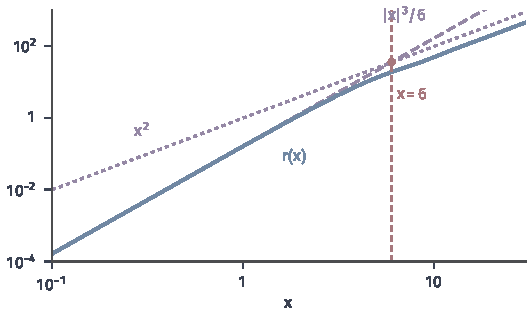
\includegraphics[width=90mm]{figures/07-probability/03-probability-limits/matplotlib/clt-remainder/figure.pdf}
 \caption{二阶展开的余项$r(x)=\lvert\mathrm{e}^{\mathrm{i}x}-1-\mathrm{i}x+x^2/2\rvert$（蓝）与两条上界$\lvert x\rvert^3/6$（紫色虚线）、$x^2$（紫色点线），双对数坐标。两条界在$x=6$（红点）相交，$x<6$时三次界更紧，$x>6$时二次界更紧。}
 \label{fig:clt-remainder}
\end{BookInlineFigure}

\begin{lemma}[乘积之差]
\label{lem:clt-product-difference}
设复数$z_1,\dots,z_m$与$w_1,\dots,w_m$的模都不超过$1$。则
\begin{equation}
 \Bigl\lvert\prod_{k=1}^{m}z_k-\prod_{k=1}^{m}w_k\Bigr\rvert\leq\sum_{k=1}^{m}\lvert z_k-w_k\rvert .
 \label{eq:clt-product-difference}
\end{equation}
\end{lemma}

\begin{proof}
对$m$归纳。$m=1$时两边相等。设结论对$m-1$成立，记$P=\prod_{k<m}z_k$，$Q=\prod_{k<m}w_k$，它们的模不超过$1$。拆开差，
\[
 Pz_m-Qw_m=z_m(P-Q)+(z_m-w_m)Q .
\]
由$\lvert z_m\rvert\leq1$与$\lvert Q\rvert\leq1$，
\[
 \lvert Pz_m-Qw_m\rvert\leq\lvert P-Q\rvert+\lvert z_m-w_m\rvert ,
\]
再对$\lvert P-Q\rvert$用归纳假设即得。
\end{proof}

这个引理说，模不超过一的因子相乘时，各因子的误差至多简单相加，不会被放大。所以只要每个因子的误差是$o(1/n)$，$n$个因子的累计误差就是$o(1)$。

\begin{proof}[定理~\ref{thm:clt-iid}的证明]
固定$t$，记$s=t/\sqrt{n}$。

第一步，单个因子的误差。在式~\eqref{eq:clt-exp-remainder}中令$x=sY$，取期望。由$\mathbb{E}[Y]=0$，$\mathbb{E}[Y^2]=1$，左边期望里的各项分别给出$\phi_Y(s)$、$1$、$0$和$s^2/2$；再用“期望的模不超过模的期望”，得到
\[
 \Bigl\lvert\phi_Y(s)-\Bigl(1-\frac{s^2}{2}\Bigr)\Bigr\rvert
 \leq\mathbb{E}\Bigl[\min\Bigl\{\frac{\lvert s\rvert^{3}\lvert Y\rvert^{3}}{6},\ s^2Y^2\Bigr\}\Bigr] .
\]
代入$s=t/\sqrt{n}$，两边乘$n$，
\[
 n\Bigl\lvert\phi_Y\Bigl(\frac{t}{\sqrt{n}}\Bigr)-\Bigl(1-\frac{t^2}{2n}\Bigr)\Bigr\rvert
 \leq t^2\,\mathbb{E}\Bigl[\min\Bigl\{\frac{\lvert t\rvert\,\lvert Y\rvert^{3}}{6\sqrt{n}},\ Y^2\Bigr\}\Bigr] .
\]

第二步，右边趋于零。期望里的随机变量对每个样本点都趋于零，因为$\lvert Y\rvert^3/\sqrt{n}\to0$；它又被可积的$Y^2$控制。由支配收敛定理，右边的期望趋于零。这里只用到$\mathbb{E}[Y^2]<\infty$。

第三步，累计。$n\geq t^2/2$时，$\lvert1-t^2/(2n)\rvert\leq1$；特征函数的模也不超过$1$。对式~\eqref{eq:clt-product}的$n$个因子用引理~\ref{lem:clt-product-difference}，
\[
 \Bigl\lvert\phi_{Z_n}(t)-\Bigl(1-\frac{t^2}{2n}\Bigr)^{n}\Bigr\rvert
 \leq n\Bigl\lvert\phi_Y\Bigl(\frac{t}{\sqrt{n}}\Bigr)-\Bigl(1-\frac{t^2}{2n}\Bigr)\Bigr\rvert\to0 .
\]

第四步，极限。由$\ln(1-y)/y\to-1$（$y\to0$），$n\ln(1-t^2/(2n))\to-t^2/2$，所以
\[
 \Bigl(1-\frac{t^2}{2n}\Bigr)^{n}\to\mathrm{e}^{-t^2/2} .
\]
两步合起来，$\phi_{Z_n}(t)\to\mathrm{e}^{-t^2/2}$对每个$t$成立。极限是$\mathcal{N}(0,1)$的特征函数，由连续性定理，$Z_n\xrightarrow{\mathrm{d}}\mathcal{N}(0,1)$。
\end{proof}

图~\ref{fig:clt-proof-flow}把证明的链条和每一环所用的条件放在一起。独立性只在第一个方框用到；中心化和方差为一决定展开式的形状；二阶矩有限只在支配收敛那一步用到；最后由连续性定理从特征函数回到分布。

\begin{BookInlineFigure}
 \centering
 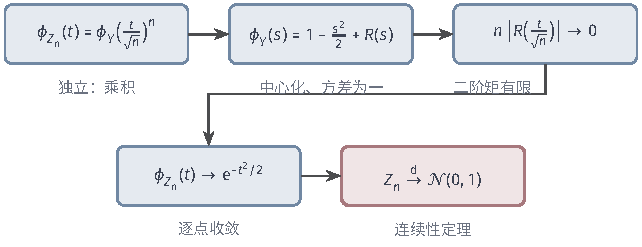
\includegraphics[width=109mm]{figures/07-probability/03-probability-limits/tikz/clt-proof-flow/figure.pdf}
 \caption{中心极限定理的特征函数证明。方框是各步得到的结论，框下灰字是该步所用的条件或工具，红框是要证明的依分布收敛。}
 \label{fig:clt-proof-flow}
\end{BookInlineFigure}

\paragraph{去掉中心化会怎样}
若不减去$\mu$，直接看$S_n/(\sigma\sqrt{n})$，它的特征函数多出因子$\mathrm{e}^{\mathrm{i}t\sqrt{n}\mu/\sigma}$。$\mu\neq0$时这个因子绕单位圆越转越快，对$t\neq0$没有极限，分布的位置以$\sqrt{n}$的速度跑向无穷。中心化就是把这个漂移去掉。

\paragraph{硬币的特征函数}
用硬币核对一遍。把一次结果写成$Y=2X-1$，以各$1/2$的概率取$\pm1$，它已经中心化且方差为一。它的特征函数是
\[
 \phi_Y(s)=\tfrac12\mathrm{e}^{\mathrm{i}s}+\tfrac12\mathrm{e}^{-\mathrm{i}s}=\cos s .
\]
由式~\eqref{eq:clt-product}，$\phi_{Z_n}(t)=\cos(t/\sqrt{n})^{n}$。取$t=1$，$n=1,4,16$时依次为
\[
 \cos1\approx0.5403,\qquad \cos(0.5)^{4}\approx0.5931,\qquad \cos(0.25)^{16}\approx0.6033 ,
\]
极限值是$\mathrm{e}^{-1/2}\approx0.6065$。$n=16$时，近似式$(1-t^2/(2n))^n=(1-1/32)^{16}\approx0.6017$也已接近极限。

证明中的几个量也可以在这里逐一算出。$n=16$、$t=1$时$s=1/4$，单个因子的误差是
\[
 \Bigl\lvert\cos\frac14-\Bigl(1-\frac{1}{32}\Bigr)\Bigr\rvert\approx\lvert0.968912-0.968750\rvert\approx1.62\times10^{-4} ,
\]
乘以$n=16$得到约$2.6\times10^{-3}$。第三步说两个乘积之差不超过这个数，实际的差是
\[
 \lvert0.6033-0.6017\rvert\approx1.6\times10^{-3} .
\]
第一步的上界中$\lvert Y\rvert=1$，它给出
\[
 t^2\,\mathbb{E}\Bigl[\min\Bigl\{\frac{\lvert t\rvert\,\lvert Y\rvert^{3}}{6\sqrt{n}},\ Y^2\Bigr\}\Bigr]=\frac{1}{24}\approx0.042 ,
\]
比实际误差大得多。原因是硬币对称，$\mathbb{E}[Y^3]=0$，$\cos s$的展开中没有三次项，误差从四次项$s^4/24$开始；引理~\ref{lem:clt-exp-remainder}不知道这种对称性，只能按三次估计。证明只需要误差趋于零，不需要它紧。

图~\ref{fig:clt-charfun-convergence}(a)画出整条曲线。$n=1$时$\cos t$在$t=\pm\pi$处等于$-1$，周期地回到$1$，这反映硬币只取格点值；$n$增大时，第一个回到$1$的位置$t=\pi\sqrt{n}$被推向远处，中间部分贴上$\mathrm{e}^{-t^2/2}$。收敛是逐点的，不是在整条实轴上一致的：$t=\pi\sqrt{n}$处总有$\lvert\phi_{Z_n}\rvert=1$。连续性定理只需要逐点收敛。图~\ref{fig:clt-charfun-convergence}(b)是指数等待时间的情形，特征函数取复值，画的是实部，它从一开始就向零衰减，几项以后就与高斯曲线难以区分。

\begin{BookInlineFigure}
 \centering
 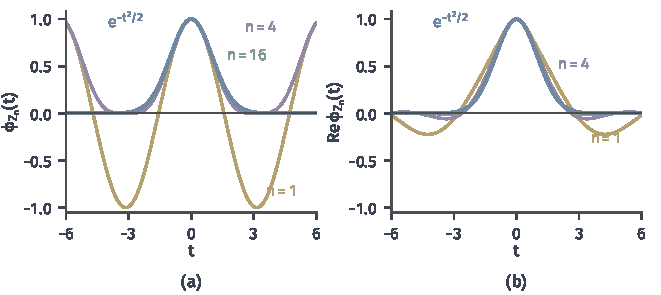
\includegraphics[width=112mm]{figures/07-probability/03-probability-limits/matplotlib/clt-charfun-convergence/figure.pdf}
 \caption{标准化和的特征函数与$\mathrm{e}^{-t^2/2}$（蓝）的比较，$n=1$（黄）、$4$（紫）、$16$（绿；与蓝线几乎重合）。(a)$\pm1$等可能的硬币，$\phi_{Z_n}(t)=\cos(t/\sqrt{n})^{n}$；(b)$\operatorname{Exp}(1)$等待时间，$\phi_{Z_n}(t)=\mathrm{e}^{-\mathrm{i}t\sqrt{n}}(1-\mathrm{i}t/\sqrt{n})^{-n}$的实部。}
 \label{fig:clt-charfun-convergence}
\end{BookInlineFigure}

\subsection{样本平均的正态近似}
\label{sec:clt-sample-mean}

实际使用时，人们关心的是$\bar{X}_n$落在某个区间的概率。把$Z_n\leq x$改写成$\bar{X}_n\leq\mu+x\sigma/\sqrt{n}$，式~\eqref{eq:clt-iid-cdf}就是
\begin{equation}
 \mathbb{P}\Bigl(\bar{X}_n\leq\mu+\frac{x\sigma}{\sqrt{n}}\Bigr)\to\Phi(x),\qquad x\in\mathbb{R} .
 \label{eq:clt-sample-mean}
\end{equation}
人们常把它简写成$\bar{X}_n\approx\mathcal{N}(\mu,\sigma^2/n)$。这个记号的含义是：在$\mu$附近、以$\sigma/\sqrt{n}$为单位量出的阈值上，$\bar{X}_n$的分布函数接近相应的高斯分布函数。

近似的中心是总体均值$\mu$，尺度是$\sigma/\sqrt{n}$，两者都要对。中心取错一个固定量$c$，以$\sigma/\sqrt{n}$为单位就差了$c\sqrt{n}/\sigma$个单位，$n$越大错得越远；尺度用$\sigma/n$或$\sigma$，就回到了第~\ref{sec:clt-scales}节中$a\neq1/2$的情形。

\paragraph{高斯样本：精确}
若$X_i\sim\mathcal{N}(\mu,\sigma^2)$独立，第~\ref{chap:multivariate-distributions}章的线性组合公式给出，对每个$n$，
\[
 \bar{X}_n\sim\mathcal{N}\Bigl(\mu,\frac{\sigma^2}{n}\Bigr),\qquad Z_n\sim\mathcal{N}(0,1) .
\]
这时式~\eqref{eq:clt-sample-mean}左边恒等于$\Phi(x)$，不需要取极限。对一般的样本，式~\eqref{eq:clt-sample-mean}只是$n\to\infty$时的结论，它本身不告诉我们在$n=20$或$n=100$时误差有多大。

\paragraph{二项计数}
设$S\sim\operatorname{Bin}(20,0.3)$，则$np=6$，$np(1-p)=4.2$。精确地，
\[
 \mathbb{P}(S\leq8)\approx0.8867 .
\]
直接套用$\mathcal{N}(6,4.2)$，
\[
 \Phi\Bigl(\frac{8-6}{\sqrt{4.2}}\Bigr)=\Phi(0.976)\approx0.8354 ,
\]
差了约$0.05$。

误差的一个来源是$S$只取整数。$\mathbb{P}(S\leq8)$和$\mathbb{P}(S<9)$是同一个数，阈值在$[8,9)$内任意移动，左边都不变，高斯分布函数却在这一段上从$0.835$升到$0.928$。取中点$8.5$作为阈值，
\[
 \Phi\Bigl(\frac{8.5-6}{\sqrt{4.2}}\Bigr)=\Phi(1.220)\approx0.8887 ,
\]
误差降到$0.002$。这种做法称为\term{连续性修正}（continuity correction）。章首的硬币也一样：$\mathbb{P}(S_{100}\leq55)\approx0.8644$，不修正的近似值是$\Phi(1)\approx0.8413$，修正后是$\Phi(1.1)\approx0.8643$。

图~\ref{fig:clt-binomial-cdf}画出$\operatorname{Bin}(20,0.3)$的分布函数阶梯和两条高斯曲线。不修正的蓝线大致在每级台阶的中点处达到台阶的高度，在整数阈值处偏低；修正后的黄线整体左移半格，在台阶的左端点，也就是整数阈值处，与阶梯的高度相合。连续性修正只是格点分布上的一个经验做法，它不改变极限，也不提供误差保证；有保证的误差界在第~\ref{sec:clt-error}节给出。

\begin{BookInlineFigure}
 \centering
 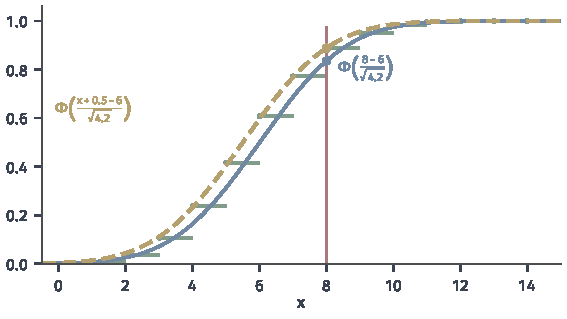
\includegraphics[width=96mm]{figures/07-probability/03-probability-limits/matplotlib/clt-binomial-cdf/figure.pdf}
 \caption{$S\sim\operatorname{Bin}(20,0.3)$的分布函数（绿色阶梯）、高斯近似$\Phi((x-6)/\sqrt{4.2})$（蓝）与连续性修正后的$\Phi((x+0.5-6)/\sqrt{4.2})$（黄色虚线）。红线标出阈值$8$，三点依次为精确值$0.8867$、修正值$0.8887$与未修正值$0.8354$。}
 \label{fig:clt-binomial-cdf}
\end{BookInlineFigure}

\paragraph{需要掷多少次}
正态近似也可以反过来用：给定精度，估计所需的样本量。要使硬币的正面比例与$1/2$相差不超过$0.01$的概率约为$0.95$，由式~\eqref{eq:clt-sample-mean}，需要$0.01$约等于$1.96$个$\sigma/\sqrt{n}$，其中$1.96$是标准高斯分布的$97.5\%$分位数。代入$\sigma=1/2$，
\[
 1.96\cdot\frac{1/2}{\sqrt{n}}=0.01,\qquad n=\Bigl(\frac{1.96\times0.5}{0.01}\Bigr)^2=9604 .
\]

用第~\ref{chap:tail-probabilities}章的Chebyshev不等式也能回答这个问题，而且答案有保证：要使比例偏离$1/2$至少$0.01$的概率不超过$0.05$，只需
\[
 \frac{\sigma^2}{n\cdot0.01^2}=\frac{0.25}{0.0001\,n}\leq0.05,\qquad n\geq50000 .
\]
两个答案相差五倍多。Chebyshev不等式对一切方差为$1/4$的分布都成立，所以保守；正态近似利用了“和接近高斯”这一额外信息，所以省得多，但它只是近似。$n=9604$时这个近似有多准，要等第~\ref{sec:clt-error}节的误差界来回答。

\paragraph{偏斜样本}
指数等待时间没有格点问题，误差来自偏斜。$n=10$时，平均等待时间不超过均值$1$的概率是
\[
 \mathbb{P}(\bar{X}_{10}\leq1)=\mathbb{P}(S_{10}\leq10)\approx0.5421 ,
\]
而式~\eqref{eq:clt-sample-mean}给出$\Phi(0)=0.5$。右偏的分布把中位数拉到均值左边，均值处的分布函数值因此超过$1/2$。图~\ref{fig:clt-gamma-densities}中$n=16$的密度峰仍略偏左，是同一现象。


\section{独立非同分布情形}
\label{sec:clt-non-identical}

一批测量由精度不同的仪器完成，各次误差独立，方差却各不相同；或者每一项的分布本身随总项数变化，像第~\ref{sec:clt-standardization}节的特制硬币。这时没有共同的$\sigma$，标准化只能用总和的标准差。问题变成：各项方差不同，甚至分布随规模改变，什么时候和仍然近似高斯？上一节的特制硬币说明答案不会是“总是”，需要一个条件把“少数几项决定总和”的情形排除掉。

\subsection{三角阵与总方差}
\label{sec:clt-triangular}

各项的分布可以随规模$n$改变，所以把每个规模下的求和项单独列成一行。

\begin{definition}[三角阵]
\label{def:clt-triangular-array}
对每个$n\geq1$，设$k_n$是正整数，$X_{n,1},\dots,X_{n,k_n}$是一组相互独立的随机变量，满足
\begin{equation}
 \mathbb{E}[X_{n,k}]=0,\qquad \sigma_{n,k}^2=\operatorname{Var}(X_{n,k})<\infty .
 \label{eq:clt-array-moments}
\end{equation}
记第$n$行的和与总方差为
\begin{equation}
 S_n=\sum_{k=1}^{k_n}X_{n,k},\qquad s_n^2=\sum_{k=1}^{k_n}\sigma_{n,k}^2 ,
 \label{eq:clt-row-variance}
\end{equation}
并要求$0<s_n^2<\infty$。这样的一族随机变量称为\term{三角阵}（triangular array）。
\end{definition}

名字来自$k_n=n$时的排列方式：第$n$行有$n$项，各行左对齐排成三角形，见图~\ref{fig:clt-triangular-array}。定义只要求同一行内的变量相互独立，不要求不同行之间独立，甚至不要求它们定义在同一个概率空间上。原因是我们只关心每一行的和$S_n$的分布，而$S_n$的分布只由第$n$行的联合分布决定。

\begin{BookInlineFigure}
 \centering
 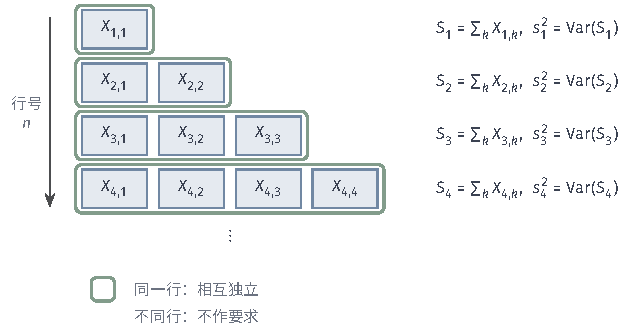
\includegraphics[width=107mm]{figures/07-probability/03-probability-limits/tikz/clt-triangular-array/figure.pdf}
 \caption{三角阵的结构（图中取$k_n=n$）。每一行是一组中心化的求和项，绿框表示行内相互独立；行和$S_n$与总方差$s_n^2$逐行计算，不同行之间不作任何要求。}
 \label{fig:clt-triangular-array}
\end{BookInlineFigure}

由行内独立，$\operatorname{Var}(S_n)=s_n^2$。把各项除以$s_n$，
\[
 \sum_{k=1}^{k_n}\operatorname{Var}\Bigl(\frac{X_{n,k}}{s_n}\Bigr)=\frac{1}{s_n^2}\sum_{k=1}^{k_n}\sigma_{n,k}^2=1 ,
\]
归一化后的各项方差之和为一，$S_n/s_n$均值为零、方差为一。比值$\sigma_{n,k}^2/s_n^2$就是第$k$项在总方差中所占的份额。

\paragraph{独立同分布是特例}
定理~\ref{thm:clt-iid}的情形可以写成三角阵：取$k_n=n$，$X_{n,k}=X_k-\mu$，与$n$无关，则$s_n^2=n\sigma^2$，$S_n/s_n=Z_n$。每一行只是上一行再加一项。三角阵的一般性在于允许各项随$n$整体改变。

\paragraph{三个例子}
本节用下面三个三角阵检验各个条件，它们都满足定义~\ref{def:clt-triangular-array}。
\begin{itemize}
 \item 例A：$X_{n,k}\sim\operatorname{Unif}(-k,k)$，$k=1,\dots,n$。各项有界，方差为$k^2/3$，越往后越大。由$\sum_{k=1}^{n}k^2=n(n+1)(2n+1)/6$，
 \[
  s_n^2=\frac{n(n+1)(2n+1)}{18} .
 \]
 \item 例B：$X_{n,k}\sim\mathcal{N}(0,2^{k})$，$k=1,\dots,n$。方差逐项加倍，$s_n^2=2^{n+1}-2$，最后一项约占总方差的一半。
 \item 例C：$X_{n,k}=B_{n,k}-1/n$，$B_{n,k}\sim\operatorname{Bern}(1/n)$，$k=1,\dots,n$。这是特制硬币的中心化，各项方差都是$\frac1n(1-\frac1n)$，$s_n^2=1-1/n$。
\end{itemize}
例C的行和是$S_n=\operatorname{Bin}(n,1/n)-1$，第~\ref{sec:clt-standardization}节已经看到它的极限不是高斯分布。例B的各项是独立高斯变量，由第~\ref{chap:multivariate-distributions}章，它们的和仍是高斯变量，$S_n\sim\mathcal{N}(0,s_n^2)$，于是对每个$n$都有$S_n/s_n\sim\mathcal{N}(0,1)$。

\subsection{Lindeberg条件}
\label{sec:clt-lindeberg}

例C的毛病在于：总和的波动几乎全部来自“偶尔取到大值”的项。每一项$X_{n,k}$以概率$1/n$取值$1-1/n$，这个值与行的标准差$s_n\approx1$同阶。把方差按取值的大小拆开，例C的方差几乎全部来自那些与$s_n$同阶的取值。要排除这种情形，就要求方差中来自“大值”的部分可以忽略。

\paragraph{截断二阶矩}
固定$\varepsilon>0$，把“大值”理解为绝对值超过$\varepsilon s_n$的取值。每一项的方差拆成两部分，
\[
 \sigma_{n,k}^2=\mathbb{E}\bigl[X_{n,k}^2\mathbf{1}_{\{\lvert X_{n,k}\rvert\leq\varepsilon s_n\}}\bigr]+\mathbb{E}\bigl[X_{n,k}^2\mathbf{1}_{\{\lvert X_{n,k}\rvert>\varepsilon s_n\}}\bigr] .
\]
后一部分是大值贡献的方差。把整行的这部分加起来，再除以总方差，得到大值贡献的份额
\begin{equation}
 L_n(\varepsilon)=\frac{1}{s_n^2}\sum_{k=1}^{k_n}\mathbb{E}\bigl[X_{n,k}^2\mathbf{1}_{\{\lvert X_{n,k}\rvert>\varepsilon s_n\}}\bigr] .
 \label{eq:clt-lindeberg-ratio}
\end{equation}
$L_n(\varepsilon)$在$0$和$1$之间，随$\varepsilon$增大而不增。

\begin{definition}[Lindeberg条件]
\label{def:clt-lindeberg}
称三角阵满足\term{Lindeberg条件}（Lindeberg condition），如果对每个$\varepsilon>0$，
\begin{equation}
 L_n(\varepsilon)\to0\qquad(n\to\infty) .
 \label{eq:clt-lindeberg}
\end{equation}
\end{definition}

条件要求对每个$\varepsilon$都成立，$\varepsilon$越小，被算作大值的范围越宽，要求越严。它说的是：无论把门槛定在总标准差的多小一个比例上，越过门槛的取值所贡献的方差都终将可以忽略。

\paragraph{它推出单项份额趋零}
Lindeberg条件首先保证没有哪一项的方差占总方差的可观份额。对每一项，把方差按$\lvert X_{n,k}\rvert\leq\varepsilon s_n$与否拆开：前一部分不超过$\varepsilon^2s_n^2$，后一部分不超过整行大值贡献之和$s_n^2L_n(\varepsilon)$。于是
\begin{equation}
 \max_{1\leq k\leq k_n}\frac{\sigma_{n,k}^2}{s_n^2}\leq\varepsilon^2+L_n(\varepsilon) .
 \label{eq:clt-max-share}
\end{equation}
令$n\to\infty$，右边的上极限不超过$\varepsilon^2$；$\varepsilon$任意，所以最大份额趋于零。反过来不成立：例C的每一项份额都是$1/n$，趋于零，Lindeberg条件却不成立。单项方差小，不等于大值的贡献小。

\begin{theorem}[Lindeberg中心极限定理]
\label{thm:clt-lindeberg}
设三角阵满足Lindeberg条件~\eqref{eq:clt-lindeberg}。则
\begin{equation}
 \frac{S_n}{s_n}\xrightarrow{\mathrm{d}}\mathcal{N}(0,1) .
 \label{eq:clt-lindeberg-limit}
\end{equation}
\end{theorem}

证明的结构与定理~\ref{thm:clt-iid}相同，仍是比较特征函数的乘积。不同之处在于各因子不再相同，余项要逐项估计后再求和；Lindeberg条件正好控制余项之和。

\begin{proof}
把$X_{n,k}$换成$X_{n,k}/s_n$，可以设$s_n=1$，这时式~\eqref{eq:clt-lindeberg-ratio}中的门槛就是$\varepsilon$。固定$t$和$\varepsilon\in(0,1)$，记$\phi_{n,k}$为$X_{n,k}$的特征函数，并令
\[
 w_{n,k}=1-\frac{t^2\sigma_{n,k}^2}{2} .
\]

第一步，单项误差。在式~\eqref{eq:clt-exp-remainder}中令$x=tX_{n,k}$取期望，与定理~\ref{thm:clt-iid}证明的第一步相同，得到
\[
 \lvert\phi_{n,k}(t)-w_{n,k}\rvert\leq\mathbb{E}\Bigl[\min\Bigl\{\frac{\lvert t\rvert^{3}\lvert X_{n,k}\rvert^{3}}{6},\ t^2X_{n,k}^2\Bigr\}\Bigr] .
\]
在$\{\lvert X_{n,k}\rvert\leq\varepsilon\}$上用三次界，并利用$\lvert X_{n,k}\rvert^3\leq\varepsilon X_{n,k}^2$；在其余部分用二次界。于是
\[
 \lvert\phi_{n,k}(t)-w_{n,k}\rvert\leq\frac{\lvert t\rvert^{3}\varepsilon}{6}\sigma_{n,k}^2+t^2\,\mathbb{E}\bigl[X_{n,k}^2\mathbf{1}_{\{\lvert X_{n,k}\rvert>\varepsilon\}}\bigr] .
\]

第二步，求和。对$k$求和，由$\sum_k\sigma_{n,k}^2=1$与式~\eqref{eq:clt-lindeberg-ratio}，
\[
 \sum_{k=1}^{k_n}\lvert\phi_{n,k}(t)-w_{n,k}\rvert\leq\frac{\lvert t\rvert^{3}\varepsilon}{6}+t^2L_n(\varepsilon) .
\]

第三步，比较乘积。由式~\eqref{eq:clt-max-share}，最大份额趋于零，所以$n$充分大时每个$t^2\sigma_{n,k}^2\leq2$，从而$\lvert w_{n,k}\rvert\leq1$。由行内独立，$\phi_{S_n}(t)=\prod_k\phi_{n,k}(t)$。用引理~\ref{lem:clt-product-difference}，
\[
 \Bigl\lvert\phi_{S_n}(t)-\prod_{k=1}^{k_n}w_{n,k}\Bigr\rvert\leq\frac{\lvert t\rvert^{3}\varepsilon}{6}+t^2L_n(\varepsilon) .
\]
令$n\to\infty$，右边趋于$\lvert t\rvert^3\varepsilon/6$。$\varepsilon$可以任意小，所以左边趋于零。

第四步，乘积的极限。记$a_k=t^2\sigma_{n,k}^2/2\geq0$，则$\sum_ka_k=t^2/2$，而
\[
 \mathrm{e}^{-t^2/2}=\prod_{k=1}^{k_n}\mathrm{e}^{-a_k} .
\]
对$a\geq0$，由带余项的Taylor公式，$\mathrm{e}^{-a}=1-a+\mathrm{e}^{-\xi}a^2/2$，其中$\xi\in(0,a)$，所以$\lvert\mathrm{e}^{-a}-(1-a)\rvert\leq a^2/2$。$\mathrm{e}^{-a_k}$与$w_{n,k}=1-a_k$的模都不超过$1$，再用引理~\ref{lem:clt-product-difference}，
\[
 \Bigl\lvert\prod_{k}w_{n,k}-\mathrm{e}^{-t^2/2}\Bigr\rvert\leq\sum_k\frac{a_k^2}{2}\leq\frac{\max_ka_k}{2}\sum_ka_k=\frac{t^4}{8}\max_k\sigma_{n,k}^2 .
\]
最大份额趋于零，右边趋于零。

第三、四步合起来，$\phi_{S_n}(t)\to\mathrm{e}^{-t^2/2}$对每个$t$成立，由连续性定理得到式~\eqref{eq:clt-lindeberg-limit}。
\end{proof}

证明中Lindeberg条件出现在第三步：小值部分用三次界，贡献至多$\varepsilon$；大值部分只能用二次界，贡献正是$L_n(\varepsilon)$。第四步还需要每项份额都小，这由式~\eqref{eq:clt-max-share}从Lindeberg条件推出。

\paragraph{独立同分布的情形}
对定理~\ref{thm:clt-iid}的三角阵，$Y=(X_1-\mu)/\sigma$，各项同分布，
\[
 L_n(\varepsilon)=\frac{1}{n\sigma^2}\cdot n\,\mathbb{E}\bigl[(X_1-\mu)^2\mathbf{1}_{\{\lvert X_1-\mu\rvert>\varepsilon\sigma\sqrt{n}\}}\bigr]
 =\mathbb{E}\bigl[Y^2\mathbf{1}_{\{\lvert Y\rvert>\varepsilon\sqrt{n}\}}\bigr] .
\]
被积函数被$Y^2$控制，并对每个样本点最终为零，由支配收敛定理，$L_n(\varepsilon)\to0$。所以定理~\ref{thm:clt-iid}是定理~\ref{thm:clt-lindeberg}的特例，二阶矩有限恰好就是独立同分布时的Lindeberg条件。

\paragraph{三个例子的核验}
图~\ref{fig:clt-lindeberg-shares}取$n=20$，$\varepsilon=0.5$，把每一项的方差份额$\sigma_{n,k}^2/s_n^2$画成柱，柱中红色部分是大值的贡献，红色部分之和就是$L_{20}(0.5)$。三个例子的结果分别是
\[
 \text{A}:\ 0.208,\qquad \text{B}:\ 0.749,\qquad \text{C}:\ 0.95 .
\]

\begin{BookInlineFigure}
 \centering
 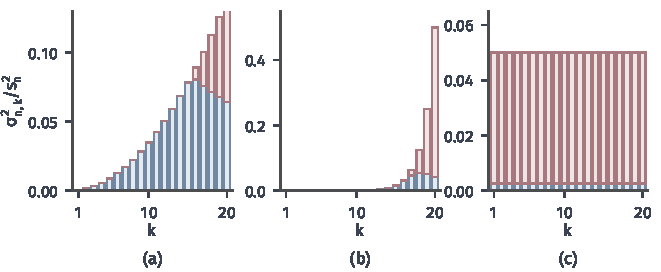
\includegraphics[width=112mm]{figures/07-probability/03-probability-limits/matplotlib/clt-lindeberg-shares/figure.pdf}
 \caption{$n=20$、$\varepsilon=0.5$时各项的方差份额$\sigma_{n,k}^2/s_n^2$。蓝色部分来自$\lvert X_{n,k}\rvert\leq\varepsilon s_n$的取值，红色部分来自$\lvert X_{n,k}\rvert>\varepsilon s_n$的取值，红色之和为$L_{20}(0.5)$。(a)例A，$\operatorname{Unif}(-k,k)$；(b)例B，$\mathcal{N}(0,2^{k})$；(c)例C，中心化的$\operatorname{Bern}(1/20)$。纵轴刻度各不相同。}
 \label{fig:clt-lindeberg-shares}
\end{BookInlineFigure}

例A中$s_{20}^2\approx956.7$，门槛$\varepsilon s_{20}\approx15.5$，只有$k\geq16$的几项可能越过门槛。$\operatorname{Unif}(-k,k)$越过$c<k$的部分贡献
\[
 \mathbb{E}\bigl[X^2\mathbf{1}_{\{\lvert X\rvert>c\}}\bigr]=2\int_c^k\frac{x^2}{2k}\,\mathrm{d}x=\frac{k^3-c^3}{3k} .
\]
代入$c=\varepsilon s_{20}\approx15.465$，$k=16,\dots,20$五项越过门槛的贡献依次约为
\[
 8.28,\quad 23.81,\quad 39.51,\quad 55.44,\quad 71.69 ,
\]
合计约$198.7$，除以$s_{20}^2\approx956.7$得$L_{20}(0.5)\approx0.208$。越往后的项方差越大，越过门槛的部分也越多，图中红色集中在右端。

随着$n$增大，门槛$\varepsilon s_n$按$n^{3/2}$增长，而各项的取值不超过$n$。对$\varepsilon=0.5$，从$n=35$起$\varepsilon s_n\geq n$，没有任何一项能越过门槛，$L_n(0.5)=0$。对任意固定的$\varepsilon>0$同样如此，所以例A满足Lindeberg条件，$S_n/s_n\xrightarrow{\mathrm{d}}\mathcal{N}(0,1)$。

例C中门槛$0.5s_n$小于$0.5$。$n\geq3$时，每一项以概率$1/n$取到的值$1-1/n$越过门槛，另一个取值$-1/n$不越过。所以
\[
 L_n(0.5)=\frac{1}{s_n^2}\cdot n\cdot\frac1n\Bigl(1-\frac1n\Bigr)^{2}=1-\frac1n\to1 .
\]
条件不成立，极限也确实不是高斯分布。

\paragraph{不是必要条件}
例B的$L_n(0.5)$稳定在$0.749$附近，Lindeberg条件不成立，可是$S_n/s_n$对每个$n$都恰好服从$\mathcal{N}(0,1)$。原因是例B的大项本身就是高斯的：最后一项独占一半方差，它的形状直接留在和里，而它碰巧是钟形。所以Lindeberg条件是充分条件，不是中心极限定理的必要条件。

图~\ref{fig:clt-lindeberg-ratio}画出三个例子的$L_n(0.5)$与最大份额随$n$的变化。例A两条曲线都趋于零；例B两条都不趋于零；例C的最大份额$1/n$趋于零，$L_n$却趋于一。

\begin{BookInlineFigure}
 \centering
 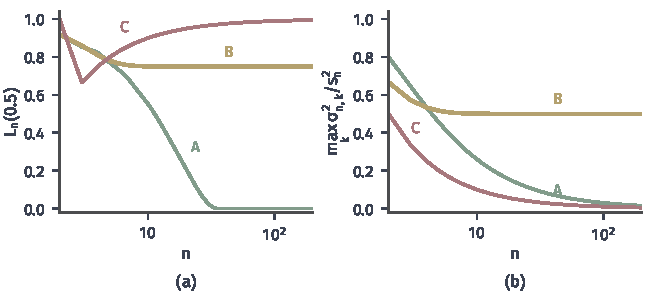
\includegraphics[width=112mm]{figures/07-probability/03-probability-limits/matplotlib/clt-lindeberg-ratio/figure.pdf}
 \caption{三个三角阵的(a)Lindeberg比值$L_n(0.5)$与(b)最大方差份额$\max_k\sigma_{n,k}^2/s_n^2$，$n=2,\dots,200$，横轴为对数刻度。绿为例A，黄为例B，红为例C。}
 \label{fig:clt-lindeberg-ratio}
\end{BookInlineFigure}

例B也说明了缺什么才能反推。若最大份额趋于零，并且$S_n/s_n\xrightarrow{\mathrm{d}}\mathcal{N}(0,1)$，则Lindeberg条件一定成立，这是Feller的逆定理，证明需要更细的特征函数估计，篇幅较长，读者可查阅~\scite{math-kallenberg2021probability}。在“没有一项占优”的前提下，Lindeberg条件就是高斯极限的充要条件；例B不满足这个前提，所以不构成矛盾。

\subsection{Lyapunov条件}
\label{sec:clt-lyapunov}

核验Lindeberg条件要计算截断二阶矩，像例A那样对每一项求越过门槛的部分，往往并不方便。如果各项有略高于二阶的矩，可以用一个更容易计算的量代替它。

\paragraph{用高阶矩压住截断}
在$\{\lvert x\rvert>\varepsilon s_n\}$上，$\lvert x\rvert/(\varepsilon s_n)>1$，于是对任意$\delta>0$，
\[
 x^2\leq x^2\Bigl(\frac{\lvert x\rvert}{\varepsilon s_n}\Bigr)^{\delta}=\frac{\lvert x\rvert^{2+\delta}}{\varepsilon^{\delta}s_n^{\delta}} .
\]
截断二阶矩因此不超过$2+\delta$阶绝对矩除以$\varepsilon^{\delta}s_n^{\delta}$。门槛越高，越过它的取值越大，高阶矩对它们的加权越重，这个不等式正是利用了这一点。

\begin{theorem}[Lyapunov中心极限定理]
\label{thm:clt-lyapunov}
设三角阵的各项具有有限的$2+\delta$阶绝对矩，其中$\delta>0$固定，并且
\begin{equation}
 \Lambda_n(\delta)=\frac{1}{s_n^{2+\delta}}\sum_{k=1}^{k_n}\mathbb{E}\bigl[\lvert X_{n,k}\rvert^{2+\delta}\bigr]\to0 .
 \label{eq:clt-lyapunov}
\end{equation}
则Lindeberg条件成立，从而$S_n/s_n\xrightarrow{\mathrm{d}}\mathcal{N}(0,1)$。
\end{theorem}

条件~\eqref{eq:clt-lyapunov}称为\term{Lyapunov条件}（Lyapunov condition）。

\begin{proof}
对每一项用上面的不等式再取期望，并对$k$求和，
\[
 L_n(\varepsilon)\leq\frac{1}{s_n^2}\sum_{k=1}^{k_n}\frac{\mathbb{E}\bigl[\lvert X_{n,k}\rvert^{2+\delta}\bigr]}{\varepsilon^{\delta}s_n^{\delta}}=\frac{\Lambda_n(\delta)}{\varepsilon^{\delta}} .
\]
对每个固定的$\varepsilon>0$，右边趋于零，这就是Lindeberg条件。再由定理~\ref{thm:clt-lindeberg}得到结论。
\end{proof}

\paragraph{例A的三阶矩}
取$\delta=1$。$\operatorname{Unif}(-k,k)$的三阶绝对矩是
\[
 \mathbb{E}\bigl[\lvert X\rvert^{3}\bigr]=\frac{1}{2k}\int_{-k}^{k}\lvert x\rvert^{3}\,\mathrm{d}x=\frac{k^3}{4} .
\]
由$\sum_{k=1}^{n}k^3=\bigl(n(n+1)/2\bigr)^2$与$s_n^2=n(n+1)(2n+1)/18$，
\[
 \Lambda_n(1)=\frac{n^2(n+1)^2/16}{\bigl(n(n+1)(2n+1)/18\bigr)^{3/2}}\approx\frac{27}{16\sqrt{n}} .
\]
$n=20,100,1000$时，精确值分别约为$0.373$、$0.168$、$0.053$，按$1/\sqrt{n}$趋于零。这里不需要像核验Lindeberg条件那样找出哪些项越过门槛，只要把各项的矩加起来。

\paragraph{有界项}
若存在常数$M$使$\lvert X_{n,k}\rvert\leq M$，并且$s_n\to\infty$，则$\lvert X_{n,k}\rvert^3\leq MX_{n,k}^2$，取期望得
\[
 \mathbb{E}\bigl[\lvert X_{n,k}\rvert^{3}\bigr]\leq M\sigma_{n,k}^2 .
\]
对$k$求和再除以$s_n^3$，
\[
 \Lambda_n(1)\leq\frac{M s_n^2}{s_n^3}=\frac{M}{s_n}\to0 .
\]
所以总方差趋于无穷的一致有界独立项，标准化和总趋于标准高斯分布。例C的各项也有界，但$s_n^2=1-1/n$不趋于无穷，这个推理不适用。

\paragraph{两个条件的比较}
Lyapunov条件多要求了$2+\delta$阶矩，换来的是只需计算未截断的矩之和。它比Lindeberg条件严格地强：设$X_1,X_2,\dots$独立同分布，方差有限，但对每个$\delta>0$都有$\mathbb{E}[\lvert X_1\rvert^{2+\delta}]=\infty$，例如密度在$\lvert x\rvert>\mathrm{e}$上与$1/(\lvert x\rvert^3\ln^2\lvert x\rvert)$成正比的对称分布。这时Lyapunov条件无从谈起，而独立同分布时Lindeberg条件总成立，中心极限定理照样成立。图~\ref{fig:clt-condition-map}汇总了本节的几个条件与结论之间的推出关系。

\begin{BookInlineFigure}
 \centering
 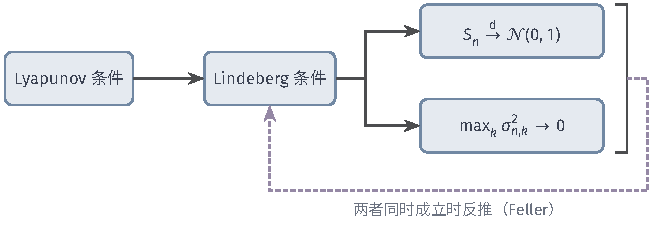
\includegraphics[width=111mm]{figures/07-probability/03-probability-limits/tikz/clt-condition-map/figure.pdf}
 \caption{三角阵各条件与结论的关系（行内独立、中心化、$s_n=1$）。实线箭头表示推出；紫色虚线表示Feller逆定理：高斯极限与最大份额趋零同时成立时，可以反推Lindeberg条件。单有高斯极限推不出Lindeberg条件，例B即是。}
 \label{fig:clt-condition-map}
\end{BookInlineFigure}

这些条件都只是充分条件，或者在附加前提下才是充要条件。把它们当作中心极限定理的必要条件，就会像例B那样误判；反过来，看到“每项方差都很小”就断言高斯极限，又会在例C上出错。


\section{多元中心极限定理}
\label{sec:clt-multivariate}

掷$n$次骰子，记下六个面各出现了多少次；或者同时测量一批零件的长度和重量。这时每次观测是一个向量，平均也是向量。各分量的平均分别近似高斯还不够，我们还想知道它们的偏差怎样联合分布：长度偏大时重量是否也偏大，六个频率之和恒为一这一约束又怎样体现在极限里。

设$\bm{X}_1,\bm{X}_2,\dots$是$\mathbb{R}^{d}$中独立同分布的随机向量，维数$d$固定，$\mathbb{E}[\lVert\bm{X}_1\rVert_2^2]<\infty$。记均值向量为$\bm{\mu}$，协方差矩阵为$\bm{\Sigma}$（粗体大写表示$d\times d$矩阵），样本平均为
\[
 \bar{\bm{X}}_n=\frac1n\sum_{i=1}^{n}\bm{X}_i .
\]
要研究的对象是$\sqrt{n}(\bar{\bm{X}}_n-\bm{\mu})$。这里不除以标准差：向量没有单一的标准差，$\bm{\Sigma}$还可能不可逆。极限中会直接出现$\bm{\Sigma}$本身。

\paragraph{两枚硬币的例子}
设$\xi,\eta$独立，各以$1/2$的概率取$\pm1$，令$\bm{X}=(\xi,\ \xi+\eta)^{\top}$。两个分量共享$\xi$，所以正相关。直接计算，$\bm{\mu}=\bm{0}$，
\[
 \operatorname{Var}(\xi)=1,\qquad \operatorname{Var}(\xi+\eta)=2,\qquad \operatorname{Cov}(\xi,\xi+\eta)=\operatorname{Var}(\xi)=1 ,
\]
即
\[
 \bm{\Sigma}=\begin{bmatrix}1&1\\1&2\end{bmatrix} .
\]
本节还用一个退化的对照：$\bm{X}=(\xi,\ 2\xi)^{\top}$，协方差矩阵的各元为$1,2,2,4$，行列式为零。

\subsection{方向投影}
\label{sec:clt-projection}

向量的分布不容易直接处理，可以先把它投到各个方向上，变成标量问题。固定$\bm{a}\in\mathbb{R}^{d}$，投影$\bm{a}^{\top}\bm{X}_i$是独立同分布的实随机变量。由第~\ref{chap:random-vectors}章的均值与协方差的线性规则，
\[
 \mathbb{E}[\bm{a}^{\top}\bm{X}_i]=\bm{a}^{\top}\bm{\mu},\qquad \operatorname{Var}(\bm{a}^{\top}\bm{X}_i)=\bm{a}^{\top}\bm{\Sigma}\bm{a} .
\]
投影与平均可以交换，$\bm{a}^{\top}\sqrt{n}(\bar{\bm{X}}_n-\bm{\mu})$正是投影序列的$\sqrt{n}$倍平均偏差。按$\bm{a}^{\top}\bm{\Sigma}\bm{a}$是否为零分两种情形。

\paragraph{正方差方向}
若$\bm{a}^{\top}\bm{\Sigma}\bm{a}>0$，投影序列满足定理~\ref{thm:clt-iid}的全部条件，所以
\[
 \frac{\sqrt{n}\,\bm{a}^{\top}(\bar{\bm{X}}_n-\bm{\mu})}{\sqrt{\bm{a}^{\top}\bm{\Sigma}\bm{a}}}\xrightarrow{\mathrm{d}}\mathcal{N}(0,1) .
\]
记左边为$W_n$，再乘回常数$c=\sqrt{\bm{a}^{\top}\bm{\Sigma}\bm{a}}>0$。对每个$x$，
\[
 \mathbb{P}(cW_n\leq x)=\mathbb{P}\Bigl(W_n\leq\frac{x}{c}\Bigr)\to\Phi\Bigl(\frac{x}{c}\Bigr) ,
\]
右边是$\mathcal{N}(0,c^2)$的分布函数。于是
\begin{equation}
 \sqrt{n}\,\bm{a}^{\top}(\bar{\bm{X}}_n-\bm{\mu})\xrightarrow{\mathrm{d}}\mathcal{N}(0,\bm{a}^{\top}\bm{\Sigma}\bm{a}) .
 \label{eq:clt-projection}
\end{equation}

\paragraph{零方差方向}
若$\bm{a}^{\top}\bm{\Sigma}\bm{a}=0$，标准化要除以零，不能套用。这时$\bm{a}^{\top}(\bm{X}_i-\bm{\mu})$均值为零、方差为零，几乎必然等于零。于是对每个$n$，
\[
 \sqrt{n}\,\bm{a}^{\top}(\bar{\bm{X}}_n-\bm{\mu})=\frac{1}{\sqrt{n}}\sum_{i=1}^{n}\bm{a}^{\top}(\bm{X}_i-\bm{\mu})=0\quad\text{几乎必然} .
\]
它的分布恒为$0$处的单点分布，当然依分布收敛到这个单点分布。按第~\ref{sec:clt-standardization}节的约定，单点分布就是$\mathcal{N}(0,0)$，所以式~\eqref{eq:clt-projection}在零方差方向也成立。

\paragraph{两枚硬币的投影}
对$\bm{X}=(\xi,\ \xi+\eta)^{\top}$，三个方向上的极限方差分别是
\[
 \bm{a}=(1,0)^{\top}:\ 1,\qquad \bm{a}=(0,1)^{\top}:\ 2,\qquad \bm{a}=\tfrac{1}{\sqrt2}(1,-1)^{\top}:\ \tfrac12(1-2+2)=\tfrac12 .
\]
最后一个方向是两分量之差，$\xi-(\xi+\eta)=-\eta$，方差本来就是$1$，除以$(\sqrt2)^2$后为$1/2$。图~\ref{fig:clt-projections}用$n=100$、$1500$次重复模拟检验这三个结论，三个直方图的样本方差分别为$0.98$、$1.99$、$0.47$。

\begin{BookInlineFigure}
 \centering
 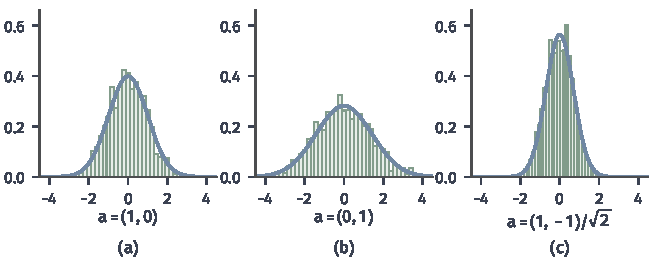
\includegraphics[width=112mm]{figures/07-probability/03-probability-limits/matplotlib/clt-projections/figure.pdf}
 \caption{$\bm{X}=(\xi,\xi+\eta)^{\top}$、$n=100$时$\bm{a}^{\top}\sqrt{n}\,\bar{\bm{X}}_n$的直方图（浅绿，$1500$次重复，种子$3$，每个格点一个柱）与$\mathcal{N}(0,\bm{a}^{\top}\bm{\Sigma}\bm{a})$的密度（蓝）。(a)$\bm{a}=(1,0)^{\top}$，方差$1$；(b)$\bm{a}=(0,1)^{\top}$，方差$2$；(c)$\bm{a}=(1,-1)^{\top}/\sqrt2$，方差$1/2$。}
 \label{fig:clt-projections}
\end{BookInlineFigure}

对退化的$\bm{X}=(\xi,\ 2\xi)^{\top}$，方向$\bm{a}=(2,-1)^{\top}$给出$\bm{a}^{\top}\bm{X}=2\xi-2\xi=0$，这是零方差方向；与它垂直的方向$(1,2)^{\top}/\sqrt5$上，投影是$\sqrt5\,\xi$，方差为$5$。

\subsection{联合高斯极限}
\label{sec:clt-joint}

每个方向上的极限都是高斯的，方差由同一个矩阵$\bm{\Sigma}$按$\bm{a}^{\top}\bm{\Sigma}\bm{a}$给出。第~\ref{chap:multivariate-distributions}章说明，若$\bm{W}\sim\mathcal{N}(\bm{0},\bm{\Sigma})$，则对每个$\bm{a}$，
\begin{equation}
 \bm{a}^{\top}\bm{W}\sim\mathcal{N}(0,\bm{a}^{\top}\bm{\Sigma}\bm{a}) .
 \label{eq:clt-gauss-projection}
\end{equation}
所以各方向的极限恰好是同一个高斯向量$\bm{W}$的各个投影。Cramér--Wold判据说，在固定维数中，所有方向的投影依分布收敛到同一个向量的投影，就足以推出向量本身依分布收敛。

\begin{theorem}[多元中心极限定理]
\label{thm:clt-multivariate}
设$\bm{X}_1,\bm{X}_2,\dots$是$\mathbb{R}^{d}$中独立同分布的随机向量，$\mathbb{E}[\lVert\bm{X}_1\rVert_2^2]<\infty$，均值为$\bm{\mu}$，协方差矩阵为$\bm{\Sigma}$。则
\begin{equation}
 \sqrt{n}\,(\bar{\bm{X}}_n-\bm{\mu})\xrightarrow{\mathrm{d}}\mathcal{N}(\bm{0},\bm{\Sigma}) .
 \label{eq:clt-multivariate}
\end{equation}
\end{theorem}

这个结论称为\term{多元中心极限定理}（multivariate central limit theorem）。

\begin{proof}
设$\bm{W}\sim\mathcal{N}(\bm{0},\bm{\Sigma})$。对每个$\bm{a}\in\mathbb{R}^{d}$，由式~\eqref{eq:clt-projection}，投影$\bm{a}^{\top}\sqrt{n}(\bar{\bm{X}}_n-\bm{\mu})$依分布收敛到$\mathcal{N}(0,\bm{a}^{\top}\bm{\Sigma}\bm{a})$，正方差与零方差方向都包括在内。由式~\eqref{eq:clt-gauss-projection}，这个极限就是$\bm{a}^{\top}\bm{W}$的分布。由Cramér--Wold判据，$\sqrt{n}(\bar{\bm{X}}_n-\bm{\mu})\xrightarrow{\mathrm{d}}\bm{W}$。
\end{proof}

\paragraph{为什么要看所有方向}
只看坐标方向，得到的是每个分量各自的极限，即边缘分布的收敛。第~\ref{chap:weak-convergence-of-distributions}章说明，边缘收敛不能确定分量之间的配对方式。两枚硬币的例子里，两个分量的极限分别是$\mathcal{N}(0,1)$与$\mathcal{N}(0,2)$；它们是相互独立，还是相关系数为$1/\sqrt2$，只有斜方向（例如图~\ref{fig:clt-projections}(c)）的方差能分辨：独立时差的方差应是$\frac12(1+2)=\frac32$，实际是$\frac12$。定理的证明用到了全部方向，所以得到的是联合极限，相关结构由$\bm{\Sigma}$的非对角元保留下来。

图~\ref{fig:clt-bivariate-scatter}(a)把同一批模拟的点$\sqrt{n}\,\bar{\bm{X}}_n$画在平面上，点云沿主对角方向拉长。$\mathcal{N}(\bm{0},\bm{\Sigma})$在马氏距离$1$与$2$以内的概率是$1-\mathrm{e}^{-1/2}\approx0.393$与$1-\mathrm{e}^{-2}\approx0.865$，模拟点落在这两个椭圆内（含边界）的比例是$0.398$与$0.885$，边界上的格点使后者略偏大。点排成格子，因为$n=100$时每个分量只取间距为$0.2$的格点值；依分布收敛并不要求有限$n$的分布有密度。

\begin{BookInlineFigure}
 \centering
 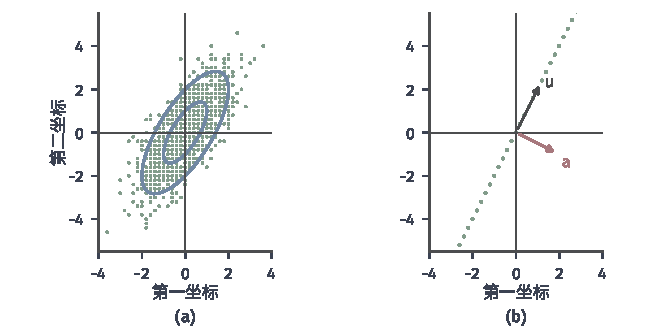
\includegraphics[width=112mm]{figures/07-probability/03-probability-limits/matplotlib/clt-bivariate-scatter/figure.pdf}
 \caption{$n=100$时$\sqrt{n}\,\bar{\bm{X}}_n$的$1500$个模拟点（绿，种子$3$）。(a)$\bm{X}=(\xi,\xi+\eta)^{\top}$，蓝色椭圆是$\mathcal{N}(\bm{0},\bm{\Sigma})$在马氏距离$1$与$2$处的等高线；(b)$\bm{X}=(\xi,2\xi)^{\top}$，点全部落在直线$y=2x$上，红色箭头$\bm{a}$是零方差方向$(2,-1)^{\top}/\sqrt5$，灰色箭头$\bm{u}$是直线方向$(1,2)^{\top}/\sqrt5$。}
 \label{fig:clt-bivariate-scatter}
\end{BookInlineFigure}

\paragraph{奇异的协方差矩阵}
定理不要求$\bm{\Sigma}$可逆。退化例子中$\bm{\Sigma}$的秩为一，极限$\mathcal{N}(\bm{0},\bm{\Sigma})$是第~\ref{chap:multivariate-distributions}章的退化高斯分布，全部质量在直线$\{t(1,2)^{\top}:t\in\mathbb{R}\}$上，在平面上没有密度。图~\ref{fig:clt-bivariate-scatter}(b)中有限$n$的点也都在这条直线上。若要写出标准化的形式$\bm{\Sigma}^{-1/2}\sqrt{n}(\bar{\bm{X}}_n-\bm{\mu})$，就必须假设$\bm{\Sigma}$可逆；式~\eqref{eq:clt-multivariate}的写法避开了这个假设。

\paragraph{骰子的频率}
掷一枚均匀骰子$n$次，令$\bm{X}_i\in\mathbb{R}^{6}$是第$i$次结果的示性向量：出现第$j$面时第$j$个分量为$1$，其余为$0$。$\bar{\bm{X}}_n$就是六个面的频率向量，$n\bar{\bm{X}}_n\sim\operatorname{Mult}(n,\bm{p})$，$\bm{p}=\frac16\bm{1}$。由$X_{i,j}X_{i,k}=0$（$j\neq k$）与$X_{i,j}^2=X_{i,j}$，
\[
 \bm{\Sigma}=\operatorname{diag}(\bm{p})-\bm{p}\bm{p}^{\top},\qquad \Sigma_{j,j}=\frac16-\frac1{36}=\frac{5}{36},\qquad \Sigma_{j,k}=-\frac{1}{36}\ (j\neq k) .
\]
由定理~\ref{thm:clt-multivariate}，$\sqrt{n}(\bar{\bm{X}}_n-\bm{p})\xrightarrow{\mathrm{d}}\mathcal{N}(\bm{0},\bm{\Sigma})$。频率之和恒为一，所以$\bm{1}^{\top}(\bm{X}_i-\bm{p})=0$，$\bm{1}$是零方差方向，$\bm{\Sigma}\bm{1}=\bm{0}$。极限分布集中在“六个偏差之和为零”的五维子空间上，各频率偏差之间是负相关：一个面出现得多，其余的面就只能少。

\paragraph{维数固定}
定理中的$d$在$n\to\infty$时保持不变。它不说明维数随样本量一同增长时会怎样，也不涉及部分和作为$n$的函数、整条随机路径的极限形状；后者需要在函数空间中讨论收敛，超出了有限维概率极限的范围。


\section{正态近似误差}
\label{sec:clt-error}

中心极限定理是$n\to\infty$时的结论，它保证误差趋于零，却不告诉我们$n=100$时误差是$0.04$还是$0.4$。前面的例子已经给出一些具体数字：$\operatorname{Bin}(20,0.3)$在阈值$8$处差了$0.05$，十个指数等待时间的平均在均值处差了$0.042$。本节先确定比较的是哪一种误差，再在多一阶矩的条件下给出对所有阈值同时成立的上界。

\paragraph{比较什么}
设$F_n$是$Z_n$的分布函数。最常用的比较对象是两条分布函数之间的最大竖直距离
\begin{equation}
 D_n=\sup_{x\in\mathbb{R}}\bigl\lvert F_n(x)-\Phi(x)\bigr\rvert .
 \label{eq:clt-kolmogorov}
\end{equation}
它控制所有形如$\{Z_n\leq x\}$的事件，从而控制所有区间事件：$\mathbb{P}(a<Z_n\leq b)$与$\Phi(b)-\Phi(a)$之差不超过$2D_n$。由式~\eqref{eq:clt-iid-cdf}与$\Phi$的连续性，可以证明$D_n\to0$，但定理本身不给出速度。怎样利用这样的近似构造区间并评价其可靠性，属于统计推断的问题，可参考\BookChapterRef{chap:parametric-statistical-inference}{卷八第1章“参数化统计推断”}；这里只研究概率误差本身。

\subsection{Berry--Esseen界}
\label{sec:clt-berry-esseen}

定理~\ref{thm:clt-iid}的证明里，单个因子的误差用了二次界，因为只知道二阶矩。如果三阶绝对矩有限，就可以用三次界：每个因子的误差约为$\lvert t\rvert^3\mathbb{E}[\lvert Y\rvert^3]/(6n^{3/2})$，$n$个因子累计为$\lvert t\rvert^3\mathbb{E}[\lvert Y\rvert^3]/(6\sqrt{n})$。特征函数之差按$1/\sqrt{n}$缩小，分布函数之差也应当如此。

\begin{theorem}[Berry--Esseen界]
\label{thm:clt-berry-esseen}
设$X_1,X_2,\dots$独立同分布，方差$\sigma^2>0$，三阶绝对中心矩$\rho=\mathbb{E}[\lvert X_1-\mu\rvert^{3}]<\infty$。则存在与分布无关的常数$C$，使对每个$n\geq1$，
\begin{equation}
 \sup_{x\in\mathbb{R}}\bigl\lvert\mathbb{P}(Z_n\leq x)-\Phi(x)\bigr\rvert\leq\frac{C\rho}{\sigma^{3}\sqrt{n}} .
 \label{eq:clt-berry-esseen}
\end{equation}
\end{theorem}

这个上界称为\term{Berry--Esseen界}（Berry-Esseen bound）。目前已知可以取$C=0.4748$。证明的关键是一个光滑化不等式：把分布函数之差用特征函数之差在原点附近的积分来控制，再代入上面的三阶估计。这一不等式的推导与常数的优化都较长，读者可查阅~\scite{math-kallenberg2021probability}。

\paragraph{界的含义}
式~\eqref{eq:clt-berry-esseen}有三个特点。它对所有阈值$x$同时成立，所以是一致的；它控制的是概率之差，是绝对误差；它以$1/\sqrt{n}$的速度缩小，样本量变成四倍，误差界减半。分布的影响全部集中在比值$\rho/\sigma^3$上，这是标准化变量$Y$的三阶绝对矩$\mathbb{E}[\lvert Y\rvert^3]$。

这个比值至少是$1$。函数$u\mapsto u^{3/2}$在$[0,\infty)$上是凸函数，对非负变量$Y^2$用Jensen不等式，
\[
 \mathbb{E}\bigl[\lvert Y\rvert^{3}\bigr]=\mathbb{E}\bigl[(Y^2)^{3/2}\bigr]\geq\bigl(\mathbb{E}[Y^2]\bigr)^{3/2}=1 .
\]
等号对以等概率取$\pm1$的$Y$成立。比值越大，说明单项的取值越偏离“正负各一个标准差”，界越松。

\paragraph{三个分布的比值}
对$X\sim\operatorname{Bern}(p)$，$\lvert X-p\rvert$以概率$p$取$1-p$，以概率$1-p$取$p$，记$q=1-p$，
\[
 \rho=pq^3+qp^3=pq(p^2+q^2),\qquad \frac{\rho}{\sigma^3}=\frac{p^2+q^2}{\sqrt{pq}} .
\]
$p=1/2$时比值为$1$，$p=1/10$时为$0.82/0.3\approx2.733$。对$X\sim\operatorname{Exp}(1)$，$\sigma=1$，把积分在$x=1$处分开，
\[
 \int_1^{\infty}(x-1)^3\mathrm{e}^{-x}\,\mathrm{d}x=\frac{6}{\mathrm{e}},\qquad \int_0^1(1-x)^3\mathrm{e}^{-x}\,\mathrm{d}x=\frac{6}{\mathrm{e}}-2 ,
\]
前一个积分换元$u=x-1$后是$\mathrm{e}^{-1}\int_0^\infty u^3\mathrm{e}^{-u}\,\mathrm{d}u$，后一个由三次分部积分得到。合起来$\rho=12/\mathrm{e}-2\approx2.415$。

表~\ref{tab:clt-berry-esseen}比较$n=100$时的上界与精确的最大误差。最大误差由精确分布在所有跳点两侧逐一比较得到；指数情形用$\operatorname{Gamma}(n,1)$的分布函数在细网格上计算。

\begin{BookInlineTable}
 \centering
 \caption{$n=100$时Berry--Esseen上界（$C=0.4748$）与精确最大误差$D_{100}$的比较。}
 \label{tab:clt-berry-esseen}
 \begin{tabular}{lccc}
 \toprule
 单项分布 & $\rho/\sigma^3$ & 上界$C\rho/(\sigma^3\sqrt{100})$ & 精确$D_{100}$ \\
 \midrule
 $\operatorname{Bern}(1/2)$ & $1$ & $0.0475$ & $0.0398$ \\
 $\operatorname{Bern}(1/10)$ & $2.733$ & $0.130$ & $0.0832$ \\
 $\operatorname{Exp}(1)$ & $2.415$ & $0.115$ & $0.0133$ \\
 \bottomrule
 \end{tabular}
\end{BookInlineTable}

回到第~\ref{sec:clt-sample-mean}节掷$9604$次硬币的问题。比值为$1$，每个分布函数值的误差不超过$0.4748/\sqrt{9604}\approx0.0048$，区间概率是两个分布函数值之差，误差不超过$0.0097$。所以那里的“约为$0.95$”可以确切地写成“在$0.94$与$0.96$之间”。

表中硬币的上界只比实际误差大约五分之一，指数等待时间的上界却大了八倍多。图~\ref{fig:clt-berry-esseen-rate}在双对数坐标中画出$n$从$1$到$1000$的情形，所有误差曲线都以斜率$-1/2$下降，与上界平行，各自始终在自己的上界之下。

\begin{BookInlineFigure}
 \centering
 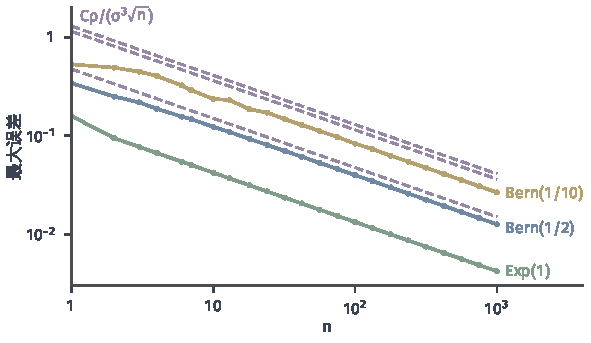
\includegraphics[width=100mm]{figures/07-probability/03-probability-limits/matplotlib/clt-berry-esseen-rate/figure.pdf}
 \caption{标准化和与$\mathcal{N}(0,1)$的精确最大误差$D_n$随$n$的变化，双对数坐标。蓝为$\operatorname{Bern}(1/2)$，黄为$\operatorname{Bern}(1/10)$，绿为$\operatorname{Exp}(1)$。紫色虚线是对应的Berry--Esseen上界$0.4748\rho/(\sigma^3\sqrt{n})$，自上而下依次属于$\operatorname{Bern}(1/10)$、$\operatorname{Exp}(1)$与$\operatorname{Bern}(1/2)$。}
 \label{fig:clt-berry-esseen-rate}
\end{BookInlineFigure}

\paragraph{速度不能更快}
$1/\sqrt{n}$的速度一般不能改进，硬币就是例子。$n$为偶数时，$Z_n$在$0$处有一个原子，质量是$\mathbb{P}(S_n=n/2)$，分布函数在那里跳起这么高，而$\Phi$是连续的。在跳点处，$F_n$的左极限与右值相差这个跳跃，它们与同一个数$\Phi(0)$的距离至少有一个不小于跳跃的一半。所以
\[
 D_n\geq\frac12\,\mathbb{P}\Bigl(S_n=\frac n2\Bigr)=\frac12\binom{n}{n/2}2^{-n} .
\]
$n=100$时右边是$\frac12\times0.0796=0.0398$，正好是表~\ref{tab:clt-berry-esseen}中的精确值。由Stirling公式，$\binom{n}{n/2}2^{-n}\approx\sqrt{2/(\pi n)}$，于是$D_n$至少约为$1/\sqrt{2\pi n}\approx0.399/\sqrt{n}$。这也说明常数$C$不能小于约$0.399$。

\paragraph{误差出现在哪里}
最大误差只是一个数，图~\ref{fig:clt-error-profile}画出带符号的误差$F_n(x)-\Phi(x)$随阈值的变化。指数等待时间的误差是一条光滑的波形，在中心附近为正、两侧为负，这是右偏造成的：均值处的分布函数值$0.542$超过$1/2$。硬币的误差是锯齿形，每过一个格点跳一次，幅度在中心最大；这一误差来自格点结构，任何光滑的近似都无法消除，连续性修正只是把阈值放到台阶中间以减小它。

\begin{BookInlineFigure}
 \centering
 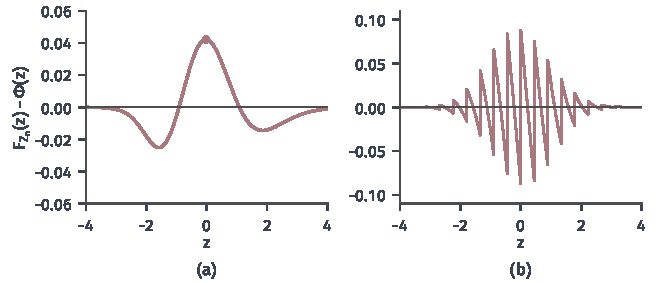
\includegraphics[width=112mm]{figures/07-probability/03-probability-limits/matplotlib/clt-error-profile/figure.pdf}
 \caption{带符号的误差$F_{Z_n}(z)-\Phi(z)$。(a)$\operatorname{Exp}(1)$，$n=10$，红点为最大误差$0.042$，位于$z\approx0$；(b)$\operatorname{Bern}(1/2)$，$n=20$，误差在每个格点处跳跃，最大约$0.088$。}
 \label{fig:clt-error-profile}
\end{BookInlineFigure}

\paragraph{非同分布的情形}
三角阵也有类似的界：若各项三阶绝对矩有限，$S_n/s_n$与$\mathcal{N}(0,1)$的分布函数最大距离不超过一个通用常数乘以
\[
 \frac{1}{s_n^3}\sum_{k=1}^{k_n}\mathbb{E}\bigl[\lvert X_{n,k}\rvert^{3}\bigr] ,
\]
这正是第~\ref{sec:clt-lyapunov}节$\delta=1$时的Lyapunov比值$\Lambda_n(1)$。Lyapunov条件因此不只保证收敛，在$\delta=1$时还直接给出了误差的量级。例A中$\Lambda_n(1)\approx27/(16\sqrt{n})$，误差也按$1/\sqrt{n}$缩小。

\subsection{近似的适用范围}
\label{sec:clt-applicability}

“正态近似可用”这句话要说清楚用于什么精度。表~\ref{tab:clt-accuracy}列出三种不同的要求。前两种已经讨论过；第三种在计算罕见事件的概率时常常遇到，Berry--Esseen界对它几乎没有帮助。

\begin{BookInlineTable}
 \centering
 \caption{正态近似的三种精度要求。}
 \label{tab:clt-accuracy}
 \begin{tabular}{lll}
 \toprule
 精度要求 & 含义 & 本章的依据 \\
 \midrule
 渐近收敛 & 误差随$n$趋于零 & 二阶矩或Lindeberg条件 \\
 一致绝对误差 & 给定$n$时的误差上界 & 三阶矩，Berry--Esseen界 \\
 尾概率相对误差 & 近似值与真值之比 & 本章没有给出 \\
 \bottomrule
 \end{tabular}
\end{BookInlineTable}

\paragraph{小尾概率}
设$p_n(z)=\mathbb{P}(Z_n\geq z)$。由式~\eqref{eq:clt-berry-esseen}，取左极限后同样有
\[
 \bigl\lvert p_n(z)-(1-\Phi(z))\bigr\rvert\leq\frac{C\rho}{\sigma^3\sqrt{n}} ,
\]
右边与$z$无关。当$z$较大时，$1-\Phi(z)$本身可能是$10^{-4}$甚至更小，而右边是$0.1$量级，这个界不能说明近似值有一位有效数字是对的。

十个指数等待时间的精确右尾与高斯近似是
\[
 \begin{aligned}
 z=2:&\quad 0.0369 &&\text{对}\quad 0.0228,\\
 z=3:&\quad 0.00672 &&\text{对}\quad 0.00135,\\
 z=4:&\quad 1.01\times10^{-3} &&\text{对}\quad 3.17\times10^{-5},\\
 z=5:&\quad 1.29\times10^{-4} &&\text{对}\quad 2.87\times10^{-7} .
 \end{aligned}
\]
比值依次约为$1.6$、$5.0$、$32$、$450$。绝对误差都不超过$0.015$，与Berry--Esseen界并不矛盾；相对误差却越来越大。左尾的情形更极端：$S_{10}>0$，所以$Z_{10}>-\sqrt{10}$，$\mathbb{P}(Z_{10}\leq-\sqrt{10})=0$，而高斯近似给出$\Phi(-\sqrt{10})\approx7.8\times10^{-4}$。

图~\ref{fig:clt-relative-tail}在对数纵轴上画出两侧的尾部。右偏的分布右尾比高斯厚，左尾比高斯薄而且在有限处截断。对数坐标暴露出来的这些差别，在普通坐标中都挤在零附近，看不出来。

\begin{BookInlineFigure}
 \centering
 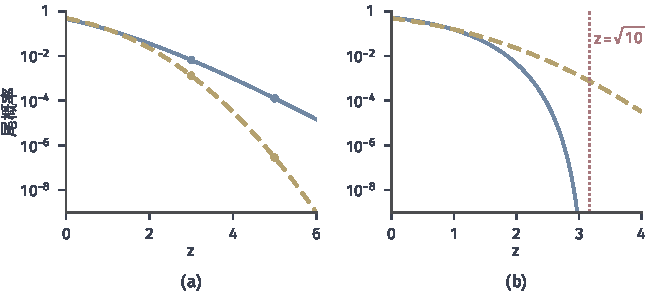
\includegraphics[width=112mm]{figures/07-probability/03-probability-limits/matplotlib/clt-relative-tail/figure.pdf}
 \caption{$n=10$个$\operatorname{Exp}(1)$之和标准化后的尾概率，纵轴为对数刻度。蓝线为精确值，黄色虚线为高斯近似。(a)右尾$\mathbb{P}(Z_{10}\geq z)$与$1-\Phi(z)$，圆点标出$z=3,5$；(b)左尾$\mathbb{P}(Z_{10}\leq-z)$与$\Phi(-z)$，精确左尾在$z=\sqrt{10}$（红色点线）处降为零。}
 \label{fig:clt-relative-tail}
\end{BookInlineFigure}

中心极限定理描述的是距中心几个标准差以内的“典型”波动；离中心越远，概率越依赖单项分布的尾部形状，而不仅是均值和方差。估计罕见事件的概率，应当直接计算精确分布，或使用第~\ref{chap:tail-probabilities}章基于指数矩的上界，它们的误差是按尾概率本身的大小来衡量的。

\paragraph{三阶矩无穷的情形}
Berry--Esseen界需要三阶绝对矩，中心极限定理只需要二阶矩，两者之间有一段空隙。取第~\ref{chap:tail-probabilities}章参数为$3$的Pareto分布，配上等概率的正负号，得到密度
\[
 f(x)=\frac32\lvert x\rvert^{-4},\qquad \lvert x\rvert\geq1 .
\]
它关于原点对称，均值为零。二阶矩与三阶绝对矩分别是
\[
 \mathbb{E}[X^2]=2\int_1^{\infty}x^2\cdot\frac32x^{-4}\,\mathrm{d}x=3,\qquad
 \mathbb{E}\bigl[\lvert X\rvert^3\bigr]=3\int_1^{\infty}x^{-1}\,\mathrm{d}x=\infty .
\]

方差有限，定理~\ref{thm:clt-iid}适用，$S_n/\sqrt{3n}\xrightarrow{\mathrm{d}}\mathcal{N}(0,1)$。图~\ref{fig:clt-pareto-third}的模拟也显示出钟形。可是$\rho=\infty$，式~\eqref{eq:clt-berry-esseen}的右边是无穷，不提供任何信息。收敛的速度需要另作分析：模拟中$\mathbb{P}(\lvert Z_n\rvert\leq0.5)$在$n=10$与$n=1000$时分别约为$0.402$与$0.392$，高斯值是$0.383$，$n=1000$时仍有约$0.009$的偏差，大于模拟本身约$0.003$的标准误差。

\begin{BookInlineFigure}
 \centering
 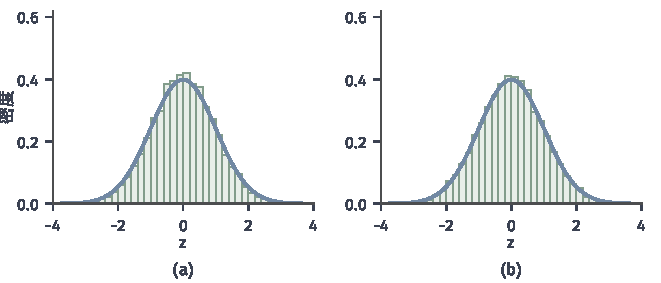
\includegraphics[width=112mm]{figures/07-probability/03-probability-limits/matplotlib/clt-pareto-third/figure.pdf}
 \caption{对称Pareto单项（密度$\frac32\lvert x\rvert^{-4}$，$\lvert x\rvert\geq1$，方差$3$，三阶绝对矩无穷）的标准化和$S_n/\sqrt{3n}$的直方图（浅绿，$20000$次重复，种子$11$）与$\varphi$（蓝）。(a)$n=10$；(b)$n=1000$。}
 \label{fig:clt-pareto-third}
\end{BookInlineFigure}

这个例子与第~\ref{sec:clt-lyapunov}节的比较是同一回事：收敛只看二阶矩，速度要看更高阶的矩。说“$n$足够大时可以用正态近似”之前，应当先问单项分布有没有有限的三阶矩，比值$\rho/\sigma^3$有多大，以及要计算的是典型区间的概率还是罕见事件的概率。


\section{本章小结}
\label{sec:clt-summary}

本章从掷硬币的正面次数出发，问许多独立小项之和的波动服从什么规律。第一步是选对中心和尺度：部分和的典型偏差按$\sigma\sqrt{n}$增长，平均的典型偏差按$\sigma/\sqrt{n}$缩小，只有放大$\sqrt{n}$倍的平均偏差才有不退化也不发散的极限。大数律确定了中心，中心极限定理刻画的是放大以后的形状；标准化只把均值和方差固定为$0$和$1$，形状接近钟形是独立求和的结果，特制硬币的Poisson极限说明了这一点。

在独立同分布、方差有限且为正的条件下，标准化部分和依分布趋于$\mathcal{N}(0,1)$。证明把和的特征函数写成$n$个相同因子的乘积：独立性给出乘积，中心化消去一次项，方差为一固定二次项，二阶矩有限经支配收敛使累计余项可以忽略，连续性定理把特征函数的收敛变回分布的收敛。各项分布不同时，以行内总方差$s_n^2$归一化，Lindeberg条件要求大值贡献的方差份额趋于零；Lyapunov条件用$2+\delta$阶矩换来更方便的核验。这些都是充分条件，各项为高斯而最大项占一半方差的例子说明它们不是必要的。

随机向量的情形由方向投影化为标量：正方差方向用标量定理，零方差方向的投影几乎必然为零，再由Cramér--Wold判据合成协方差为$\bm{\Sigma}$的联合高斯极限，$\bm{\Sigma}$可以奇异。骰子频率的极限就是一个集中在超平面上的退化高斯分布。

\begin{BookInlineTable}
 \centering
 \caption{本章的高斯极限与误差界}
 \label{tab:clt-summary}
 \begin{tabular}{lll}
 \toprule
 结论 & 对象 & 条件 \\
 \midrule
 定理~\ref{thm:clt-iid} & $Z_n$ & 独立同分布，$0<\sigma^2<\infty$ \\
 定理~\ref{thm:clt-lindeberg} & $S_n/s_n$ & 行内独立，Lindeberg条件 \\
 定理~\ref{thm:clt-lyapunov} & $S_n/s_n$ & 行内独立，$\Lambda_n(\delta)\to0$ \\
 定理~\ref{thm:clt-multivariate} & $\sqrt{n}(\bar{\bm{X}}_n-\bm{\mu})$ & 独立同分布，二阶矩有限 \\
 定理~\ref{thm:clt-berry-esseen} & $D_n\leq C\rho/(\sigma^3\sqrt{n})$ & 独立同分布，$\rho<\infty$ \\
 \bottomrule
 \end{tabular}
\end{BookInlineTable}

极限的存在不等于有限样本的精度。Berry--Esseen界在三阶绝对矩有限时给出对所有阈值一致的绝对误差$C\rho/(\sigma^3\sqrt{n})$，速度$1/\sqrt{n}$在格点分布上不能改进；对光滑的分布它可能偏保守。它不控制小尾概率的相对误差，偏斜分布在三四个标准差以外的尾概率可以与高斯近似相差数十倍；三阶矩无穷时，定理仍然成立，误差界却无从调用。

使用这些结论时，先确认中心与尺度，再看独立结构是同分布、三角阵还是向量，然后按要回答的问题核对矩条件：只问极限，二阶矩或Lindeberg条件就够了；要给定样本量下的误差，需要三阶矩；要罕见事件的概率，应回到精确分布或指数矩上界。第~\ref{chap:monte-carlo-integration-error}章将用本章的结论描述独立Monte Carlo积分的误差。


